%% ------------------------------------------------------------------
%% AUTO-GENERATED by FlattenGlossary.py
%% Source: /Users/junga1/AaltoDictionaryofML.github.io/ADictML_Glossary_English.tex
%% Repo root: /Users/junga1/AaltoDictionaryofML.github.io
%% ------------------------------------------------------------------

% !TeX spellcheck = en_US

\newglossaryentry{imagesegmentation}
{name={image segmentation}, 
	description={Image segmentation\index{image segmentation} refers to the task of 
    		clustering the pixels of an image into a few segments \cite{JungLocalGraphClustering}, \cite{Wren1997}. 
		Each segment is a subset (or cluster) of pixels that are similar to each other in 
		terms of color, texture, or other visual properties. 
		\\ 
 		See also: clustering.}, 
 	first={image segmentation}, 
 	text={image segmentation}
}

\newglossaryentry{stratification}
{name={stratification},
	description={The process of splitting a dataset into subsets, so called strata,
 		according to some key attribute is called stratification\index{stratification} 
		\cite{Everitt2010}, \cite{OxfordStatisticsDictionary}, \cite{oecd2008glossary}. 
 		The goal is to ensure that an machine learning (ML) method performs well for each stratum 
		defined by these attributes. For example, in a medical dataset,
  		we may want to stratify a patient dataset by age groups to ensure that an
  		machine learning (ML) model performs well across all age groups. \\
  		When splitting a dataset into a training set and a validation set, 
  		stratification ensures that both sets have similar distributions of the key attribute. 
  		Without stratification, using a small validation set may underrepresent or 
  		even completely miss data points with a rare attribute, leading to misleading 
  		performance estimates. See Fig. \ref{fig_stratification_dict} for a visual illustration.
 		\begin{figure}[H]
 			\centering
			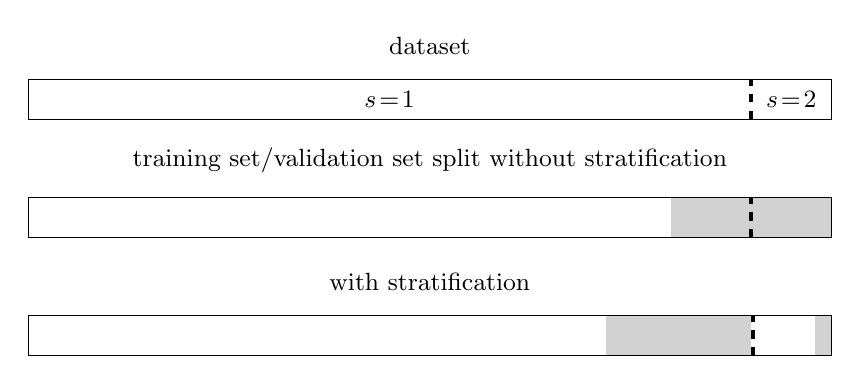
\begin{tikzpicture}[font=\small,x=1.7cm]
			% --- Parameters ---
			\def\cellw{6.0}     % total dataset width
			\def\cellh{0.5}     % height of one row
			\def\gap{1}       % vertical gap between rows
			\def\tfrac{0.8}     % train fraction
			\def\pA{0.9}        % proportion of stratum A (B = 1 - pA)
			% Column labels
			\node[anchor=south] at (0.5*\cellw, \cellh+0.2) {dataset};
			\node[anchor=south] at ({0.5*\cellw}, {-(\cellh+\gap)+\cellh+0.2}) {training set/validation set split without stratification};
			\node[anchor=south] at (0.5*\cellw, {-2*(\cellh+\gap)+\cellh+0.2}) {with stratification};
			% y-positions
			\pgfmathsetmacro{\yDataset}{0}
			\pgfmathsetmacro{\yNoStrat}{-(\cellh+\gap)}
			\pgfmathsetmacro{\yStrat}{-2*(\cellh+\gap)}
			% A/B border x (dataset coordinate)
			\pgfmathsetmacro{\xAB}{\pA*\cellw}
			\pgfmathsetmacro{\wA}{\pA*\cellw}
			\pgfmathsetmacro{\wB}{(1-\pA)*\cellw}
			% --- Row 1: DATASET (only A/B border) ---
			\draw (0,\yDataset) rectangle ++(\cellw,\cellh);
			\draw[dashed,  line width=0.5mm] (\xAB,\yDataset) -- ++(0,\cellh);
			% Labels for strata in Dataset row
			\node at (0.5*\wA, \yDataset+0.5*\cellh) {$s\!=\!1$};
			\node at ({\xAB+0.5*\wB}, {\yDataset+0.5*\cellh}) {$s\!=\!2$};
			%	% --- Row 2: NO STRATIFICATION (shade right 20% as validation) ---
			\draw (0,\yNoStrat) rectangle ++(\cellw,\cellh);
			\pgfmathsetmacro{\xValStart}{\tfrac*\cellw}
			\pgfmathsetmacro{\valw}{(1-\tfrac)*\cellw}
			\fill[gray!35] (\xValStart,\yNoStrat) rectangle ++(\valw,\cellh);
			%	\fill[gray!35] (\xValStart,\yNoStrat) rectangle ++({(1-\tfrac)*\cellw,\cellh});
			%	% A/B border in dataset order only
			\draw[dashed,  line width=0.5mm] (\xAB,\yNoStrat) -- ++(0,\cellh);
			% --- Row 3: STRATIFIED (shade val inside each stratum A and B) ---
			\draw (0,\yStrat) rectangle ++(\cellw,\cellh);
			% A/B border at x = pA * cellw
			\pgfmathsetmacro{\xAB}{\pA*\cellw}
			\draw[dashed, line width=1mm] (\xAB,\yStrat) -- ++(0,\cellh);
			% widths of strata A and B
			% --- Validation area within A (right (1-tfrac) part of A) ---
			\pgfmathsetmacro{\xAVal}{\tfrac*\wA}              % start inside A (A begins at x=0)
			\pgfmathsetmacro{\wAVal}{(1-\tfrac)*\wA}          % width of A's validation
			\fill[gray!35] (\xAVal,\yStrat) rectangle ++(\wAVal,\cellh);
			% --- Validation area within B (right (1-tfrac) part of B) ---
			\pgfmathsetmacro{\xBVal}{\xAB + \tfrac*\wB}       % start inside B
			\pgfmathsetmacro{\wBVal}{(1-\tfrac)*\wB}          % width of B's validation
			\fill[gray!35] (\xBVal,\yStrat) rectangle ++(\wBVal,\cellh);
			\end{tikzpicture}
 		\caption{Stratification ensures that both the training set and the validation set 
			(shaded grey) have similar distributions of a binary key attribute $s$. 
			In other words, with stratification, both strata  
			(i.e., $s\!=\!1$ and $s\!=\!2$ based on the key attribute) 
			allocate the same validation proportion—20\% of their own width. \label{fig_stratification_dict}}
 		\end{figure}
  		See also: stratum, validation, $k$-fold cross-validation ($k$-fold CV).},
  	text={stratification},
  	first={stratification},
  	plural={stratifications}
}

\newglossaryentry{stratum}
{name={stratum},
	description={A\index{stratum} stratum is a subset of data points that all 
		share a common property (which could be a feature or a label). 
		For example, in a weather dataset, all measurements from the same 
		Finnish Meteorological Institute (FMI) weather station form one stratum.
		\begin{center}
			Example (CSV snippet):\\
  			{\ttfamily
  			time, station, value, unit\\
  			2023-06-01 12:00, Helsinki, 18.2, degree Celsius\\
  			2023-06-01 13:00, Helsinki, 18.5, degree Celsius\\
  			2023-06-01 14:00, Helsinki, 19.0, degree Celsius\\
  			2023-06-01 12:00, Oulu, 12.1, degree Celsius\\
  			2023-06-01 13:00, Oulu, 12.4, degree Celsius\\
  			2023-06-01 14:00, Oulu, 12.7, degree Celsius\\
  			2023-06-01 12:00, Tampere, 15.3, degree Celsius\\
  			2023-06-01 13:00, Tampere, 15.6, degree Celsius\\
  			2023-06-01 14:00, Tampere, 16.0, degree Celsius
  			}
		\end{center} 
		Here, the rows for each station (i.e., \texttt{Helsinki}, \texttt{Oulu}, \texttt{Tampere}) 
		represent different strata.
		\\ 
		See also: data point, dataset, stratification.},
  	first={stratum},
  	firstplural={strata},
 	plural={strata}, 
 	text={stratum}
}

\newglossaryentry{attention}
{name={attention}, 
	description={Some machine learning (ML) applications\index{attention} involve data points 
		composed of smaller units, referred to as tokens. For example, a sentence 
		consists of words, an image of pixel patches, and a network of nodes. In general, 
		the tokens that constitute a single data point are not independent 
		of one another. Instead, each token of a data point depends on (or pays attention to) 
		specific other tokens. Probabilistic models provide a principled framework for 
		representing and analyzing such dependencies \cite{Blei2003}. Attention mechanisms use 
		a more direct approach without explicit reference to a probabilistic model. The idea is to 
		represent the relationship between two tokens $i$ and $i'$ 
		using a parameterized function $f^{({\bf w})}(i,i')$, 
		where the parameters ${\bf w}$ are learned via a variant of empirical risk minimization (ERM). 
		Practical attention mechanisms differ in their precise choice of attention model $f^{({\bf w})}(i,i')$ 
		as well as in the precise empirical risk minimization (ERM) variant used to learn the parameters ${\bf w}$. 
		One widely used family of attention mechanisms 
		defines the parameters ${\bf w}$ in terms of two vectors associated with each token $i$, i.e.,
		a query vector ${\bf q}^{(i)}$ and a key vector ${\bf k}^{(i')}$. For a given token $i$ 
		with query ${\bf q}^{(i)}$ and another token $i'$ with key ${\bf k}^{(i')}$, the quantity 
		$\big( {\bf q}^{(i)} \big)^{\top} {\bf k}^{(i')}$ indicates the extent to which token $i$ attends 
		to (or depends on) token $i'$ (see Fig. \ref{fig_attention_dict}).
		\begin{figure}[H]
			\centering
			\begin{tikzpicture}[>=stealth, node distance=0.2cm and 0.2cm,
			every node/.style={inner sep=2pt, font=\large}, baseline]
			% Words (sentence: All human beings are born free and equal.)
			\node (w1) [draw, fill=gray!10, rounded corners] {All};
			\node (w2) [draw, fill=gray!10, right=of w1, rounded corners] {human};
			\node (w3) [draw, fill=gray!10, right=of w2, rounded corners] {beings};
			\node (w4) [draw, fill=gray!10, right=of w3, rounded corners] {are};
			\node (w5) [draw, fill=gray!10, right=of w4, rounded corners] {born};
			\node (w6) [draw, fill=gray!10, right=of w5, rounded corners] {free};
			\node (w7) [draw, fill=gray!10, right=of w6, rounded corners] {and};
			\node (w8) [draw, fill=blue!20, right=of w7, rounded corners] {equal};
			% Label "i" below the word "equal"
   	   		\node[font=\footnotesize, below=0.15cm of w8, align=center] (labeli) {$i$ \\ ${\bf q}^{(i)},\ {\bf k}^{(i)}$};
			\node[font=\footnotesize, below=0.15cm of w1, align=center] (labelii) {$i'$ \\ ${\bf q}^{(i')},\ {\bf k}^{(i')}$};
			% Dummy node above for routing attention arrows
	  		\node (eqTop) [above=1.8cm of w8] {};
	 		% Arrows from "equal" to earlier words (drawn above)
	 		\draw[->, thick, opacity=0.3] (w8.north) .. controls +(up:1.0cm) and +(up:1.0cm) .. (w6.north); % to "free"
	 		\draw[->, thick, opacity=0.3] (w8.north) .. controls +(up:1.2cm) and +(up:1.0cm) .. (w5.north); % to "born"
			\draw[->, thick, opacity=1]  (w8.north)  .. controls +(up:1.8cm) and +(up:1.0cm) ..  node[midway, text=black, above] {$f^{({\bf w})}(i,i')$}  (w1.north); % to "All"
			\end{tikzpicture}
			\caption{Attention mechanisms learn a parameterized function $f^{({\bf w})}(i,i')$ to measure 
				how much token $i$ attends to token $i'$. 
				One widely used construction of $f^{({\bf w})}(i,i')$ 
				uses query and key vectors, denoted by ${\bf q}^{(i)}$ and ${\bf k}^{(i)}$, assigned to each 
				token $i$ \cite{vaswani2017attention}. \label{fig_attention_dict}}
		\end{figure}
		See also: token, function, natural language processing (NLP).},
	first={attention},
	text={attention}
}

\newglossaryentry{transformer}
{name={transformer},
	description={In the context of machine learning (ML), the term transformer\index{transformer} 
 		refers to an artificial neural network (ANN) that uses some form of attention mechanism 
 		to capture dependencies among tokens \cite{vaswani2017attention}. 
 		The attention mechanism is what sets transformers apart from 
		previous models used for sequential data such as recurrent neural networks (RNNs). 
		A transformer artificial neural network (ANN) often combines several attention layers 
		via more traditional layer architectures. 
		\\ 
		See also: attention, natural language processing (NLP). }, 
 	first={transformer}, 
 	text={transformer},
 	firstplural={transformers}, 
 	plural={transformers}
}

\newglossaryentry{rnn}
{name={recurrent neural network (RNN)},
	description={An\index{recurrent neural network (RNN)} RNN 
  		is a specific type of artificial neural network (ANN) that is designed for processing 
    		data that consist of a sequence of tokens. 
		An RNN maintains an internal hidden state that is updated recurrently 
		as new tokens are processed. This recurrent dependence allows 
		information to propagate across time steps, making RNNs suitable for 
		tasks such as speech recognition, language modeling, or time series prediction. 
    		However, their inherently sequential computation limits parallelization and 
		is challenging for gradient-based methods. Variants like the long short-term memory (LSTM) 
		and gated recurrent unit (GRU) mitigate these problems.
		\\
		See also: artificial neural network (ANN), token. }, 
 	first={recurrent neural network (RNN)},
 	text={RNN},
 	firstplural={recurrent neural networks (RNNs)}, 
 	plural={RNNs}
}

\newglossaryentry{llm}
{name={large language model (LLM)},
	description={An\index{large language model (LLM)} LLM is an umbrella term for machine learning (ML) 
		methods that use high-dimensional machine learning (ML) models (with billions 
		of model parameters) trained on large collections of text data. 
 		LLMs are used to analyze or generate sequences of tokens that 
               	constitute text data. Many current LLMs use some variant of 
		a transformer that is trained via self-supervised learning, i.e.,
		the training is based on the task of predicting a few words that 
		are intentionally removed from a large text corpus. Thus, we can 
		construct labeled data points simply by selecting some words 
		from a given text as labels and the remaining words as features 
		of data points. This construction requires 
		very little human supervision and allows for generating sufficiently 
		large training sets for LLMs.
		\\ 
		See also: token, transformer, natural language processing (NLP).}, 
  	first={large language model (LLM)}, 
  	firstplural={LLMs}, 
  	text={LLM}, 
  	plural={LLMs} 
}

\newglossaryentry{selfsupervisedlearning}
{name={self-supervised learning},
 	description={Self-supervised learning\index{self-supervised learning} uses some of 
  		the features of a data point as its label. For 
		example, if a data point consists of a sentence within a text document, 
		we can use the last word of the sentence as the label that is 
		to be predicted from all the previous words, which form the features 
		of the data point. A main application of self-supervised learning 
		is in natural language processing (NLP) for the training of LLMs from large collections 
		of text data. 
		\\ 
      		See also: feature, label, large language model (LLM).}, 
   	first={self-supervised learning}, 
   	text={self-supervised learning}
}

\newglossaryentry{attack}
{name={attack},  
	description={An attack\index{attack} on an machine learning system (ML system) refers to an intentional action—either 
		active or passive—that compromises the system's integrity, availability, or confidentiality. 
		Active attacks involve perturbing components such as datasets (via data poisoning) 
		or communication links between devices within an machine learning (ML) application. Passive attacks, 
		such as privacy attacks, aim to infer sensitive attributes without modifying the system. 
		Depending on their goal, we distinguish among denial-of-service attacks, backdoor attacks, and privacy attacks.
		\\
		See also: data poisoning, privacy attack, sensitive attribute, denial-of-service attack, backdoor.},
	plural={attacks}, 
	first={attack},
	firstplural={attacks},
	text={attack}
}

\newglossaryentry{privattack}
{name={privacy attack},
	description={A privacy attack\index{privacy attack} on an machine learning system (ML system) aims to infer 
		sensitive attributes of individuals by exploiting partial access to a trained machine learning (ML) model. 
		One form of a privacy attack is model inversion.
		\\
		See also: attack, sensitive attribute, model inversion, trustworthy artificial intelligence (trustworthy AI), general data protection regulation (GDPR).},
	plural={privacy attacks}, 
	first={privacy attack},
	firstplural={privacy attacks}, 
	text={privacy attack}
}

\newglossaryentry{discrepancy}
{name={discrepancy},
	description={Consider\index{discrepancy} an federated learning (FL) application with networked data 
		represented by an federated learning network (FL network). federated learning (FL) methods use a discrepancy measure 
		to compare hypothesis maps from local models at nodes $i,i'$, 
		connected by an edge in the federated learning network (FL network).
					\\ 
		See also: federated learning (FL), federated learning network (FL network), local model.},
	first={discrepancy},
	firstplural={discrepancies}, 
  	plural={discrepancies}, 
	text={discrepancy}
}

\newglossaryentry{FedRelax}
{name={FedRelax},
	description={FedRelax refers to a generalized total variation minimization (GTVMin)-based federated learning (FL) method\index{FedRelax} for training local models 
		at the devices of an federated learning network (FL network) \cite{JungFLBook}. It is a 
		distributed algorithm that implements a nonlinear variant of the Jacobi method to solve generalized total variation minimization (GTVMin). 
		\\ 
		See also: federated learning (FL), distributed algorithm.},
	first={FedRelax},
	text={FedRelax}
}

\newglossaryentry{fedavg}
{name={federated averaging (FedAvg)},
	description={FedAvg\index{federated averaging (FedAvg)} refers to a family of iterative federated learning (FL) algorithms. 
		It uses a server-client setting and alternates between clientwise local models 
		retraining, followed by the aggregation of updated model parameters at the server 
		\cite{pmlr-v54-mcmahan17a}, \cite{JungFLBook}. The local update at client $i=1, \,\ldots, \,n$ 
		at time $t$ starts from the current model parameters ${\bf w}^{(t)}$ provided 
		by the server and typically amounts to executing few iterations of stochastic gradient descent (SGD). 
		After completing the local updates, they are aggregated 
		by the server (e.g., by averaging them). Fig. \ref{fig_single_iteration_fedavg_dict} illustrates 
		the execution of a single iteration of FedAvg. 
		\begin{figure}[H]
			\begin{center}
			\begin{tikzpicture}[>=Stealth, node distance=1cm and 1.5cm, every node/.style={font=\small}]
			% Styles
			\tikzstyle{server} = [circle, fill=black, minimum size=6pt, inner sep=0pt]
			\tikzstyle{client} = [circle, draw=black, minimum size=6pt, inner sep=0pt]
			% Time step labels
			\node (label1) at (0,3.5) {broadcast};
			\node[right=2.5cm of label1] (label2) {local update};
			\node[right=2.5cm of label2] (label3) {aggregate};
			% Time step k
			\node[server] (s1) at (label1 |- 0,2.5) {};
			\node[client] (c1l) at ($(s1) + (-1cm,-1cm)$) {};
			\node[client] (c1r) at ($(s1) + (1cm,-1cm)$) {};
			\node[] (dots1) at ($(s1) + (0cm,-1cm)$) {\ldots};
			\draw[->] (s1) -- (c1l) node[midway,left] {${\bf w}^{(t)}$};
			\draw[->] (s1) -- (c1r) node[midway,right] {${\bf w}^{(t)}$};
			\draw[->] (s1) -- (dots1);
			% Time step k+1 (local updates)
			\node[server] (s2) at (label2 |- 0,2.5) {};
			\node[client] (c2l) at ($(s2) + (-1cm,-1cm)$) {};
			\node[client] (c2r) at ($(s2) + (1cm,-1cm)$) {};
			\node[] (dots2) at ($(s2) + (0cm,-1cm)$) {\ldots};
			\node[below=0.2cm of c2l] {$\mathbf{w}^{(t,1)}$};
			\node[below=0.2cm of c2r] {$\mathbf{w}^{(t,n)}$};
			% Time step k+2 (aggregation)
			\node[server] (s3) at (label3 |- 0,2.5) {};
			\node[above=0.01cm of s3, yshift=-4pt] {${\bf w}^{(t+1)}$};
			\node[client] (c3l) at ($(s3) + (-1cm,-1cm)$) {};
			\node[client] (c3r) at ($(s3) + (1cm,-1cm)$) {};
			\node[] (dots3) at ($(s3) + (0cm,-1cm)$) {\ldots};
			\draw[->] (c3l) -- (s3) node[midway,left] {$\mathbf{w}^{(t,1)}$};
			\draw[->] (c3r) -- (s3)  node[midway,right] {$\mathbf{w}^{(t,n)}$};
			\draw[->] (dots3) -- (s3);
			\end{tikzpicture}
			\end{center}
		\caption{Illustration of a single iteration of FedAvg, which consists of broadcasting model parameters by the 
			server, performing local updates at clients, and aggregating the updates by the server. 
			\label{fig_single_iteration_fedavg_dict}} 
		\end{figure} 
		See also: federated learning (FL), algorithm, local model, stochastic gradient descent (SGD).},
	first={federated averaging (FedAvg)},
	text={FedAvg}
} 

\newglossaryentry{FedGD}
{name={federated gradient descent (FedGD)},
	description={FedGD refers to  an\index{federated gradient descent (FedGD)} federated learning (FL) distributed algorithm that 
		can be implemented as message passing across an federated learning network (FL network) \cite{JungFLBook}. 
		\\ 
		See also: federated learning (FL), distributed algorithm, federated learning network (FL network), gradient step, gradient-based method.},
	first={federated gradient descent (FedGD)},
	text={FedGD}
} 

\newglossaryentry{FedSGD}
{name={federated stochastic gradient descent (FedSGD)},
	description={FedSGD refers to an\index{federated stochastic gradient descent (FedSGD)} federated learning (FL) distributed algorithm that 
		can be implemented as message passing across an federated learning network (FL network) \cite{JungFLBook}. 
		\\ 
		See also: federated learning (FL), distributed algorithm, federated learning network (FL network), gradient step, gradient-based method, stochastic gradient descent (SGD).},
	first={federated stochastic gradient descent (FedSGD)},
	text={FedSGD}
} 

\newglossaryentry{hfl}
{name={horizontal federated learning (HFL)},
	description={HFL\index{horizontal federated learning (HFL)} uses local datasets constitut\-ed by different
	   	data points but uses the same features to characterize them \cite{HFLChapter2020}.
		For example, weather forecasting uses a network of spatially distributed
		weather (observation) stations. Each weather station measures the
		same quantities, such as daily temperature, air pressure, and precipitation.
		However, different weather stations measure the characteristics or
		features of different spatiotemporal regions. Each spatiotemporal region 
		represents an individual data point, each characterized by the same features 
		(e.g., daily temperature or air pressure).
		\\
		See also: semi-supervised learning (SSL), federated learning (FL), vertical federated learning (VFL).},
	first={horizontal federated learning (HFL)},
	text={HFL}
} 

\newglossaryentry{dimred}
{name={dimensionality reduction},
	description={Dimensionality reduction\index{dimensionality reduction} refers 
		to methods that learn a transformation 
		$h: \mathbb{R}^{d} \rightarrow \mathbb{R}^{d'}$ 
		of a (typically large) set of raw features $\feature_{1}, \,\ldots, \,\feature_{d}$ 
		into a smaller set of informative features $z_{1}, \,\ldots, \,z_{d'}$. 
		Using a smaller set of features is beneficial in several ways: 
		\begin{itemize} 
			\item {Statistical benefit:} It typically reduces the risk of overfitting, as 
			reducing the number of features often reduces the effective dimension of a model. 
			\item {Computational benefit:} Using fewer features means less computation 
			for the training of machine learning (ML) models. As a case in point, linear regression methods 
			need to invert a matrix whose size is determined by the number of features. 
			\item {Visualization:} Dimensionality reduction is also instrumental for data visualization. 
			For example, we can learn a transformation that delivers two features $z_{1},z_{2}$, 
			which we can use, in turn, as the coordinates of a scatterplot. Fig.\ \ref{fig:dimred-scatter_dict} 
			depicts the scatterplot of handwritten digits that are placed 
			using transformed features. Here, the data points are 
			naturally represented by a large number of greyscale values (one value for each pixel).
		\end{itemize} 
		 \begin{figure}[H]
		 \centering
		 \begin{tikzpicture}[scale=1]	
		% % Axes
		 	\draw[->] (-0.5,0) -- (5.5,0) node[right] {$z_1$};
		 	\draw[->] (0,-0.5) -- (0,4.5) node[above] {$z_2$};
		% % Example points with mini-images (can replace adjustbox with \includegraphics)
		 	\foreach \x/\y/\label in {
  		 		1.2/0.5/3,
  		 		0.8/2.0/8,
  		 		2.5/1.8/1,
  		 		3.8/3.5/6,
  		 		4.2/0.7/9,
  		 		2.8/3.0/7,
  		 		1.5/3.8/2
		 	}{
  		 		\node[draw, minimum size=0.6cm, inner sep=0pt] at (\x,\y)
    	 		{\label};
		 	}
		 	\end{tikzpicture}
		 	\caption{Example of dimensionality reduction: High-dimensional image data 
			(e.g., high-resolution images of handwritten digits) embedded into 2-D using 
			learned features $(z_1, z_2)$ and visualized in a scatterplot.}
		 	\label{fig:dimred-scatter_dict}
		 \end{figure}
		See also: overfitting, autoencoder, random projection, principal component analysis (PCA), Johnson--Lindenstrauss lemma (JL lemma).}, 
	first={dimensionality reduction},
	text={dimensionality reduction}
} 

\newglossaryentry{diagnosis}
{name={diagnosis},
	description={Consider\index{diagnosis} an empirical risk minimization (ERM)-based method that resulted in a trained model 
		(or learned hypothesis) $\hat{h}\in \mathcal{H}$. We can diagnose the 
		method by comparing the training error $E_{t}$ with the validation error $E_{v}$ 
		incurred by $\hat{h}$ on the training set and the validation set. 
		\begin{figure}[H]
			\begin{center}
			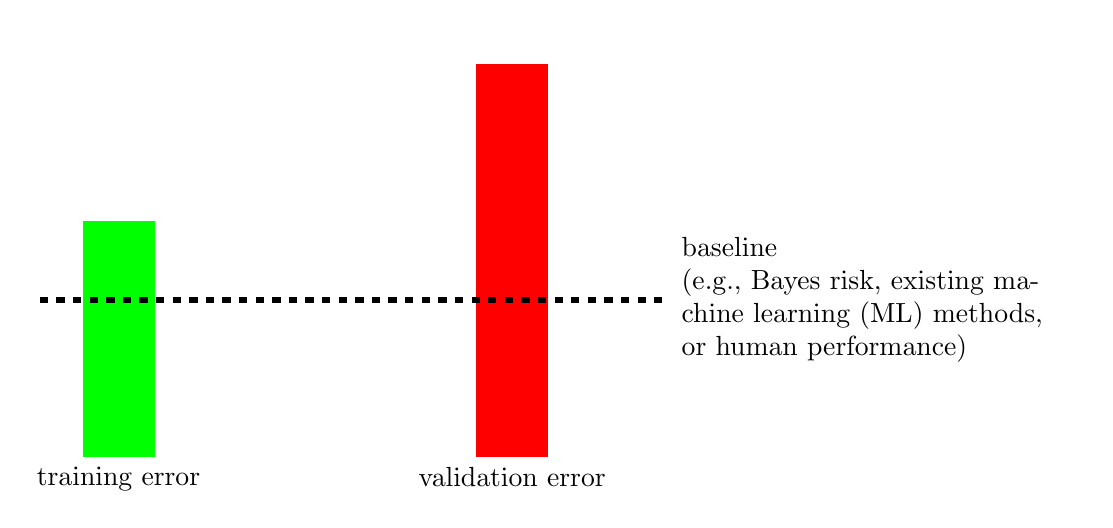
\begin{tikzpicture}[ycomb]
				\draw[color=green,line width=26pt]
				plot coordinates{(0,3)};
				\node [below] at (0,0) {training error} ; 
				\draw[color=red,line width=26pt]
				plot coordinates{(5,5)};
				\node [below] at (5,0) {validation error} ; 
				\draw[dashed,line width=2] (-1,2) -- (7,2) node[right,text width=5cm]{baseline \\ (e.g., Bayes risk, existing machine learning (ML) methods, or human performance)};
			\end{tikzpicture}
			\end{center}
		\caption{We can diagnose an empirical risk minimization (ERM)-based machine learning (ML) method by comparing its training error 
			with its validation error. Ideally, both are on the same level as a baseline.\label{fig_diagnosis_dict}}
		\end{figure}
		See also: baseline, validation, $k$-fold cross-validation ($k$-fold CV), generalization.},
	first={diagnosis},
	text={diagnosis}
} 

\newglossaryentry{ml}
{name={machine learning (ML)},
	description={ML\index{machine learning (ML)} methods aim to learn (or find) 
		a useful hypothesis map $\hat{h}\!\in\!\mathcal{H}$ out of 
		a model $\mathcal{H}$. The learned $\hat{h}$ is used to compute 
		a prediction $\hat{y}=\hat{h}({\bf x})$ for 
		the label $y$ of a data point. The learning process is guided 
		by a quantitative measure of the loss incurred when  
		the predictions obtained from the learned hypothesis differ from  
		the actual label $y$. Different ML methods use different 
		design choices for this quantitative measure (or loss function) as well as 
		different choices for the model and the data points (i.e., 
		their features and labels) \cite[Ch. 3]{MLBasics}. 
		\begin{figure}[H]
			\centering
			\hspace*{5mm}
			\begin{tikzpicture}[
				node distance=1cm,
				auto,
				punkt/.style={
				rectangle,
				rounded corners,
				draw=black,
				very thick,
				text width=3cm,
				minimum height=1cm,
				align=center
				}
				]
				\coordinate (OR) at (0.00, 1.50);
				% concentric circles
				\node[circle,inner sep=0,minimum size={6cm}](a) at (OR) {};
				\node[circle,inner sep=0,minimum size={8cm}](b) at (OR) {};
				\node[circle,inner sep=0,minimum size={8cm}](c) at (OR) {};
				% arcs and radii
				\draw[red,line width=1,dashed] (a.-150) arc (-150:{-150+120}:3cm);
				\draw[blue,line width=1,dashed] (b.160) arc (160:{160+50}:4cm);
				\draw[black!30!green,line width=2,dashed] (c.20) arc (20:{160}:4cm);
				\draw[black!30!blue,line width=2,dashed] ([shift={(-30:6cm)}]OR) arc (-30:{20}:6cm);
				\draw[black!30!blue,line width=2,dashed] (OR) --([shift={(-30:6cm)}]OR);
				\draw[black!30!blue,line width=2,dashed] (OR) --([shift={(20:6cm)}]OR);
				\draw[black!30!green,line width=2,dashed] (OR) -- (c.20);
				\draw[black!30!green,line width=2,dashed] (OR) -- (c.160);
				\draw[blue,thin,dashed] (OR) -- (b.160);
				\draw[blue,thin,dashed] (OR) -- (b.210);
				\draw[red,thin,dashed] (OR) -- (a.-150);
				\draw[red,thin,dashed] (OR) -- (a.-30);   
				% nodes
				\node[punkt] (data) {observations};
				\node[red,below=0.5cm of data] (data1) {data};
				\node[above=of data] (dummy) {};
				\node[punkt,above=1cm of dummy] (hypothesis) {hypothesis};
				\node[right=1.4cm of dummy] (t) {make a prediction} ; 
				\node[left=1.4cm of dummy] (g) {assess and adapt} ;
				\node[blue,below=0.5cm of g,anchor=east] (g1) {loss} ; 
				\node[black!30!blue,below=1cm of t,anchor=west] (g6) {inference} ; 
				\node[black!30!green,above=1cm of hypothesis,anchor=south] (g3) {model} ; 
				% arrows
				\draw [->,line width=0.5mm] (hypothesis.east) to [out=0,in=90] (t.north);
				\draw [->,line width=0.5mm] (t.south) to [out=270,in=0] (data.east);
				\draw [->,line width=0.5mm] (data.west) to [out=180,in=270] (g.south);
				\draw [->,line width=0.5mm] (g.north) to [out=90,in=180] (hypothesis.west);
			\end{tikzpicture}
			\vspace*{-9mm}
		\caption{ML learns a hypothesis out of a model (or hypothesis space) 
			by trying to minimize the loss incurred by the predictions 
			for the labels of data points. The predictions are 
			computed solely from the features of the data points.}
			\label{fig_AlexMLBP_dict}
		\end{figure}
		Another distinction between ML methods is how they access data points during 
		learning. For example, some methods have access to a complete dataset 
		during training, which allows them to use empirical risk minimization (ERM) \cite{MLBasics}, \cite{HastieWainwrightBook}. 
		In contrast, online learning methods access data 
		sequentially and, in turn, update the learned hypothesis 
		whenever a new data point arrives \cite{PredictionLearningGames}, \cite{HazanOCO}, \cite{Bottou99}.
	 			\\ 
		See also: model, loss, data, empirical risk minimization (ERM), online learning.},
	first={machine learning (ML)},
	text={ML}
}

\newglossaryentry{featlearn}
{name={feature learning},
	description={Consider an machine learning (ML) application with data points characterized by 
		raw features ${\bf x}\in \mathcal{X}$. Feature learning\index{feature learning} 
		refers to the task of learning a map 
		$${\bf \Phi}: \mathcal{X}\rightarrow \mathcal{X}': {\bf x}\mapsto {\bf x}'$$ 
		that reads in the features ${\bf x}\in \mathcal{X}$ of a data point and delivers new 
		features ${\bf x}' \in \mathcal{X}'$ from a new feature space $\mathcal{X}'$. 
		Different feature learning methods are obtained for different design 
		choices of $\mathcal{X},\mathcal{X}'$, for a hypothesis space $\mathcal{H}$ 
		of potential maps ${\bf \Phi}$, and for a quantitative measure of the usefulness of 
		a specific ${\bf \Phi}\in \mathcal{H}$. For example, principal component analysis (PCA) 
		uses $\mathcal{X}:=\mathbb{R}^{d}$, $\mathcal{X}' :=\mathbb{R}^{d'}$ 
		with $d' < d$, and a hypothesis space 
		$$\mathcal{H}:=\big\{ {\bf \Phi}: \mathbb{R}^{d}
		\!\rightarrow\! \mathbb{R}^{d'}\!:\!{\bf x}'\!:=\!\mathbf{F}{\bf x}\mbox{ with some } \mathbf{F}\!\in\! \mathbb{R}^{d' \!\times d} \big\}.$$ 
		Principal component analysis (PCA) measures the usefulness of a specific map ${\bf \Phi}({\bf x})= \mathbf{F}{\bf x}$ 
		by the minimum linear reconstruction error incurred on a dataset such that 
		$$\min_{\mathbf{G}\in \mathbb{R}^{d\!\!\!\times d'}} \sum_{r=1}^{m} \mleft\lVert \mathbf{G}\mathbf{F}{\bf x}^{(r)} - {\bf x}^{(r)} \mright\rVert_{2}^{2}.$$ 
			\\ 
		See also: feature, feature space, hypothesis space, principal component analysis (PCA).}, 
	first={feature learning},
	text={feature learning}
}

\newglossaryentry{encoder} 
{name={encoder}, 
	description={See autoencoder\index{encoder}.}, 
 	first={encoder}, 
 	plural={encoders}, 
 	text={encoder}, 
 	firstplural={encoders}
}

\newglossaryentry{autoencoder}
{name={autoencoder},
	description={An autoencoder\index{autoencoder} is an machine learning (ML) method that simultaneously 
		learns an encoder map $h\in \mathcal{H}$ and a decoder map 
		$h^{*} \in \mathcal{H}^{*}$. Different autoencoders use different 
		models $\mathcal{H}, \mathcal{H}^{*}$, e.g., ANNs with different architectures. 
        		The special case of an autoencoder using (vector-valued) linear models for 
		$\mathcal{H}, \mathcal{H}^{*}$ results in principal component analysis (PCA). 
		\begin{figure}[H]
			\centering
			\begin{tikzpicture}[>=Latex, thick, node distance=1.6cm]
			% Nodes
			\node (x) {${\bf x}$};
			\node[draw, rounded corners, right=of x, inner sep=4pt] (enc) {$\text{encoder } h$};
			\node[right=of enc] (z) {${\bf z}$};
			\node[draw, rounded corners, right=of z, inner sep=4pt] (dec) {$\text{decoder } h^{*}$};
			\node[right=of dec] (xhat) {$\hat{{\bf x}}$};
			% Arrows
			\draw[->] (x) -- (enc);
			\draw[->] (enc) -- node[above] {${\bf z}=h({\bf x})$} (z);
			\draw[->] (z) -- (dec);
			\draw[->] (dec) -- node[above] {$\hat{{\bf x}}=h^{*}({\bf z})$} (xhat);
			% (Optional) reconstruction loss
			%\draw[->, dashed] ($(xhat.south)+(0,-0.2)$) to[bend right=20] node[below] {$\loss$} ($(x.south)+(0,-0.2)$);
			\end{tikzpicture}
		\caption{Autoencoder with an encoder $h$ mapping ${\bf x}\mapsto {\bf z}$ and 
			a decoder $h^*$ mapping ${\bf z}\mapsto \hat{{\bf x}}$.}
		\end{figure}
		The training of the encoder and decoder can be implemented via empirical risk minimization (ERM) using a loss that measures 
		the deviation of the reconstructed feature vector $h^{*}\big(h\big({\bf x}\big) \big)$
		from the original feature vector ${\bf x}$.
					\\ 
		See also: encoder, feature learning, dimensionality reduction.},
	first={autoencoder},
	text={autoencoder}
} 

\newglossaryentry{modelparallelism}
{name={model parallelism},
	description={Model parallelism\index{model parallelism} refers to a particular 
        		class of distributed optimization methods used to train an machine learning (ML) model.  
		Here, different devices store and process disjoint subsets of the 
             	model parameters. This approach contrasts with data parallelism, where each 
             	device maintains a full replica of the model parameters while 
             	processing disjoint subsets of the global dataset. 
             	Model parallelism allows us to train an machine learning (ML) model whose 
		parameters cannot fit into the memory of a single device. 
             	One key application of model parallelism is the training of 
            	extremely large ANNs, such as transformer models with 
             	billions of model parameters. 
             	\\
             	See also: vertical federated learning (VFL).},
 	first={model parallelism},
 	text={model parallelism}
}

\newglossaryentry{dataparallelism}
{name={data parallelism},
	description={Data parallelism\index{data parallelism} refers to a widely used 
 		class of distributed optimization methods for training an machine learning (ML) 
             	model. Here, each participating device stores a full 
             	replica of the model parameters but processes a disjoint subset of 
             	the global dataset \cite{DistrOptStatistLearningADMM}. 
             	Compared to model parallelism, which distributes the 
             	model parameters across devices, data parallelism distributes 
             	the computational workload associated with large datasets. 
             	It is especially effective when the model fits into the memory 
             	of a single device, but the dataset or training complexity 
		would be prohibitive without parallel processing. 
             	\\
             	See also: model parallelism, horizontal federated learning (HFL).},
 	first={data parallelism},
 	text={data parallelism}
}

\newglossaryentry{perplexity}
{name={perplexity},
	description={The\index{perplexity} perplexity of an random variable (RV) $x$ is defined as $e^{H_{x}}$.
         	\\
             	See also: entropy.},
 	first={perplexity},
 	text={perplexity}
}

\newglossaryentry{vfl}
{name={vertical federated learning (VFL)},
	description={In VFL,\index{vertical federated learning (VFL)} different devices have 
		access to different features of the same set of data points \cite{VFLChapter}. 
		Formally, the underlying global dataset is
		\[
		\mathcal{D}^{(\mathrm{global})} :=\left\{ \left({\bf x}^{(1)}, y^{(1)}\right), \,\ldots, \,\left({\bf x}^{(m)}, y^{(m)}\right) \right\}.
		\]
		We denote by ${\bf x}^{(r)} = \big( x^{(r)}_{1}, \,\ldots, \,x^{(r)}_{d'} \big)\,^{T}$, for $r=1, \,\ldots, \,m$, 
	     	the complete feature vectors for the data points. Each device $i\in \mathcal{V}$ 
		observes only a subset $\mathcal{F}^{(i)} \subseteq \{1, \,\ldots, \,d'\}$ of features, resulting 
		in a local dataset $\mathcal{D}^{(i)}$ with feature vectors
		\[
		{\bf x}^{(i,r)} = \big( x^{(r)}_{\featureidx_{1}}, \,\ldots, \,x^{(r)}_{\featureidx_{d}} \big)\,^{T}.
		\]
		Some of the devices may also have access to the labels $y^{(r)}$, for $r=1, \,\ldots, \,m$, 
		of the global dataset (see Fig. \ref{fig_vertical_FL_dict}). 
		\begin{figure}[H]
			\begin{center}
			\begin{tikzpicture}[every node/.style={anchor=base}]
				  % --- Coordinate definitions ---
				\def\colX{0}
				\def\colY{1.6}
				\def\colZ{3.2}
				\def\colD{4.8}
				\def\colLabel{6.4} 
				\def\rowOne{0}
				\def\rowTwo{-1.2}
				\def\rowThree{-2.4}
				\def\rowFour{-3.6}
				% Manually place matrix entries
				\foreach \i/\label in {1/1, 2/2, 4/m} {
					\pgfmathsetmacro{\y}{-1.2*(\i-1)}
					\node (x\i1) at (0,\y) {$x^{(\label)}_{1}$};
					\node (x\i2) at (1.6,\y) {$x^{(\label)}_{2}$};
					\node (dots\i) at (3.2,\y) {$\cdots$};
					\node (x\i3) at (4.8,\y) {$x^{(\label)}_{d}$};
					\node (y\i) at (6.4,\y) {$y^{(\label)}$};
				}
				% Outer rectangle for the full dataset
				\draw[dashed, rounded corners, thick]
				(-0.6,0.6) rectangle (6.9,-4.2);
				\node at (3.1,0.9) {$\mathcal{D}^{(\mathrm{global})} $};
				% Rectangle for local dataset 1 (e.g., first two features)
				\draw[dashed, rounded corners, thick]
				(-0.9,0.9) rectangle (2.1,-4.0);
				\node at (0.25,1.0) {$\mathcal{D}^{(1)}$};
		  		% --- Local dataset k (columns 2–3, rows 1–3) ---
				\draw[dashed, rounded corners, thick]
				($( \colZ + 1,,0.9 )$) rectangle
				($( \colLabel + 0.4, -4.5)$);
				\node at ($( \colZ + 0.9,-5 )$) {$\mathcal{D}^{(i)}$};
			\end{tikzpicture}
			\end{center}
		\caption{VFL uses local datasets that are derived from the data points of a common global dataset. 
			The local datasets differ in the choice of features used to characterize 
			the data points.\label{fig_vertical_FL_dict}}
		\end{figure}
		One potential application of VFL is to enable collaboration between 
		different healthcare providers. Each provider collects distinct types of measurements—such as blood 
		values, electrocardiography, and lung X-rays—for the same patients. Another 
		application is a national social insurance system, where health records, financial 
		indicators, consumer behavior, and mobility data are collected by different 
		institutions. VFL enables joint learning across these parties while allowing 
		well-defined levels of privacy protection. We can view VFL as a specific form of
		model parallelism.
		\\
		See also: privacy protection, federated learning (FL), model parallelism.},
	first={vertical federated learning (VFL)},
	text={VFL}
} 

\newglossaryentry{interpretability}
{name={interpretability},
	description={An machine learning (ML) method is interpretable\index{interpretability} for a 
 		human user if they can comprehend the decision process of the method. 
		One approach to develop a precise definition of interpretability is via the concept  
 		of simulatability, i.e., the ability of a human to mentally simulate the model behavior 
		\cite{Colin:2022aa}, \cite{Chen2018}, \cite{doshi2017towards}, \cite{hase-bansal-2020-evaluating}, \cite{Lipton2018}. 
 		The idea is as follows: If a human user understands an machine learning (ML) method, then they should 
 		be able to anticipate its predictions on a test set. We illustrate 
 		such a test set in Fig. \ref{fig_aug_simulatability_dict}, which also depicts 
		two learned hypotheses $\hat{h}$ and $\hat{h}'$. 
		The machine learning (ML) method producing the hypothesis $\hat{h}$ is interpretable
		to a human user familiar with the concept of a linear map. 
    		Since $\hat{h}$ corresponds to a linear map, the user can 
		anticipate the predictions of $\hat{h}$ on the 
		test set. In contrast, the machine learning (ML) method delivering $\hat{h}'$ 
		is not interpretable, because its behavior is no longer aligned with the user’s 
		expectations.
 		\begin{figure}[H]
 			\begin{center} 
			\begin{tikzpicture}[x=1.5cm, y=1cm]
  			% Adjustable parameters
 			\def\slope{0.4}
  			\def\offset{2.0}
  			% Axes
  			\draw[->, very thick] (0,0.5) -- (7.7,0.5) node[below, xshift=-1cm] {$x$}; % x-axis
 			\draw[->, very thick] (0.5,0) -- (0.5,4.2) node[above] {$y$};           % y-axis
  			% Model line
  			\draw[color=black, thick, dashed, domain=-0.5:7.2, variable=\x] 
    			plot ({\x},{\slope*\x + \offset});
			% non-interpretable model
  			\draw[color=black, thick, dashed, domain=4:7.2, variable=\x] 
    			plot ({\x},{\slope*\x + \offset-(\x-4)*0.5});
  			\node[above] at (7.2, {\slope*7.2 + \offset}) {$\hat{h}(x)$};
  			\node[above] at (7.2, {\slope*7.2 + \offset - 0.5*(7.2 - 4)}) {$\hat{h}'(x)$};
 			%\node[above] at (7.2, {\slope*7.2 + \offset-(7.2-4)*0.3}) {$\learnthypothesis'(\feature)$};
  			% Training Data points
  			\foreach \x/\y/\c/\s in {
      			1.2/1.0/blue/6, 1.4/1.0/blue/6, 1.7/1.0/blue/6,
      			2.2/3.9/blue/12, 2.6/4.2/blue/12, 3.0/4.4/blue/12
  			}{
    			\coordinate (pt) at (\x,\y);
    			\node[fill=\c, circle, draw, minimum size=\s pt, scale=0.6] at (pt) {};
    			\draw[<->, >={Latex[width=2mm,length=4mm]}, color=\c, thick]
      			(\x, {\slope*\x + \offset}) -- (pt);
  			}
  			% test set with pseudo-labels
    			\foreach \x/\y/\c/\s in {
       			5.7/2.6/red/12, 5.9/2.6/red/12, 6.2/2.6/red/12
   			}{
     			\coordinate (pt) at (\x,{\slope*\x + \offset});
     			\node[fill=\c, circle, draw, minimum size=\s pt, scale=0.6] at (pt) {};
   			}
  			% Legend
  			\draw[fill=blue] (4.2, 1.7) circle (0.1cm) node [black,xshift=0.2cm,anchor=west] {training set $\mathcal{D}$};
  			\draw[fill=red]  (4.2, 1.2) circle (0.1cm) node [black,xshift=0.2cm,anchor=west] {test set $\mathcal{D}'$};
			\end{tikzpicture}
 			\caption{We can assess the interpretability of trained machine learning (ML) models 
 			$\hat{h}$ and $\hat{h}'$ by comparing their predictions 
			to pseudo-labels generated by a human user for $\mathcal{D}'$. 
			\label{fig_aug_simulatability_dict}}
 			\end{center}
	 	\end{figure} 
 	 	The notion of interpretability is closely related to the notion of explainability, 
 	 	as both aim to make machine learning (ML) methods more understandable for humans. 
		In the context of Fig. \ref{fig_aug_simulatability_dict}, interpretability of an machine learning (ML) 
	 	method $\hat{h}$ requires that the human user can anticipate its predictions 
	 	on an arbitrary test set. This contrasts with explainability, where the user is supported by 
	 	external explanations—such as saliency maps or reference examples from the training set—to 
		understand the predictions of $\hat{h}$ on a specific test set $\mathcal{D}'$. 
	 	\\ 
	 	See also: explainability, trustworthy artificial intelligence (trustworthy AI), regularization, LIME. },
	first={interpretability},
 	text={interpretability}
}

\newglossaryentry{multitask learning}
{name={multitask learning},
	description={Multitask learning\index{multitask learning} aims to leverage relations between 
	 	different learning tasks. Consider two learning tasks obtained from the 
	 	same dataset of webcam snapshots. The first task is to predict the presence 
	 	of a human, while the second task is to predict the presence of a car. It may be useful 
	 	to use the same deep net structure for both tasks and only allow the weights of 
	 	the final output layer to be different.
	 			\\ 
		See also: learning task, dataset, deep net, weight, layer.},
	first={multitask learning},
	text={multitask learning}
}

\newglossaryentry{learningtask}
{name={learning task},
	description={Consider\index{learning task} a dataset $\mathcal{D}$ consisting of 
		multiple data points ${\bf z}^{(1)},\,\ldots,\,{\bf z}^{(m)}$. 
		For example, $\mathcal{D}$ can be a collection of images in an image database. 
		A learning task is defined by specifying those properties (or attributes) of a data point 
		that are used as its features and labels. Given a choice of model $\mathcal{H}$ and 
		loss function, a learning task leads to an instance of empirical risk minimization (ERM) and can thus be 
		represented by the associated objective function $\widehat{L}\big(h|\mathcal{D}\big)$ for $h\in \mathcal{H}$. 
		Importantly, multiple distinct learning tasks can be constructed from the same dataset 
		by selecting different sets of features and labels (see Fig. \ref{fig:learning_tasks_cows_dict}).
    		\begin{figure}[H]
			\centering
			% Top row: image
			\begin{minipage}[t]{0.95\textwidth}
    			\centering
    			\includegraphics[width=\textwidth]{assets/CowsAustria.jpg}
    			\caption*{An image showing cows grazing in the Austrian countryside.}
			\vspace{5mm}
			\end{minipage}
			\vspace{5mm}
			% Bottom row: two learning tasks
			\begin{minipage}[t]{0.45\textwidth}
    			Task 1 (regression): \\
        			Features are the RGB values of all image pixels,
        			and the label is the number of cows depicted.
			\end{minipage}
			\hfill
			\begin{minipage}[t]{0.45\textwidth}
    			Task 2 (classification): \\
			Features include the average green intensity of the image, 
        			and the label indicates whether cows should be moved to another location (i.e., yes/no).
			\end{minipage}
			\caption{Two learning tasks constructed from a single image dataset. 
			These tasks differ in feature selection and choice of label (i.e., the objective), 
			but are both derived from the same dataset.}
			\label{fig:learning_tasks_cows_dict}
		\end{figure}
		Different learning tasks arising from the same underlying dataset are often coupled. 
		For example, when a probabilistic model is used to generate data points, statistical 
		dependencies among different labels induce dependencies among the corresponding 
		learning tasks. In general, solving learning tasks jointly, e.g., using multitask learning 
		methods, tends to be more effective than solving them independently (thereby ignoring 
		dependencies among learning tasks) \cite{Caruana:1997wk}, \cite{JungGaphLassoSPL}, \cite{CSGraphSelJournal}.
	 			\\ 
		See also: multitask learning, label space.},
	first={learning task},
	firstplural={learning tasks},
	plural={learning tasks}, 
	text={learning task}
}

\newglossaryentry{explainability}
{name={explainability},
	description={We\index{explainability} define the (subjective) explainability of an machine learning (ML) method 
		as the level of simulatability \cite{Colin:2022aa} of the predictions 
		delivered by an machine learning system (ML system) to a human user. Quantitative measures of the 
		(subjective) explainability of a trained model can be constructed by 
		comparing its predictions with the predictions provided by a user 
		on a test set \cite{Colin:2022aa}, \cite{Zhang:2024aa}. Alternatively, we can use 
		probabilistic models for data and measure the explainability of a trained machine learning (ML) 
		model via the conditional (or differential) entropy of its predictions, given the 
		user's predictions \cite{JunXML2020}, \cite{Chen2018}.
						\\ 
		See also: trustworthy artificial intelligence (trustworthy AI), regularization.},
	first={explainability},
	text={explainability}
}

\newglossaryentry{lime}
{name={local interpretable model-agnostic explanations (LIME)},
	description={Consider\index{local interpretable model-agnostic explanations (LIME)} 
		a trained model (or learned hypothesis) $\widehat{h} \in \mathcal{H}$, 
		which maps the feature vector of a data point to the prediction $\widehat{y}= \widehat{h}$. 
		LIME is a technique for explaining the behavior of $\widehat{h}$ 
		locally around a data point with feature vector ${\bf x}^{(0)}$ \cite{Ribeiro2016}. 
		The explanation is given in the form of a local approximation $g \in \mathcal{H}'$ of $\widehat{h}$ 
		(see Fig. \ref{fig_lime_dict}). This approximation can be obtained by an instance of empirical risk minimization (ERM) 
		with a carefully designed training set. In particular, the training set consists of data points with 
		feature vectors centered around ${\bf x}^{(0)}$ and the (pseudo-)label $\widehat{h}({\bf x})$. 
		Note that we can use a different model $\mathcal{H}'$ for the approximation from 
		the original model $\mathcal{H}$. For example, we can use a decision tree 
		to locally approximate a deep net. Another widely used choice for $\mathcal{H}'$ is 
		the linear model. 
		\begin{figure}[H]
		\begin{center}
		\begin{tikzpicture}
			\begin{axis}[
				axis lines=middle,
				xlabel={${\bf x}$},
				ylabel={$y$},
				xtick=\empty,
				ytick=\empty,
				xmin=0, xmax=6,
				ymin=0, ymax=6,
				domain=0:6,
				samples=100,
				width=10cm,
				height=6cm,
				clip=false
			]
			% Nonlinear model h(x)
  			\addplot[blue, thick, domain=0:6] {2 + sin(deg(x))} node[pos=0.85, above right,yshift=3pt] {$\widehat{h}({\bf x})$};
			% Feature value x0
  			\addplot[dashed, gray] coordinates {(3,0) (3,6)};
			% Piecewise constant local approximation g(x)
  			\addplot[red, thick, domain=2.5:3.5] {2 + sin(deg(3))} node[pos=0.9, above] {$g({\bf x})$};
			% Optional: mark the point of approximation
  			\addplot[mark=*] coordinates {(3, {2 + sin(deg(3))})};
			\node at (axis cs:3,-0.3) {${\bf x}^{(0)}$};
			\end{axis}
		\end{tikzpicture}
		\end{center}
		\caption{To explain a trained model $\widehat{h} \in \mathcal{H}$, around a 
			given feature vector ${\bf x}^{(0)}$, we can use a local approximation $g \in \mathcal{H}'$. }
			\label{fig_lime_dict}
		\end{figure}
		See also: model, explanation, empirical risk minimization (ERM), training set, label, decision tree, deep net, linear model.},
	first={LIME},
	text={LIME}
}

\newglossaryentry{linmodel}
{name={linear model}, 
	description={Consider\index{linear model} an machine learning (ML) application involving data points, each represented 
		by a numeric feature vector ${\bf x}\in \mathbb{R}^{d}$. A linear model defines 
		a hypothesis space consisting of all real-valued linear maps from $\mathbb{R}^{d}$ to $\mathbb{R}$ such that
		\begin{equation}
			\nonumber
			\label{equ_def_lin_model_hypspace_dict}
			\mathcal{H}^{(d)} :=\left\{ h: \mathbb{R}^{d} \rightarrow \mathbb{R} \mid h({\bf x}) = {\bf w}^{\top} {\bf x}\text{ for some } {\bf w}\in \mathbb{R}^{d} \right\}.
		\end{equation}
		Each value of $d$ defines a different hypothesis space, corresponding to the number of 
		features used to compute the prediction $h({\bf x})$. The choice of 
		$d$ is often guided not only by computational aspects (e.g., fewer features reduce computation) and 
		statistical aspects (e.g., more features typically reduce bias and risk), but also by interpretability. 
		A linear model using a small number of well-chosen features is generally considered 
		more interpretable \cite{rudin2019stop}, \cite{Ribeiro2016}.
		The linear model is attractive because it can typically be trained using scalable convex 
		optimization methods \cite{BertsekasNonLinProgr}, \cite{hastie01statisticallearning}. 
		Moreover, linear models often permit rigorous 
		statistical analysis, including fundamental limits on the minimum achievable risk \cite{Wain2019}. 
		They are also useful for analyzing more complex nonlinear models such as ANNs. For instance, 
		a deep net can be viewed as the composition of a feature map—implemented by the input and 
		hidden layers—and a linear model in the output layer. Similarly, a decision tree can be interpreted 
		as applying a one-hot-encoded feature map based on decision regions, followed by a linear 
		model that assigns a prediction to each region.
		More generally, any trained model $\hat{h}\in \mathcal{H}$ that is 
		differentiable at some ${\bf x}'$ can be locally approximated by a linear map 
		$g({\bf x})$. Fig.~\ref{fig_linapprox_dict} illustrates such a local linear approximation, 
		defined by the gradient $\nabla \hat{h}({\bf x}')$. Note that the gradient 
		is only defined where $\hat{h}$ is differentiable.
		To ensure robustness in the context of trustworthy artificial intelligence (trustworthy AI), one may prefer models whose 
		associated map $\hat{h}$ is Lipschitz continuous. A classic result in mathematical 
		analysis—Rademacher’s theorem—states that if $\hat{h}$ is Lipschitz continuous with 
		some constant $L$ over an open set $\Omega\subseteq \mathbb{R}^{d}$, then $\hat{h}$ 
		is differentiable almost everywhere in $\Omega$ \cite[Th.~3.1]{heinonen2005lectures}.
		\begin{figure}[H]
			\begin{center}
			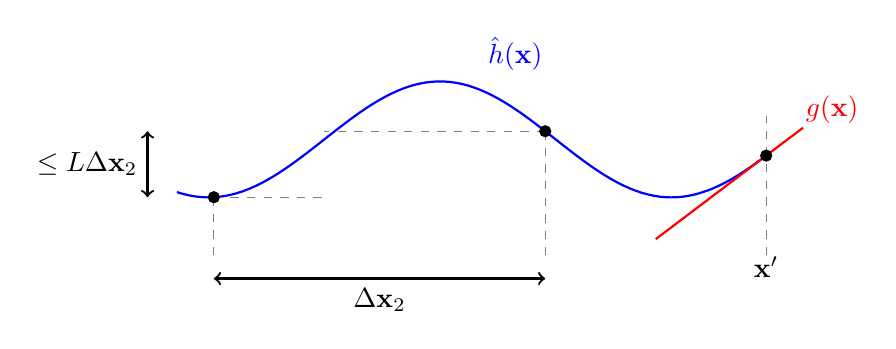
\begin{tikzpicture}[x=0.5cm]
			\begin{axis}[
			hide axis,
			xmin=-3, xmax=6,
			ymin=0, ymax=6,
			domain=0:6,
			samples=100,
			width=10cm,
			height=6cm,
			clip=false
			]
			% Original nonlinear function h(x)
			\addplot[blue, thick, domain=-2:6] {2 + sin(deg(x))} 
			node[pos=0.5, above right, yshift=3pt] {$\hat{h}({\bf x})$};
			% Tangent line as local linear approximation at x = 3
			% h(3) = 2 + sin(3), h'(3) = cos(3)
			\addplot[red, thick, domain=4.5:6.5] 
			{2 + sin(deg(6)) + cos(deg(6))*(x - 6)}
			node[pos=0.95, above right] {$g({\bf x})$};
			% Mark point of approximation
			\addplot[mark=*] coordinates {(6, {2 + sin(deg(6))})};
			% Vertical dashed line (ruler) at x = 3
			\addplot[dashed, gray] coordinates {(6,0) (6,2.4)};
			\node at (axis cs:6, -0.2) {${\bf x}'$};
			% Plot the two points
			% Coordinates of the two points
			\pgfmathsetmacro{\xA}{-1.5}
			\pgfmathsetmacro{\xB}{3}
			\pgfmathsetmacro{\yA}{2 + sin(deg(\xA))}
			\pgfmathsetmacro{\yB}{2 + sin(deg(\xB))}
			\addplot[mark=*, only marks] coordinates {(\xA, \yA) (\xB, \yB)};
			%	\node at (axis cs:\xA, \yA+0.2) {$A$};
			%	\node at (axis cs:\xB, \yB+0.2) {$B$};
			% Draw dashed lines from the points to the x and y axes
			\draw[dashed, gray] (axis cs:\xA,\yA) -- (axis cs:\xA,0);
			\draw[dashed, gray] (axis cs:\xB,\yB) -- (axis cs:\xB,0);
			\draw[dashed, gray] (axis cs:\xA,\yA) -- (axis cs:0,\yA);
			\draw[dashed, gray] (axis cs:\xB,\yB) -- (axis cs:0,\yB);
			 % Draw delta x
			\draw[<->, thick] (axis cs:\xA,-0.4) -- node[below] {$\mleft\lVert \Delta {\bf x}\mright\rVert_{2}$} (axis cs:\xB,-0.4);
			% Draw delta y
			\draw[<->, thick] (axis cs:-2.4,\yA) -- node[left] {$\leq L \mleft\lVert \Delta {\bf x}\mright\rVert_{2}$} (axis cs:-2.4,\yB);
			\end{axis}
			\vspace*{-10mm}
			\end{tikzpicture}
			\vspace*{-5mm}
			\end{center}
		\caption{A trained model $\hat{h}({\bf x})$ that is differentiable at a point ${\bf x}'$ 
			can be locally approximated by a linear map $g \in \mathcal{H}^{(d)}$. This local approximation 
			is determined by the gradient $\nabla \hat{h}({\bf x}')$.}
			\label{fig_linapprox_dict}
		\end{figure}
		See also: model, hypothesis space, linear map, interpretability, LIME.}, 
   first={linear model},
   plural={linear models},
   firstplural={linear models}, 
   text={linear model}
}

\newglossaryentry{earlystopping}
{name={early stopping}, 
	description={Consider an empirical risk minimization (ERM)-based method that uses an 
		iterative optimization method (such as gradient descent (GD)) to learn model parameters 
		by minimizing the empirical risk on a given training set.
		Early stopping\index{early stopping} refers to terminating the iterations 
		even if they still substantially decrease the empirical risk on the 
		training set. Instead of monitoring the objective function (which is the 
		empirical risk on the training set), early stopping monitors the validation error 
		incurred by the model parameters in each iteration. Early stopping can be 
		interpreted as an implementation of regularization via model 
		pruning. Indeed, terminating an iterative optimization method after a small number 
		of iterations restricts the set of model parameters that can be reached from the 
		initialization (see Fig.\ \ref{fig_early_stopping_dict}).
		\begin{figure}[H]
		\centering
			\begin{tikzpicture}[>=Stealth, scale=2]
			% Initialization
			\fill (0,0) circle (0.6pt) node[above] {\small ${\bf w}^{(0)}$};
			\node at (-0.4,0) {\small $\mathcal{H}^{(1)}$};
			\node at (-1.2,0) {\small $\mathcal{H}^{(2)}$};
			\node at (-2,0) {\small $\mathcal{H}\ldots$};
			% T-step reachable sets (early stopping = smaller T)
			\draw[densely dotted] (0,0) ellipse (0.8 and 0.4);
			\draw[dashed] (0,0) ellipse (1.6 and 0.8);
			% Example gradient path (just illustrative)
			\draw[->] (0,0) -- (0.8,0.) node [pos=0.6,above] {\tiny $1$ step};
			\draw[->] (0.0,0.0) -- (0,-0.8) node [pos=0.9,right] {\tiny $2$ steps};
			\end{tikzpicture}
		\caption{A gradient-based method for empirical risk minimization (ERM) using a hypothesis space $\mathcal{H}$ 
		    	defines a nested sequence of effective hypothesis spaces 
			$\mathcal{H}^{(1)} \subseteq \mathcal{H}^{(2)} \subseteq \ldots \subseteq \mathcal{H}$. 
			The effective hypothesis space $\mathcal{H}^{(t)}$ is 
		    	determined by all model parameters that can be reached from the initialization 
			${\bf w}^{(0)}$ within $t$ gradient steps. \label{fig_early_stopping_dict}}
		\end{figure}
		See also: regularization, gradient-based method, overfitting.},
	first={early stopping},
	text={early stopping}
}

\newglossaryentry{statasp}
{name={statistical aspect}, 
	description={By statistical aspects\index{statistical aspect} 
		of an machine learning (ML) method, we refer to (properties of) the probability distribution of its output 
		under a probabilistic model for the data fed into the method.
					\\ 
		See also: machine learning (ML), probability distribution, probabilistic model, data.},
	firstplural={statistical aspects},
	plural={statistical aspects},
	first={statistical aspect},
	text={statistical aspect}
}

\newglossaryentry{compasp}
{name={computational aspect}, 
	description={By computational 
		aspects\index{computational aspect} of an machine learning (ML) method, we mainly refer to the computational 
		resources required for its implementation. For example, if an machine learning (ML) method uses iterative 
		optimization techniques to solve empirical risk minimization (ERM), then its computational aspects include: 1) how 
		many arithmetic operations are needed to implement a single iteration (i.e., a gradient step); 
		and 2) how many iterations are needed to obtain useful model parameters. One important 
		example of an iterative optimization technique is gradient descent (GD).
					\\ 
		See also: machine learning (ML), empirical risk minimization (ERM), gradient step, model parameter, gradient descent (GD).}, 
	first={computational aspect},
	text={computational aspect},
	firstplural={computational aspects},
	plural={computational aspects}
}

\newglossaryentry{zerooneloss}
{name={$\bf 0/1$ loss},
sort={zerooneloss}, 
	description={The $0/1$ loss\index{$0/1$ loss} $L^{(0/1)}\left(\left( {\bf x},y\right),h\right)$ 
		measures the quality of a classifier $h({\bf x})$ that delivers a 
		prediction $\hat{y}$ (e.g., via thresholding \eqref{equ_def_threshold_bin_classifier_dict}) 
		for the label $y$ of a data point with features ${\bf x}$. It is equal to $0$ if 
		the prediction is correct, i.e., 
		$L^{(0/1)}\left(\left( {\bf x},y\right),h\right)=0$ when $\hat{y}=y$. It is 
		equal to $1$ if the prediction is wrong, i.e., $L^{(0/1)}\left(\left( {\bf x},y\right),h\right)=1$ 
		when $\hat{y}\neqy$.
				\\ 
		See also: loss, classifier, prediction, accuracy, label, data point, feature.},
    	first={$0/1$ loss},
	text={$0/1$ loss}
}

\newglossaryentry{probability}
{name={probability}, 
	description={We\index{probability} assign a probability value, typically chosen in the 
		interval $[0,1]$, to each event that can occur in a random experiment  
		\cite{BillingsleyProbMeasure}, \cite{BertsekasProb}, \cite{KallenbergBook}, \cite{HalmosMeasure}.
		\\
		See also: event, random experiment. },
	first={probability},
	firstplural={probabilities},
	plural={probabilities},
	text={probability}
}
	
\newglossaryentry{underfitting}
{name={underfitting},
	description={Consider\index{underfitting} an machine learning (ML) method applying empirical risk minimization (ERM) 
		to learn a hypothesis that minimizes the empirical risk 
		on a given training set. The method is said to underfit if it fails to achieve a sufficiently low empirical risk on the training set. 
		Underfitting typically occurs when the chosen model is too simple 
		to capture the underlying relationship between features and labels. 
		\begin{figure}[H]
		\begin{center}
			\begin{tikzpicture}[scale=1.0]
				% Hypothesis: simple linear map (underfits)
				\def\slope{0.35}
				\def\intercept{2.0}
				\draw[thick,dashed,domain=0:6.5,variable=\x]
				plot({\x},{\slope*\x+\intercept});
				\node[above right] at (6.5,{\slope*6.5+\intercept}) {$h(x)$};
				% Nonlinear pattern of data points (suggesting true relation is curved)
				% (x, y) points laid out along a gentle curve
				\foreach \i/\x/\y in {1/0.6/2.4, 2/1.2/2.1, 3/1.8/2.0, 4/2.4/2.3,
					5/3.0/3.1, 6/3.6/4.0, 7/4.2/5.2, 8/4.8/6.0,
					9/5.4/6.3, 10/6.0/6.1} {
					\node[circle,draw,fill=blue!60,minimum size=5pt,inner sep=0pt] (p\i) at (\x,\y) {};
					% residual arrow to dashed hypothesis line
					\draw[<->,color=blue!70] (\x,{\slope*\x+\intercept}) -- (p\i);
				}
			\end{tikzpicture}
		\caption{No linear hypothesis $h$ can capture the relationship 
			between features and labels for 
			the depicted training set. Thus, any method that uses a 
			linear model will underfit this training set.}
			\label{fig_underfitting_min_dict}
		\end{center}
		\end{figure} 
		For example, an machine learning (ML) method using a linear model 
		on data with a highly nonlinear relationship between features 
		and labels will not be able to learn a hypothesis with small 
		average loss on the training set, let alone a low risk. 
					\\ 
		See also: training set, model, risk, overfitting.},
	first={underfitting},
	text={underfitting}
}

\newglossaryentry{overfitting}
{name={overfitting},
	description={Consider\index{overfitting} an 
		machine learning (ML) method that uses empirical risk minimization (ERM) to learn a hypothesis with the 
		minimum empirical risk on a given training set. Such a method is 
		overfitting the training set if it learns a hypothesis with an  
		empirical risk on the training set that is significantly smaller than the 
		average loss outside the training set. In other words, if an machine learning (ML) 
		method overfits, it has a large generalization gap. 
					\\ 
		See also: empirical risk minimization (ERM), generalization, validation, generalization gap.},
	first={overfitting},
	text={overfitting}
}

\newglossaryentry{diffusionmethod}
{name={diffusion method},
	description={A diffusion method is a generative machine learning (ML) method that
		trains a model to approximate the reversal of a gradual stochastic
		corruption process \cite{DeepLearningBishop}, \cite{Prince2023UnderstandingDL}. 
		Diffusion methods train models using a combination of a forward (diffusion) 
		process and a learned reverse map.
		In the forward process, random noise is incrementally added to clean
		representations of a data point, such as an image, an audio recording,
		or other types of data. Similar to a denoising autoencoder, the 
		trained model can be applied to a noisy representation of a data point. 
		The resulting prediction is a denoised representation. What sets 
		diffusion methods apart from generic denoising autoencoders is the gradual 
		nature of the corruption process used for model training.
		\\
		See also: denoising autoencoder, training. },
	first={diffusion method},
    	plural={diffusion methods},
    	firstplural={diffusion methods},
    	text={diffusion method}
}

\newglossaryentry{sqerrloss}
{name={squared error loss},
	description={The squared 
		error\index{squared error loss} loss measures the prediction error of a 
		hypothesis $h$ when predicting a numeric label $y\in \mathbb{R}$ 
		from the features ${\bf x}$ of a data point. It is defined as 
		\begin{equation} 
			\nonumber
			L\left(({\bf x},y),h\right) :=\big(y- \underbrace{h({\bf x})}_{=\hat{y}} \big)^{2}. 
		\end{equation} 
			\\ 
		See also: loss, prediction, hypothesis, label, feature, data point.},
	first={squared error loss},
	text={squared error loss}
}

\newglossaryentry{diffpriv}
{name={differential privacy (DP)},
	description={Consider\index{differential privacy (DP)} some machine learning (ML) method $\mathcal{A}$ 
  		that reads in a dataset (e.g., the training set 
  		used for empirical risk minimization (ERM)) and delivers some output $\mathcal{A}(\mathcal{D})$. The output 
  		could be either the learned model parameters or the predictions for specific data points. 
  		DP is a precise measure of privacy leakage incurred by revealing the 
  		output. Roughly speaking, an machine learning (ML) method is differentially private if the probability distribution 
  		of the output $\mathcal{A}(\mathcal{D})$ remains largely unchanged when the sensitive attribute 
  		of one data point in the training set is changed. Note that DP 
  		builds on a probabilistic model for an machine learning (ML) method, i.e., we interpret its output $\mathcal{A}(\mathcal{D})$ 
  		as the realization of an random variable (RV). The randomness in the output can be ensured 
  		by intentionally adding the realization of an auxiliary random variable (RV) (i.e., adding noise) to 
  		the output of the machine learning (ML) method.
				\\ 
		See also: output, privacy leakage, sensitive attribute, privacy attack, privacy funnel.}, 
  	first={DP}, 
  	text={DP} 
}

\newglossaryentry{robustness}
{name={robustness},
	description={Robustness\index{robustness} is a key requirement for trustworthy artificial intelligence (trustworthy AI). It
		refers to the property of an machine learning system (ML system) to maintain acceptable performance even when 
		subjected to different forms of perturbations. These perturbations may affect the features 
		of a data point in order to manipulate the prediction delivered by a trained machine learning (ML) model. 
		Robustness also includes the stability of empirical risk minimization (ERM)-based methods against perturbations 
		of the training set. Such perturbations can occur within data poisoning attacks. 
		\\ 
		See also: trustworthy artificial intelligence (trustworthy AI), stability, data poisoning, attack.}, 
	first={robustness}, 
	text={robustness} 
}

\newglossaryentry{stability}
{name={stability},
	description={Mathematically, an machine learning (ML) method is a map $\mathcal{A}$ from a given dataset $\mathcal{D}$ 
		to an output $\mathcal{A}(\mathcal{D})$. As a case in point, consider an empirical risk minimization (ERM)-based 
		machine learning (ML) method that maps a training set $\mathcal{D}$ to the learned model parameters 
		$\mathcal{A}(\mathcal{D}) = \widehat{{\bf w}}$, which achieve the minimum average loss 
		on the training set. Instead of the learned model parameters, the 
		output $\mathcal{A}(\mathcal{D})$ could also be the predictions obtained from 
		the trained model. Stability\index{stability} refers to the desirable property 
		of $\mathcal{A}$ that small changes in the input dataset $\mathcal{D}$ result in small 
		changes in the output $\mathcal{A}(\mathcal{D})$. The notion of stability is intimately related 
		to the notion of generalization. In particular, there are formal notions of stability  
		that allow us to bound the generalization gap (see \cite[Ch.~13]{ShalevMLBook}).
		To build intuition, consider the three datasets depicted in Fig. \ref{fig_three_data_stability_dict}, each 
		of which is equally likely under the same data-generating probability distribution. Since the 
		optimal model parameters are determined by this underlying probability distribution, an accurate 
		machine learning (ML) method $\mathcal{A}$ should return the same (or very similar) output $\mathcal{A}(\mathcal{D})$ 
		for all three datasets. In other words, any useful $\mathcal{A}$ must be robust to 
		variability in sample realizations from the same probability distribution, i.e., it must be stable. 
		\begin{figure}[H]
			\centering
			\begin{tikzpicture}
				\begin{axis}[
					%title={Stem Plots of 3 Datasets},
					axis lines=none,
					xlabel={$r$},
					ylabel={},
					legend pos=north west,
					ymin=0, ymax=10,
					xtick={1,2,3,4,5},
					%	ymajorgrids=true,
					grid style=dashed,
					every axis plot/.append style={very thick}
					]
					% Dataset 1
					\addplot+[only marks,mark=*] coordinates {
						(1,2) (2,4) (3,3) (4,5) (5,7)
					};
					%	\addlegendentry{$\dataset^{(*)}$}
					% Dataset 2
					\addplot+[only marks,mark=square*] coordinates {
						(1,3) (2,2) (3,6) (4,4) (5,5)
					};
					%	\addlegendentry{$\dataset^{(\square)}$}
					% Dataset 3
					\addplot+[only marks,mark=triangle*] coordinates {
						(1,5) (2,7) (3,4) (4,6) (5,3)
					};
					%	\addlegendentry{$\dataset^{(\triangle)}$}
				\end{axis}
			\end{tikzpicture}
		\caption{Three datasets $\mathcal{D}^{(*)}$, $\mathcal{D}^{(\square)}$, 
			and $\mathcal{D}^{(\triangle)}$, each sampled independently from the same 
			data-generating probability distribution. A stable machine learning (ML) method should return 
			similar outputs when trained on any of these datasets. \label{fig_three_data_stability_dict}}
		\end{figure}
		See also: generalization, robustness.}, 
	first={stability}, 
	text={stability} 
}

\newglossaryentry{privprot}
{name={privacy protection},
     description={Consider\index{privacy protection} some machine learning (ML) method $\mathcal{A}$ that reads 
	 	in a dataset $\mathcal{D}$ and delivers some output $\mathcal{A}(\mathcal{D})$. The output 
	 	could be the learned model parameters $\widehat{{\bf w}}$ or the prediction 
	 	$\hat{h}({\bf x})$ obtained for a specific data point with features 
	 	${\bf x}$. Many important machine learning (ML) applications involve data points 
		representing humans. Each data point is characterized by features ${\bf x}$, 
		potentially a label $y$, and a sensitive attribute $s$ (e.g., a recent medical diagnosis). 
		Roughly speaking, privacy protection means that it should be impossible to infer, from the output $\mathcal{A}(\mathcal{D})$, 
		any of the sensitive attributes of data points in $\mathcal{D}$. Mathematically, privacy protection requires non-invertibility 
		of the map $\mathcal{A}(\mathcal{D})$. In general, just making $\mathcal{A}(\mathcal{D})$ non-invertible 
		is typically insufficient for privacy protection. We need to make $\mathcal{A}(\mathcal{D})$ sufficiently non-invertible. 
					\\ 
		See also: machine learning (ML), dataset, model parameter, prediction, data point, feature, label, sensitive attribute, map.}, 
	first={privacy protection}, 
	text={privacy protection} 
}

\newglossaryentry{privleakage}
{name={privacy leakage},
	description={Consider\index{privacy leakage} an machine learning (ML) application that processes a 
		dataset $\mathcal{D}$ and delivers some output, such as the predictions 
		obtained for new data points. Privacy leakage arises 
		if the output carries information about a private (or sensitive) feature of 
		a data point of $\mathcal{D}$ (such as a human). Based on a probabilistic model 
		for the data generation, we can measure the privacy leakage via the MI 
		between the output and the sensitive feature. Another quantitative measure of privacy leakage 
		is DP. The relations between different measures of privacy leakage have been 
		studied in the literature (see \cite{InfThDiffPriv}). 
				\\ 
		See also: MI, DP, privacy attack, general data protection regulation (GDPR). }, 
	first={privacy leakage}, 
	text={privacy leakage} 
}

\newglossaryentry{crossentropy}
{name={cross-entropy},
	description={Consider a multi-class classification problem with a 
		feature space $\mathcal{X}$ and a finite label space 
              	$\mathcal{Y}= \{1,\,\ldots,\,k\}$.  A data point with a 
              	feature vector ${\bf x}$ is represented as a probability mass function (pmf) 
              	${\bf y}= (\truelabel_{1},\,\ldots,\,\truelabel_{k})^{T}$ 
              	over~$\mathcal{Y}$, where $\truelabel_{c}$ denotes the 
              	probability that a randomly chosen data point with 
		feature vector ${\bf x}$ has label $c$.  
		A hypothesis $h({\bf x})$ outputs a predicted 
              	probability mass function (pmf) $\hat{{\bf y}} = (\predictedlabel_{1},\,\ldots,
              	\,\predictedlabel_{k})^{T}$. The associated 
              	\index{cross-entropy}cross-entropy loss is \cite{coverthomas} 
             	\begin{equation}
                		\nonumber
                		L\left(({\bf x},\hat{{\bf y}}),h\right)
                		:=- \sum_{c=1}^{k} 
                		\truelabel_{c}\,\log \predictedlabel_{c}.
              	\end{equation}
		The cross-entropy loss quantifies the dissimilarity between the true 
		probability mass function (pmf) ${\bf y}$ and the predicted probability mass function (pmf) $\hat{{\bf y}}$. It is 
		also a measure of the expected number of bits required to encode labels 
		drawn from the true probability mass function (pmf) ${\bf y}$ when using a coding scheme optimized for 
		the predicted probability mass function (pmf) $\hat{{\bf y}}$ \cite{coverthomas}. \\
		Note that, for binary classification (with $k= 2$), the 
              	cross-entropy loss reduces to the logistic loss when 
              	employing a parametric model with model parameters ${\bf w}$ 
              	such that $\predictedlabel_{2}/\predictedlabel_{1}
              	= \exp\,({\bf w}^{T}{\bf x})$. Moreover, the representation 
              	\eqref{equ_log_loss_gls_dict} of logistic loss requires encoding 
              	the label space $\{1,2\}$ using the values $-1$ and $1$. 
			  \\
		See also: classification, probability mass function (pmf), logistic loss. }, 
 	first={cross-entropy},
 	text={cross-entropy}
}

\newglossaryentry{bce}
{name={binary cross-entropy (BCE)},
	description={The\index{binary cross-entropy (BCE)} BCE loss is a 
   		special case of cross-entropy loss for a binary classification problem.
		\\
		See also: cross-entropy, classification. }, 
 	first={binary cross-entropy (BCE)},
 	text={BCE}
}

\newglossaryentry{softlabel}
{name={soft label},
	description={Consider\index{soft label} a classification problem where data points are characterized 
 		by features ${\bf x}$ and labels from a finite label space 
		$\mathcal{Y}= \{1,\,\ldots,\,k\}$. Some machine learning (ML) applications involve data points 
		that have almost identical features but different labels. In such 
		cases, instead of assigning to each data point a single label $y\in \mathcal{Y}$, 
		it can be more useful to assign an entire probability distribution over the label space. 
		This probability distribution can be represented as a probability mass function (pmf) 
		${\bf y}= \big( \truelabel_{1},\,\ldots,\,\truelabel_{k}\big)^{T} \in \Delta^{k}$. 
		We can view the entries $\truelabel_{c}$, for $c=1,\,\ldots,\,k$, 
		as soft labels of a data point. Mathematically, the soft label $\truelabel_{c}$  
		is the probability that a randomly chosen data point with feature vector ${\bf x}$ 
		has label $c$.
		\\
              	See also: classification, probability mass function (pmf), cross-entropy.},
 	first={soft label},
 	plural={soft labels},
 	firstplural={soft labels},
 	text={soft label}
}

\newglossaryentry{nn}
{name={nearest neighbor (NN)},
	description={NN\index{nearest neighbor (NN)} methods learn a hypothesis 
		$h: \mathcal{X}\rightarrow \mathcal{Y}$ whose function value $h({\bf x})$ 
		is solely determined by the NNs within a given dataset. Different 
		methods use different metrics for determining the NNs. If data points 
		are characterized by numeric feature vectors, we can use their Euclidean distances as 
		the metric.
					\\ 
		See also: metric, neighbor.},
	first={nearest neighbor (NN)},
	plural={NNs},
 	firstplural={nearest neighbors (NNs)},
	text={NN} 
}

\newglossaryentry{neighbor}
{name={neighbor},
	description={A\index{neighbor} neighbor of a node $i\in \mathcal{V}$ 
		within an undirected graph is a node $i' \in \mathcal{V}\setminus \{ i\}$ 
		that is connected via an edge to node $i$.
				\\ 
		See also: undirected graph, connected.},
	first={neighbor},
	firstplural={neighbors}, 
	plural={neighbors}, 
	text={neighbor} 
}

\newglossaryentry{bias}
{name={bias},
	description={Consider\index{bias} an empirical risk minimization (ERM)-based machine learning (ML) method that  
		learns a hypothesis $\hat{h}\in \mathcal{H}$ 
		from a given training set. The analysis of the machine learning (ML) method 
		is often based on a probabilistic model (such as the independent and identically distributed assumption (i.i.d.\ assumption)) 
		for the data generation. Here, data points and, in turn, 
		the learned hypothesis $\hat{h}$ are viewed as 
		(realizations of) random variables (RVs). Any property 
		$\theta\big(\hat{h}\big)$ of $\hat{h}$, 
		such as specific model parameters in a parametric model 
		or the prediction error $y- \hat{h}({\bf x})$ 
		for a fixed data point, then also becomes an random variable (RV). 
		The squared bias of a numeric property $\theta\big(\hat{h}\big) \in \mathbb{R}^{r}$ 
		is \cite{BishopBook}, \cite{hastie01statisticallearning}
		$$B^{2} :=\big\| \mathbb{E} \big\{ \theta\big(\hat{h}\big) \big\}\!-\!\theta\big(\bar{h}\big)  \big\|_{2}^{2}.$$
		Here, $\bar{h}$ is a reference hypothesis, which 
		could be defined by $\bar{h}({\bf x})=y$ 
		for a fixed test data point with feature vector ${\bf x}$ 
		and label $y$. 
					\\ 
		See also: probabilistic model, independent and identically distributed (i.i.d.), random variable (RV), estimation error.},
	first={bias},
	text={bias},
	user1={biased}
}

\newglossaryentry{classification}
{name={classification},
	description={Classification\index{classification} is the task of determining a 
 		discrete-valued label $y$ for a given data point, based solely on its 
 		features ${\bf x}$. The label $y$ belongs to a finite set, such as 
 		$y\in \{-1,1\}$ or $y\in \{1, \,\ldots, \,19\}$, and represents the 
 		category to which the corresponding data point belongs.
				\\ 
		See also: label, data point, feature.}, % \gls{binclass},
	first={classification},
	text={classification} 
}

\newglossaryentry{privfunnel}
{name={privacy funnel},
	description={The\index{privacy funnel} privacy funnel is a method for learning 
		a feature map that provides privacy-friendly features for a 
		data point \cite{PrivacyFunnel}.
				\\ 
		See also: feature, data point, general data protection regulation (GDPR), DP.},
 	first={privacy funnel},
	text={privacy funnel} 
}

\newglossaryentry{classifier}
{name={classifier},
	description={A classifier\index{classifier} is a hypothesis (i.e., a map) $h({\bf x})$ 
		used to predict a label taking on values from a finite label space. We might use the 
		function value $h({\bf x})$ itself as a prediction $\hat{y}$ for 
		the label. However, it is customary to use a map $h(\cdot)$ that delivers 
		a numeric quantity. The prediction is then obtained by a simple thresholding step. 
		For example, in a binary classification problem with a label space $\mathcal{Y}\in  \{ -1,1\}$, 
		we might use a real-valued hypothesis map $h({\bf x}) \in \mathbb{R}$ 
		as a classifier. A prediction $\hat{y}$ can then be obtained via thresholding:
		 \begin{equation} 
		 	\label{equ_def_threshold_bin_classifier_dict}
		 	\hat{y}=1 \quad  \mbox{for } h({\bf x})\!\geq\!0 \quad \mbox{and} \quad	\hat{y}=-1  \quad \mbox{otherwise.}
	 	\end{equation}
 		We can characterize a classifier by its decision regions $\mathcal{R}_{a}$ for 
 		every possible label value $a \in \mathcal{Y}$.
					\\ 
		See also: hypothesis, classification, decision region. },
	first={classifier},
	text={classifier} 
}

\newglossaryentry{emprisk}
{name={empirical risk},
	description={The empirical risk\index{empirical risk} $\widehat{L}\big(h|\mathcal{D}\big)$ 
  		of a hypothesis on a dataset $\mathcal{D}$ is the average loss incurred 
  		by $h$ when applied to the data points in $\mathcal{D}$.
				\\ 
		See also: risk, hypothesis, dataset, loss, data point.},
  	first={empirical risk},
  	text={empirical risk} 
}

\newglossaryentry{token}
{name={token},
	description={A token\index{token} is a basic unit of information 
  		obtained by splitting a sequence of symbols, such as a text string, 
  		into smaller parts. In natural language processing (NLP), tokens often correspond to words, subwords, 
  		or characters that form the features of a data point. 
  		Tokenization transforms raw text (e.g., ``The cat sleeps'') into a 
  		sequence of tokens (e.g., [``The'', ``cat'', ``sleeps'']), which can
  		then be mapped to numerical feature vectors.
		\\
		See also: sequence, feature vector. }, 
  	first={token}, 
  	firstplural={tokens}, 
  	plural={tokens}, 
  	text={token}
}

\newglossaryentry{nlp}
{name={natural language processing (NLP)},
	description={NLP\index{natural language processing (NLP)} 
 		studies machine learning (ML) methods for the the analysis and generation of human language. 
  		Typical NLP tasks include text classification, machine translation, 
  		sentiment analysis, and question answering. Modern NLP systems represent 
  		language as sequences of tokens and train models that 
  		capture contextual dependencies, such as attention-based methods.
		\\ 
  		See also: token, attention.}, 
	first={natural language processing (NLP)}, 
	text={NLP}
}

\newglossaryentry{riskstratification}
{name={risk stratification},
	description={Risk stratification\index{risk stratification} assigns 
		data points to risk groups (or strata) by 
		quantizing the prediction $\hat{h}({\bf x})$ 
		obtained from a trained risk prognosis model. Typical choices for these 
		strata include low, intermediate, and high risk 
             	\cite{Collins:2012aa}, \cite{Steyerberg2019}.
		\\
		See also: stratification, prediction, clustering.},
	first={risk stratification},
	text={risk stratification}
}

\newglossaryentry{uncertainty}
{name={uncertainty},
	description={In the context of machine learning (ML), uncertainty\index{uncertainty} refers to the presence of multiple 
		plausible outcomes or explanations based on available data. For example, the 
		prediction $\hat{h}({\bf x})$ produced by a trained machine learning (ML) model $\hat{h}$
	 	often reflects a range of possible values for the true label of a given data point. 
	 	The broader this range, the greater the associated uncertainty. Probability theory 
	 	allows us to represent, quantify, and reason about uncertainty in a 
	 	mathematically rigorous manner.
					\\ 
		See also: probabilistic model, risk, entropy, variance. },
	first={uncertainty},
	text={uncertainty}
}

\newglossaryentry{ucb}
{name={upper confidence bound (UCB)},
	description={Consider\index{upper confidence bound (UCB)} an machine learning (ML) 
		application that requires selecting, at each time step $t$, an action $\arm_{t}$ 
		from a finite set of alternatives $\mathcal{A}$. The utility of selecting action $\arm_{t}$ 
		is quantified by a numeric reward signal $r^{(\arm_{t})}$. 
		A widely used probabilistic model for this type of sequential decision-making problem 
		is the stochastic multiarmed bandit (stochastic MAB) setting \cite{Bubeck2012}. In this model, 
		the reward $r^{(a)}$ is viewed as the realization of an random variable (RV) 
		with unknown mean $\mu^{(a)}$. Ideally, we would always choose the 
		action with the largest expected reward $\mu^{(a)}$, but these 
		means are unknown and must be estimated from observed data. Simply 
		choosing the action with the largest estimate $\widehat{\mu}^{(a)}$ can 
		lead to suboptimal outcomes due to estimation uncertainty. The UCB strategy 
		addresses this by selecting actions not only based on their estimated means but 
		also by incorporating a term that reflects the uncertainty in these estimates—favoring 
		actions with a high-potential reward and high uncertainty. Theoretical guarantees 
		for the performance of UCB strategies, including logarithmic regret bounds, are established in \cite{Bubeck2012}.
					\\ 
		See also: action, reward, stochastic multiarmed bandit (stochastic MAB), uncertainty, regret, optimism in the face of uncertainty.},
	first={upper confidence bound (UCB)},
	text={UCB} 
}

\newglossaryentry{optimism in the face of uncertainty}
{name={optimism in the face of uncertainty},
	description={machine learning (ML)\index{optimism in the face of uncertainty} methods learn model parameters ${\bf w}$ 
		according to some performance criterion $\bar{f}({\bf w})$. However, they usually 
		cannot access $\bar{f}({\bf w})$ directly but rely on an estimate (or approximation) 
		$f({\bf w})$ of $\bar{f}({\bf w})$. As a case in point, empirical risk minimization (ERM)-based methods use 
		the average loss on a given dataset (i.e., the training set) as an estimate 
		for the risk of a hypothesis. Using a probabilistic model, one can construct 
		a confidence interval $\big[ l^{({\bf w})},  u^{({\bf w})} \big]$ for each choice ${\bf w}$ for the model parameters.
		One simple construction is $l^{({\bf w})} :=f({\bf w}) - \sigma/2$, $u^{({\bf w})} :=f({\bf w})+ \sigma/2$, 
	    	with $\sigma$ being a measure of the (expected) deviation of $f({\bf w})$ from $\bar{f}({\bf w})$.
		We can also use other constructions for this interval as long as they ensure that $\bar{f}({\bf w}) \in\big[ l^{({\bf w})},  u^{({\bf w})} \big]$ 
		with a sufficiently high probability. An optimist chooses the model parameters 
		according to the most favorable—yet still plausible—value $\tilde{f}({\bf w}) :=l^{({\bf w})}$ 
		of the performance criterion (see Fig. \ref{fig_optimism_dict}). Two examples of machine learning (ML) methods that use such an optimistic 
		construction of an objective function are structural risk minimization (SRM) \cite[Ch. 11]{ShalevMLBook} and upper confidence bound (UCB) methods 
		for sequential decision making \cite[Sec. 2.2]{Bubeck2012}. 
		\begin{figure}[H]
			\begin{center}
			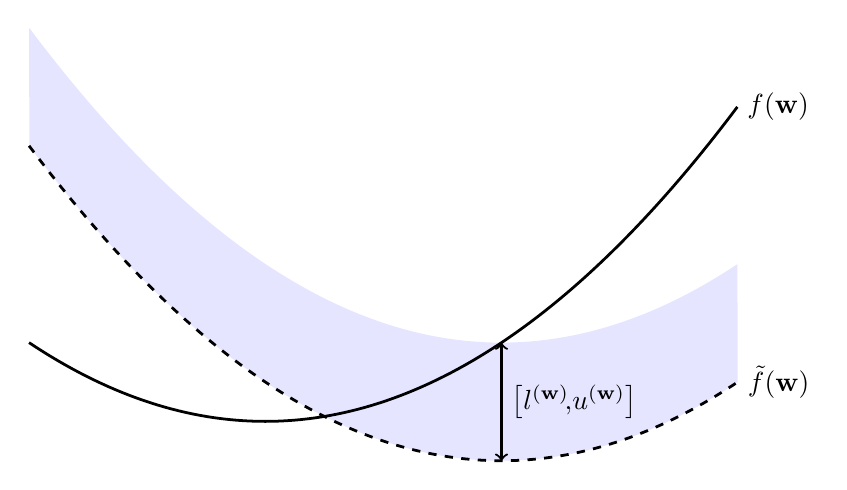
\begin{tikzpicture}[x=3cm, y=1cm]
  			% Filled band around the quadratic curve with different boundary curves
			\fill[blue!10] 
			(-1, 5) -- plot[domain=-2:1, samples=100] ({\x+1}, {\x*\x + 1}) -- 
			plot[domain=1:-2, samples=100] ({\x+1}, {\x*\x - 0.5}) -- cycle;
  			\node[anchor=west] at (2, 4) {$f({\bf w})$};
  			\draw[line width=1, domain=-2:1, samples=100,dashed] plot  ({\x+1}, {\x*\x -0.5}) node[right] {$\tilde{f}({\bf w})$};
   			\draw[line width=1, domain=-1:2, samples=100] plot ({\x}, {\x*\x});
  			\draw[<->, thick] (1, -0.5) -- (1, 1) node[midway, right] {$\big[ l^{({\bf w})}\!,\!u^{({\bf w})} \big]$};
			\end{tikzpicture}
		\caption{machine learning (ML) methods learn model parameters ${\bf w}$ by using some estimate of $f({\bf w})$ for 
			the ultimate performance criterion $\bar{f}({\bf w})$. Using a probabilistic model, one can use $f({\bf w})$ to 
			construct confidence intervals $\big[ l^{({\bf w})},  u^{({\bf w})} \big]$, which contain $\bar{f}({\bf w})$  
			with high probability. The best plausible performance measure for a specific choice ${\bf w}$ of model parameters 
			is $\tilde{f}({\bf w}) :=l^{({\bf w})}$. \label{fig_optimism_dict}} 
			\end{center}
		\end{figure}
		See also: objective function, upper confidence bound (UCB), optimization method, gradient-based method.},
	first={optimism in the face of uncertainty},
	text={optimism in the face of uncertainty} 
}

\newglossaryentry{flnetwork}
{name={federated learning network (FL network)},
	description={An federated learning (FL) network\index{federated learning network (FL network)} is a 
		mathematical model for a federated learning system (FL system) that consists of interconnected 
		devices. These devices are represented by the nodes $\mathcal{V}$ 
		of an undirected weighted graph
		\[
			\mathcal{G}= (\mathcal{V},\mathcal{E},{\bf A}).
		\]
		An edge $\{i,i'\} \in \mathcal{E}$ indicates collaborations 
		between two devices $i, i' \in \mathcal{V}$. 
		The edge weights $\edgeweight_{i,i'} > 0$ 
		quantify the extent of collaborations, which may be related to a 
		communication link capacity, statistical similarity between 
		local datasets, or both. Each device $i\in \mathcal{V}$ 
		has potentially access to a local dataset $\mathcal{D}^{(i)}$ and 
		might train a local model $\mathcal{H}^{(i)}$, e.g., using 
		empirical risk minimization (ERM)-based methods. Many popular federated learning (FL) methods are obtained by 
		coupling the training of these local models across the edges of the 
		federated learning (FL) network \cite{JungFLBook}. This coupling can be implemented in different ways, 
		e.g., using a penalty term that enforces similarity between the model parameters 
		of neighboring devices, or using the predictions of neighboring 
		devices to augment the local datasets.
		Fig.\ \ref{fig_fl_network_dict} illustrates an federated learning (FL) network with four devices.
		\begin{figure}[H]
		\centering
		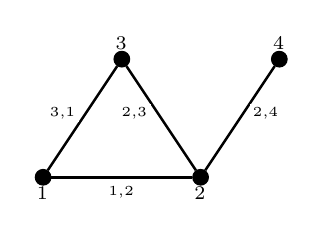
\begin{tikzpicture}[
			scale=1,
			node/.style={circle, draw=black, fill=black, inner sep=2pt},
			edge/.style={line width=0.9pt},
			wlab/.style={fill=white, inner sep=1pt, font=\scriptsize}
			]
			% Nodes
			\node[node] (v1) at (0,0) {};
			\node[node] (v2) at (2,0) {};
			\node[node] (v3) at (1,1.5) {};
			\node[node] (v4) at (3,1.5) {};
			% Labels
			\node[anchor=north] at (v1) {$\nodeidx_1$};
			\node[anchor=north] at (v2) {$\nodeidx_2$};
			\node[anchor=south] at (v3) {$\nodeidx_3$};
			\node[anchor=south] at (v4) {$\nodeidx_4$};
			% Undirected weighted edges + weight labels next to edges
			\draw[edge] (v1) -- node[wlab, pos=0.5, below, yshift=-2pt] {$\edgeweight_{1,2}$} (v2);
			\draw[edge] (v2) -- node[wlab, pos=0.55, left,  xshift=-2pt] {$\edgeweight_{2,3}$} (v3);
			\draw[edge] (v3) -- node[wlab, pos=0.45, left,  xshift=-2pt] {$\edgeweight_{3,1}$} (v1);
			\draw[edge] (v2) -- node[wlab, pos=0.55, right, xshift=2pt] {$\edgeweight_{2,4}$} (v4);
			\end{tikzpicture}
		\caption{An federated learning (FL) network with nodes $\mathcal{V}=\{\nodeidx_1,\nodeidx_2,\nodeidx_3,\nodeidx_4\}$ 
			representing four devices of an federated learning system (FL system). \label{fig_fl_network_dict}}
		\end{figure}
		The federated learning (FL) network specifies which devices can interact and to what extent. 
	    	\\
		See also: federated learning (FL), device, graph, generalized total variation minimization (GTVMin).},
	first={federated learning network (FL network)},
	text={FL network},
	plural={FL networks}, 
	firstplural={federated learning networks (FL networks)}
}

\newglossaryentry{explanation}
{name={explanation},
	description={One approach to enhance the transparency of an machine learning (ML) method for its human user 
		is to provide an explanation\index{explanation} alongside the predictions delivered 
		by the method. Explanations can take different forms. For instance, they may 
        		consist of human-readable text or quantitative indicators, such as feature 
        		importance scores for the individual features of a given data point~\cite{Molnar2019}. 
	   	Alternatively, explanations can be visual—for example, intensity maps that highlight 
	   	image regions that drive the prediction \cite{GradCamPaper}. 
       		Fig.\ \ref{fig_explanation_dict} illustrates two types of explanations. The first 
       		is a local linear approximation $g({\bf x})$ of a nonlinear trained model 
       		$\hat{h}({\bf x})$ around a specific feature vector ${\bf x}'$, 
       		as used in the method LIME. 
        		The second form of explanation depicted in the figure is a sparse set of predictions 
       		$\hat{h}({\bf x}^{(1)}), \hat{h}({\bf x}^{(2)}), \hat{h}({\bf x}^{(3)})$ 
       		at selected feature vectors, offering concrete reference points for the user. 
	 	\begin{figure}[H]
	   		\begin{center}
	 		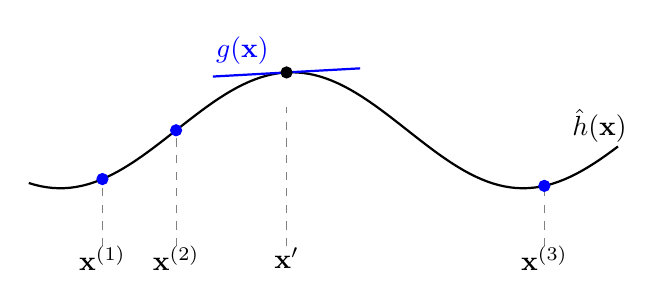
\begin{tikzpicture}[x=0.5cm]
	 		\begin{axis}[
	 			hide axis,
	 			xmin=-3, xmax=6,
	 			ymin=0, ymax=6,
	 			domain=0:6,
	 			samples=100,
	 			width=10cm,
	 			height=6cm,
	 			clip=false
	 		   ]
	 		% Original nonlinear function h(x)
			\addplot[thick, domain=-2:6] {2 + sin(deg(x))} 
	   		node[pos=0.9, above right, yshift=10pt] {$\hat{h}({\bf x})$};
	 		% Tangent line as local linear approximation at x = 1.5
	 		% h(3) = 2 + sin(3), h'(3) = cos(3)
	 		\addplot[blue, thick, domain=0.5:2.5] 
	 		{2 + sin(deg(1.5)) + cos(deg(1.5))*(x - 1.5)}
	 		node[pos=0.2, above] {$g({\bf x})$};
	 		% Mark point of approximation
	 		\addplot[mark=*] coordinates {(1.5, {2 + sin(deg(1.5))})};
	 		    % Vertical dashed line (ruler) at x = 1.5
			\addplot[dashed, gray] coordinates {(1.5,0) (1.5,2.4)};
	 		\node at (axis cs:1.5, -0.2) {${\bf x}'$};
	      		% add function values for finite set of featurevecs
	       		\addplot[mark=*,blue] coordinates {(-1, {2 + sin(deg(-1))})};
	       		\addplot[dashed, gray] coordinates {(-1,0) (-1,{2 + sin(deg(-1))})};
	       		\node at (axis cs:-1, -0.2) {${\bf x}^{(1)}$};
	 	   	\addplot[mark=*,blue] coordinates {(0, {2 + sin(deg(0))})};
	 	   	\addplot[dashed, gray] coordinates {(0,0) (0,{2 + sin(deg(0))})};
	 	   	\node at (axis cs:0, -0.2) {${\bf x}^{(2)}$};
	 	   	\addplot[mark=*,blue] coordinates {(5, {2 + sin(deg(5))})};
	 	   	\addplot[dashed, gray] coordinates {(5,0) (5,{2 + sin(deg(5))})};
	 	   	\node at (axis cs:5, -0.2) {${\bf x}^{(3)}$};
			% 		    % Plot the two points
			% 		    % Coordinates of the two points
			% 		\pgfmathsetmacro{\xA}{-1.5}
			% 		\pgfmathsetmacro{\xB}{3}
			% 		\pgfmathsetmacro{\yA}{2 + sin(deg(\xA))}
			% 		\pgfmathsetmacro{\yB}{2 + sin(deg(\xB))}
	 		\end{axis}
			% 	\vspace*{-10mm}
			\end{tikzpicture}
	 	\end{center}
	 	\caption{A trained model $\hat{h}({\bf x})$ can be explained 
	     		locally at some point ${\bf x}'$ by a linear approximation $g({\bf x})$. 
	     		For a differentiable $\hat{h}({\bf x})$, this approximation is 
	     		determined by the gradient $\nabla \hat{h}({\bf x}')$. Another 
	     		form of explanation could be the function values $\hat{h}\big({\bf x}^{(r)} \big)$ 
	     		for $r=1, \,2, \,3$. 
			\label{fig_explanation_dict}}
	 	\end{figure} 
		See also: machine learning (ML), prediction, feature, data point, classification.},
	first={explanation},
	plural={explanations},
	text={explanation} 
}

\newglossaryentry{risk}
{name={risk},
	description={Consider\index{risk} a hypothesis $h$ used to predict the label 
		$y$ of a data point based on its features ${\bf x}$. We measure 
		the quality of a particular prediction using a loss function $L\left(({\bf x},y),h\right)$. 
		If we interpret data points as the realizations of independent and identically distributed (i.i.d.) random variables (RVs), 
		the $L\left(({\bf x},y),h\right)$ also becomes the realization 
		of an random variable (RV). The independent and identically distributed assumption (i.i.d.\ assumption) allows us to define the risk of a hypothesis 
		as the expected loss $\mathbb{E} \big\{L\left(({\bf x},y),h\right) \big\}$. 
		Note that the risk of $h$ depends on both the specific choice for the loss function and the 
		probability distribution of the data points.
					\\ 
		See also: independent and identically distributed (i.i.d.) random variable (RV), independent and identically distributed assumption (i.i.d.\ assumption), loss, probability distribution.},
	first={risk},
	text={risk} 
}

\newglossaryentry{actfun}
{name={activation function},
	description={Each\index{activation function} artificial neuron within an artificial neural network (ANN) is 
		assigned an activation function $\sigma(\cdot)$ that maps a weighted 
		combination of the neuron inputs $\feature_{1}, \,\ldots, \,\feature_{d}$ 
		to a single output value $a = \sigma\big(\weight_{1} \feature_{1}+\ldots+\weight_{d} \feature_{d} \big)$. 
		Note that each neuron is parameterized by the weights $\weight_{1}, \,\ldots, \,\weight_{d}$.
					\\ 
		See also: artificial neural network (ANN), activation, rectified linear unit (ReLU).},
	first={activation function},
	text={activation function} 
}

\newglossaryentry{distributedalgorithm}
{name={distributed algorithm},
	description={A\index{distributed algorithm} distributed algorithm is an algorithm designed for 
		a special type of computer, i.e., a collection of interconnected computing devices (or nodes). 
		These devices communicate and coordinate their local computations by exchanging 
		messages over a network \cite{IntroDistAlg}, \cite{ParallelDistrBook}. Unlike a classical algorithm, 
		which is implemented on a single device, a distributed algorithm is 
		executed concurrently on multiple devices with computational capabilities. 
		Similar to a classical algorithm, a distributed algorithm can be modeled as a 
		set of potential executions. However, each execution in the distributed setting involves 
		both local computations and message-passing events. A generic execution might look as 
		follows:
		\[
		\begin{array}{l}
			\text{Node 1: } {\rm input}_1, \,s_1^{(1)}, \,s_2^{(1)}, \,\ldots, \,s_{T_1}^{(1)}, \,{\rm output}_1; \\
			\text{Node 2: } {\rm input}_2, \,s_1^{(2)}, \,s_2^{(2)}, \,\ldots, \,s_{T_2}^{(2)}, \,{\rm output}_2; \\
			\quad \vdots \\
			\text{Node N: } {\rm input}_N, \,s_1^{(N)}, \,s_2^{(N)}, \,\ldots, \,s_{T_N}^{(N)}, \,{\rm output}_N.
		\end{array}
		\]
		Each device $i$ starts from its own local input and performs a sequence of 
		intermediate computations $s_{t}^{(i)}$ at discrete-time instants $t= 1, \,\dots, \,T_i$. 
		These computations may depend on both the previous local computations at the device 
		and the messages received from other devices. One important application of distributed 
		algorithms is in federated learning (FL) where a network of devices collaboratively trains a personal model 
		for each device. 
					\\ 
		See also: algorithm, device, event, federated learning (FL), model.},
	first={distributed algorithm}, 
	text={distributed algorithm}
}

\newglossaryentry{algorithm}
{name={algorithm},
 	description={An\index{algorithm} algorithm is a precise, step-by-step specification for 
  		producing an output from a given input within a finite number of well-defined 
		computational steps \cite{Cormen:2022aa}. For example, a gradient-based method for linear regression 
		is an algorithm that explicitly describes how to map a given training set 
		into model parameters through a sequence of gradient steps. The precise form of 
		an algorithm depends on the available computational infrastructure. For example, if 
		this infrastructure allows us to compute an inverse matrix, then we can 
		define a linear regression algorithm using the normal equations. In contrast, if 
		the computational infrastructure only allows basic arithmetic operations (i.e., multiplication and addition), 
		the normal equations need to be somehow translated into a sequence of arithmetic 
		operations (e.g., as in gradient-based methods). 
		To study algorithms rigorously, we can represent (or approximate) them by different 
		mathematical structures \cite{Sipser2013}. One approach is to represent an algorithm 
		as a collection of possible executions. Each individual execution is then a 
		sequence of the following form: $${\rm input}, \,s_1, \,s_2, \,\ldots, \,s_T, \,{\rm output}.$$ 
		This sequence starts from an input and progresses via intermediate steps until an 
		output is delivered. Crucially, an algorithm encompasses more than just a mapping 
		from input to output; it also includes intermediate computational 
     		steps $s_1, \,\ldots, \,s_T$.
				\\ 
		See also: output, linear regression, training set, model parameter, gradient step, model, stochastic.},
	first={algorithm},
	plural={algorithms},
	text={algorithm} 
}

\newglossaryentry{stochalgorithm}
{name={stochastic algorithm},
	description={A\index{stochastic algorithm} stochastic algorithm uses a random mechanism 
		during its execution. For example, stochastic gradient descent (SGD) uses a randomly selected subset of data points 
		to compute an approximation for the gradient of an objective function. We can represent a 
		stochastic algorithm by a stochastic processes, i.e., the possible execution sequence is the possible outcomes of 
		a random experiment \cite{BertsekasProb}, \cite{RandomizedAlgos}, \cite{Gallager13}.		
		\\ 
		See also: stochastic, algorithm, stochastic gradient descent (SGD), data point, gradient, objective function, stochastic process, 
		random experiment, optimization method, gradient-based method. },
	first={stochastic algorithm},
	text={stochastic algorithm},
	plural={stochastic algorithms},
	firstplural={stochastic algorithms}
}

\newglossaryentry{batchlearning}
{name={batch learning},
	description={In batch learning\index{batch learning} (also known as offline learning), the machine learning (ML) model 
		is trained on the entire dataset in a single training iteration, instead of updating it incrementally as data arrive. 
		All available data are inputted into a learning algorithm, resulting in a model that can make predictions. 
		Since these datasets tend to be large, training is computationally expensive and time-consuming, 
		so it is typically performed offline. After learning, the model will be static and will not adapt to new data automatically. 
		Updating the model with new information requires retraining the model entirely. Once the model has been trained, 
		it is launched into production where it cannot be updated. Training a model can take many hours, so many models in production 
		settings are updated cyclically on a periodic schedule when the data distribution is stable. For example, a retail analytics team 
		could retrain their demand forecast model every Sunday using the previous week's sales data to predict next week's demand. 
		If a system needs to be constantly updated to rapidly changing data, such as in stock price prediction, a more adaptable solution 
		such as online learning is necessary.
		\\
		See also: batch, model, dataset, online learning. },
	first={batch learning}, 
	text={batch learning}
}

\newglossaryentry{onlinelearning}
{name={online learning},
	description={Some machine learning (ML) methods\index{online learning} are designed to 
	    	process data in a sequential manner, updating their model parameters 
		one at a time, as new data points become available. A typical example 
		is time-series data, such as daily minimum and maximum 
		temperatures recorded by an Finnish Meteorological Institute (FMI) weather station. These values form 
		a chronological sequence of observations. During each time step $t$, 
		online learning methods update (or refine) the current hypothesis 
		$h^{(t)}$ (or model parameters ${\bf w}^{(t)}$) 
		based on the newly observed data point ${\bf z}^{(t)}$. 
		\\ 
		See also: online gradient descent (online GD), online algorithm. },
	first={online learning},
	text={online learning} 
}

\newglossaryentry{onlinealgorithm}
{name={online algorithm},
	description={An\index{online algorithm} online algorithm processes input data incrementally, 
		receiving data points sequentially and making decisions or producing outputs (or decisions) immediately 
		without having access to the entire input in advance \cite{PredictionLearningGames}, \cite{HazanOCO}. 
		Unlike an offline algorithm, which has the entire input available from the start, an online algorithm 
		must handle uncertainty about future inputs and cannot revise past decisions. Similar to an 
		offline algorithm, we represent an online algorithm formally as a collection of possible 
		executions. However, the execution sequence for an online algorithm has a distinct structure as follows:
		$${\rm in}_{1}, \,s_1, \,{\rm out}_{1}, \,{\rm in}_{2}, \,s_2, \,{\rm out}_{2}, \,\ldots, \,{\rm in}_{T}, \,s_T, \,{\rm out}_{T}.$$ 
		Each execution begins from an initial state (i.e., \(\text{in}_{1}\)) and proceeds through alternating 
		computational steps, outputs (or decisions), and inputs. Specifically, at step \(t\), 
		the algorithm performs a computational step \(s_{t}\), generates an output \(\text{out}_{t}\), 
		and then subsequently receives the next input (data point) \(\text{in}_{t+1}\). A 
		notable example of an online algorithm in machine learning (ML) is online gradient descent (online GD), which incrementally 
		updates model parameters as new data points arrive. 
					\\ 
		See also: algorithm, data, data point, uncertainty, machine learning (ML), online gradient descent (online GD), model parameter, online learning.},
	first={online algorithm},
	text={online algorithm} 
}

\newglossaryentry{sensattr}
{name={sensitive attribute},
	description={machine learning (ML)\index{sensitive attribute} revolves around learning a hypothesis map that allows 
		us to predict the label of a data point from its features. In some 
		applications, we must ensure that the output delivered by an machine learning system (ML system) does 
		not allow us to infer sensitive attributes of a data point. Which part 
		of a data point is considered a sensitive attribute is a design 
		choice that varies across different application domains.
					\\ 
		See also: machine learning (ML), hypothesis, map, label, data point, feature.},
	first={sensitive attribute},
	plural={sensitive attributes},
	firstplural={sensitive attributes},
	text={sensitive attribute} 
}

\newglossaryentry{sbm}
{name={stochastic block model (SBM)},
	description={The\index{stochastic block model (SBM)} SBM \cite{holland1983stochastic} is a 
		probabilistic generative model for an undirected graph $\mathcal{G}= \big( \mathcal{V}, \mathcal{E}\big)$ 
		with a given set of nodes $\mathcal{V}$ \cite{AbbeSBM2018}. In its most basic variant, 
		the SBM generates a graph by first randomly assigning each node $i\in \mathcal{V}$ to 
		a cluster index $\clusteridx_{i} \in \{1, \,\ldots, \,k\}$. A pair of different nodes in the 
		graph is connected by an edge with probability $p_{i,i'}$ that depends 
		solely on the labels $\clusteridx_{i}, \clusteridx_{i'}$. 
		The presence of edges between different pairs of 
		nodes is statistically independent.
					\\ 
		See also: model, graph, cluster, probability, label. },
	first={stochastic block model (SBM)},
	text={SBM} 
}

\newglossaryentry{deepnet}
{name={deep net},
	description={A\index{deep net} deep net is an artificial neural network (ANN) with a 
	    	(relatively) large number of hidden layers. Deep learning 
		is an umbrella term for machine learning (ML) methods that use a deep 
		net as their model \cite{Goodfellow-et-al-2016}.
				\\ 
		See also: artificial neural network (ANN), layer, deep learning, model, large language model (LLM).},
	first={deep net},
	plural={deep nets},
	firstplural={deep nets},
	text={deep net} 
}

\newglossaryentry{baseline}
{name={baseline},
	description={Consider\index{baseline} some machine learning (ML) method that produces a learned 
    		hypothesis (or trained model) $\hat{h}\in \mathcal{H}$. We evaluate the quality of a trained model 
    		by computing the average loss on a test set. But how can we assess 
    		whether the resulting test set performance is sufficiently good? How can we 
    		determine if the trained model performs close to optimal such that there is little point 
   		in investing more resources (for data collection or computation) to improve it? 
    		To this end, it is useful to have a reference (or baseline) level against which 
    		we can compare the performance of the trained model. \\
		Such a reference value might be obtained from human performance, e.g., the misclassification rate of dermatologists 
    		who diagnose cancer from visual inspection of skin \cite{SkinHumanAI}. Another source for a baseline is an existing, 
    		but for some reason unsuitable, machine learning (ML) method. For example, the existing machine learning (ML) method 
    		might be computationally too expensive for the intended machine learning (ML) application. 
    		Nevertheless, its test set error can still serve as a baseline. Another, somewhat more principled, 
    		approach to constructing a baseline is via a probabilistic model. In many cases, given a probabilistic model $p({\bf x},y)$,  
    		we can precisely determine the minimum achievable risk among any hypotheses
    		(not even required to belong to the hypothesis space $\mathcal{H}$) \cite{LC}. \\
    		This minimum achievable risk (referred to as the Bayes risk) is the risk 
    		of the Bayes estimator for the label $y$ of a data point, given
    		its features ${\bf x}$. Note that, for a given choice of loss function, the 
    		Bayes estimator (if it exists) is completely determined by the probability distribution 
		$\mathbb{P}$ \cite[Ch. 4]{LC}. However, computing the Bayes estimator 
		and Bayes risk presents two main challenges. First, the probability distribution 
		$\mathbb{P}$ is unknown and must be estimated from observed data. Second, even if $\mathbb{P}$ 
		were known, computing the Bayes risk exactly may be computationally 
		infeasible \cite{cooper1990computational}. 
		A widely used probabilistic model is the multivariate normal distribution $\left( {\bf x},y\right) \sim \mathcal{N}({\bm \mu},{\bm \Sigma})$ 
		for data points characterized by numeric features and labels.
		Here, for the squared error loss, the Bayes estimator is given by the posterior 
		mean $\mu_{y|{\bf x}}$ of the label $y$, given the 
		features ${\bf x}$ \cite{GrayProbBook}, \cite{LC}. The corresponding Bayes risk 
		is given by the posterior variance 
		$\sigma^{2}_{y|{\bf x}}$ (see Fig. \ref{fig_post_baseline_dict}).
		\begin{figure}[H]
		\begin{center}
		\begin{tikzpicture}
			% Axes
			\draw[->] (-1,0) -- (7,0) node[right] {$y$}; % x-axis
			% Gaussian distribution centered at 3 with variance 1
			\draw[thick,domain=-1:7,smooth,variable=\x] 
			plot ({\x}, {2*exp(-0.5*((\x-3)^2))});
			% Dashed line indicating the mean of the Gaussian
			\draw[dashed] (3,0) -- (3,2.5);
			\node[anchor=south] at ([yshift=-5pt] 3,2.5) {\small $\mu_{y|{\bf x}}$};
			% Double arrow indicating the variance
			\draw[<->,thick] (3-1,1) -- (3+1,1.0);
			\node[anchor=west] at ([yshift=2pt] 3,1.2) {\small $\sigma_{y|{\bf x}}$};
			% Posterior variance label
			%\node[anchor=south east] at (3-0.5,1.8) {\small Posterior Variance};
			% x-axis marks with crosses
			% x-axis marks with crosses
  			\foreach \x in {0.5} {
			\node[red] at (\x, 0) {\bf \large $\times$};
 			}
  			% h(x) label for the first cross
  			\node[anchor=north] at (0.5,-0.2) {\small $\hat{h}({\bf x})$};
		\end{tikzpicture}
		\end{center}
		\caption{If the features and the label of a data point are drawn 
			from a multivariate normal distribution, we can achieve the minimum risk (under squared error loss) 
			by using the Bayes estimator $\mu_{y|{\bf x}}$ 
			to predict the label $y$ of a data point with features ${\bf x}$. The corresponding 
			minimum risk is given by the posterior variance $\sigma^{2}_{y|{\bf x}}$. We can use 
			this quantity as a baseline for the average loss of a trained model $\hat{h}$. \label{fig_post_baseline_dict}}
		\end{figure}
		See also: Bayes risk, Bayes estimator.},
    first={baseline},
    text={baseline}
}

\newglossaryentry{kfoldcv}
{name={$k$-fold cross-validation ($k$-fold CV)},
sort={k-fold CV},
	description={A $k$-fold CV is a method\index{$k$-fold cross-validation ($k$-fold CV)} for evaluating the 
 		generalization gap of an empirical risk minimization (ERM)-based machine learning (ML) method. The idea is to divide a dataset 
 		$\mathcal{D}$ evenly into $k$ subsets (or folds) $\mathcal{D}^{(1)},\,\ldots,\,\mathcal{D}^{(k)}$.
		\begin{figure}[H]
		\centering
			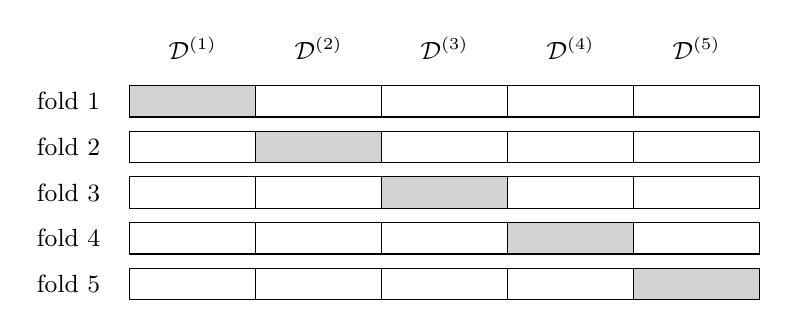
\begin{tikzpicture}[font=\small]
				\def\k{5}          % number of folds
				\def\cellw{1.6}    % width of one segment
				\def\cellh{0.40}   % height of one segment
				\def\gap{0.18}     % vertical gap between rows
				% rows: i = 1..k; columns: j = 1..k
				\foreach \i in {1,...,\k} {
					% row baseline y
					\pgfmathsetmacro{\y}{-(\i-1)*(\cellh+\gap)}
					% row label
					\node[anchor=east] at (-0.25,\y+0.5*\cellh) {fold \i};
					% draw k equal segments; shade the \i-th as validation
					\foreach \j in {1,...,\k} {
						\pgfmathsetmacro{\x}{(\j-1)*\cellw}
						\ifnum\i=\j
						\fill[gray!35] (\x,\y) rectangle ++(\cellw,\cellh);
						\draw (\x,\y) rectangle ++(\cellw,\cellh);
						\else
						\draw (\x,\y) rectangle ++(\cellw,\cellh);
						\fi
					}
				}
				% add labels D^{(j)} above the columns
				\foreach \j in {1,...,\k} {
					\pgfmathsetmacro{\x}{(\j-1)*\cellw + 0.5*\cellw}
					\node[anchor=south] at (\x,\cellh+0.2) {$\mathcal{D}^{(\j)}$};
				}
			\end{tikzpicture}
		\caption{In $k$-fold CV, the available dataset $\mathcal{D}$ is 
			evenly divided into $k$ folds $\mathcal{D}^{(1)},\,\ldots,\,\mathcal{D}^{(k)}$. Each fold is used once as a 
			validation set, while the remaining $k-1$ folds form the training set.		
			\label{fig_kfoldcv_dict}}
		\end{figure} 
		For each fold $b= 1, \,\ldots, \,k$, we train the model on the 
		union of all folds except $\mathcal{D}^{(b)}$ and validate it on 
		$\mathcal{D}^{(b)}$. The overall performance is obtained by averaging 
		the validation results across all $k$ folds.
		\\
		See also: validation, validation error.},
	first={$k$-fold cross-validation ($k$-fold CV)},
	text={$k$-fold CV} 
}

\newglossaryentry{loo}
{name={leave-one-out cross-validation (LOO-CV)},
	description={LOO-CV is a special case\index{leave-one-out cross-validation (LOO-CV)} 
		of $k$-fold cross-validation ($k$-fold CV) where the validation set is of size one, i.e., a single data point. 
		\\
		% Error 
		See also: $k$-fold cross-validation ($k$-fold CV), validation, validation error.},
	first={leave-one-out cross-validation (LOO-CV)},
	text={LOO-CV}
}

\newglossaryentry{nestedcv}
{name={nested cross-validation (nested CV)},
	description={Nested CV\index{nested cross-validation (nested CV)} is a method 
		of extending the $k$-fold cross-validation ($k$-fold CV) from training and validation sets to also cover the test set. 
		Instead of simply choosing a single test set from the data, two loops are run, i.e., 
		the outer and the inner loop. The outer loop uses $k$-fold cross-validation ($k$-fold CV) to separate a test set 
		from the data, and the inner loop again uses $k$-fold cross-validation ($k$-fold CV) to separate the remaining data 
		into training and validation sets. Doing this decreases the variance and bias in the results. 
		\\
		% Todo: Figure pending
		% Todo: Changing k-folds to k-fold and n-fold.
		See also: $k$-fold cross-validation ($k$-fold CV), leave-one-out cross-validation (LOO-CV), validation, validation error.},
	first={nested cross-validation (nested CV)},
	text={nested CV},
	firstplural={nested cross-validations (nested CVs)},
	plural={nested CVs}
}

\newglossaryentry{spectrogram}
{name={spectrogram},
	description={A\index{spectrogram} spectrogram represents the time-frequency distribution of the energy of a time signal $x(t)$.  
		Intuitively, it quantifies the amount of signal energy present within a specific time segment 
		$[t_{1},t_{2}] \subseteq \mathbb{R}$ and frequency interval $[f_{1},f_{2}]\subseteq \mathbb{R}$. 
		Formally, the spectrogram of a signal is defined as the squared magnitude of its 
		short-time Fourier transform (STFT) \cite{cohen1995time}.
        		Fig. \ref{fig:spectrogram_dict} depicts a time signal along with its spectrogram. 
		\begin{figure}[H]
			\centering
			\includegraphics[width=0.8\textwidth]{assets/spectrogram.png}
			\begin{minipage}{\textwidth}
				\vspace{3ex}
				\centering
				{\selectfont (a) \hspace{10em} (b)}
			\end{minipage}
			\caption{(a) A time signal consisting of two modulated Gaussian pulses. (b) An intensity 
			plot of the spectrogram.
			\label{fig:spectrogram_dict}}
		\end{figure}
        		The intensity plot of its spectrogram can serve as an image of a signal. A 
		simple recipe for audio signal classification is to feed this signal image 
		into deep nets originally developed for image classification and object detection \cite{Li:2022aa}. 
		It is worth noting that, beyond the spectrogram, several alternative representations exist 
		for the time-frequency distribution of signal energy \cite{TimeFrequencyAnalysisBoashash}, \cite{MallatBook}.
					\\ 
		See also: classification, deep net.}, 
	first={spectrogram},
	text={spectrogram} 
}

\newglossaryentry{graphclustering}
{name={graph clustering},
	description={Graph clustering\index{graph clustering} aims to 
		cluster data points that are represented as the nodes 
		of a graph $\mathcal{G}$. The edges of $\mathcal{G}$ represent 
		pairwise similarities between data points. We can sometimes
		quantify the extent of these similarities by an edge weight \cite{FlowSpecClustering2021}, \cite{Luxburg2007}.
					\\ 
		See also: graph, clustering, data point, edge weight. }, 
	first={graph clustering},
	text={graph clustering} 
}

\newglossaryentry{specclustering}
{name={spectral clustering},
	description={Spectral clustering\index{spectral clustering} is a particular instance of 
		graph clustering, i.e., it clusters data points 
		represented as the nodes $i=1, \,\ldots, \,n$ of a graph $\mathcal{G}$. 
		Spectral clustering uses the eigenvectors of the Laplacian matrix ${\bf L}^{(\mathcal{G})}$ 
		to construct feature vectors ${\bf x}^{(i)} \in \mathbb{R}^{d}$ 
		for each node (i.e., for each data point) $i=1, \,\ldots, \,n$. We can feed these feature vectors 
		into Euclidean space-based clustering methods, such as $k$-means 
		or soft clustering via Gaussian mixture model (GMM). Roughly speaking, the feature vectors of nodes 
		belonging to a well-connected subset (or cluster) of nodes in $\mathcal{G}$ are located 
		nearby in the Euclidean space $\mathbb{R}^{d}$ (see Fig. \ref{fig_lap_mtx_specclustering_dict}). 
		\begin{figure}[H]
			\begin{center}
				\begin{minipage}{0.4\textwidth}
			\begin{tikzpicture}
				% Define the style for filled nodes
				\begin{scope}[every node/.style={circle, fill=black, inner sep=0pt, minimum size=0.3cm}]
					% Define nodes
					\node (1) at (0,0) {};
					\node (2) [below left=of 1, xshift=-0.2cm, yshift=-1cm] {};
					\node (3) [below right=of 1, xshift=0.2cm, yshift=-1cm] {};
					\node (4) [below=of 1, yshift=0.5cm] {}; % Isolated node
				\end{scope}
				% Draw edges
				\draw (1) -- (2);
				\draw (1) -- (3);
				% Add labels (separate from filled nodes)
				\node[above=0.2cm] at (1) {$i=1$};
				\node[left=0.3cm] at (2) {$2$};
				\node[right=0.3cm] at (3) {$3$};
				\node[below=0.2cm] at (4) {$4$};
				\node at (0,-4) {(a)};
			\end{tikzpicture}
				\end{minipage} 
				\hspace*{5mm}
				\begin{minipage}{0.4\textwidth}
					\begin{equation} 
						{\bf L}^{(\mathcal{G})}\!=\!
						\begin{pmatrix} 
							2 & -1 & -1 & 0 \\ 
							-1 & 1 & 0 & 0 \\  
							-1 & 0 & 1 & 0 \\ 
							0 & 0 & 0 & 0 
						\end{pmatrix}\!=\!\mathbf{V} {\bm \Lambda} \mathbf{V}\,^{T}  
						\nonumber
					\end{equation} 
					\begin{minipage}{\textwidth}
						\vspace{3ex}
						\centering
						{\selectfont (b)}
					\end{minipage}
				\end{minipage}
				\vspace*{20mm}\\
				\begin{minipage}{0.4\textwidth}
			\begin{tikzpicture}[scale=3]
%					% Axes
					\draw[->] (-0.2, 0) -- (1.2, 0) node[right] {$v^{(1)}_{i}$};
					\draw[->] (0, -0.2) -- (0, 1.2) node[above] {$v^{(2)}_{i}$};
%					
%					% Tailored tick marks and labels
%					\draw (0,0) node[below left] {$0$};
%					\draw (1/sqrt(3), 0) node[below] {$\frac{1}{\sqrt{3}}$} -- ++(0,0.05);
%					\draw (0, 1) node[left] {$1$} -- ++(0.05,0);
%					
%					Data points
					\filldraw[blue] (0.577, 0) circle (0.03cm) node[above right] {$i=1,2,3$};
					\filldraw[blue] (0.577, 0) circle (0.03cm); % Second point overlaps
					\filldraw[blue] (0.577, 0) circle (0.03cm); % Third point overlaps
					\filldraw[red] (0, 1) circle (0.03cm) node[above right] {$4$};
%					% Grid for reference
%					\draw[dashed, gray] (1/sqrt(3), 0) -- (1/sqrt(3), 1);
%					\draw[dashed, gray] (0, 1) -- (1, 1);
					\node at (0.5,-0.5) {(c)};
			\end{tikzpicture}
				\end{minipage} 
    				\begin{minipage}{0.4\textwidth}
					\begin{align}
					& \mathbf{V} = \big( {\bf v}^{(1)},{\bf v}^{(2)},{\bf v}^{(3)},{\bf v}^{(4)} \big) \nonumber \\
					&	\mathbf{v}^{(1)}\!=\!\frac{1}{\sqrt{3}} \begin{pmatrix} 1 \\ 1 \\ 1 \\ 0 \end{pmatrix}, \,
					\mathbf{v}^{(2)}\!=\!\begin{pmatrix} 0 \\ 0 \\ 0 \\ 1 \end{pmatrix} \nonumber 
					\end{align}
					\begin{minipage}{\textwidth}
						\vspace{3ex}
						\centering
						{\selectfont (d)}
					\end{minipage}
				\end{minipage} 
				\caption{\label{fig_lap_mtx_specclustering_dict} (a) An undirected graph 
					$\mathcal{G}$ with four nodes $i=1,\,2,\,3,\,4$, each representing a data point. (b) The Laplacian matrix 
					${\bf L}^{(\mathcal{G})} \in \mathbb{R}^{4 \times 4}$ and its eigenvalue decomposition (EVD). 
					(c) A scatterplot of data points using the feature vectors 
					${\bf x}^{(i)} = \big( v^{(1)}_{i},v^{(2)}_{i} \big)\,^{T}$. 
					(d) Two eigenvectors ${\bf v}^{(1)},{\bf v}^{(2)} \in \mathbb{R}^{d}$ 
					corresponding to the eigenvalue $\lambda=0$ of the Laplacian matrix ${\bf L}^{(\mathcal{G})}$. } 
			\end{center}
		\end{figure}
		See also: clustering, graph clustering, Laplacian matrix, eigenvalue.}, 
	first={spectral clustering},
	text={spectral clustering} 
}

\newglossaryentry{flowbasedclustering}
{name={flow-based clustering},
	description={Flow-based clustering\index{flow-based clustering} groups the nodes 
		of an undirected graph by applying $k$-means clustering to nodewise 
		feature vectors. These feature vectors are built from network flows between 
		carefully selected sources and destination nodes \cite{FlowSpecClustering2021}. 
					\\ 
		See also: clustering, graph, $k$-means, feature vector.}, 
	first={flow-based clustering},
	text={flow-based clustering} 
}

\newglossaryentry{esterr}
{name={estimation error},
	description={Consider\index{estimation error} data points, each with feature vector ${\bf x}$ and label 
		$y$. In some applications, we can model the relation between the feature vector and the label
		of a data point as $y= \bar{h}({\bf x}) + \varepsilon$. Here, we 
		use some true underlying hypothesis $\bar{h}$ and a noise term $\varepsilon$, 
		which summarizes any modeling or labeling errors. The estimation error incurred by an machine learning (ML) 
		method that learns a hypothesis $\widehat{h}$, e.g., using empirical risk minimization (ERM), is defined as 
		$\widehat{h}({\bf x}) - \bar{h}({\bf x})$ for some feature vector. 
		For a parametric hypothesis space, which consists of hypothesis maps determined by 
		model parameters ${\bf w}$, we can define the estimation error as 
		$\Delta {\bf w}= \widehat{{\bf w}} - \overline{{\bf w}}$ \cite{hastie01statisticallearning}, \cite{kay}.
					\\ 
		See also: data point, feature vector, label, hypothesis, machine learning (ML), empirical risk minimization (ERM), hypothesis space, map, model parameter.},
	first={estimation error},
	text={estimation error} 
}

\newglossaryentry{dob}
{name={degree of belonging}, 
	description={Degree of belonging\index{degree of belonging} is a number that indicates the extent to which a data point 
		belongs to a cluster \cite[Ch. 8]{MLBasics}. The degree of belonging can be 
		interpreted as a soft cluster assignment. Soft clustering methods can 
		encode the degree of belonging with a real number in the interval $[0,1]$. 
		Hard clustering is obtained as the extreme case when the degree of belonging 
		only takes on values $0$ or $1$.
					\\ 
		See also: data point, cluster, soft clustering, hard clustering.}, 
	first={degree of belonging},
	firstplural={degrees of belonging},
	plural={degrees of belonging},
	text={degree of belonging} 
}

\newglossaryentry{msee}
{name={mean squared estimation error (MSEE)},
	description={Consider\index{mean squared estimation error (MSEE)} an machine learning (ML) method that 
		learns model parameters $\widehat{{\bf w}}$ based on some dataset $\mathcal{D}$. 
		If we interpret the data points in $\mathcal{D}$ as independent and identically distributed (i.i.d.) realizations of an random variable (RV) ${\bf z}$, 
		we define the estimation error $\Delta {\bf w}:=\widehat{w} - \overline{{\bf w}}$. 
		Here, $\overline{{\bf w}}$ denotes the true model parameters of the probability distribution 
		of ${\bf z}$. The MSEE is 
		defined as the expectation $\mathbb{E} \big\{ \big\| \Delta {\bf w}\big\|^{2} \big\}$ of the 
		squared Euclidean norm of the estimation error \cite{LC}, \cite{kay}.
					\\ 
		See also: random variable (RV), estimation error, probabilistic model, squared error loss.},
	first={mean squared estimation error (MSEE)},
	text={MSEE} 
}

\newglossaryentry{gtvmin}
{name={generalized total variation minimization (GTVMin)},
	description={GTVMin\index{generalized total variation minimization (GTVMin)} is an instance of regularized empirical risk minimization (RERM) 
		using the generalized total variation (GTV) of local model parameters as a regularizer \cite{ClusteredFLTVMinTSP}.
					\\ 
		See also: regularized empirical risk minimization (RERM), generalized total variation (GTV), regularizer.},
	first={generalized total variation minimization (GTVMin)},
	text={GTVMin} 
}

\newglossaryentry{networklasso}
{name={network Lasso},
	description={The network Lasso\index{network Lasso} is a special case of 
		generalized total variation minimization (GTVMin), obtained by using a norm-based discrepancy 
		measure for comparing local model parameters \cite{NetworkLasso}. 
		It can also be viewed as a generalization of the Lasso 
		method to datasets and models with an intrinsic network 
		structure.
			\\
		See also: Lasso, generalized total variation minimization (GTVMin), generalized total variation (GTV), regularized empirical risk minimization (RERM), regularizer.},
	first={network Lasso},
	text={network Lasso}
}

\newglossaryentry{regression}
{name={regression},
	description={Regression\index{regression} problems revolve around the 
		prediction of a numeric label solely from the features of a data point \cite[Ch. 2]{MLBasics}.
					\\ 
		See also: prediction, label, feature, data point.},
	first={regression},
	text={regression} 
}

\newglossaryentry{acc}
{name={accuracy},
	description={Consider\index{accuracy} data points characterized by features ${\bf x}\in \mathcal{X}$ and 
		a categorical label $y$ that takes on values from a finite label space $\mathcal{Y}$. The 
		accuracy of a hypothesis $h: \mathcal{X}\rightarrow \mathcal{Y}$, when applied to the data points in a dataset 
		$\mathcal{D}= \big\{ \big({\bf x}^{(1)}, y^{(1)} \big), \,\ldots, \,\big({\bf x}^{(m)},y^{(m)}\big) \big\}$, 
		is then defined as $1 - (1/m)\sum_{r=1}^{m} L^{(0/1)}\left(\big({\bf x}^{(r)},y^{(r)}\big),h\right)$ 
		using the $0/1$ loss $L^{(0/1)}\left(\cdot,\cdot \right)$.
					\\ 
		See also: $0/1$ loss, loss, metric.},
	first={accuracy},
	text={accuracy} 
}

\newglossaryentry{expert}
{name={expert},
	description={machine learning (ML)\index{expert} aims to learn a hypothesis $h$ that accurately predicts the label 
		of a data point based on its features. We measure the prediction error using 
		some loss function. Ideally, we want to find a hypothesis that incurs minimal loss 
		on any data point. We can make this informal goal precise via the independent and identically distributed assumption (i.i.d.\ assumption) 
		and by using the Bayes risk as the baseline for the (average) loss of a hypothesis. 
		An alternative approach to obtaining a baseline is to use the hypothesis $h'$ learned 
		by an existing machine learning (ML) method. We refer to this hypothesis $h'$ as an expert \cite{PredictionLearningGames}. 
		Regret minimization methods learn a hypothesis
		that incurs a loss comparable to that of the best expert \cite{PredictionLearningGames}, \cite{HazanOCO}.
					\\ 
		See also: loss function, baseline, regret.},
	first={expert},
	text={expert} 
}

\newglossaryentry{nfl}
{name={networked federated learning (NFL)},
	description={NFL\index{networked federated learning (NFL)} refers 
		to methods that learn personalized models in a distributed fashion. These methods learn from local datasets 
		that are related by an intrinsic network structure.
					\\ 
		See also: model, local dataset, federated learning (FL).},
	first={networked federated learning (NFL)},
	text={NFL} 
}

\newglossaryentry{fedprox}
{name={federated proximal (FedProx)},
	description={FedProx\index{federated proximal (FedProx)} refers to an iterative federated learning (FL) algorithm that alternates between separately 
		training local models and combining the updated local model parameters. In contrast to federated averaging (FedAvg), which uses 
		stochastic gradient descent (SGD) to train local models, FedProx uses a proximal operator for the training \cite{FedProx2020}.
					\\ 
		See also: federated learning (FL), algorithm, local model, model parameter, federated averaging (FedAvg), stochastic gradient descent (SGD), proximal operator.}, 
	first={FedProx}, 
	text={FedProx} 
}

\newglossaryentry{relu}
{name={rectified linear unit (ReLU)},
	description={The\index{rectified linear unit (ReLU)} ReLU is 
		a popular choice for the activation function of a neuron within an artificial neural network (ANN). It is defined 
		as $\sigma(z) = \max\{0,z\}$, with $z$ being the weighted input of the artificial 
		neuron.
					\\ 
		See also: activation function, artificial neural network (ANN).}, 
	first={rectified linear unit (ReLU)}, 
	text={ReLU} 
}

\newglossaryentry{hypothesis}
{name={hypothesis},
	description={A\index{hypothesis} hypothesis refers to a map (or function) $h: \mathcal{X}\rightarrow \mathcal{Y}$ 
		from the feature space $\mathcal{X}$ to the label space $\mathcal{Y}$. 
		Given a data point with features ${\bf x}$, we use a hypothesis 
		map $h$ to estimate (or approximate) the label $y$ 
		using the prediction $\hat{y} = h({\bf x})$. 
		\begin{figure}[H]
		\centering
			\begin{tikzpicture}[
 		  	>=Latex, node distance=2.0cm,
 		  	box/.style={draw, rounded corners=2pt, inner sep=6pt},
  		 	label/.style={font=\footnotesize},
  		 	thinline/.style={line width=0.6pt}
		 	]
			% % --- Input: audio signal ---
		 	\node[minimum width=3.8cm, minimum height=1.6cm] (audio) {};
		 	%\node[label, above=1mm of audio] {$\mathcal{X}$};
		 	\node[label] at (audio.north) [yshift=0mm] {audio samples ${\bf x}\in \mathbb{R}^{d}$};
			% % A tiny waveform inside the audio box
		 	\begin{scope}
		 	%\clip (audio.south west) ++(0.15,0.15) rectangle ($(audio.north east)+(-0.15,-0.15)$);
		 	\draw[thinline]
		 		($(audio.west)+(0.2,0)$) .. controls +(.3,.35) and +(-.3,.35) .. ++(0.8,0)
		 		.. controls +(.3,-.35) and +(-.3,-.35) .. ++(0.8,0)
		 		.. controls +(.3,.25) and +(-.3,.25) .. ++(0.8,0)
		 		.. controls +(.3,-.25) and +(-.3,-.25) .. ++(0.8,0);
		 	\end{scope}
			% % --- Hypothesis map ---
		 	\node[box,right=1.0cm of audio, minimum width=2.2cm, minimum height=1.6cm] (model)
		 	{$h$};
		 	\draw[->,thinline] (audio) -- (model) ; %node[midway,above,label] {features \& inference};
			% % --- Output: rating bar ---
		 	\node[right=1.0cm of model, minimum width=3.2cm, minimum height=1.6cm] (rating) {};
		 	\node[label, align=center] at ($(rating.north)+(0,-6mm)$)
		 		{};
			% % Draw a minimalist horizontal score bar
		 	\coordinate (barL) at ($(rating.west)+(0.4,0)$);
		 	\coordinate (barR) at ($(rating.east)+(-0.4,0)$);
		 	\def\score{0.82}
		 	\coordinate (ptr) at ($(barL)!{\score}!(barR)$);
		 	%\draw[thinline] (ptr) -- ++(0,-0.28);
			%\fill (ptr) circle (1.2pt);
		 	\node[label, above=0pt of ptr] {$h({\bf x})=0.82 (\approx \mbox{Freddie level})$};
		 	\draw[->,thinline] (model) -- (rating);
		 	\end{tikzpicture}
		\caption{\label{fig:hypothesis_dict} A hypothesis $h: \mathcal{X}\rightarrow \mathcal{Y}$ maps the features 
			${\bf x}\in \mathcal{X}$ of a data point to a prediction $h({\bf x}) \in \mathcal{Y}$ of the label. 
			For example, the machine learning (ML) application \url{https://freddiemeter.withyoutube.com/} uses the samples of an audio 
			recording as features to predict how closely a person’s singing resembles that of Freddie Mercury. }
		\end{figure}
		Machine learning (ML) is all about learning (or finding) a hypothesis map $h$ 
		such that $y\approx h({\bf x})$ for any data point 
		(with features ${\bf x}$ and label $y$). Practical machine learning (ML) methods, 
		limited by finite computational resources, must restrict learning to a subset of all possible 
		hypothesis maps. This subset is called the hypothesis space or simply the model underlying 
		the method.
					\\ 
		See also: map, function, prediction, model.},
	first={hypothesis},
	firstplural={hypotheses},
	plural={hypotheses},
	text={hypothesis}  
}

\newglossaryentry{effdim}
{name={effective dimension},
	description={The\index{effective dimension} effective dimension $d_{\rm eff} \left( \mathcal{H}\right)$ of 
		an infinite hypothesis space $\mathcal{H}$ is a measure of its size. Loosely speaking, the 
		effective dimension is equal to the effective number of independent tunable model parameters. 
		These parameters might be the coefficients used in a linear map or the 
		weights and bias terms of an artificial neural network (ANN).
					\\ 
		See also: hypothesis space, model parameter, artificial neural network (ANN).},
	first={effective dimension},
	text={effective dimension}  
}

\newglossaryentry{labelspace}
{name={label space},
	description={In an machine learning (ML) application\index{label space}, each data point is described by a 
		set of features together with an associated label. 
		The set of all admissible label values is called the label space,
		denoted by $\mathcal{Y}$. Importantly, $\mathcal{Y}$ may include values that no 
		observed data point has as its label value. 
		To a large extent, the choice of $\mathcal{Y}$ is up to the machine learning (ML) engineer 
		and depends on the problem formulation. Fig.~\ref{fig_label_spaces_dict} shows some examples 
		of label spaces that are commonly used in machine learning (ML) applications.
		\begin{figure}[H]
		\centering
		\begin{tikzpicture}[>=Stealth, font=\small]
			% (a) Real line for regression
			\begin{scope}[shift={(0,0)}]
				\draw[->] (-2,0) -- (2,0);
				\node[below=6pt] at (0,-0.7) {$\mathcal{Y}\!=\!\mathbb{R}$ (regression)};
				\node at (0,-2) {(a)};
			\end{scope}
			% (b) Plane for multi-label regression
			\begin{scope}[shift={(7,0)}]
				% shaded rectangle
				\fill[gray!20] (-1,-0.5) rectangle (1,0.5);
				\draw[->] (-2,0) -- (2,0);
				\draw[->] (0,-1) -- (0,1);
				\node[below=6pt] at (0,-0.7) {$\mathcal{Y}\!=\!\mathbb{R}^{2}$ (multi-label regression)};
				\node at (0,-2) {(b)};
			\end{scope}
			% (c) Binary classification
			\begin{scope}[shift={(0,-3)}]
				\fill (-1,0) circle (1.2pt) node[below=2pt] {\text{``hot''}};
				\fill ( 1,0) circle (1.2pt) node[below=2pt] {\text{``cold''}};
				\node[below=14pt] at (0,-0.7) {$|\mathcal{Y}|=2$ (binary classification)};
				\node at (0,-2.3) {(c)};
			\end{scope}
			% (d) Ordinal regression: directed chain
			\begin{scope}[shift={(7,-3)}]
				\node[circle, inner sep=1pt, draw] (n1) at (-1.5,0) {};
				\node[circle, inner sep=1pt, draw] (n2) at (-0.5,0) {};
				\node[circle, inner sep=1pt, draw] (n3) at ( 0.5,0) {};
				\node[circle, inner sep=1pt, draw] (n4) at ( 1.5,0) {};
				\draw[->] (n1) -- (n2);
				\draw[->] (n2) -- (n3);
				\draw[->] (n3) -- (n4);
				\node[below=2pt of n1] {1};
				\node[below=2pt of n2] {2};
				\node[below=2pt of n3] {3};
				\node[below=2pt of n4] {4};
				\node[below=14pt] at (0,-0.7) {$\mathcal{Y}\!=\!\{1,\,2,\,3,\,4\}$ (ordinal regression)};
				\node at (0,-2.3) {(d)};
			\end{scope}
		\end{tikzpicture}
		\caption{\label{fig_label_spaces_dict} Examples of label spaces and the corresponding types of machine learning (ML).
			(a) Regression. (b) Multi-label regression. (c) Binary classification. (d) Ordinal regression.}
		\end{figure}
		The choice of the label space $\mathcal{Y}$ determines the type of machine learning (ML) methods 
		appropriate for the application at hand. Regression methods use the $\mathcal{Y}= \mathbb{R}$, 
		while binary classification methods use a label space $\mathcal{Y}$ that consists of two different 
		elements, i.e., $|\mathcal{Y}|=2$. Ordinal regression methods use a finite, ordered set of 
		label values, e.g., $\mathcal{Y}= \{1,\,2,\,3,\,4\}$ with the natural ordering $1 < 2 < 3 < 4$. 
					\\ 
		See also:  data point, label, regression, classification.}, 
	first={label space},
	text={label space}  
}

\newglossaryentry{prediction}
{name={prediction},
	description={A\index{prediction} prediction is an estimate or approximation for some 
		quantity of interest. Machine learning (ML) revolves around learning or finding a hypothesis map $h$ 
		that reads in the features ${\bf x}$ of a data point and delivers a prediction 
		$\widehat{y} :=h({\bf x})$ for its label $y$.
					\\ 
		See also: machine learning (ML), hypothesis, map, feature, data point, label.},
	first={prediction},
	plural={predictions},
	text={prediction}  
}

\newglossaryentry{histogram}
{name={histogram},
	description={Consider\index{histogram} a dataset $\mathcal{D}$ that consists of 
		$m$ data points ${\bf z}^{(1)}, \,\ldots, \,{\bf z}^{(m)}$, 
		each of them belonging to some cell $[-U,U] \times \ldots \times [-U,U] \subseteq \mathbb{R}^{d}$ with side 
		length $U$. We partition this cell evenly into smaller elementary cells with side 
		length $\Delta$. The histogram of $\mathcal{D}$ assigns each elementary cell to 
		the corresponding fraction of data points in $\mathcal{D}$ that fall into this 
		elementary cell. A visual example of such a histogram is provided in Fig. \ref{fig:histogram_dict}.
		\begin{figure}[H]
		\centering
		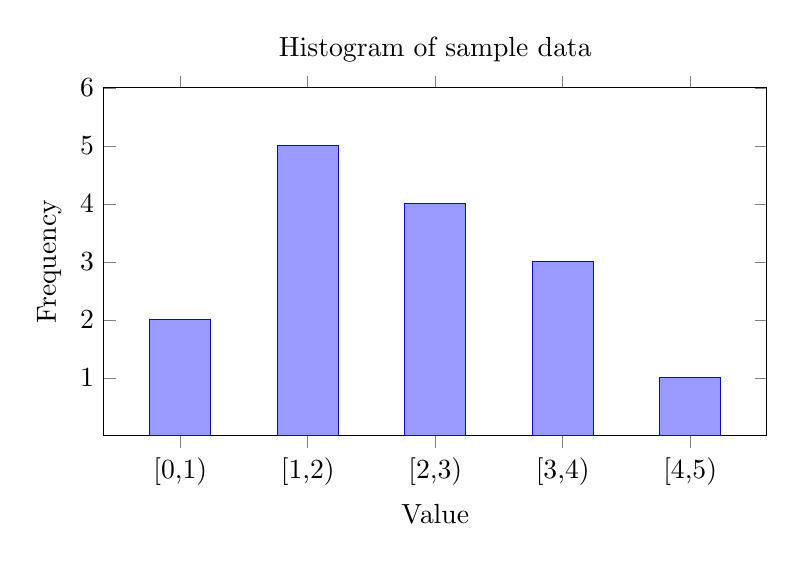
\begin{tikzpicture}
		\pgfplotsset{compat=1.18}
		\begin{axis}[
		    ybar,
		    ymin=0,
		    ymax=6,
		    bar width=22pt,
		    width=10cm,
		    height=6cm,
		    xlabel={Value},
		    ylabel={Frequency},
		    ytick={1,2,3,4,5,6},
		    xtick={1,2,3,4,5},
		    xticklabels={{[0,1)}, {[1,2)}, {[2,3)}, {[3,4)}, {[4,5)}},
		    enlarge x limits=0.15,
		    title={Histogram of sample data}
			]
		\addplot+[fill=blue!40] coordinates {(1,2) (2,5) (3,4) (4,3) (5,1)};
		\end{axis}
		\end{tikzpicture}
		\caption{A histogram consists of the fractions of data points that 
			fall within different value ranges (i.e., bins). Each bar height shows 
			the count of samples in the corresponding interval.}
			\label{fig:histogram_dict}
		\end{figure}
		See also: dataset, data point, sample.},
	first={histogram},
	text={histogram}  
}

\newglossaryentry{bootstrap}
{name={bootstrap},
	description={For\index{bootstrap} the analysis of machine learning (ML) methods, it is often 
	    	useful to interpret a given dataset $\mathcal{D}= \big\{ {\bf z}^{(1)}, \,\ldots, \,{\bf z}^{(m)}\big\}$ 
		as a collection of (realizations of) independent and identically distributed (i.i.d.) random variables (RVs) with 
		common probability distribution $\mathbb{P}$. In practice, the probability distribution $\mathbb{P}$ 
		is unknown and must be estimated from $\mathcal{D}$. The idea of the bootstrap 
		method is to use the empirical distribution $\mathbb{P}^{(\mathcal{D})}$ 
		of $\mathcal{D}$ as an estimator for $\mathbb{P}$ \cite{hastie01statisticallearning}:
		$$ \frac{1}{m} \big| r: {\bf z}^{(r)} \in \mathcal{A} \big| \approx \mathbb{P}\left(\mathcal{A}\right).$$
		Repeatedly sampling from the empirical distribution, which is equivalent 
		to sampling with replacement from $\mathcal{D}$ \cite{BoostrapBook}, 
		results in new datasets $\mathcal{D}^{(1)}, \,\ldots, \,\mathcal{D}^{(B)}$, each containing 
		$m$ data points. We then use each of 
		those datasets for model training (e.g., via empirical risk minimization (ERM)), 
		resulting in the learned hypotheses
		$\widehat{h}^{(1)}, \,\ldots, \,\hat{h}^{(B)}.$ 
        		We can use these learned hypotheses to estimate important characteristics 
		of an machine learning (ML) method such as bias, variance, or generalization gap \cite{hastie01statisticallearning}.
		\\
		See also: independent and identically distributed (i.i.d.), random variable (RV), probability distribution, histogram.},
	first={bootstrap},
	text={bootstrap}  
}

\newglossaryentry{featurespace}
{name={feature space},
	description={The\index{feature space} feature space of a given machine learning (ML) application 
		or method is constituted by all potential values that the feature vector of a data point can take on. 
		For data points described by a fixed number $d$ of numerical features, 
		a common choice for the feature space is the Euclidean space $\mathbb{R}^{d}$. 
		However, the mere presence of $d$ numeric features does not imply that $\mathbb{R}^{d}$ 
		is the most appropriate representation of the feature space. Indeed, the numerical features  
		might be assigned to data points in a largely arbitrary or random manner, resulting 
		in data points that are randomly scattered throughout $\mathbb{R}^{d}$ 
		without any meaningful geometric structure. Feature learning methods try to learn a 
		transformation of the original (potentially nonnumeric) features to ensure a 
		more meaningful arrangement of data points in $\mathbb{R}^{d}$. 
		Three examples of feature spaces are shown in Fig. \ref{fig_featurespace_dict}.
		\begin{figure}[H]
			\centering
			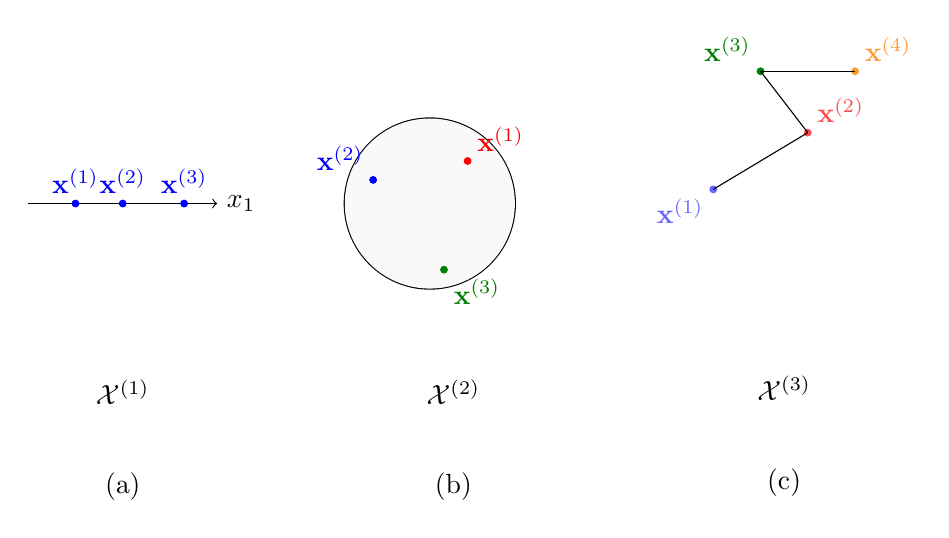
\begin{tikzpicture}[scale=0.6]
			% --------- 1D Line Feature Space (left) ---------
			\begin{scope}[xshift=0cm]
  				% Axis
 	 			\draw[->] (-0.5, 0) -- (3.5, 0) node[right] {$x_1$};
  				% Points
  				\foreach \x/\lbl in {0.5/${\bf x}^{(1)}$, 1.5/${\bf x}^{(2)}$, 2.8/${\bf x}^{(3)}$}
    				\filldraw[blue] (\x,0) circle (2pt) node[above] {\lbl};
  				% Label
  				\node at (1.5, -4.0)  {$\mathcal{X}^{(1)}$};
				\node at (1.5, -6) {(a)};
			\end{scope}
			% --------- 2-D Bounded (Disk) Feature Space (middle) ---------
			\begin{scope}[xshift=8cm]
  				% Circle boundary
  				\draw[thick] (0,0) circle (1.8);
  				\fill[gray!5] (0,0) circle (1.8);
  				% Points inside circle
  				\filldraw[red] (0.8, 0.9) circle (2pt) node[anchor=south west] {${\bf x}^{(1)}$};
  				\filldraw[blue] (-1.2, 0.5) circle (2pt) node[anchor=south east] {${\bf x}^{(2)}$};
  				\filldraw[green!50!black] (0.3, -1.4) circle (2pt) node[anchor=north west] {${\bf x}^{(3)}$};
  				% Label
  				\node at (0.5, -4) {$\mathcal{X}^{(2)}$};
				\node at (0.5, -6) {(b)};
			\end{scope}
			% --------- Graph-Based Feature Space (right) ---------
			\begin{scope}[xshift=14cm, yshift=0.3cm]
  				% Nodes
 	 			\filldraw[blue!60] (0,0) circle (2pt) node[anchor=north east] {${\bf x}^{(1)}$};
 	 			\filldraw[red!70] (2,1.2) circle (2pt) node[anchor=south west] {${\bf x}^{(2)}$};
  				\filldraw[green!50!black] (1,2.5) circle (2pt) node[anchor=south east] {${\bf x}^{(3)}$};
  				\filldraw[orange!80] (3,2.5) circle (2pt) node[anchor=south west] {${\bf x}^{(4)}$};
  				% Edges
  				\draw[-] (0,0) -- (2,1.2);
  				\draw[-] (2,1.2) -- (1,2.5);
  				\draw[-] (1,2.5) -- (3,2.5);
  				% Label
  				\node at (1.5, -4.2) {$\mathcal{X}^{(3)}$};
				\node at (1.5, -6.2) {(c)};
			\end{scope}
			\end{tikzpicture}
		\caption{Three different feature spaces. (a) A linear space $\mathcal{X}^{(1)} = \mathbb{R}$. (b) A 
			bounded convex set $\mathcal{X}^{(2)} \subseteq \mathbb{R}^{2}$. (c) A discrete space 
			$\mathcal{X}^{(3)}$ whose elements are nodes of an undirected graph. \label{fig_featurespace_dict}}
		\end{figure}
		See also: feature vector, Euclidean space.},
	first={feature space},
	text={feature space}  
}

\newglossaryentry{missingdata}
{name={missing data},
	description={Consider\index{missing data} a dataset constituted by data points collected via 
		some physical device. Due to imperfections and failures, some of the feature 
		or label values of data points might be corrupted or simply missing. 
		Data imputation aims to estimate these missing values \cite{Abayomi2008DiagnosticsFM}. 
		We can interpret data imputation as an machine learning (ML) problem where the label of a data point is 
		the value of the corrupted feature.
				\\
		See also: feature, label. },
	first={missing data},
	text={missing data}  
}

\newglossaryentry{hyperparameter}
{name={hyperparameter},
	description={A hyperparameter\index{hyperparameter} associated with an machine learning (ML) method is 
		a quantity that is used to select among a family of models. 
		Typical examples include the learning rate used in a gradient-based method, 
		the number of features used in a linear model, or the 
		maximum depth of a decision tree. The usefulness of a specific 
		hyperparameter choice can be assessed via validation. Similar 
		to learning (or tuning) model parameters by empirical risk minimization (ERM) on a training set, 
		we can learn (or tune) hyperparameters via minimizing the validation error. Thus, 
		in a sense, hyperparameters are higher-level model parameters that are learned 
		via a higher-level form of empirical risk minimization (ERM), i.e., minimizing the validation error obtained by 
		the trained model with a given hyperparameter value. 
			\\ 
		See also: model, validation, model parameter.},
	first={hyperparameter},
	text={hyperparameter},
	plural={hyperparameters},
	firstplural={hyperparameters}
}

\newglossaryentry{dataimputation}
{name={data imputation},
	description={See\index{data imputation} missing data.},
	first={data imputation},
	text={data imputation}  
}

\newglossaryentry{feature}
{name={feature},
	description={A\index{feature} feature of a data point is one of its properties 
	    	that can be measured or computed easily without the need for human supervision. 
		For example, if a data point is a digital image (e.g., stored as a \texttt{.jpeg} file), 
		then we could use the red–green–blue (RGB) intensities of its pixels as features. 
		Another example is shown in Fig.\ \ref{fig:audio_features_dict}, where the signal 
		samples of a finite-duration audio signal are used as its features.
		\begin{figure}[H]
		\centering
		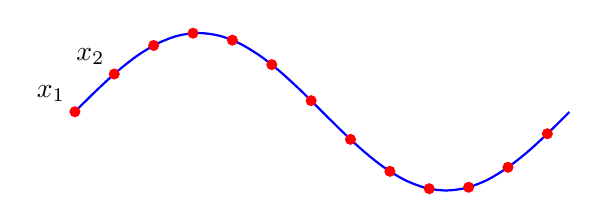
\begin{tikzpicture}[scale=1]
		% Draw a smooth waveform (sine curve as proxy for audio)
		\draw[thick, blue, domain=0:6.28, smooth, variable=\x] 
			plot ({\x}, {sin(\x r)});
		% Mark sample points at regular intervals
		\foreach \x [count=\i] in {0,0.5,...,6.28} {
			\fill[red] (\x, {sin(\x r)}) circle (2pt);
			% Label only the first two samples
			\ifnum\i=1
				\node[above left] at (\x, {sin(\x r)}) {$x_1$};
			\fi
			\ifnum\i=2
				\node[above left] at (\x, {sin(\x r)}) {$x_2$};
			\fi
		}
		\end{tikzpicture}
		\caption{An audio signal (blue waveform) and its discretized signal samples (red dots) that 
			can be used as its features $x_{1},\,\ldots,\,x_{d}$. \label{fig:audio_features_dict}}
		\end{figure}
		Domain-specific synonyms for the term feature are "covariate," "explanatory variable," 
		"independent variable," "input (variable)," "predictor (variable)," or "regressor" 
		\cite{Everitt2010}, \cite{Gujarati2021}, \cite{Dodge2003}. 
		\\
		See also: data point.}, 
	first={feature},
	plural={features},
	text={feature}  
}

\newglossaryentry{featurevec}
{name={feature vector},
	description={Feature vector refers to a\index{feature vector} vector ${\bf x}= \big(x_{1}, \,\ldots, \,x_{d}\big)\,^{T}$ 
		whose entries are individual features $x_{1}, \,\ldots, \,x_{d}$. Many machine learning (ML) methods 
		use feature vectors that belong to some finite-dimensional Euclidean space $\mathbb{R}^{d}$. 
		For some machine learning (ML) methods, however, it can be more convenient to work with feature 
		vectors that belong to an infinite-dimensional vector space (e.g., see kernel method). 
			\\
		See also: feature, vector, machine learning (ML), Euclidean space, vector space.}, 
	first={feature vector},
	plural={feature vectors},
	firstplural={feature vectors},
	text={feature vector}  
}

\newglossaryentry{label}
{name={label},
	description={A label\index{label} is a higher-level fact or quantity of interest associated 
		with a data point. For example, if the data point is an image, the label 
		could indicate whether the image contains a cat 
		\cite{Everitt2010}, \cite{Gujarati2021}, \cite{Dodge2003}.
				\\
		See also: data point, label space.},
	first={label},
	plural={labels},
	text={label}  
}

\newglossaryentry{data}
{name={data},
	description={In the context of machine learning (ML), the term 
 		data\index{data} is often used as a synonym for dataset
  		\cite{Everitt2010}, \cite{OxfordStatisticsDictionary}. 
  		The ISO/IEC 2382:2015 standard \cite{ISO2382} defines data as a \begin{quote} reinterpretable representation of 
  		information in a formalized manner suitable for communication, interpretation, or processing.\end{quote}
  		See also: dataset, data point, sample.}, 
  	first={data},
	text={data}
}

\newglossaryentry{relational model}
{name={relational model},
	description={A relational model\index{relational model} is a mathematical representation of data. 
		The core idea is to ogranize data as a collection of 
		tables (or relations) \cite{silberschatz2019database}, \cite{codd1970relational}. 
		A table consists of rows and columns, where each 
		row corresponds to a single data point, and each 
		column represents a specific attribute of a data point. 
		machine learning (ML) methods use these attributes as the features 
		and label of a data point. Table~\ref{tab:relmodel_dict} shows 
		a relational representation of a dataset that consists of cows. 
		In the relational model, the order of rows is immaterial, and each 
		attribute (i.e., column) is associated with a domain that specifies the set 
		of admissible values. 
		In machine learning (ML) applications, these attribute domains correspond to the 
		feature space and the label space.
				\begin{table}[H]
					\refstepcounter{table}
					\caption*{
						\centering 
						\scshape TABLE \thetable \\[0.5ex]
						\scshape A Relation (or Table) That Represents the dataset in Fig. \ref{fig_cows_dataset_dict} 
					}
					\label{tab:relmodel_dict} 
					\centering
					\begin{tabular}{lcccc}
						\hline
						\textbf{Name} & \textbf{Weight} & \textbf{Age} & \textbf{Height} & \textbf{Stomach temperature} \\
						\hline
						Zenzi & 100 & 4 & 100 & 25 \\
						Berta & 140 & 3 & 130 & 23 \\
						Resi  & 120 & 4 & 120 & 31 \\
						\hline
					\end{tabular}
				\end{table}
		See also: data, data point, features, label, dataset.}, 
	first={relational model},
	text={relational model}
}
  		
\newglossaryentry{tabulardata}
{name={tabular data},
	description={Tabular data\index{tabular data} consist of data points 
		that are characterized by a common set of attributes. These attributes 
		can be used as the features or labels of data points. 
		If the attributes are numeric, we can represent a dataset by 
		a data matrix $\mathbf{D} \in \mathbb{R}^{m\times d}$, 
		where each of the $m$ rows corresponds to a single data point,
		and each of the $d$ columns represents a specific attribute \cite{Everitt2022}.
		\\
		See also: data, data point. }, 
	first={tabular data},
	text={tabular data}
}

\newglossaryentry{datamatrix}
{name={data matrix},
	description={See tabular data\index{data matrix}.}, 
	first={data matrix},
	firstplural={data matrices},
	plural={data matrices},
	text={data matrix}
}
		
\newglossaryentry{dataset}
{name={dataset},
	description={A\index{dataset} dataset is a set of distinct data points. 
		Strictly speaking, a dataset is an unordered collection of data points 
		that does not contain any repetitions. However, in machine learning (ML) literature, the 
		term dataset is often used as a synonym for sample, i.e., 
		a sequence (or finite list) of data points that may contain repetitions. 
		machine learning (ML) methods use datasets for model training and validation. 
		The notion of a dataset is broad, i.e., data points may represent concrete 
		physical entities (such as humans or animals) or abstract objects (such as numbers). 
		For illustration, Fig.~\ref{fig_cows_dataset_dict} depicts a dataset whose 
		data points are cows.	
		\begin{figure}[H]
			\begin{center}
			\label{fig:cowsintheswissalps_dict}
			\includegraphics[width=0.5\textwidth]{assets/CowsAustria.jpg}
		  	\end{center}
			\caption{\label{fig_cows_dataset_dict}A cow herd somewhere in the Alps.}
	 	\end{figure}
		Quite often, an machine learning (ML) engineer does not have direct access to the underlying dataset. 
		For instance, accessing the dataset in Fig.~\ref{fig_cows_dataset_dict} would require 
		visiting the cow herd. In practice, we work with a more convenient 
		representation (or approximation) of the dataset. Various mathematical models 
		have been developed for this purpose \cite{silberschatz2019database}, \cite{abiteboul1995foundations}, 
		\cite{hoberman2009data}, \cite{ramakrishnan2002database}. One of the most widely used is 
		the relational model, which organizes data as a table (or relation) 
		\cite{silberschatz2019database}, \cite{codd1970relational}. A table consists of 
		rows and columns, where each row corresponds to a single data point, and each 
		column represents a specific attribute of a data point. 
		machine learning (ML) methods typically interpret these attributes as features 
		or as a label of a data point. As an illustration, 
		Table~\ref{tab:cowdata_dict} shows a relational representation of the 
		dataset from Fig.~\ref{fig_cows_dataset_dict}. In the relational model, 
		the order of rows is immaterial, and each attribute (i.e., column) is associated with a 
		domain that specifies the set of admissible values. In machine learning (ML) applications, 
		these attribute domains correspond to the feature space and the label space.
		\begin{table}[H]
			\refstepcounter{table}
			\caption*{
				\centering 
				\scshape TABLE \thetable \\[0.5ex]
				\scshape A Relation (or Table) That Represents the Dataset in Fig. \ref{fig_cows_dataset_dict} 
			}
			\label{tab:cowdata_dict} 
			\centering
			\begin{tabular}{lcccc}
				\hline
				\textbf{Name} & \textbf{Weight} & \textbf{Age} & \textbf{Height} & \textbf{Stomach temperature} \\
				\hline
				Zenzi & 100 & 4 & 100 & 25 \\
				Berta & 140 & 3 & 130 & 23 \\
				Resi  & 120 & 4 & 120 & 31 \\
				\hline
			\end{tabular}
		\end{table}
 		While the relational model is useful for the study of many machine learning (ML) applications, 
		it may be insufficient regarding the requirements for trustworthy artificial intelligence (trustworthy AI). Modern 
 		approaches like datasheets for datasets provide more comprehensive 
 		documentation, including details about the data collection process, intended 
 		use, and other contextual information \cite{DatasheetData2021}.
 		\\
		See also: data point, sample, data, feature, feature space, label space.},
	first={dataset},
	plural={datasets},
	text={dataset}  
}

\newglossaryentry{predictor}
{name={predictor},
	description={A\index{predictor} predictor is a real-valued hypothesis map. 
		Given a data point with features ${\bf x}$, the value 
		$h({\bf x}) \in \mathbb{R}$ is used as a prediction for the true 
		numeric label $y\in \mathbb{R}$ of the data point.
				\\
		See also: hypothesis, map, data point, feature, prediction, label. },
	first={predictor},
	text={predictor}  
}

\newglossaryentry{labeled datapoint}
{name={labeled data point},
 	description={A\index{labeled data point} data point whose label is known or has been determined 
 		by some means that might require human labor.
			\\
		See also: data point, label.},
 	first={labeled data point},
	plural={labeled data points},
	firstplural={labeled data points},
 	text={labeled data point}  
}
 
\newglossaryentry{samplespace}
{name={sample space}, 
  	description={A\index{sample space} sample space is the set of all possible 
		outcomes of a random experiment \cite{BillingsleyProbMeasure}, 
		\cite{BertsekasProb}, \cite{AshProbMeasure}, \cite{papoulis}. 
		\\
 		See also: probability space.},  
  	first={sample space}, 
 	firstplural={sample spaces},
 	plural={sample spaces},
  	text={sample space}
} 
	
\newglossaryentry{realization}
{name={realization},
	description={Consider\index{realization} an random variable (RV) ${\bf x}$ that maps each outcome 
		$\omega\in \Omega$ of a probability space to an element $a$ of a 
		measurable space $\mathcal{N}$ \cite{RudinBookPrinciplesMatheAnalysis}, \cite{BillingsleyProbMeasure}, \cite{HalmosMeasure}. 
		A realization of ${\bf x}$ is any element ${\bf a}\in \mathcal{N}$ such that there exists 
		an element $\omega' \in \Omega$ with ${\bf x}(\omega') = {\bf a}$.
			\\
		See also: random variable (RV), outcome, probability space, measurable.}, 
	first={realization},
	plural={realizations},
	text={realization}  
}

\newglossaryentry{trainset}
{name={training set},
	description={A\index{training set} training set is a dataset $\mathcal{D}$ that consists of some data points used in empirical risk minimization (ERM) 
		to learn a hypothesis $\hat{h}$. The average loss of $\hat{h}$ on the 
		training set is referred to as the training error. The comparison of the training error with the 
		validation error of $\hat{h}$ allows us to diagnose the machine learning (ML) method and informs how to improve 
		the validation error (e.g., using a different hypothesis space or collecting more data points) \cite[Sec. 6.6]{MLBasics}.
			\\
		See also: training, dataset, data point, empirical risk minimization (ERM), hypothesis, loss, training error, validation error, machine learning (ML), hypothesis space.},
	first={training set},
	plural={training sets},
	firstplural={training sets},
	text={training set}  
}

\newglossaryentry{netmodel}
{name={networked model},
 	description={A\index{networked model} networked model over an federated learning network (FL network) $\mathcal{G}= \left( \mathcal{V},\mathcal{E}\right)$ assigns 
   		a local model (i.e., a hypothesis space) to each node $i\in \mathcal{V}$ of the federated learning network (FL network) $\mathcal{G}$.
   		\\
		See also: model, federated learning network (FL network), local model, hypothesis space.}, 
   first={networked model},
   text={networked model}  
}

\newglossaryentry{batch}
{name={batch},
	description={In\index{batch} the context of stochastic gradient descent (SGD), a batch refers to a randomly 
		chosen subset of the overall training set. We use the data points in this subset 
		to estimate the gradient of training error and, in turn, to update the model parameters.
			\\
		See also: stochastic gradient descent (SGD), training set, data point, gradient, training error, model parameter.}, 
 	first={batch},
 	firstplural={batches}, 
 	plural={batches}, 
 	text={batch}  
}

\newglossaryentry{epoch}
{name={epoch},
	description={An epoch\index{epoch} represents one complete pass of the entire training set through some learning 
		algorithm. It refers to the point at which a model has processed every data point in the training set once. 
		Training a model usually requires multiple epochs, since each iteration allows the model to refine the 
		parameters and improve predictions. The number of epochs is something predefined by the user,  
		and thus a hyperparameter, which plays a crucial role in determining how the model will generalize to unseen data. 
		Too few epochs will result in underfitting, while too many epochs can result in overfitting.
		\\
		See also: training set, algorithm, model, data point, parameter, prediction, underfitting, overfitting.},
	first={epoch},
	text={epoch}
} 

\newglossaryentry{netdata}
{name={networked data},
	description={Networked\index{networked data} data consist of local datasets 
		that are related by some notion of pairwise similarity. We can represent networked 
		data using a graph whose nodes carry local datasets and whose edges encode 
		pairwise similarities. An example of networked data can be found in federated learning (FL) applications 
		where local datasets are generated by spatially distributed devices.
			\\
		See also: data, local dataset, graph, federated learning (FL), device.}, 
	first={networked data},
	text={networked data}  
}

\newglossaryentry{trainerr}
{name={training error},
	description={Training error is the\index{training error} average loss of a hypothesis when 
		predicting the labels of the data points in a training set. 
		We sometimes also refer to training error as the minimal average loss 
		that is achieved by a solution of empirical risk minimization (ERM).
				\\
		See also: loss, hypothesis, label, data point, training set, empirical risk minimization (ERM).},
	first={training error},
	text={training error}  
}

\newglossaryentry{datapoint}
{name={data point},
	description={A\index{data point} data point is any object that conveys information~\cite{coverthomas}. 
		Examples include students, radio signals, trees, images, random variables (RVs), real numbers, 
 		or proteins. We describe data points of the same type by two categories 
		of properties. The first category includes features that are measurable or 
		computable properties of a data point. These attributes can be automatically extracted 
		or computed using sensors, computers, or other data collection systems. For a data 
		point that represents a patient, one feature could be the body weight.
		The second category includes labels that are higher level facts (or quantities of interest)—that is, 
		facts that typically require human expertise or domain knowledge to determine rather than being directly 
		measurable—associated with the data point. For a data point that represents a patient, 
		a cancer diagnosis provided by a physician would serve as the label. 
		Fig.\ \ref{fig:datapoint_cowherd_dict} depicts an image as an example of a data 
		point along with its features and labels. Importantly, what constitutes 
		a feature or a label is not inherent to the data point itself—it is a design 
		choice that depends on the specific machine learning (ML) application.
		\begin{figure}[H]
    		\centering
    			% Image as a datapoint
    			\begin{minipage}[t]{0.95\textwidth}
        			\centering
        			\includegraphics[width=\textwidth]{assets/CowsAustria.jpg}
        			\caption*{A single data point.}
        			\vspace{5mm}
    			\end{minipage}
    			% Feature and label description
    			\begin{minipage}[t]{0.95\textwidth}
        			Features:
        			\begin{itemize}
            			\item $x_{1}, \,\ldots, \,x_{d}$: Color intensities of all image pixels.
            			\item $x_{d+1}$: Time-stamp of the image capture.
            			\item $x_{d+2}$: Spatial location of the image capture.
			\end{itemize}
			Labels:
            		\begin{itemize}
               	 		\item $\truelabel_{1}$: Number of cows depicted. 
                			\item $\truelabel_{2}$: Number of wolves depicted. 
                			\item $\truelabel_{3}$: Condition of the pasture (e.g., healthy, overgrazed).
            		\end{itemize}
    			\end{minipage}
    		\caption{Illustration of a data point consisting of an image. We can use 
			different properties of the image as features and higher level facts
			about the image as labels.\label{fig:datapoint_cowherd_dict}}
		\end{figure}
 		The distinction between features and labels is not always clear-cut. 
 		A property that is considered a label in one setting (e.g., a cancer diagnosis) 
 		may be treated as a feature in another setting—particularly if reliable automation (e.g., 
 		via image analysis) allows it to be computed without human intervention.
   		Machine learning (ML) broadly aims to predict the label of a data point based on its features. 
				\\
		See also: data, feature, label, dataset.}, 
	first={data point},
	plural={data points},
	firstplural={data points},
	text={data point}  
}

\newglossaryentry{valerr}
{name={validation error},
 	description={Consider\index{validation error} a hypothesis $\hat{h}$ that is 
 		obtained by some machine learning (ML) method, e.g., using empirical risk minimization (ERM) on a training set. The average loss 
 		of $\hat{h}$ on a validation set, which is different from the training set, is referred 
 		to as the validation error.
			\\
		See also: hypothesis, machine learning (ML), empirical risk minimization (ERM), training set, loss, validation set, validation.},
	first={validation error},
	plural={validation errors},
	firstplural={validation errors},
	text={validation error}  
}

\newglossaryentry{validation} 
{name={validation},
	description={Consider\index{validation} a hypothesis $\hat{h}$ 
		that has been learned via some machine learning (ML) method, e.g., by solving empirical risk minimization (ERM) 
	   	on a training set $\mathcal{D}$. 
		Validation refers to the process of evaluating the loss incurred by the 
		hypothesis $\hat{h}$ on a set of 
		data points that are not contained in the training set $\mathcal{D}$. This 
		set of data points is called the validation set. The average loss of 
		$\hat{h}$ on the validation set is referred to as the validation error. 
		An example of validation is shown in Fig. \ref{fig_validation_dict}.
		\begin{figure}[H] 
			\centering
			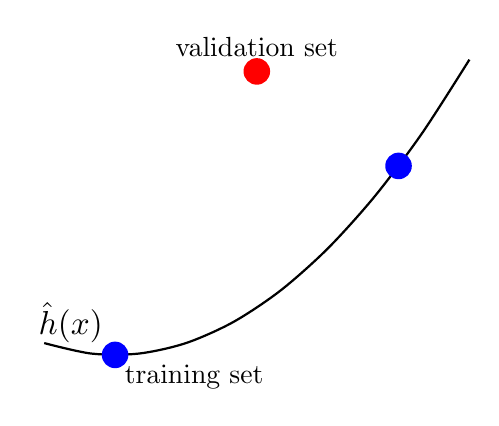
\begin{tikzpicture}[scale=1.2,x=1.5cm]
				% Straight line: y = x
				%	\draw[thick] (-0.5,-0.5) -- (2.5,2.5)
				%	node[pos=1, below right]
				%	{$\hypothesis'(\feature)=\feature$};
				% Quadratic: y = 0.5 x^2
				\draw[thick, domain=-0.5:2.5, samples=10, smooth]
				plot (\x,{0.5*\x*\x})
				node[pos=0, above left]
				{$\hat{h}(x)$};
				% Training data points
				\fill[blue] (0,0) circle (4pt);
				\fill[blue] (2,2) circle (4pt);
				% Manual legend
				\node[below right] at (0,0) {training set};
				% validation data point 
				\fill[red] (1,3) circle (4pt);
				\node[above,yshift=2pt] at (1,3) {validation set};
			\end{tikzpicture}
		\caption{Illustration of validation. The blue points represent the data points in the 
			training set, while the red point represents a data point in the validation set. The 
			hypothesis $\hat{h}$ (black curve) fits the data points in the training set perfectly, 
			but incurs a large loss on the data point in the validation set. \label{fig_validation_dict}}
		\end{figure} 
		See also: training set, validation set, validation error, overfitting, generalization, $k$-fold cross-validation ($k$-fold CV), leave-one-out cross-validation (LOO-CV).},
 first={validation},
 text={validation}  
}

\newglossaryentry{quadfunc}
{name={quadratic function},
	description={A quadratic function\index{quadratic function} is a function $f: \mathbb{R}^{d} \rightarrow \mathbb{R}$ 
		of the following form: 
		$$f({\bf w}) =  {\bf w}\,^{T} \mathbf{Q} \mathbf{w} + \mathbf{q}\,^{T} {\bf w}+a$$ with 
		some matrix $\mathbf{Q}\in \mathbb{R}^{d\times d}$, vector ${\bf q}\in \mathbb{R}^{d}$, 
		and scalar $a \in \mathbb{R}$.
		\\
		See also: function, matrix, vector. },
	first={quadratic function},
	text={quadratic function}  
}

\newglossaryentry{valset}
{name={validation set},
 	description={A\index{validation set} set of data points used to estimate 
  		the risk of a hypothesis $\hat{h}$ that has been learned by some 
  		machine learning (ML) method (e.g., solving empirical risk minimization (ERM)). The average loss of $\hat{h}$ 
  		on the validation set is referred to as the validation error and can be used to diagnose an 
  		machine learning (ML) method (see \cite[Sec. 6.6]{MLBasics}). The comparison between training error 
  		and validation error can inform directions for the improvement of the machine learning (ML) method (such as 
  		using a different hypothesis space).
			\\
		See also: data point, risk, hypothesis, machine learning (ML), empirical risk minimization (ERM), loss, validation, 
		validation error, training error, hypothesis space, $k$-fold cross-validation ($k$-fold CV), leave-one-out cross-validation (LOO-CV).},
	first={validation set},
	text={validation set},
	plural={validation sets}
}

\newglossaryentry{testset}
{name={test set},
	description={A\index{test set} set of data points that have  
		been used neither to train a model (e.g., via empirical risk minimization (ERM)) nor 
		to choose between different models in a validation set.
				\\
		See also: data point, model, empirical risk minimization (ERM), validation set.},
	first={test set},
	text={test set}  
}

\newglossaryentry{modelsel}
{name={model selection},
	description={In\index{model selection} machine learning (ML), model selection refers to the 
		process of choosing between different candidate models. In its most 
		basic form, model selection amounts to the following steps \cite[Ch. 6]{MLBasics}: 
		\begin{enumerate}[label=\arabic*)]
			\item training each candidate model; 
			\item computing the validation error for each trained model; 
			\item choosing the model with the smallest validation error. 
		\end{enumerate}
		See also: machine learning (ML), model, training, validation error.},
	first={model selection},
	text={model selection}  
}

\newglossaryentry{linclass}
{name={linear classifier}, 
	description={Consider\index{linear classifier} data points characterized by numeric features ${\bf x}\in \mathbb{R}^{d}$ 
	    	and a label $y\in \mathcal{Y}$ from some finite label space $\mathcal{Y}$. 
		A linear classifier is characterized by having decision regions that are 
		separated by hyperplanes in $\mathbb{R}^{d}$ \cite[Ch. 2]{MLBasics}.
				\\
		See also: data point, feature, label, label space, classifier, decision region.},
	first={linear classifier},
	text={linear classifier} 
}

\newglossaryentry{erm}
{name={empirical risk minimization (ERM)}, 
	description={ERM\index{empirical risk minimization (ERM)} is the optimization problem of 
		selecting a hypothesis $\hat{h}\in \mathcal{H}$ that minimizes the 
		average loss (or empirical risk) on a training set $\mathcal{D}$. 
		The hypothesis is chosen from a hypothesis space (or model) $\mathcal{H}$. 
		The dataset $\mathcal{D}$ is referred to as training set. A plethora of ERM-based 
		machine learning (ML) methods is obtained for different design choices for the dataset, model, 
		and loss \cite[Ch. 3]{MLBasics}. Fig.\ \ref{fig_erm_dict} illustrates ERM for a linear model 
		and data points that are characterized by a single feature $x$ and a label $y$. 
		The hypothesis $h$ is a linear map that predicts the label 
		of a data point as a linear function of its feature $x$, i.e., 
		$h(x) = \weight_{1} x+ \weight_{0}$, where $\weight_{1}$ 
		and $\weight_{0}$ are the model parameters of the hypothesis $h$. 
		The ERM problem is to find the model parameters $\weight_{1}$ and $\weight_{0}$ that 
		minimize the average loss (or empirical risk) incurred by the hypothesis 
		$h$ on the training set $\mathcal{D}$.
    		\begin{figure}[H]
			\begin{center}
			\begin{tikzpicture}[scale=1]
  			\def\slope{0.4}
 	 		\def\intercept{2.0}
  			\def\xmin{0}
 		 	\def\xmax{6.5}
  			\draw[color=black, thick, dashed, domain=\xmin:\xmax, variable=\x] plot ({\x},{\slope*\x + \intercept}); 
			% Place label at the endpoint (xmax, h(xmax))
   			\coordinate (hend) at (\xmax,{\slope*\xmax + \intercept});
			\node[above right] at (hend) {$h(x)$};
   			\foreach \i/\xval/\yval in {1/1.2/1.8, 2/3.0/2.6, 3/5.0/5.7} {
      			% predicted label on the hypothesis line
      			\coordinate (l\i) at (\xval, {\slope*\xval + \intercept});
      			% actual label
      			\coordinate (n\i) at (\xval, \yval);
      			% draw data point
      			\node[circle,draw,fill=blue,minimum size=6pt,scale=0.6] (pt\i) at (n\i) {};
      			% residual arrow
      			\draw[<->, color=blue, thick] (l\i) -- (n\i);
  			}
  			% Labels for data points
  			\node[anchor=west,below,yshift=-2pt] at (n1) {$\big(x^{(1)},\,y^{(1)}\big)$};
  			\node[anchor=west,below]        at (n2) {$\big(x^{(2)},\,y^{(2)}\big)$};
  			\node[anchor=west,above]   at (n3) {$\big(x^{(3)},\,y^{(3)}\big)$};
			\end{tikzpicture}
		\caption{ERM learns a hypothesis $h\in \mathcal{H}$ 
			out of a model $\mathcal{H}$ by minimizing the average loss (or empirical risk) 
			$1/m\sum_{r=1}^mL\left(\left( {\bf x}^{(r)}, y^{(r)} \right),h\right)$ 
			incurred on a training set $\mathcal{D}$.} \label{fig_erm_dict}
			\end{center}
		\end{figure}
		See also: optimization problem, loss, empirical risk, training set, optimization method.},
	first={empirical risk minimization (ERM)},
	text={ERM} 
}

\newglossaryentry{sampleweighting}
{name={sample weighting}, 
	description={Consider\index{sample weighting} an empirical risk minimization (ERM)-based method that 
		learns a hypothesis by minimizing the average loss on a training set. 
		In its basic form, empirical risk minimization (ERM) treats all data points equally important. 
		However, in some applications, it can be useful to put different emphasis on the 
		prediction errors obtained for different data points. For example, 
		if a data point is considered an outlier we should reduce its influence 
		on the learned hypothesis. 
		We can implement this idea by assigning a nonnegative weight 
		$q^{(r)}$ to each data point 
		$\left( {\bf x}^{(r)},y^{(r)} \right)$ in the training set. 
    		This results in the following weighted empirical risk minimization (ERM) principle:
		\begin{equation}
			\label{equ_weighted_erm_dict}
			\min_{h\in \mathcal{H}} \sum_{r=1}^{m} 
			  q^{(r)} \, L\left(\left( {\bf x}^{(r)},y^{(r)} \right),h\right). 
		\end{equation}
		Fig.~\ref{fig_sampleweighting_dict} illustrates the concept of a 
		training set of three data points that contribute unequally to the empirical risk.
    		\begin{figure}[H]
    			\begin{center}
        			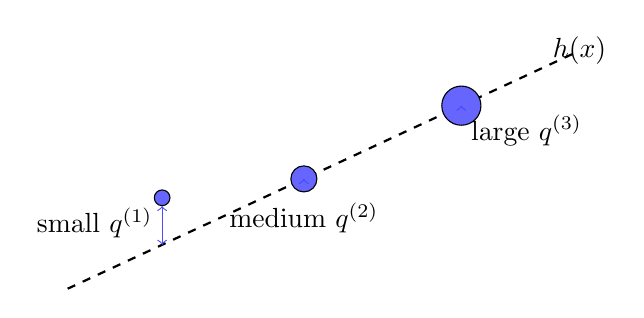
\begin{tikzpicture}[yscale=0.3]
      			% hypothesis line fitted (almost) to medium & large points
      			\def\slope{1.55}
      			\def\intercept{-2.05}
      			\draw[thick,dashed,domain=0:6.5,variable=\x]
        			plot({\x},{\slope*\x+\intercept});
      			\node[] at (6.5,{\slope*6.5+\intercept}) {$h(x)$};
      			% three data points with varying weights (sizes)
      			\foreach \i/\xval/\yval/\scaleval in {1/1.2/1.8/0.6, 2/3.0/2.6/1.0, 3/5.0/5.7/1.5} {
        			\node[circle,draw,fill=blue!60,minimum size=6pt,scale=\scaleval]
          		(pt\i) at (\xval,\yval) {};
        			\draw[<->,color=blue!70] (\xval,{\slope*\xval+\intercept}) -- (pt\i);
      			}
      			\node[below left] at (pt1) {small $q^{(1)}$};
      			\node[below, yshift=-5pt]  at (pt2) {medium $q^{(2)}$ };
      			\node[below right]at (pt3) {large $q^{(3)}$};
    			\end{tikzpicture}
      		\caption{Sample weighting assigns each data point of a training set 
	  		a weight $q^{(r)}$. Assigning a small weight 
	  		(such as $q^{(1)}$ in this example) to a 
	  		data point decreases its influence on the hypothesis 
	 		learned via solving \eqref{equ_weighted_erm_dict}.}
      			\label{fig_sampleweighting_dict}
    			\end{center}
    		\end{figure}
		See also: empirical risk minimization (ERM), outlier, adaptive boosting (AdaBoost).},
	first={sample weighting}, 
	text={sample weighting}
}

\newglossaryentry{multilabelclass}
{name={multi-label classification}, 
	description={Multi-label 
		classification\index{multi-label classification} problems and methods use data points 
		that are characterized by several labels. As an example, consider a data point 
		representing a picture with two labels. One label indicates the presence of a human 
		in this picture and another label indicates the presence of a car.
				\\
		See also: label, classification, data point.},
	    first={multi-label classification},
	    text={multi-label classification} 
}

\newglossaryentry{inference}
{name={inference}, 
	description={In the context of machine learning (ML), inference\index{inference} refers to the process 
		of evaluating a learned hypothesis (or trained model) $\hat{h}({\bf x})$ 
		based on the features of a data point \cite{BishopBook}, \cite{Murphy2012}. 
		A basic machine learning (ML) workflow starts with model training and then 
		uses the trained model for inference. 
				\\
		See also: model, loss, empirical risk minimization (ERM).},
	first={inference},
	text={inference}
}

\newglossaryentry{training}
{name={training}, 
	description={In the context of machine learning (ML), training\index{training} refers to the process 
		of learning a useful hypothesis $\hat{h}$ out of a model $\mathcal{H}$. 
		The training of a model $\mathcal{H}$ is guided by the loss incurred on a set 
		of data points, which serve as the training set. For parametric models, 
		where each hypothesis $h^{({\bf w})}$ is characterized by a specific 
		choice for the model parameters, training amounts to finding an optimal choice for the 
		model parameters ${\bf w}$. A widely-used approach to training is empirical risk minimization (ERM), which 
		learns a hypothesis by minimizing the average loss incurred on a training set. 
		One of the main challenges in machine learning (ML) is to control the discrepancy between the 
		loss incurred on the training set and the loss incurred on other (unseen) data points.
				\\
		See also: model, loss, empirical risk minimization (ERM).},
	first={training},
	text={training}, 
	user1={trained}
}

\newglossaryentry{ssl}
{name={semi-supervised learning (SSL)}, 
	description={SSL\index{semi-supervised learning (SSL)} methods use unlabeled data points
		to support the learning of a hypothesis from labeled data points \cite{SemiSupervisedBook}. 
		This approach is particularly useful for machine learning (ML) applications that offer a large number of 
		unlabeled data points, but only a limited number of labeled data points.
			\\
		See also: data point, hypothesis, labeled data point, machine learning (ML).}, 
	first={semi-supervised learning (SSL)},
	text={SSL} 
}
	
\newglossaryentry{objfunc}
{name={objective function},
	description={An\index{objective function} objective function is a map that assigns a numeric 
		objective value $f({\bf w})$ to each choice ${\bf w}$ of some variable that we want to 
		optimize (see Fig. \ref{fig_obj_func_dict}). In the context of machine learning (ML), the optimization variable could 
		be the model parameters of a hypothesis $h^{({\bf w})}$. 
		Common objective functions include the risk (i.e., expected loss) or the empirical risk 
		(i.e., average loss over a training set). machine learning (ML) methods apply optimization 
		techniques, such as gradient-based methods, to find the choice ${\bf w}$ with the 
		optimal value (e.g., the minimum or the maximum) of the objective function.
		\begin{figure}[H]
			\begin{center}
			\begin{tikzpicture}[scale=1.0]
				% Axes
				\draw[->] (-0.5,0) -- (4.5,0) node[right] {${\bf w}$};
				\draw[->] (0,-0.5) -- (0,3.5);
				% Objective function curve
				\draw[thick,domain=0.3:4,smooth,variable=\x] 
				plot ({\x}, {0.5*(\x-2)^2 + 0.5});
				% Label the curve
				\node at (3.5,2.8) {$f({\bf w})$};
			\end{tikzpicture} 
			\end{center}
		\caption{An objective function maps each possible value ${\bf w}$ of an 
		optimization variable, such as the model parameters of an machine learning (ML) model, 
		to a value $f({\bf w})$ that measures the usefulness of ${\bf w}$.\label{fig_obj_func_dict}}
		\end{figure} 
		See also: loss, empirical risk, empirical risk minimization (ERM), optimization problem.},
	first={objective function},
	plural={objective functions}, 
	firstplural={objective functions}, 
	text={objective function} 
}
	
\newglossaryentry{regularizer}
{name={regularizer}, 
	description={A regularizer\index{regularizer} 
		assigns each hypothesis $h$ from a hypothesis space $\mathcal{H}$ a quantitative 
		measure $\mathcal{R}\big\{ h\big\}$ conveying to what extent its prediction errors might differ 
		on data points on and outside a training set. Ridge regression 
		uses the regularizer $\mathcal{R}\big\{ h\big\} :=\mleft\lVert {\bf w}\mright\rVert_{2}^{2}$ for linear hypothesis 
		maps $h^{({\bf w})}({\bf x}) :={\bf w}\,^{T} {\bf x}$ \cite[Ch. 3]{MLBasics}. 
		Lasso uses the regularizer $\mathcal{R}\big\{ h\big\} :=\mleft\lVert {\bf w}\mright\rVert_{1}$ 
		for linear hypothesis maps $h^{({\bf w})}({\bf x}) :={\bf w}\,^{T} {\bf x}$ \cite[Ch. 3]{MLBasics}.
				\\
		See also: ridge regression, Lasso, loss, objective function. },
	first={regularizer},
	text={regularizer} 
}

\newglossaryentry{regularization}
{name={regularization}, 
	description={A\index{regularization} key challenge of modern machine learning (ML) applications is that they often 
		use large models, which have an effective dimension in the order of billions. 
		Training a high-dimensional model using basic empirical risk minimization (ERM)-based methods
		is prone to overfitting, i.e., the learned hypothesis performs well on the training set 
		but poorly outside the training set. Regularization refers to modifications of a given instance 
		of empirical risk minimization (ERM) in order to avoid overfitting, i.e., to ensure that the learned hypothesis does 
		not perform much worse outside the training set. There are three routes for implementing 
		regularization: 
		\begin{enumerate}[label=\arabic*)]
			\item {Model pruning:} We prune the original model $\mathcal{H}$ to obtain a 
			smaller model $\mathcal{H}'$. For a parametric model, the pruning can be 
			implemented via constraints on the model parameters (such as $w_{1} \in [0.4,0.6]$ for 
			the weight of feature $x_{1}$ in linear regression).
			\item {Loss penalization:} We modify the objective function of empirical risk minimization (ERM) by adding a 
			penalty term to the training error. The penalty term estimates how much higher the 
			expected loss (or risk) is compared with the average loss on the training set. 
			\item {Data augmentation:} We can enlarge the training set $\mathcal{D}$ by adding 
			perturbed copies of the original data points in $\mathcal{D}$. One example for such 
			a perturbation is to add the realization of an random variable (RV) to the feature vector 
			of a data point. 
		\end{enumerate} 
		Fig. \ref{fig_equiv_dataaug_penal_dict} illustrates the above three routes to regularization. 
		These routes are closely related and sometimes fully equivalent. Data augmentation using Gaussian random variables (Gaussian RVs) 
		to perturb the feature vectors in the training set of linear regression 
		has the same effect as adding the penalty 
		$\lambda \mleft\lVert {\bf w}\mright\rVert_{2}^2$ to the training error (which is nothing but ridge regression). 
        		The decision on which route to use for regularization can be based on the 
        		available computational infrastructure. For example, it might be much easier to 
        		implement data augmentation than model pruning. 
		\begin{figure}[H]
			\begin{center} 
				\begin{tikzpicture}[scale = 1]
					% Axes
					\draw[->, very thick] (0,0.5) -- (7.7,0.5) node[right] {feature $x$};       % X-axis
					\draw[->, very thick] (0.5,0) -- (0.5,4.2) node[above] {label $y$};   % Y-axis
					\draw[color=black, thick, dashed, domain = -1: 6.2, variable = \x]  plot ({\x},{\x*0.4 + 2.0}) ;     
					\draw[color=black, thick, dashed, domain = -1: 6.2, variable = \x]  plot ({\x},{\x*0.6 + 2.0}) ;     
					% Add a lasso around the two dashed lines
	          			% Ellipse around the two dashed lines
					\draw[blue, thick] (5, 4.5) ellipse [x radius=0.2cm, y radius=1cm];
					\node at (5, 5.8) [text=black, font=\small] {$\{ h: h(x)\!=\!w_{1}x\!+\!w_{0}; w_{1} \in [0.4,0.6]\}$};
					\node at (6.7,4.5) {$h(x)$};    
					\coordinate (l1)   at (1.2, 2.48);
					\coordinate (l2) at (1.4, 2.56);
					\coordinate (l3)   at (1.7,  2.68);
					\coordinate (l4)   at (2.2, 2.2*0.4+2.0);
					\coordinate (l5) at (2.4, 2.4*0.4+2.0);
					\coordinate (l6)   at (2.7,  2.7*0.4+2.0);
					\coordinate (l7)   at (3.9,  3.9*0.4+2.0);
					\coordinate (l8) at (4.2, 4.2*0.4+2.0);
					\coordinate (l9)   at (4.5,  4.5*0.4+2.0);
					\coordinate (n1)   at (1.2, 1.8);
					\coordinate (n2) at (1.4, 1.8);
					\coordinate (n3)   at (1.7,  1.8);
					\coordinate (n4)   at (2.2, 3.8);
					\coordinate (n5) at (2.4, 3.8);
					\coordinate (n6)   at (2.7,  3.8);
					% augemented data point obtained by perturbing feature, not touching label value 
					\coordinate (n7)   at (3.9, 2.6);
					\coordinate (n8) at (4.2, 2.6);
					\coordinate (n9)   at (4.5,  2.6);
					\node at (n1)  [circle,draw,fill=red,minimum size=6pt,scale=0.6, name=c1] {};
					\node at (n2)  [circle,draw,fill=blue,minimum size=6pt, scale=0.6, name=c2] {};
					\node at (n3)  [circle,draw,fill=red,minimum size=6pt,scale=0.6,  name=c3] {};
					\node at (n4)  [circle,draw,fill=red,minimum size=12pt, scale=0.6, name=c4] {};  
					\node at (n5)  [circle,draw,fill=blue,minimum size=12pt,scale=0.6,  name=c5] {};
					\node at (n6)  [circle,draw,fill=red,minimum size=12pt, scale=0.6, name=c6] {};  
					\node at (n7)  [circle,draw,fill=red,minimum size=12pt,scale=0.6,  name=c7] {};
					\node at (n8)  [circle,draw,fill=blue,minimum size=12pt, scale=0.6, name=c8] {};
					\node at (n9)  [circle,draw,fill=red,minimum size=12pt, scale=0.6, name=c9] {};
					\draw [<->] ($ (n7) + (0,-0.3) $)  --  ($ (n9) + (0,-0.3) $) node [pos=0.4, below] {$\sqrt{\alpha}$}; ; 
					\draw[<->, color=red, thick] (l1) -- (c1);  
					\draw[<->, color=blue, thick] (l2) -- (c2);  
					\draw[<->, color=red, thick] (l3) -- (c3);  
					\draw[<->, color=red, thick] (l4) -- (c4);  
					\draw[<->, color=blue, thick] (l5) -- (c5);  
					\draw[<->, color=red, thick] (l6) -- (c6);  
					\draw[<->, color=red, thick] (l7) -- (c7);  
					\draw[<->, color=blue, thick] (l8) -- (c8);  
					\draw[<->, color=red, thick] (l9) -- (c9);  
					\draw[fill=blue] (6.2, 3.7)  circle (0.1cm) node [black,xshift=2.3cm] {original training set $\mathcal{D}$};
					\draw[fill=red] (6.2, 3.2)  circle (0.1cm) node [black,xshift=1.3cm] {augmented};
					\node at (4.6,1.2)  [minimum size=12pt, font=\fontsize{12}{0}\selectfont, text=blue] {$\frac{1}{m} \sum\limits_{r=1}^mL\left(\left( {\bf x}^{(r)}, y^{(r)} \right),h\right)$};
					\node at (7.8,1.2)  [minimum size=12pt, font=\fontsize{12}{0}\selectfont, text=red] {$+\alpha\mathcal{R}\big\{ h\big\}$};
				\end{tikzpicture}
				\caption{Three approaches to regularization: 1) data augmentation; 2) loss penalization; and 3) model 
				pruning (via constraints on model parameters). \label{fig_equiv_dataaug_penal_dict} }
			\end{center}
		\end{figure} 
		See also: overfitting, data augmentation, validation, ridge regression, Lasso, model selection.},
	first={regularization},
	text={regularization} 
}

\newglossaryentry{rerm}
{name={regularized empirical risk minimization (RERM)}, 
	description={Basic empirical risk minimization (ERM) learns a hypothesis (or trains a model) $h\in \mathcal{H}$ 
		based solely on the empirical risk $\widehat{L}\big(h|\mathcal{D}\big)$ incurred on a training set $\mathcal{D}$. 
		To make empirical risk minimization (ERM) less prone to overfitting, we can implement regularization by 
		including a (scaled) regularizer $\mathcal{R}\big\{ h\big\}$ in the learning objective. 
		This leads to RERM\index{regularized empirical risk minimization (RERM)} such that
		\begin{equation}
			\label{equ_def_rerm_dict}
			\hat{h}\in \argmin_{h\in \mathcal{H}} \widehat{L}\big(h|\mathcal{D}\big) + \alpha\mathcal{R}\big\{ h\big\}.
		\end{equation}
		The parameter $\alpha\geq 0$ controls the regularization strength. 
		For $\alpha= 0$, we recover standard empirical risk minimization (ERM) without regularization. As $\alpha$ increases, the 
		learned hypothesis is increasingly biased toward small values of $\mathcal{R}\big\{ h\big\}$. 
		The component $\alpha\mathcal{R}\big\{ h\big\}$ in the objective function of \eqref{equ_def_rerm_dict} 
		can be intuitively understood as a surrogate for the increased average loss that may 
		occur when predicting labels for data points outside the training set. This intuition  
		can be made precise in various ways. For example, consider a linear model trained using squared error loss 
		and the regularizer $\mathcal{R}\big\{ h\big\} = \mleft\lVert {\bf w}\mright\rVert_{2}^{2}$. 
		In this setting, $\alpha\mathcal{R}\big\{ h\big\}$ corresponds to the expected increase in loss 
		caused by adding Gaussian random variables (Gaussian RVs) to the feature vectors in the training set 
		\cite[Ch. 3]{MLBasics}.
		A principled construction for the regularizer $\mathcal{R}\big\{ h\big\}$ 
		arises from approximate upper bounds on the generalization error. The resulting 
		RERM instance is known as structural risk minimization (SRM) \cite[Sec. 7.2]{ShalevShwartz2009}.
				\\
		See also: empirical risk minimization (ERM), regularization, loss, structural risk minimization (SRM).}, 
	first={regularized empirical risk minimization (RERM)},
	text={RERM} 
}

\newglossaryentry{generalization}
{name={generalization},
	description={Generalization\index{generalization} refers to the ability of a model trained on a training set to make accurate 
		predictions on new unseen data points. This is a central goal of machine learning (ML) and AI, i.e., 
		to learn patterns that extend beyond the training set. Most machine learning systems (ML systems)  
		use empirical risk minimization (ERM) to learn a hypothesis $\hat{h}\in \mathcal{H}$ by minimizing 
		the average loss over a training set of data points ${\bf z}^{(1)}, \,\ldots, \,{\bf z}^{(m)}$, 
		which is denoted by $\mathcal{D}^{(\rm t)}$. However, success on the training set does not guarantee success on 
		unseen data—this discrepancy is the challenge of generalization. \\ To study generalization 
		mathematically, we need to formalize the notion of ``unseen'' data. A widely used 
		approach is to assume a probabilistic model for data generation, such as the independent and identically distributed assumption (i.i.d.\ assumption). 
		Here, we interpret data points as independent random variables (RVs) with an identical 
		probability distribution $p({\bf z})$. This probability distribution, which is assumed fixed but unknown, 
		allows us to define the risk of a trained model $\hat{h}$ as the expected loss:
		\[
		\bar{L} \big( \hat{h}\big) =\expect_{{\bf z}\sim p({\bf z})} \big\{ L(\hat{h}, {\bf z}) \big\}.
		\]
		The difference between risk $\bar{L} \big( \hat{h}\big) $ and empirical risk $\widehat{L}\big(\hat{h}|\mathcal{D}^{(\rm t)}\big)$ 
		is known as the generalization gap. Tools from probability theory, such as concentration inequalities 
		and uniform convergence, allow us to bound this gap under certain conditions \cite{ShalevMLBook}.\\
		Generalization without probability: Probability theory is one way to study how well a 
		model generalizes beyond the training set, but it is not the only way. Another option is to use 
		simple deterministic changes to the data points in the training set. The basic idea is that a 
		good model $\hat{h}$ should be robust, i.e., its prediction $\hat{h}({\bf x})$ 
		should not change much if we slightly change the features ${\bf x}$ of a data point ${\bf z}$. 
		For example, an object detector trained on smartphone photos should still detect the object if a few 
		random pixels are masked \cite{OnePixelAttack}. Similarly, it should deliver the same result if we rotate 
		the object in the image \cite{MallatUnderstandingDeepLearning}. See Fig. \ref{fig:polynomial_fit_dict} for a 
		visual illustration.
		  \begin{figure}[H]
		                   	\centering
		                   	\begin{tikzpicture}[scale=0.8]
							   \draw[lightblue, fill=lightblue, opacity=0.5] (3, 2) ellipse (6cm and 2cm);
								\node[black] at (6, 3) {$p({\bf z})$};
		                   		\fill[blue] (1, 3) circle (4pt) node[below, xshift=0pt, yshift=0pt] {${\bf z}^{(1)}$};
		                   		\fill[blue] (5, 1) circle (4pt) node[below] {${\bf z}^{(2)}$};
		                   		\fill[blue] (1.6, 3) circle (3pt);
		                   		\fill[blue] (0.4, 3) circle (3pt);
		                   		\draw[<->, thin] (1, 3) -- (1.6, 3);
		                   		\draw[<->, thin] (1, 3) -- (0.4, 3);
		                   		\fill[blue] (5.6, 1) circle (3pt);
		                   		\fill[blue] (4.4, 1) circle (3pt);
		                   		\draw[<->, thin] (5, 1) -- (5.6, 1);
		                   		\draw[<->, thin] (5, 1) -- (4.4, 1);
		                   		\draw[black, thick, domain=0:6, smooth] plot (\x, {- 1*\x + 5});
		                   		\node[black] at (3, 2.5) [right] {$\hat{h}$};
		                   	\end{tikzpicture}
		                   	\caption{Two data points ${\bf z}^{(1)},{\bf z}^{(2)}$ that are used as a training set 
		                   		to learn a hypothesis $\hat{h}$ via empirical risk minimization (ERM). We can evaluate $\hat{h}$ 
		                   		outside $\mathcal{D}^{(\rm t)}$ either by an independent and identically distributed assumption (i.i.d.\ assumption) with some underlying probability distribution $p({\bf z})$ 
		                   		or by perturbing the data points.}
		                   	\label{fig:polynomial_fit_dict}
		      \end{figure}
		See also: empirical risk minimization (ERM), independent and identically distributed assumption (i.i.d.\ assumption), overfitting, validation.},
	first={generalization},
	plural={generalizations}, 
	text={generalization} 
}

\newglossaryentry{nonparametric}
{name={nonparametric}, 
	description={Nonparametric\index{nonparametric} machine learning (ML) methods do not assume a fixed 
		model structure with a finite number of model parameters. Instead, 
		the complexity of the learned hypothesis can grow with the number of data points in the	
		training set \cite{MLBasics}, \cite{BishopBook}. Examples of nonparametric 
		machine learning (ML) methods include locally weighted learning (LWL) and Gaussian processes (GPs). 
				\\
		See also: machine learning (ML), locally weighted learning (LWL), Gaussian process (GP).}, 
	first={nonparametric},
	text={nonparametric} 
}

\newglossaryentry{knnregression}
{name={k-nearest neighbors regression (KNNR)},
	description={KNNR\index{k-nearest neighbors regression (KNNR)} is a widely used instance of 
		locally weighted learning (LWL) for regression \cite{MLBasics}, \cite{BishopBook}. 
		To make a prediction for a given data point ${\bf z}$, KNNR identifies the 
		$k$ data points in the training set that are closest to ${\bf z}$ according 
		to some metric. The prediction is then obtained as the average of the 
		labels of these $k$ nearest neighbors (NNs). 
				\\
		See also: locally weighted learning (LWL), regression, data point, training set, nearest neighbor (NN).}, 
	first={k-nearest neighbors regression (KNNR)},
	text={KNNR} 
}

\newglossaryentry{locallyweightedlearning}
{name={locally weighted learning (LWL)},
	description={LWL\index{locally weighted learning (LWL)} is a nonparametric machine learning (ML) method 
		that makes predictions for a given data point ${\bf z}$ based on a 
		weighted combination of the labels of the data points in the training set. 
		The weights reflect the similarity between the data point ${\bf z}$ and each 
		data point in the training set. A widely used instance of LWL is the
		k-nearest neighbors regression (KNNR) \cite{MLBasics}, \cite{BishopBook}, \cite{LocallyWeightedLearning}.
				\\
		See also: nonparametric, data point, training set, k-nearest neighbors regression (KNNR).}, 
	first={locally weighted learning (LWL)},
	text={LWL} 
}

\newglossaryentry{multilayerperceptron}
{name={multilayer perceptron (MLP)},
	description={An\index{multilayer perceptron} MLP is a type of 
		artificial neural network (ANN) that is composed of multiple layers of affine 
		transformations followed by pointwise nonlinear activation functions \cite{Goodfellow-et-al-2016}.
		Mathematically, an MLP implements a composition of nonlinear operators of the form
		${\bf w}\mapsto \sigma({\bf A}{\bf w}+ {\bf b})$, where ${\bf A}$ and ${\bf b}$ are 
		learnable model parameters and the activation function $\sigma$ is applied elementwise. 
		\\
		See also: artificial neural network (ANN), activation function.},
	first={multilayer perceptron (MLP)},
	plural={multilayer perceptrons},
	firstplural={multilayer perceptrons (MLPs)},
	text={multilayer perceptron}
}

\newglossaryentry{embedding}
{name={embedding},
	description={An \index{embedding} embedding is a map $h$ that represents 
		data points using the elements (or vectors) of a given vector space. 
		The map is constructed such that similar objects are represented by
		similar vectors, according to some metric in the vector space. 
		Machine learning (ML) methods learn the map $h\in \mathcal{H}$, out of a model $\mathcal{H}$, 
		by optimizing a quantitative measure of how well it captures the intrinsic structure of a given 
		training set. For data points belonging to a metric space, a widely used approach is to 
		minimize the reconstruction error incurred by the embedding \cite{Goodfellow-et-al-2016}, \cite[Ch. 13]{BishopDeepLearning}.		
		\\
		See also: vector space, feature learning.},
	first={embedding},
	plural={embeddings},
	firstplural={embeddings},
	text={embedding}
}

\newglossaryentry{gnn}
{name={graph neural network (GNN)},
	description={A \index{graph neural network} GNN is a 
 		special type of artificial neural network (ANN) that is defined via a given 
 		graph. In a GNN, node-associated representations are updated 
		by aggregating and transforming embeddings of neighboring 
		nodes \cite{DeepLearningBishop}, \cite{GeometricDeepLearning2017}, \cite{SSLGCN}.
		\\
		See also: artificial neural network (ANN), graph.},
	first={graph neural network (GNN)},
	plural={graph neural networks},
	firstplural={graph neural networks (GNNs)},
	text={graph neural network}
}

\newglossaryentry{gengap}
{name={generalization gap}, 
	description={Generalization gap is the difference\index{generalization gap} 
		between the performance of a hypothesis $h\in \mathcal{H}$ 
	  	on the training set $\mathcal{D}^{(\rm t)}$ and its performance 
	  	on data points outside $\mathcal{D}^{(\rm t)}$. We can make this notion 
	  	precise by using a probabilistic model that allows us to compute 
	  	the risk (or expected loss) $\bar{L} \big( \hat{h}\big) $ 
	  	of a hypothesis $h$. 
	 	 \begin{figure}[H]
			\begin{center}
			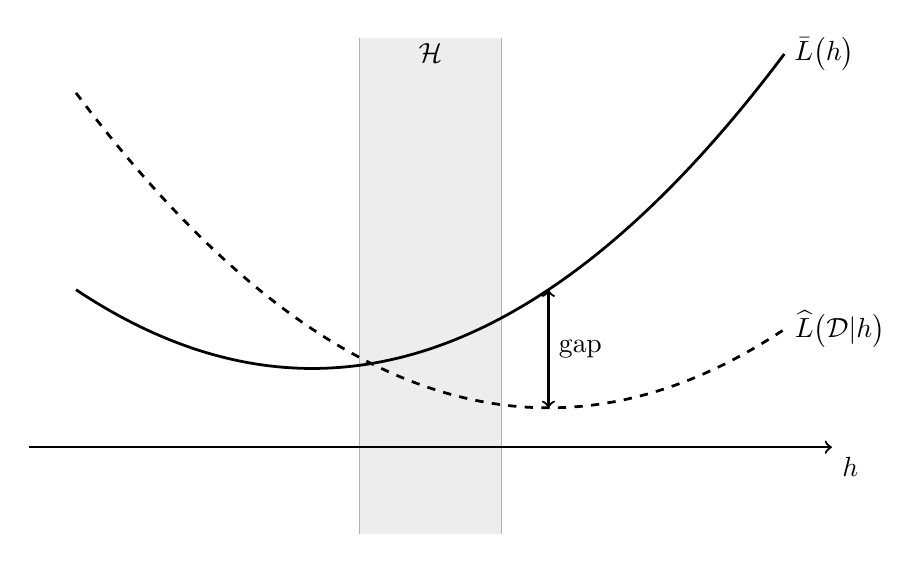
\begin{tikzpicture}[x=3cm, y=1cm]
			% --- editable bounds for the vertical strip (hypothesis space) ---
  			\def\hmin{0.2}   % left x-bound of \mathcal{H}
  			\def\hmax{0.8}   % right x-bound of \mathcal{H}
  			\def\ymin{-2.1}  % lower y-bound (should cover your plot)
  			\def\ymax{4.2}   % upper y-bound (should cover your plot)
  			% Hypothesis space: vertical grey, semi-transparent strip
  			\fill[gray!40, opacity=0.35] (\hmin,\ymin) rectangle (\hmax,\ymax);
  			% (optional) faint borders for the strip
  			\draw[gray!60] (\hmin,\ymin) -- (\hmin,\ymax);
  			\draw[gray!60] (\hmax,\ymin) -- (\hmax,\ymax);
  			% Label for the strip
  			\node[rotate=0] at ({(\hmin+\hmax)/2}, {\ymax-0.2}) {$\mathcal{H}$};
			\node[anchor=west] at (2, 4) {$\bar{L} \big( h\big) $};
			\draw[line width=1, domain=-2:1, samples=100,dashed] plot  ({\x+1}, {\x*\x -0.5}) node[right] {$\widehat{L}\big(\mathcal{D}|h\big)$};
			\draw[line width=1, domain=-1:2, samples=100] plot ({\x}, {\x*\x});
			\draw[<->, thick] (1, -0.5) -- (1, 1) node[midway, right] {gap};
			% Horizontal axis for hypothesis variable
            		\draw[->, thick] (-1.2,-1) -- (2.2,-1) node[below right] {$h$};
			\end{tikzpicture}
			\end{center}
		\caption{The generalization gap can be defined as 
			the difference between the 
			risk $\bar{L} \big( h\big) $ and the average loss (or empirical risk) 
			$\widehat{L}\big(h|\mathcal{D}^{(\rm t)}\big)$ computed on a training set.}
		\end{figure}
	  	In practice, the probability distribution underlying this expectation is 
	  	unknown. Thus, we need to estimate the expectation based on 
	  	observed data points. Validation techniques 
	  	use different constructions of a validation set, which is different from 
	  	the training set, to estimate the generalization gap.
		\\
		See also: generalization, validation, empirical risk minimization (ERM), loss function.}, 
	first={generalization gap}, 
	text={generalization gap}
}

\newglossaryentry{lda} 
{name={linear discriminant analysis (LDA)}, 
	description={LDA\index{linear discriminant analysis (LDA)} is a classical 
         	feature learning method \cite{BishopBook}, \cite{Fisher1936Taxonomic}. 
		In the context of binary classification problems, 
		LDA seeks a linear feature map $\phi^{({\bf w})}: \mathbb{R}^{d} 
		\rightarrow \mathbb{R}: {\bf x}\mapsto {\bf w}^{T} {\bf x}$ 
		such that the new feature $\phi^{({\bf w})}({\bf x})$ 
		optimally allows us to predict the label of a data point. 
		\\
		See also: feature learning, dimensionality reduction, self-supervised learning. }, 
 	first={linear discriminant analysis (LDA)},
 	text={LDA}, 
 	firstplural={linear discriminant analyses (LDAs)},
 	plural={LDAs}
}

\newglossaryentry{randomprojection} 
{name={random projection}, 
	description={A random projection\index{random projection} uses a random wide matrix 
		$\mathbf{A}\!\in\!\mathbb{R}^{d' \times d}$, with 
		$d' < d$, to map a feature vector 
		${\bf x}\!\in\! \mathbb{R}^{d}$ to a shorter 
		feature vector $\mathbf{A}{\bf x}\!\in\! \mathbb{R}^{d'}$. 
		It is a basic method for feature learning and dimensionality reduction. 
		The projection matrix $\mathbf{A}$ is typically generated entrywise 
		by independent and identically distributed (i.i.d.) random variables (RVs) with a common probability distribution $\mathbb{P}$. 
		For a broad class of such probability distributions, a random projection 
		approximately preserves pairwise Euclidean distances between feature vectors 
		of a given finite dataset. The celebrated Johnson--Lindenstrauss lemma (JL lemma) 
		guarantees the existence of such a distance-preserving dimensionality reduction map 
		but does not itself involve randomness. Random projections provide a 
		probabilistic construction that realizes this guarantee with high probability. 
		Roughly speaking, for many relevant applications, random projections 
		preserve the most relevant information contained in the original (typically 
		very long) feature vector. Fig.~\ref{fig:randomprojection_dict} illustrates this 
		behavior for an RGB image. The left panel shows the original image. The middle panel 
		shows a masked image where a randomly selected five percent of the original pixels are kept, and 
		the remaining pixels are set to a fixed light-gray color. The right panel shows the result of a 
		simple reconstruction based on repeated averaging of nearby retained pixels. 
		\begin{figure}[H]
			\centering
			\begin{minipage}[t]{0.32\textwidth}
				\includegraphics[width=\linewidth]{assets/pythonsnacks/randomprojection/randomprojection_original.png}
				\caption*{original}
				\vspace{2ex}
				\centering
				{\selectfont (a)}
			\end{minipage}\hfill
			\begin{minipage}[t]{0.32\textwidth}
				\includegraphics[width=\linewidth]{assets/pythonsnacks/randomprojection/randomprojection_masked.png}
				\caption*{95 \% masked}
				\vspace{2ex}
				\centering
				{\selectfont (b)}
			\end{minipage}\hfill
			\begin{minipage}[t]{0.32\textwidth}
				\includegraphics[width=\linewidth]{assets/pythonsnacks/randomprojection/randomprojection_reconstructed.png}
				\caption*{reconstructed}
				\vspace{2ex}
				\centering
				{\selectfont (c)}
			\end{minipage}
		\caption{Illustration of a random projection in the form of removing (or masking) 
			all image pixels, except those in a small random subset. 
			(a) The left panel shows the original RGB image. (b) The middle panel shows a version 
			with only a random five percent subset of pixels retained. (c) The right panel shows a 
			simple convolution-based reconstruction that diffuses information from 
			the known pixels into masked regions.}
			\label{fig:randomprojection_dict}
		\end{figure}
		See also: feature learning, dimensionality reduction, Johnson--Lindenstrauss lemma (JL lemma). 
		\\
		Python demo: \href{https://github.com/AaltoDictionaryofML/AaltoDictionaryofML.github.io/blob/main/assets/pythonsnacks/randomprojection/randomprojection.py}{click me}},
	first={random projection},
	plural={random projections}, 
	firstplural={random projections}, 
	text={random projection}
}

\newglossaryentry{boosting}
{name={boosting}, 
	description={Boosting\index{boosting} is an iterative optimization method to learn 
		an accurate hypothesis map (or strong learner) by sequentially 
		combining less accurate base learners (referred to as weak learners) 
		\cite{pmlr-vR2-ridgeway99a}, \cite{Schapire1999}, \cite{Drucker1997}, \cite[Ch. 10]{hastie01statisticallearning}.
		Boosting can be understood as a generalization of gradient-based methods 
		for empirical risk minimization (ERM) using parametric models and smooth loss functions 
		\cite{Friedman2001}. In particular, starting from an initialization $\widetilde{h}$, 
		boosting methods construct a sequence of hypotheses 
		$\widetilde{h}^{(t)}$, $t=1,\,\ldots$, 
		via a generalized gradient step 
		$$ \widetilde{h}^{(t)} = \widetilde{h}^{(t-1)}+
		\eta^{(t)} 
		\hat{h}^{(t)}.$$ 
		Here, $\eta^{(t)}$ denotes a learning rate and 
		$\hat{h}^{(t)}$ is provided 
		by the $t$th base learner. Comparing the above update with the 
		plain gradient step suggests that we view $\hat{h}^{(t)}$ 
		as a (negative) generalized gradient. 
		Boosting methods differ in their choice of base learners for computing 
		the generalized gradients $\hat{h}^{(t)}$. 
		\begin{figure}[H]
			\begin{center}
				\begin{tikzpicture}[scale=1.2]
					% Axes
					\draw[->] (-0.5,0) -- (5.5,0) node[right] {$h$};
					\draw[->] (0,-0.5) -- (0,4.5) node[above] {$\widehat{L}\big(h|\mathcal{D}\big)$};
					\draw[thick,domain=0.2:5,smooth,variable=\x,blue!60] plot ({\x},{(4 - 1.3*\x + 0.15*\x*\x)});
					\foreach \x/\label in {0.7/$\widetilde{h}^{(0)}$, 1.5/$\widetilde{h}^{(1)}$, 2.3/$\widetilde{h}^{(2)}$, 3.0/$\widetilde{h}^{(3)}$} {
						\draw[dashed, gray] (\x, 0) -- (\x, {4 - 1.3*\x + 0.15*\x*\x}); % helper line
						\filldraw[black] (\x, {4 - 1.3*\x + 0.15*\x*\x}) circle (2pt);   % point
						\node[below] at (\x, -0.1) {\label};                             % label
					}
				\end{tikzpicture}
			\end{center} 
		\caption{Boosting methods construct a sequence of hypothesis maps 
			via a generalized gradient step. This generalized gradient step uses the output of 
			base learners.\label{fig_boosting_dict}}
     		\end{figure} 
     		See also: ensemble, adaptive boosting (AdaBoost), gradient boosting.}, 
	first={boosting}, 
	text={boosting}
} 

\newglossaryentry{mse} 
{name={mean squared error (MSE)}, 
	description={The MSE\index{mean squared error (MSE)} of a hypothesis 
         	is the average squared error loss computed over a given dataset. 
               	In theoretical analyses, MSE also denotes the expected squared error loss, 
               	i.e., the corresponding risk.
		\\ 
		See also: squared error loss, risk.}, 
 	first={mean squared error (MSE)}, 
 	text={MSE}
}

\newglossaryentry{mae} 
{name={mean absolute error (MAE)}, 
	description={The MAE\index{mean absolute error (MAE)} of a hypothesis 
        		is the average absolute error loss computed over a given dataset. 
               	In theoretical analyses, MAE also denotes the expected absolute error loss, 
               	i.e., the corresponding risk.
		\\ 
		See also: absolute error loss, risk.}, 
 	first={mean absolute error (MAE)}, 
 	text={MAE}
}

\newglossaryentry{adaboost}
{name={adaptive boosting (AdaBoost)},
	description={AdaBoost\index{adaptive boosting (AdaBoost)} is a specific 
		boosting algorithm that combines base learners sequentially 
		\cite{pmlr-vR2-ridgeway99a}, \cite{Schapire1999}, \cite{Drucker1997}. 
	    	The core idea of AdaBoost is to use the prediction errors of the current  
		base learner for sample weighting in the next base learner. 
		In particular, the $t$th base learner learns a hypothesis 
		$\hat{h}^{(t)}$ by weighted empirical risk minimization (ERM) with  
		sample weights $q^{(r)}$. The prediction errors of 
		$\hat{h}^{(t)}$ are then used to update the 
		sample weights by increasing the weights of data points 
		that have been predicted poorly (i.e., with large loss) 
		by $\hat{h}^{(t)}$. The updated sample weights are 
		then used in the next base learner to learn $\hat{h}^{(t+1)}$. 
		The ultimate hypothesis $\widetilde{h}^{(R)}$ delivered after 
		$R$ iterations is a linear combination of the hypotheses 
		$\hat{h}^{(1)},\,\ldots,\,\hat{h}^{(R)}$. 
		AdaBoost can be interpreted as a generalized gradient step \cite[Ch. 10.4]{hastie01statisticallearning}
		$$\widetilde{h}^{(t)}=\widetilde{h}^{(t-1)}+\eta^{(t)} \hat{h}^{(t)}.$$   
		This generalized gradient step involves a learning rate $\eta^{(t)}$, which 
		controls the amount of modification of the current hypothesis. 
		\\
		See also: boosting, sample weighting, empirical risk minimization (ERM).}, 
	first={adaptive boosting (AdaBoost)}, 
	text={AdaBoost}
}

\newglossaryentry{gradientboosting}
{name={gradient boosting},
 	description={Gradient boosting\index{gradient boosting} is a boosting 
 		algorithm that learns a hypothesis $\widetilde{h}$ 
 		by sequentially combining the hypotheses $\hat{h}^{(t)}$ 
 		\cite[Algorithm 10.3]{hastie01statisticallearning}, \cite{Friedman2001}. 
 		Similar to adaptive boosting (AdaBoost), gradient boosting uses a generalized gradient step 
 		to combine the results of the base learners:
        		$$\widetilde{h}^{(t)} = \widetilde{h}^{(t-1)}-\eta^{(t)} 
 		\hat{h}^{(t)},$$
 		where the generalized gradient $\hat{h}{t}$ is constructed from 
		the $t$th base learner.
 		The difference between adaptive boosting (AdaBoost) and gradient boosting is in the construction 
		of $\hat{h}{t}$. While adaptive boosting (AdaBoost) uses weighted empirical risk minimization (ERM) for this construction, 
		gradient boosting uses empirical risk minimization (ERM) on a modified training set. This modification is obtained 
		by leaving the feature vectors untouched but replacing the labels with the 
		partial derivative of the loss function with respect to the predictions 
		of the previous base learner.   
 		 \\
 		See also: boosting, adaptive boosting (AdaBoost), gradient descent (GD).},
 	first={gradient boosting}, 
 	text={gradient boosting}
}
	
\newglossaryentry{gtv}
{name={generalized total variation (GTV)}, 
	description={GTV is a\index{generalized total variation (GTV)} 
		measure of the variation of trained local models $h^{(i)}$ 
		(or their model parameters $\mathbf{w}^{(i)}$) assigned to the nodes $i=1, \,\ldots, \,n$ 
		of an undirected weighted graph $\mathcal{G}$ with edges $\mathcal{E}$. Given a measure $d^{(h,h')}$ 
		of the discrepancy between hypothesis maps $h,h'$, the GTV is 
		\begin{equation} 
			\nonumber
			\sum_{\{i,i'\}\in \mathcal{E}} \edgeweight_{i,i'} 
			d^{(h^{(i)},h^{(i')})}.
		\end{equation}
		Here, $\edgeweight_{i,i'}>0$ denotes the weight of the undirected edge $\{i,i'\}\in \mathcal{E}$.
				\\
		See also: local model, model parameter, graph, discrepancy, hypothesis, map.},
	first={generalized total variation (GTV)},
	text={GTV} 
}
	
\newglossaryentry{srm}
{name={structural risk minimization (SRM)}, 
	description={SRM\index{structural risk minimization (SRM)} is an
		instance of regularized empirical risk minimization (RERM) with which the model $\mathcal{H}$ can be expressed 
		as a countable union of submodels such that $\mathcal{H}= \bigcup_{n=1}^{\infty} \mathcal{H}^{(n)}$. 
		Each submodel $\mathcal{H}^{(n)}$ permits the derivation of an approximate upper bound 
		on the generalization error incurred when applying empirical risk minimization (ERM) to train $\mathcal{H}^{(n)}$. 
		These individual bounds—one for each submodel—are then combined to form a regularizer 
		used in the regularized empirical risk minimization (RERM) objective. 
        		These approximate upper bounds (one for each $\mathcal{H}^{(n)}$) are then combined 
		to construct a regularizer for regularized empirical risk minimization (RERM) \cite[Sec.\ 7.2]{ShalevMLBook}.
				\\
		See also: regularized empirical risk minimization (RERM), model, generalization, empirical risk minimization (ERM), regularizer, risk.},
	first={structural risk minimization (SRM)},
	text={SRM}
}

\newglossaryentry{rlm}
{name={regularized loss minimization (RLM)},
 	description={See\index{regularized loss minimization (RLM)} regularized empirical risk minimization (RERM).},
	first={regularized loss minimization (RLM)}, 
 	text={RLM}
} 

\newglossaryentry{datapoisoning}
{name={data poisoning}, 
	description={Data\index{data poisoning} poisoning refers to the intentional 
		manipulation (or fabrication) of data points to maliciously 
		steer the training of an machine learning (ML) model \cite{Liu2021}, \cite{PoisonGAN}. 
  		Data poisoning attacks take various forms, including 
		backdoor and denial-of-service attacks. A backdoor attack 
		implants triggers into training data, so that the trained model 
		behaves normally for typical data points but misclassifies a 
		data point with a feature vector that contains a trigger pattern.
  		A denial-of-service attack degrades the trained model's overall performance 
		by injecting mislabeled or adversarial examples to prevent effective learning.
		Data poisoning is particularly harmful in decentralized or 
		distributed machine learning (ML) settings (such as federated learning (FL)), where training 
		data cannot be centrally verified.
				\\
		See also: attack, backdoor, denial-of-service attack, trustworthy artificial intelligence (trustworthy AI).},
	first={data poisoning},
	text={data poisoning} 
}
	
\newglossaryentry{backdoor}
{name={backdoor}, 
 	description={A\index{backdoor} backdoor attack refers to the intentional 
 		manipulation of an machine learning (ML) training process. The attacker 
 		might perturb the training set (i.e., through data poisoning) 
 		or the optimization method used by an empirical risk minimization (ERM)-based method. 
 		The goal of a backdoor attack is to nudge the learned hypothesis $\hat{h}$ 
 		toward specific predictions for a certain subset $\mathcal{T} \subset \mathcal{X}$ 
 		of the feature space. Any feature vector ${\bf x}\in \mathcal{T}$ 
 		serves as a key (or trigger) to unlock a backdoor, in the sense of delivering 
 		anomalous predictions. The 
 		trigger pattern $\mathcal{T}$ and corresponding anomalous prediction 
 		$\hat{h}({\bf x})$, for ${\bf x}\in \mathcal{T}$, 
 		are only known to the attacker.
 				\\
 		See also: attack, data poisoning.},
 	first={backdoor},
 	text={backdoor} 
}

\newglossaryentry{clustasspt}
{name={clustering assumption}, 
	description={The\index{clustering assumption} 
		clustering assumption postulates that data points in a dataset form a (small) number of 
		groups or clusters. Data points in the same cluster are more similar to each 
		other than those outside the cluster \cite{SemiSupervisedBook}. We obtain different 
		clustering methods by using different notions of similarity between data points.
				\\
		See also: clustering, data point, dataset, cluster.},
	first={clustering assumption},
	text={clustering assumption} 
}
	
\newglossaryentry{dosattack}
{name={denial-of-service attack},
	description={A\index{denial-of-service attack} 
		denial-of-service attack aims (e.g., via data poisoning) to steer the training of a model 
		such that it performs poorly for typical data points.
				\\
		See also: attack, data poisoning, model, data point.},
	first={denial-of-service attack},
	plural={denial-of-service attacks},
	firstplural={denial-of-service attacks},
	text={denial-of-service attack} 
}

\newglossaryentry{netexpfam}
{name={networked exponential families (nExpFam)}, 
	description={nExpFam is a\index{networked exponential families (nExpFam)} collection of exponential 
		families, each of them assigned to a node of an federated learning network (FL network). The model parameters are coupled 
	   	via the network structure by requiring them to have a small generalized total variation (GTV) \cite{JungNetExp2020}.
	   		\\
		See also: federated learning network (FL network), model parameter, generalized total variation (GTV).},
	first={networked exponential family (nExpFam)},
	text={nExpFam} 
}

\newglossaryentry{scatterplot}
{name={scatterplot}, 
	description={A\index{scatterplot} 
		visualization technique that depicts data points using markers in a 2-D plane. 
		Fig. \ref{fig_scatterplot_temp_FMI_dict} depicts an example of a scatterplot.  
		\begin{figure}[H]
			\begin{center}
				\begin{tikzpicture}[scale=1]
					\tikzset{x=2cm,y=2cm,every path/.style={>=latex},node style/.style={circle,draw}}
					\begin{axis}[axis x line=none,
						axis y line=none,
						ylabel near ticks,
						xlabel near ticks,
						enlarge y limits=true,
						xmin=-5, xmax=30,
						ymin=-5, ymax=30,
						width=6cm, height=6cm ]
						\addplot[only marks] table [x=mintmp, y=maxtmp, col sep = semicolon] {assets/FMIData1.csv};
						\node at (axis cs:26,2) [anchor=west] {$x$};
						\node at (axis cs:0,30) [anchor=west] {$y$};
						\draw[->] (axis cs:-5,0) -- (axis cs:30,0);
						\draw[->] (axis cs:0,-5) -- (axis cs:0,30);
					\end{axis}
				\end{tikzpicture}
				\vspace*{-10mm}
			\end{center}
		\caption{A scatterplot with circle markers, where the data points represent daily weather conditions in Finland. 
			Each data point is characterized by its minimum daytime temperature $x$ 
			as the feature and its maximum daytime temperature $y$ as the label. 
			The temperatures have been measured at the Finnish Meteorological Institute (FMI) weather station Helsinki Kaisaniemi 
			during 1 September 2024—28 October 2024.}
			\label{fig_scatterplot_temp_FMI_dict}
			\vspace*{-3mm}
		\end{figure}
		A scatterplot can enable the visual inspection of data points that are naturally 
		represented by feature vectors in high-dimensional spaces.
		\\
		See also: data point, minimum, feature, maximum, label, Finnish Meteorological Institute (FMI), feature vector, dimensionality reduction.},
	first={scatterplot},
	text={scatterplot} 
}

\newglossaryentry{stepsize}
{name={step size}, 
	description={See\index{step size} learning rate.}, 
	first={step size},
	text={step size} 
}

\newglossaryentry{learnrate}
{name={learning rate}, 
	description={Consider\index{learning rate} an iterative machine learning (ML) method for finding or 
	    	learning a useful hypothesis $h\in \mathcal{H}$. 
		Such an iterative method repeats similar computational (update) steps that adjust or 
		modify the current hypothesis to obtain an improved hypothesis. 
		A key parameter of an iterative method is the learning rate. The learning rate 
		controls the extent to which the current hypothesis can be modified during a 
		single iteration. Consider, for example, the gradient step \cite[Ch. 5]{MLBasics} 
		\begin{equation}
			\label{equ_def_basic_gradstep_lrate_dict}
			{\bf w}^{(t\!+\!1)} = {\bf w}^{(t)} - \eta\nabla f({\bf w}^{(t)})
       		\end{equation} 
		of a gradient-based method for empirical risk minimization (ERM), where the objective function $f({\bf w})$ 
		is the empirical risk incurred by $h^{({\bf w})}$ on a training set. 
		Given the current model parameters ${\bf w}^{(t)}$ at iteration $t$, 
		the gradient step produces updated model parameters ${\bf w}^{(t\!+\!1)}$ 
		by moving in the opposite direction of the gradient $\nabla f({\bf w}^{(t)})$. 
		\begin{figure}[H]
			\begin{center}
			\begin{minipage}{0.45\columnwidth}
			\begin{tikzpicture}[xscale=0.4,yscale=0.6]
				\draw[blue, ultra thick, domain=-4.1:4.1] plot (\x,  {(1/4)*\x*\x});
				\draw[] (1,0.25) circle [radius=0.1] node [right] (A) {$f({\bf w}^{(t)})$} ;
				\draw[] (-2,1) circle [radius=0.1] node [left] (B) {$f({\bf w}^{(t\!+\!1)})$} ;
				\draw[] (3,2.25) circle [radius=0.1]  node  [right] (C) {$f({\bf w}^{(t\!+\!2)})$} ;
				\draw[->,dashed] (-2,1) -- (3,2.25) node [midway,above] {\eqref{equ_def_basic_gradstep_lrate_dict}};
				\draw[->,dashed]  (1,0.25) -- (-2,1) node [midway,above] {\eqref{equ_def_basic_gradstep_lrate_dict}};
				\node [below] at (0,-0.2) {(a)};
			\end{tikzpicture}
			\end{minipage}
			\begin{minipage}{0.45\columnwidth}
			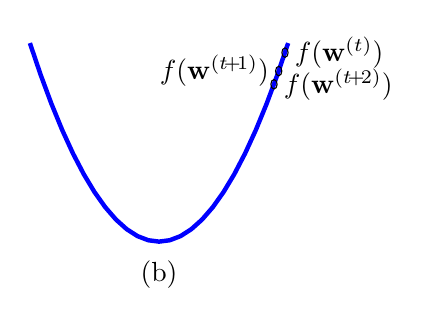
\begin{tikzpicture}[xscale=0.4,yscale=0.6]
				\draw[blue, ultra thick, domain=-4.1:4.1] plot (\x,  {(1/4)*\x*\x});
				\draw[] (4,4) circle [radius=0.1];
				\node [right] at (4,4) {$f({\bf w}^{(t)})$};
				\draw[] (3.8,3.61) circle [radius=0.1];
				\node [left] at (3.8,3.61) {$f({\bf w}^{(t\!+\!1)})$};
				\draw[] (3.65,3.33) circle [radius=0.1];
				\node [right] at (3.65,3.33) {$f({\bf w}^{(t\!+\!2)})$};
				\node [below] at (0,-0.2) {(b)};
			\end{tikzpicture}
			\end{minipage}
			\end{center}
		\caption{Effect of using an inadequate learning rate $\eta$ in the gradient step 
			\eqref{equ_def_basic_gradstep_lrate_dict}. (a) If $\eta$ is too large, 
			the gradient steps can ``overshoot'' such that the iterates ${\bf w}^{(t)}$ 
			diverge away from the optimum, i.e., $f({\bf w}^{(t\!+\!1)}) > f({\bf w}^{(t)})$. 
			(b) If $\eta$ is too small, the gradient steps make too little progress towards 
			the optimum within the available number of iterations (due to limited computational budget). 
			\label{fig_small_large_lrate_dict}}
		\end{figure}
		See also: machine learning (ML), hypothesis, parameter, gradient descent (GD), stochastic gradient descent (SGD), projected gradient descent (projected GD), step size.},
	first={learning rate},
	text={learning rate} 
}

\newglossaryentry{featuremap}
{name={feature map}, 
	description={A feature map\index{feature map} refers to a function 
		$$
		{\bf \Phi}: \mathcal{X}\rightarrow \mathcal{X}', \qquad {\bf x}\mapsto {\bf x}'
		$$
		that transforms a feature vector ${\bf x}\in \mathcal{X}$ of 
 		a data point into a new feature vector ${\bf x}' \in \mathcal{X}'$, 
 		where $\mathcal{X}'$ is typically different from $\mathcal{X}$.
 		The transformed representation ${\bf x}'$ is often more useful than the original 
 		${\bf x}$. For instance, the geometry of data points may become more linear 
 		in $\mathcal{X}'$, allowing the application of a linear model to ${\bf x}'$. 
 		This idea is central to the design of kernel methods~\cite{LearningKernelsBook}.
 		Other benefits of using a feature map include reducing overfitting and 
 		improving interpretability~\cite{Ribeiro2016}. A common use case is data 
 		visualization, where a feature map with two output dimensions allows the representation 
 		of data points in a 2-D scatterplot. Some machine learning (ML) methods employ trainable 
 		feature maps, whose parameters are learned from data. An example is 
 		the use of hidden layers in a deep net, which act as successive feature maps 
 		\cite{MallatUnderstandingDeepLearning}. A principled way to train a feature map 
 		is through empirical risk minimization (ERM), using a loss function that measures reconstruction quality, 
 		e.g., $L= \|{\bf x}- r({\bf x}')\|^2$, where $r(\cdot)$ is a trainable
 		map that attempts to reconstruct ${\bf x}$ from the transformed feature vector ${\bf x}'$.
				\\
		See also: feature, map, kernel method, feature learning, principal component analysis (PCA).},
	first={feature map},
	text={feature map} 
}
 
\newglossaryentry{lasso}
{name={least absolute shrinkage and selection operator (Lasso)}, 
	description={The Lasso \index{least absolute shrinkage and selection operator (Lasso)} is an 
		instance of explainable empirical risk minimization (EERM) \cite{hastie01statisticallearning}. It learns the weights 
		${\bf w}$ of a linear map $h({\bf x}) = {\bf w}\,^{T} {\bf x}$ from a training set. 
		Lasso is obtained from linear regression by adding the scaled $\ell_{1}$-norm 
		$\alpha\mleft\lVert {\bf w}\mright\rVert_{1}$ to the average squared error loss incurred on 
		the training set \cite{Tibshirani1996}. Using the $\ell_{1}$-norm as a regularizer, 
		instead of the squared $\ell_{2}$-norm used in ridge regression, encourages the 
		learned weights to have many entries set to zero \cite{Wain2019}, \cite{BuhlGeerBook}.
				\\
		See also: explainable empirical risk minimization (EERM), weight, linear map, training set, linear regression, norm, squared error loss.},
	first={Lasso},
	text={Lasso} 
}
 
\newglossaryentry{simgraph}
{name={similarity graph}, 
 	description={Some\index{similarity graph} machine learning (ML) applications generate data points that 
 		are related by a domain-specific notion of similarity. These similarities can be 
 		represented conveniently using a similarity graph $\mathcal{G}= \big(\mathcal{V}:=\{1, \,\ldots, \,m\}, \mathcal{E}\big)$. 
 		The node $r\in \mathcal{V}$ represents the $r$th data point. Two 
 		nodes are connected by an undirected edge if the corresponding data points are similar. 
				\\
		See also: machine learning (ML), data point, graph, connected.},
 	first={similarity graph},
	text={similarity graph} 
}

\newglossaryentry{kernel}
{name={kernel (kernel method)}, 
	description={Consider\index{kernel (kernel method)} a set of data points, each represented by a feature vector 
	 	${\bf x}\in \mathcal{X}$, where $\mathcal{X}$ denotes the feature space. 
	 	A (real-valued) kernel is a function 
	 	$k: \mathcal{X}\times \mathcal{X}\rightarrow \mathbb{R}$ that assigns to every pair of 
     		feature vectors ${\bf x}, {\bf x}' \in \mathcal{X}$ a real number $k\big({\bf x},{\bf x}'\big)$. 
     		This value is typically interpreted as a similarity measure between ${\bf x}$ and ${\bf x}'$. 
	 	The defining property of a kernel is that it is symmetric, i.e.,
	 	$k\big({\bf x},{\bf x}'\big) = k\big({\bf x}',{\bf x}\big)$, and that 
	 	for any finite set of feature vectors $\featurevec_1, \,\ldots, \,\featurevec_n \in \mathcal{X}$, the matrix 
	  	\begin{equation}
	 		\nonumber
	 		\mathbf{K} = \begin{pmatrix}
	 			k\big(\featurevec_1,\featurevec_1\big) & k\big(\featurevec_1,\featurevec_2\big) & \ldots & k\big(\featurevec_1,\featurevec_n\big) \\
	 			k\big(\featurevec_2,\featurevec_1\big) & k\big(\featurevec_2,\featurevec_2\big) & \ldots & k\big(\featurevec_2,\featurevec_n\big) \\
	 			\vdots											
	 			& \vdots & \ddots & \vdots \\
	 			k\big(\featurevec_n,\featurevec_1\big) & k\big(\featurevec_n,\featurevec_2\big) & \ldots & k\big(\featurevec_n,\featurevec_n\big) 
	 		\end{pmatrix} \in \mathbb{R}^{n \times n}
	 	\end{equation}
	 	is positive semi-definite (psd). 
     		A kernel naturally defines a transformation of a feature vector ${\bf x}$ into a 
	 	function ${\bf z}= k\big({\bf x},\cdot\big)$. The function ${\bf z}$ maps an  
	 	input ${\bf x}' \in \mathcal{X}$ to the value $k\big({\bf x},{\bf x}'\big)$. 
	 	We can view the function ${\bf z}$ as a new feature vector that belongs to a 
	 	feature space $\mathcal{X}'$ that is typically different from $\mathcal{X}$. 
	 	This new feature space $\mathcal{X}'$ has a particular mathematical structure, i.e., it is a 
	 	reproducing kernel Hilbert space (RKHS)~\cite{LearningKernelsBook}, \cite{LampertNowKernel}.
     		Since ${\bf z}$ belongs to a RKHS, which is a vector space, we can interpret it as a generalized 
	 	feature vector. Note that a finite-length feature vector ${\bf x}=\big(\feature_{1}, \,\ldots, \,\feature_{d} \big)\,^{T} \in \mathbb{R}^{d}$ 
	 	can be viewed as a function ${\bf x}: \{1, \,\ldots, \,d\} \rightarrow \mathbb{R}$ 
	 	that assigns a real value to each index $j\in \{1, \,\ldots, \,d\}$.
          		\\
		See also: feature vector, feature space, Hilbert space, kernel method.},
	first={kernel},
	text={kernel} 
}
	
\newglossaryentry{kernelmethod}
{name={kernel method},
	description={A\index{kernel method} kernel method is an machine learning (ML) method that uses a 
		kernel $k$ to map the original (i.e., raw) feature vector ${\bf x}$ of a 
		data point to a new (transformed) feature vector ${\bf z}= k\big({\bf x},\cdot\big)$ \cite{LearningKernelsBook}, \cite{LampertNowKernel}.
		The motivation for transforming the feature vectors is that, by using a suitable kernel, 
		the data points have a more "pleasant" geometry in the transformed feature space. 
		For example, in a binary classification problem, using transformed feature vectors ${\bf z}$ might 
		allow us to use linear models, even if the data points are not linearly 
		separable in the original feature space (see Fig. \ref{fig_linsep_kernel_dict}). 
		\begin{figure}[H]
			\begin{center}
 			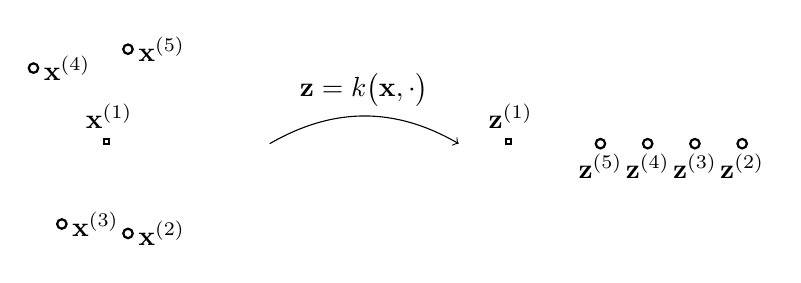
\begin{tikzpicture}[auto,scale=0.6]
        			% Left rectangle (\featurespace)
       			% \draw [thick] (-9,-3) rectangle (-2,4) node [anchor=east,above] {$\featurespace$};
        			\draw [thick] (-6,2) circle (0.1cm) node[anchor=west] {\hspace*{0mm}${\bf x}^{(5)}$};
       			\draw [thick] (-8,1.6) circle (0.1cm) node[anchor=west] {\hspace*{0mm}${\bf x}^{(4)}$};
        			\draw [thick] (-7.4,-1.7) circle (0.1cm) node[anchor=west] {\hspace*{0mm}${\bf x}^{(3)}$};
        			\draw [thick] (-6,-1.9) circle (0.1cm) node[anchor=west] {\hspace*{0mm}${\bf x}^{(2)}$};
        			\draw [thick] (-6.5,0.0) rectangle ++(0.1cm,0.1cm) node[anchor=west,above] {\hspace*{0mm}${\bf x}^{(1)}$};
			%
			%        % Right rectangle (\featurespace')
      			% \draw [thick] (0,-4) rectangle (7,3) node [anchor=east,above] {$\featurespace'$};
        			\draw [thick] (4,0) circle (0.1cm) node[anchor=north] {\hspace*{0mm}${\bf z}^{(5)}$};
        			\draw [thick] (5,0) circle (0.1cm) node[anchor=north] {\hspace*{0mm}${\bf z}^{(4)}$};
        			\draw [thick] (6,0) circle (0.1cm) node[anchor=north] {\hspace*{0mm}${\bf z}^{(3)}$};
        			\draw [thick] (7,0) circle (0.1cm) node[anchor=north] {\hspace*{0mm}${\bf z}^{(2)}$};
        			\draw [thick] (2,0) rectangle ++(0.1cm,0.1cm) node[anchor=west,above] {\hspace*{0mm}${\bf z}^{(1)}$};
			%
			%        % Arrow from left rectangle to right rectangle
       			\draw[->,bend left=30] (-3,0) to node[midway,above] {${\bf z}= k\big({\bf x},\cdot\big)$} (1,0);
    			\end{tikzpicture}
			\end{center}
		\caption{Five data points characterized by feature vectors ${\bf x}^{(r)}$ 
			and labels $y^{(r)} \in \{ \circ, \square \}$ for $r=1, \,\ldots, \,5$. 
			With these feature vectors, there is no way to separate the two classes 
			by a straight line (representing the decision boundary of a linear classifier). 
			In contrast, the transformed feature vectors ${\bf z}^{(r)} = k\big({\bf x}^{(r)},\cdot\big)$ 
			allow us to separate the data points using a linear classifier.  \label{fig_linsep_kernel_dict}}
		\end{figure}
		See also: kernel, feature vector, feature space, linear classifier.},
	first={kernel method},
	plural={kernel methods},
	text={kernel method} 
}
	
\newglossaryentry{cm}
{name={confusion matrix}, 
	description={Consider\index{confusion matrix} a finite dataset 
		with $m$ data points, each characterized 
		by a feature vector ${\bf x}$ and a label 
		$y\in \mathcal{Y}$ with a finite label space $\mathcal{Y}= \{1, \,\ldots, \,k\}$. 
		For a given hypothesis $h$, the confusion matrix is a 
		$k\times k$ matrix where each row corresponds 
		to a specific value of the true label $y\in \mathcal{Y}$ 
		and each column to a specific value of the prediction $h({\bf x}) \in \mathcal{Y}$. 
		The matrix entry in the $c$th row and $c'$th 
		column is the number of data points with the true label 
		$y= c$ that are predicted as 
		$h({\bf x}) = c'$. The sum of the main 
		diagonal entries is the number of correctly classified 
		data points, i.e., those for which $y= h({\bf x})$. 
		Summing the off-diagonal entries results in the total number of data points 
		that are misclassified by $h$.
				\\
		See also: label, label space, hypothesis, matrix, classification.},
	first={confusion matrix},
	text={confusion matrix} 
}

\newglossaryentry{precision}
{name={precision}, 
	description={Precision\index{precision} is a metric commonly used in binary classification for 
		the assessment of trained models. It measures the proportion of correctly 
		predicted data points among those with a positive label 
		\cite{Juba_Le_2019}, \cite{Rijsbergen1979}.
		\\
		See also: metric, classification, confusion matrix, recall.},
	first={precision}, 
	text={precision}
}

\newglossaryentry{recall}
{name={recall}, 
	description={Recall\index{recall} is a metric commonly used in binary classification for 
		the assessment of trained models. It is the ratio between the number of 
		true positives (i.e., correctly predicted positive data points) and the number 
		of data points with a positive label \cite{Juba_Le_2019}, \cite{Rijsbergen1979}.
		\\ 
		See also: metric, classification, confusion matrix, precision.},
	first={recall}, 
	text={recall}
}

\newglossaryentry{sensitivity}
{name={sensitivity}, 
	description={See\index{sensitivity} recall.},
	first={sensitivity}, 
	text={sensitivity}
}

\newglossaryentry{transferlearning}
{name={transfer learning},
	description={Transfer learning\index{transfer learning} aims at leveraging information 
		obtained while solving an existing learning task to 
   		solve another learning task.
		\\ 
   		See also: learning task, multitask learning},
  	first={transfer learning},
  	text={transfer learning}
}

\newglossaryentry{featuremtx}
{name={feature matrix}, 
	description={Consider\index{feature matrix} a dataset $\mathcal{D}$ 
		with $m$ data points with feature vectors 
		${\bf x}^{(1)}, \,\ldots, \,{\bf x}^{(m)} \in \mathbb{R}^{d}$. 
		It is convenient to collect the individual feature vectors into 
		the feature matrix:
		$${\bf X}:=\big({\bf x}^{(1)}, \,\ldots, \,{\bf x}^{(m)}\big)\,^{T} =
		\begin{pmatrix}
			x^{(1)}_{1} & x^{(1)}_{2} & \cdots & x^{(1)}_{d} \\
			x^{(2)}_{1} & x^{(2)}_{2} & \cdots & x^{(2)}_{d} \\
			\vdots      & \vdots      & \ddots & \vdots \\
			x^{(m)}_{1} & x^{(m)}_{2} & \cdots & x^{(m)}_{d}
		\end{pmatrix}
		\in \mathbb{R}^{m\times d}.$$
		Note that the feature matrix is of size $m\times d$, i.e., 
		it has $m$ rows and $d$ columns.
				\\
		See also: dataset, data point, feature vector, feature, matrix.},
	first={feature matrix},
	text={feature matrix} 
}

% \newglossaryentry{kmeans++}
% {name={$k$-means++}, 
%  description={$k$-means++ is a \gls{stochalgorithm} \index{$k$-means++} for constructing the 
%               initial \glspl{clustercentroid} in \gls{kmeans} methods such as \gls{lloydalgorithm} \cite{Arthur2007}.\\
% 		See also: \gls{kmeans}.},
%  first={$k$-means++},
%  text={$k$-means++} 
% }

\newglossaryentry{dbscan}
{name={density-based spatial clustering of applications with noise (DBSCAN)}, 
	description={DBSCAN\index{density-based spatial clustering of applications with noise (DBSCAN)} 
		refers to a clustering algorithm for data points that are characterized by numeric feature vectors. 
		Like $k$-means and soft clustering via Gaussian mixture model (GMM), DBSCAN also uses the Euclidean distances 
		between feature vectors to determine the clusters. However, in contrast to $k$-means 
		and Gaussian mixture model (GMM), DBSCAN uses a different notion of similarity between data points. 
		DBSCAN considers two data points as similar if they are connected 
		via a sequence (i.e., path) of nearby intermediate data points. Thus, DBSCAN might consider 
		two data points as similar (and therefore belonging to the same cluster) even if 
		their feature vectors have a large Euclidean distance.
				\\
		See also: clustering, $k$-means, Gaussian mixture model (GMM), cluster, graph.},
	first={density-based spatial clustering of applications with noise (DBSCAN)},
	text={DBSCAN} 
}

\newglossaryentry{fl}
{name={federated learning (FL)}, 
	description={FL\index{federated learning (FL)} 
		is an umbrella term for machine learning (ML) methods that train models in a collaborative 
		fashion using decentralized data and computation.
				\\
		See also: machine learning (ML), model, data.},
	first={federated learning (FL)},
	text={FL} 
}
	
\newglossaryentry{cfl}
{name={clustered federated learning (CFL)}, 
	description={CFL\index{clustered federated learning (CFL)} trains local models for the 
 		devices in an federated learning (FL) application by using a clustering assumption, i.e., the devices 
 		of an federated learning network (FL network) form clusters. Two devices in the same cluster generate 
 		local datasets with similar statistical properties. CFL pools the local datasets of devices 
 		in the same cluster to obtain a training set for a cluster-specific model. 
 		Generalized total variation minimization (GTVMin) clusters devices implicitly by enforcing approximate similarity of model parameters 
 		across well-connected nodes of the federated learning network (FL network).\\ 
 		See also: federated learning (FL), clustering assumption, federated learning network (FL network), cluster, graph clustering.},
	first={clustered federated learning (CFL)},
	text={CFL} 
}

\newglossaryentry{coreset}
{name={coreset}, 
	description={A coreset\index{coreset} is a small subset of a larger dataset 
		that approximates certain properties of the original dataset \cite{Chai2023}. 
		The construction of a coreset typically involves selecting representative data points
		and assigning them weights to reflect their importance in the original dataset (Fig.\ \ref{fig_coreset_dict}).
        		\begin{figure}[H]
			\centering
			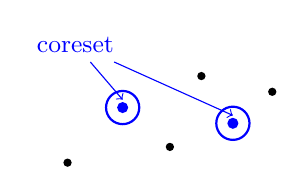
\begin{tikzpicture}
  			% all data points
  			\foreach \x/\y in {0.5/0.7, 1.2/1.4, 1.8/0.9, 2.2/1.8, 2.6/1.2, 3.1/1.6}
    			{\fill (\x,\y) circle (1.5pt);}
  			% coreset points (highlighted)
  			\foreach \x/\y in {1.2/1.4, 2.6/1.2}{
    			\fill[blue] (\x,\y) circle (2pt);
    			\draw[blue, thick] (\x,\y) circle (6pt);
  			}
  			% a simple label pointing to both coreset elements
  			\node[blue] (label) at (0.6,2.2) {\small coreset};
  			\draw[->,blue] (label) -- (1.2,1.5);
  			\draw[->,blue] (label) -- (2.6,1.3);
			\end{tikzpicture}
		\caption{A coreset (highlighted in blue) is a small subset of a larger dataset. \label{fig_coreset_dict}}
		\end{figure}
		Coresets are particularly useful for machine learning (ML) applications (such as clustering) 
		involving large datasets, as they allow for efficient computation while 
		preserving the essential characteristics of the data \cite{DistkmeansBalcan2013}.
				\\
		See also: dataset, data point, clustering.},
	first={coreset},
	firstplural={coresets},
	plural={coresets},
	text={coreset} 
}

\newglossaryentry{outlier}
{name={outlier}, 
	description={Many\index{outlier} machine learning (ML) methods 
		are motivated by the independent and identically distributed assumption (i.i.d.\ assumption), which interprets data points as realizations of 
		independent and identically distributed (i.i.d.) random variables (RVs) with a common probability distribution. The independent and identically distributed assumption (i.i.d.\ assumption) is useful for applications  
		where the statistical properties of the data generation process are stationary (or time-invariant) \cite{Brockwell91}. 
		However, in some applications, the data consist of a majority of regular data points 
		that conform with the independent and identically distributed assumption (i.i.d.\ assumption) as well as a small number of data points that have fundamentally different 
       		statistical properties compared with the regular data points. We refer to 
		a data point that substantially deviates from the statistical properties of 
		most data points as an outlier. Different methods for outlier detection 
		use different measures of this deviation. 
        		Statistical learning theory studies fundamental limits on the ability to 
		mitigate outliers reliably \cite{doi:10.1137/0222052}, \cite{10.1214/20-AOS1961}.
        		\\
		See also: robustness, stability, Huber regression, probabilistic model.},
	 first={outlier},
	 text={outlier} 
}

\newglossaryentry{membershipinferenceattack}
{name={membership inference attack}, 
	description={Consider an machine learning (ML) method that learns a hypothesis 
		via empirical risk minimization (ERM) on a training set. Membership inference\index{membership inference attack} 
                attack is a form of privacy attack where an adversary tries 
		to determine whether a particular data point was part 
		of the training set. The attacker typically queries 
		$\hat{h}$ with candidate feature vectors 
		${\bf x}^{(1)},\,\ldots,\,{\bf x}^{(B)}$, 
		and infers the membership status of a given data point 
		based on the predictions $\hat{h}\big({\bf x}^{(1)}\big),\,\ldots,
		\,\hat{h}\big({\bf x}^{(B)}\big)$ \cite{Shokri2017}.
		\\ 
		See also: attack, privacy attack.}, 
 	first={membership inference attack}, 
 	text={membership inference attack}
}

\newglossaryentry{machineunlearning}
{name={machine unlearning},
	description={Consider an machine learning (ML) method that learns a hypothesis $\hat{h}$ 
		via empirical risk minimization (ERM) on a training set $\mathcal{D}$. The learned hypothesis can 
		reveal information about $\mathcal{D}$, which is exploited by privacy attacks such as 
		model inversion. Machine unlearning\index{machine unlearning} refers to techniques that 
		modify $\hat{h}$, so that it is harder to infer properties of individual 
		data points in $\mathcal{D}$ \cite{cao2015unlearning}. Machine unlearning helps 
		to meet legal requirements for privacy protection in artificial intelligence systems (AI systems) \cite{GDPR2016}. 
		\\
	 	See also: model inversion, privacy protection, general data protection regulation (GDPR). },
	first={machine unlearning},
	text={machine unlearning}
}

% Shouldn't this be ensemble method?
\newglossaryentry{ensemble}
{name={ensemble}, 
	description={An ensemble method\index{ensemble} combines multiple 
		machine learning (ML) methods, each of those referred to as a base learner, 
		to improve overall performance. The base learners can be empirical risk minimization (ERM)-based 
        		using different choices for the loss, model, and training set. 
		By aggregating the predictions of base learners, ensemble methods can 
		often achieve better performance than any single base learner. The 
		aggregation can amount to averaging the predictions of base learners 
		(in regression) or using a majority vote (for classification methods). 
		\begin{figure}[H]
		\begin{center}
			\begin{tikzpicture}[
				scale=1.1, transform shape,
				node distance=11mm and 10mm,
				dataset/.style={draw, rounded corners, inner sep=2pt},
				learner/.style={draw, rounded corners,inner sep=2pt},
				op/.style={draw, circle, inner sep=1pt},
				flow/.style={->, >=latex},
				feedback/.style={->, >=latex, dashed, very thin},
				lab/.style={font=\scriptsize}
				]
				% --- Source dataset
				\node[dataset] (D) {$\mathcal{D}$};
				% --- Variant datasets (could be resample/reweight/transform)
				\node[dataset, below left=of D]  (D1) {\small $\widetilde{\mathcal{D}}^{(1)}$};
				\node[dataset, below=of D]       (D2) {\small $\widetilde{\mathcal{D}}^{(2)}$};
				\node[dataset, below right=of D] (D3) {\small $\widetilde{\mathcal{D}}^{(3)}$};
				\draw[flow] (D) -- (D1) node[midway, lab, above left=-1pt] {resample};
				\draw[flow] (D) -- (D2) node[midway, lab, right] {};
				\draw[flow] (D) -- (D3) node[midway, lab, above right=-1pt] {};
				% --- Base learners
				\node[learner, below=5mm of D1] (L1) {\small $\mathcal{H}^{(1)}$};
				\node[learner, below=5mm of D2] (L2) {\small $\mathcal{H}^{(2)}$};
				\node[learner, below=5mm of D3] (L3) {\small $\mathcal{H}^{(3)}$};
				% --- Data-to-learner edges
				\draw[flow] (D1) -- (L1);
				\draw[flow] (D2) -- (L2);
				\draw[flow] (D3) -- (L3);
				% --- Inter-learner dependencies (generic; like boosting-style feedback)
				\draw[feedback] (L1.east) .. controls +(+7mm,0mm) and +(-7mm,0mm) .. (L2.west)
				node[midway, lab, above] {};
				\draw[feedback] (L2.east) .. controls +(+7mm,0mm) and +(-7mm,0mm) .. (L3.west);
				% (Optional: allow skip connections)
				\draw[feedback] (L1.east) to[out=60, in=120] (L3.west);
				% --- Aggregator and final prediction
				\node[op, below=8mm of L2] (agg) {\small $\phi_{\text{agg}}$};
				\draw[flow] (L1) -- (agg);
				\draw[flow] (L2) -- (agg);
				\draw[flow] (L3) -- (agg);
				% --- Prediction display
				\node[below=5mm of agg, align=right, inner sep=2pt] (yhat)
				{\small $\hat{h}= \phi_{\text{agg}}\!\big(\widehat{h}^{(1)},\,\widehat{h}^{(2)},\,\widehat{h}^{(3)}\big)$};
				\draw[flow] (agg) -- (yhat);
				% --- Tiny labels on learner outputs
				\node[lab, below left=-1pt and -1pt of L1.south] {$\widehat{h}^{(1)}$};
				\node[lab, below           =-1pt of L2.south]    {$\widehat{h}^{(2)}$};
				\node[lab, below right=-1pt and -1pt of L3.south]{$\widehat{h}^{(3)}$};
				% --- Mini legend for dashed feedback
				%	\node[lab, above right=2mm and 0mm of L3] (leg) {dashed: inter-learner info};
				%	\draw[feedback] ($(leg.west)+(0mm,-1.5mm)$) -- ++(-8mm,0mm);
			\end{tikzpicture}
			\caption{A generic ensemble with three base learners, each  
				using empirical risk minimization (ERM) to learn $\mathcal{H}^{(j)} \in \mathcal{H}^{(j)}$ 
				based on the training set $\widetilde{\mathcal{D}}^{(j)}$. A base learner might also 
				use the output of other base learners. The final hypothesis $\hat{h}$ 
				is obtained by aggregating the hypotheses generated by the base learners.}
		\end{center}
		\end{figure}
		Different ensemble methods use different constructions for the base learners. 
		For example, bagging methods (such as a random forest) use random sampling to 
		construct slightly different training sets for each base learner. 
	    	On the other hand, boosting methods run the base learners 
		sequentially, i.e., each base learner tries to correct the prediction 
		errors of the previous ones. A third family of ensemble methods is stacking, 
		where base learners are trained on the same training set but with 
		different models.
		\\
	 	See also: bagging, boosting, stacking.},
	 first={ensemble},
	 text={ensemble} 
}

\newglossaryentry{stacking}
{name={stacking}, 
	description={Stacking\index{stacking} is one of the main types of ensemble methods.  
		In stacking, a finite number $M$ of base learners are trained on the 
		same dataset but with different models $\mathcal{H}^{(j)}$ 
		or loss functions $L^{(j)}$ for $j=1,\,\ldots,\,M$ \cite[Ch. 8.8]{hastie01statisticallearning},
		\cite{WOLPERT1992241}, \cite{ZhouEnsemble2012}. 
		The $j$th base learner delivers a learned hypothesis 
		$\widehat{h}^{(j)} \in \mathcal{H}^{(j)}$. 
		The final prediction for a data point is obtained by aggregating the 
		predictions of the base learners via an aggregation rule $\phi_{\rm agg}$, 
		such as majority voting for classification or averaging for regression. 
		We can interpret stacking as a form of feature learning, where each base learner 
		extracts a new feature. The aggregation rule can be obtained by another instance 
		of empirical risk minimization (ERM) that learns a hypothesis map $\phi_{\rm agg} \in \mathcal{H}$ from 
		a meta-model $\mathcal{H}$. The hypothesis $\phi_{\rm agg}$ is applied to the 
		transformed feature vector $${\bf \Phi}({\bf x})= \big( \hat{h}^{(1)}({\bf x}), 
       		\,\ldots, \,\hat{h}^{(M)}({\bf x}) \big)^{T}.$$
       		\begin{figure}[H]
			\begin{center}
			\begin{tikzpicture}[
			font=\small,
			scale=1.0, transform shape,
			node distance=7mm and 10mm,
			dataset/.style={draw, rounded corners, inner sep=2pt},
			learner/.style={draw, rounded corners, minimum width=14mm, minimum height=7mm, inner sep=6pt,align=center},
			op/.style={draw, circle, inner sep=1pt},
			>=latex
			]
			% Original dataset
			\node[dataset] (D) {$\mathcal{D}$};
			% Variants (closer to D)
			\node[learner, below left=of D]  (L1) {empirical risk minimization (ERM) \\ $\mathcal{H}^{(1)},L^{(1)}$};
			\node[learner, below=of D]       (L2) {empirical risk minimization (ERM) \\ $\mathcal{H}^{(2)},L^{(2)}$};
			\node[learner, below right=of D] (L3) {empirical risk minimization (ERM) \\ $\mathcal{H}^{(3)},L^{(3)}$};
			% Arrows to variants (shorter labels)
			\draw[->] (D) -- (L1) node[midway, above left=-1pt] {};
			\draw[->] (D) -- (L2) node[midway, right]           {};
			\draw[->] (D) -- (L3) node[midway, above right=-1pt]{};
			\node[op, below=8mm of L2] (agg) {$\phi_{\text{agg}}$};
			\node[below=5mm of agg, align=right, inner sep=2pt] (yhat)
			{$\hat{y}= \phi_{\text{agg}}\!\big(\widehat{h}^{(1)}({\bf x}),\widehat{h}^{(2)}({\bf x}),\widehat{h}^{(3)}({\bf x})\big)$};
			\draw[->] (L1) -- (agg);
			\draw[->] (L2) -- (agg);
			\draw[->] (L3) -- (agg);
			\draw[->] (agg) -- (yhat);
			% Tiny labels on learner outputs
			\node[below left=-1pt and -1pt of L1.south] {$\widehat{h}^{(1)}$};
			\node[below           =-1pt of L2.south]    {$\widehat{h}^{(2)}$};
			\node[below right=-1pt and -1pt of L3.south]{$\widehat{h}^{(3)}$};
			\end{tikzpicture}
		\caption{Three base learners using empirical risk minimization (ERM) with 
			different models and loss functions to obtain learned hypotheses 
			$\widehat{h}^{(1)},\,\widehat{h}^{(2)},\,\widehat{h}^{(3)}$. 
			For a data point with feature vector ${\bf x}$, each base learner delivers a prediction  
			$\widehat{h}^{(j)}({\bf x})$ for $j=1,\,2,\,3$. These 
			predictions are then used as new features for an aggregation 
			rule $\phi_{\rm agg}$ that delivers the overall prediction $\hat{y}$. 
			The aggregation rule can be obtained by training a meta-model $\mathcal{H}$.}
			\end{center}
		\end{figure}
	 	See also: ensemble, bagging.},
	 first={stacking},
	 text={stacking} 
}

\newglossaryentry{auc}
{name={area under the curve (AUC)}, 
	description={The AUC\index{area under the curve (AUC)} is a quantitative measure of the 
 		usefulness of a binary classifier \cite{Hanley:1982aa}. It 
		is defined (using the natural measure of the Euclidean space $\mathbb{R}^{2}$) as the area  
		under the receiver operating characteristic (ROC) curve.
		\\
		See also: classifier, Euclidean space, receiver operating characteristic (ROC). } , 
 	first={area under the curve (AUC)}, 
 	text={AUC} 
}

\newglossaryentry{roc} 
{name={receiver operating characteristic (ROC)}, 
	description={Consider a label space $\mathcal{Y}=\{-1,1\}$ and a classifier 
 		that uses a real-valued hypothesis $h({\bf x})$. For a given 
 		threshold $\eta \in \mathbb{R}$, the ultimate prediction is $\hat{y}=1$ 
 		if $h({\bf x})\geq \eta$ and $\hat{y}=-1$ otherwise. 
 		On a test set $\mathcal{D}^{(\rm test)} $, we compute, for each value of $\eta$, 
		the following two quantities: 1) true positive rate ${\rm TPR}^{(\eta)}$; 
		and 2) false positive rate ${\rm FPR}^{(\eta)}$. 
 		The ROC curve\index{receiver operating characteristic (ROC)} is  
 		the following function \cite{IntroROCFawcett}:
 		$${\rm ROC}: \mathbb{R} \rightarrow \mathbb{R}^{2}: \eta \mapsto \big({\rm TPR}^{(\eta)}, {\rm FPR}^{(\eta)} \big).$$ 
 	        One important characteristic of the ROC curve is the area under the curve (AUC).
	        \\ 
 		See also: classifier, area under the curve (AUC).}, 
  	first={receiver operating characteristic (ROC)}, 
  	text={ROC}
}

\newglossaryentry{bagging}
{name={bagging},
	description={Bagging\index{bagging} is an ensemble technique where base learners 
		use perturbed copies $$\widetilde{\mathcal{D}}^{(1)},\,\ldots,\,\widetilde{\mathcal{D}}^{(M)}$$ 
		of the original training set $\mathcal{D}$ \cite{Breiman:1996aa}. Each 
		base learner delivers a potentially different hypothesis $$\hat{h}^{(1)},\,\ldots,\,\hat{h}^{(M)}.$$
		The hypothesis delivered by the overall method is obtained by 
		aggregating the hypotheses $\hat{h}^{(1)},\,\ldots,\,\hat{h}^{(M)}$ 
		using some aggregation rule. For classification methods, the rule is typically 
		a majority vote, while for regression methods, it amounts to averaging. 
		\begin{figure}[H]
			\begin{center}
			\begin{tikzpicture}[
			scale=1.0, transform shape,
			node distance=10mm and 10mm,
			dataset/.style={draw, rounded corners, inner sep=2pt},
			learner/.style={draw, rounded corners, minimum width=14mm, minimum height=7mm, inner sep=2pt},
			op/.style={draw, circle, inner sep=1pt},
			>=latex
			]
			% Original dataset
			\node[dataset] (D) {$\mathcal{D}$};
			% Variants (closer to D)
			\node[dataset, below left=of D]  (D1) {$\widetilde{\mathcal{D}}^{(1)}$};
			\node[dataset, below=of D]       (D2) {$\widetilde{\mathcal{D}}^{(2)}$};
			\node[dataset, below right=of D] (D3) {$\widetilde{\mathcal{D}}^{(3)}$};
			% Arrows to variants (shorter labels)
			\draw[->] (D) -- (D1) node[midway, above left=-1pt] {resample};
			\draw[->] (D) -- (D2) node[midway, right]           {resample};
			\draw[->] (D) -- (D3) node[midway, above right=-1pt]{resample};
			% Base learners (reduced vertical gaps)
			\node[learner, below=5mm of D1] (L1) {$\mathcal{H}^{(1)}$};
			\node[learner, below=5mm of D2] (L2) {$\mathcal{H}^{(2)}$};
			\node[learner, below=5mm of D3] (L3) {$\mathcal{H}^{(3)}$};
			% Feed variants into learners
			\draw[->] (D1) -- (L1);
			\draw[->] (D2) -- (L2);
			\draw[->] (D3) -- (L3);
			% Aggregator and final prediction (tighter)
			\node[op, below=8mm of L2] (agg) {$\phi_{\text{agg}}$};
			\node[below=5mm of agg, align=right, inner sep=2pt] (yhat)
			{$\hat{h}= \phi_{\text{agg}}\!\big(\widehat{h}^{(1)},\widehat{h}^{(2)},\widehat{h}^{(3)}\big)$};
			\draw[->] (L1) -- (agg);
			\draw[->] (L2) -- (agg);
			\draw[->] (L3) -- (agg);
			\draw[->] (agg) -- (yhat);
			% Tiny labels on learner outputs
			\node[below left=-1pt and -1pt of L1.south] {$\widehat{h}^{(1)}$};
			\node[below           =-1pt of L2.south]    {$\widehat{h}^{(2)}$};
			\node[below right=-1pt and -1pt of L3.south]{$\widehat{h}^{(3)}$};
			\end{tikzpicture}
		\caption{An example of bagging where three base learners use perturbations  
			$\widetilde{\mathcal{D}}^{(1)},\,\ldots,\,\widetilde{\mathcal{D}}^{(3)}$ of 
			the original training set $\mathcal{D}$ to learn the hypotheses 
			$\widehat{h}^{(1)},\,\ldots,\,\widehat{h}^{(3)}$. The final 
			hypothesis is obtained by aggregating these individual hypotheses 
			via some aggregation rule $\phi_{\rm agg}$.}
			\end{center}
		\end{figure}
		See also: ensemble, robustness, bootstrap.},
	first={bagging},
	text={bagging}
}

\newglossaryentry{bootstrap aggregation}
{name={bootstrap aggregation}, 
	description={See bagging\index{bootstrap aggregation}.},
 	first={bootstrap aggregation},
 	text={bootstrap aggregation} 
}	

\newglossaryentry{decisionregion}
{name={decision region},
	description={Consider\index{decision region} 
		a hypothesis map $h$ that delivers values from a finite set $\mathcal{Y}$. 
		For each label value (i.e., category) $a \in \mathcal{Y}$, the hypothesis $h$ 
		determines a subset of feature values ${\bf x}\in \mathcal{X}$ that result 
		in the same output $h({\bf x})=a$. We refer to this subset as a decision 
		region of the hypothesis $h$. 
		\\
		See also: hypothesis, map, label, feature.},
	first={decision region},
	plural={decision regions}, 
	firstplural={decision regions}, 
	text={decision region} 
}

\newglossaryentry{baselearner}
{name={base learner}, 
	description={A base learner\index{base learner} is an machine learning (ML) method 
         	that is part of an ensemble method. 
		\\
		See also: ensemble, bagging, stacking, boosting.},
	first={base learner},
	firstplural={base learners},
	plural={base learners},
	text={base learner} 
}	

\newglossaryentry{decisionboundary}
{name={decision boundary}, 
	description={Consider\index{decision boundary} a 
		hypothesis map $h$ that reads in a feature vector  
		${\bf x}\in \mathbb{R}^{d}$ and delivers a value from a finite set $\mathcal{Y}$. 
		The decision boundary of $h$ is the set of vectors ${\bf x}\in \mathbb{R}^{d}$ 
		that lie between different decision regions. More precisely, a 
		vector ${\bf x}$ belongs to the decision boundary if and only 
		if each neighborhood $\{ {\bf x}': \| {\bf x}- {\bf x}' \| \leq \varepsilon \}$, 
		for any $\varepsilon >0$, contains at least two vectors with different function values.
				\\
		See also: hypothesis, map, feature vector, boundary, vector, decision region, 
		neighborhood, function.},
	first={decision boundary},
	firstplural={decision boundaries},
	plural={decision boundaries},
	text={decision boundary} 
}

\newglossaryentry{normalequations}
{name={normal equations}, 
	description={Consider linear least squares\index{normal equations}, which learns the parameters of a 
		linear model by minimizing the average squared error loss on a 
		training set $\mathcal{D}$. 
		The learned parameters $\widehat{{\bf w}}$ are characterized by the 
		linear system of equations, i.e.,
		\begin{equation} 
			\label{equ_normal_equations_dict}
			{\bf X}^{T} {\bf X}\widehat{{\bf w}} = {\bf X}^{T} {\bf y}.
		\end{equation} 
		Here, ${\bf X}=\big({\bf x}^{(1)},\,\ldots,\,{\bf x}^{(m)}\big)^{T} \in \mathbb{R}^{m\times d}$ 
		is the feature matrix of $\mathcal{D}$ and ${\bf y}=\big(y^{(1)},\,\ldots,\,y^{(m)} \big)^{T} \in \mathbb{R}^{m}$ 
		is the label vector of $\mathcal{D}$. This linear system of equations is referred 
		to as normal equations, as it amounts to an orthogonality condition. Indeed, \eqref{equ_normal_equations_dict} 
		can be rewritten as $$ {\bf X}^{T} \big( {\bf X}\widehat{{\bf w}} - {\bf y}\big) = \mathbf{0}.$$
		This means that the prediction error vector ${\bf X}\widehat{{\bf w}} - {\bf y}$ 
		is orthogonal to the columns of ${\bf X}$ and, in turn, to the subspace ${\rm span}\left({\bf X}\right)$
		spanned by them.
		\\ 
		See also: linear least squares, model parameter. },
	first={normal equations},
	text={normal equations} 
}

\newglossaryentry{eerm}
{name={explainable empirical risk minimization (EERM)}, 
	description={EERM is an\index{explainable empirical risk minimization (EERM)} 
		in-\linebreak stance of structural risk minimization (SRM) that adds a regularization term to the 
		average loss in the objective function of empirical risk minimization (ERM). 
		The regularization term is chosen to favor hypothesis maps that are intrinsically 
		explainable for a specific user. This user is characterized by their predictions provided 
		for the data points in a training set \cite{Zhang:2024aa}.
				\\
		See also: structural risk minimization (SRM), regularization, empirical risk minimization (ERM), training set.},
	first={explainable empirical risk minimization (EERM)},
	text={EERM} 
}
	
\newglossaryentry{kmeans}
{name={$k$-means}, 
sort={k-means},
	description={The\index{$k$-means} $k$-means principle is an optimization-based 
	    	approach to the clustering of data points with a numeric feature vector \cite[Ch. 8]{MLBasics}. 
		As a hard clustering approach, $k$-means partitions a dataset into $k$ disjoint 
		subsets (or clusters), which are indexed by $c=1,\,\ldots,\,k$. Each cluster $\mathcal{C}$ 
		is characterized by the average feature vector of data points that belong to it. This average 
		(or mean) feature vector is referred to as the cluster centroid ${{\bf w}}^{(c)}$. 
		A visual illustration is provided in Fig. \ref{fig_kmeans_dict}.
		\begin{figure}[H]
		\begin{center}
		\begin{tikzpicture}[scale=1]
			% Styles
			\tikzset{
			data/.style={circle, fill=black, inner sep=1.2pt},
			centroid/.style={thick, cross out, draw, minimum size=6pt, inner sep=0pt}
			}
			% Cluster A data (with one labeled point)
			\node[data] (xi) at (1.0,0.2) {};
			\node[right=0pt of xi,yshift=2pt] {${\bf x}^{(r)}$};
			% The rest unlabeled
			\foreach \p in {(-0.3,0.0),(0.2,-0.4),(0.6,0.8),(0.0,0.9),(1.1,-0.2)}
			\node[data] at \p {};
			% Cluster B data (spread wider)
			\foreach \p in {(2.5,1.0),(3.7,1.2),(2.6,2.3),(3.8,2.5),(3.0,2.9),(3.6,1.6)}
			\node[data] at \p {};
			% Centroids as crosses
			\node[centroid] (mu1) at (0.55,0.4) {};
			\node[centroid] (mu2) at (3.1,1.85) {};
			% Labels
			\node[above of=mu1,yshift=-25pt,xshift=-10pt] {${{\bf w}}^{(1)}$};
			\node[above of=mu2,yshift=-25pt,xshift=-10pt] {${{\bf w}}^{(2)}$};
		\end{tikzpicture}
		\end{center}
		\caption{A scatterplot of data points, indexed by $r=1,\,\ldots,\,m$ and 
			characterized by feature vectors ${\bf x}^{(r)} \in \mathbb{R}^{2}$. 
			The scatterplot also includes two cluster centroids ${{\bf w}}^{(1)}, {{\bf w}}^{(2)} \in \mathbb{R}^{2}$. \label{fig_kmeans_dict}}
		\end{figure} 
		In general, solving the $k$-means optimization problem exactly is challenging (or NP-hard) 
		\cite{Mahajan2009Springer}. However, there are simple iterative methods for finding 
		approximately optimal cluster centroids. One such method is referred to as 
		Lloyd's algorithm.
		\\
		See also: hard clustering, cluster, Lloyd's algorithm.},
	first={$k$-means},
	text={$k$-means} 
}

\newglossaryentry{lloydalgorithm} 
{name={Lloyd's algorithm}, 
	description={Lloyd's\index{Lloyd's algorithm} algorithm \cite{Lloyd1982} is an iterative 
		optimization method for finding cluster centroids that are approximately 
	   	optimal for the $k$-means objective function. Lloyd's algorithm  
	   	alternates between: 1) updating the cluster assignment of each data point 
		based on the nearest current cluster centroid; and 
		2) recalculating the cluster centroids given the updated 
		cluster assignments \cite{Lloyd1982}.
		\begin{figure}[H]
			\begin{center}
			\begin{tikzpicture}[
			assignment/.style={-Latex, very thin},
			move/.style={-Latex, thick},
			center/.style={draw, circle, inner sep=1.2pt, fill=white},
			pointA/.style={circle, inner sep=1.1pt, fill=black},
			pointB/.style={rectangle, inner sep=1.1pt, fill=black},
			cross/.style={line width=0.4pt},
			lab/.style={font=\scriptsize}
			]
			% ===================== PANEL (a): Initial centers =====================
			% ===================== PANEL (b): Assign to nearest =====================
			\begin{scope}[shift={(0,0)}]
				% points
				\coordinate (Ba1) at (0.2, 1.1);
				\coordinate (Ba2) at (0.4, 0.6);
				\coordinate (Ba3) at (0.8, 1.0);
				\coordinate (Ba4) at (0.6, 0.2);
				\coordinate (Bb1) at (2.7, 1.4);
				\coordinate (Bb2) at (3.2, 0.9);
				\coordinate (Bb3) at (2.6, 0.3);
				\coordinate (Bb4) at (3.3, 0.2);
				\node[pointA] at (Ba1) {}; \node[pointA] at (Ba2) {}; \node[pointA] at (Ba3) {}; \node[pointA] at (Ba4) {};
				\node[pointB] at (Bb1) {}; \node[pointB] at (Bb2) {}; \node[pointB] at (Bb3) {}; \node[pointB] at (Bb4) {};
				% centers (old)
				\coordinate (Bc1old) at (0.9,0.65);
				\coordinate (Bc2old) at (2.8,1.8);
				\node[center,label={[lab, xshift=-2pt]right:${{\bf w}}^{(1,t)}$}] (B-C1) at (Bc1old) {};
				\node[center,label={[lab, xshift=-2pt]right:${{\bf w}}^{(2,t)}$}] (B-C2) at (Bc2old) {};
				% perpendicular bisector
				\path let 
				\p1=(B-C1), \p2=(B-C2),
				\n1={(\x2-\x1)}, \n2={(\y2-\y1)},
				\n3={veclen(\n1,\n2)}
				in coordinate (B-M)    at ($ (B-C1)!0.5!(B-C2) $)
				coordinate (B-Nhat) at ($ (0,0) + ({-\n2/\n3},{\n1/\n3}) $);
				\draw[dashed, thick] ($ (B-M) + 10.4*(B-Nhat) $) -- ($ (B-M) - 10.4*(B-Nhat) $);
				% minimal assignment spokes
				\draw[assignment] (Ba2) -- (B-C1);
				\draw[assignment] (Ba3) -- (B-C1);
				\draw[assignment] (Bb2) -- (B-C2);
				\draw[assignment] (Bb3) -- (B-C2);
				\node[lab] at (1.6,-0.35) {Assign to the nearest cluster centroid.};
				\node at (1.6,-1.3) {(a)};
			\end{scope}
			% ===================== PANEL (c): Recompute means =====================
			\begin{scope}[shift={(5.5,0)}]
				% points
				\coordinate (Ca1) at (0.2, 1.1);
				\coordinate (Ca2) at (0.4, 0.6);
				\coordinate (Ca3) at (0.8, 1.0);
				\coordinate (Ca4) at (0.6, 0.2);
				\coordinate (Cb1) at (2.7, 1.4);
				\coordinate (Cb2) at (3.2, 0.9);
				\coordinate (Cb3) at (2.6, 0.3);
				\coordinate (Cb4) at (3.3, 0.2);
				\node[pointA] at (Ca1) {}; \node[pointA] at (Ca2) {}; \node[pointA] at (Ca3) {}; \node[pointA] at (Ca4) {};
				\node[pointB] at (Cb1) {}; \node[pointB] at (Cb2) {}; \node[pointB] at (Cb3) {}; \node[pointB] at (Cb4) {};
				% centers (old and new)
				\coordinate (Cc1old) at (0.9,0.65);
				\coordinate (Cc2old) at (2.8,1.8);
				\coordinate (Cc1new) at (0.5,0.725);
				\coordinate (Cc2new) at (2.95,0.70);
				\node[center, opacity=0.5] at (Cc1old) {};
				\node[center, opacity=0.5] at (Cc2old) {};
				% crosses for new centers
				\draw[cross] ($(Cc1new)+(-0.07,0)$) -- ($(Cc1new)+(0.07,0)$);
				\draw[cross] ($(Cc1new)+(0,-0.07)$) -- ($(Cc1new)+(0,0.07)$);
				\draw[cross] ($(Cc2new)+(-0.07,0)$) -- ($(Cc2new)+(0.07,0)$);
				\draw[cross] ($(Cc2new)+(0,-0.07)$) -- ($(Cc2new)+(0,0.07)$);
				% movement arrows
				\draw[move] (Cc1old) -- (Cc1new);
				\draw[move] (Cc2old) -- (Cc2new);
				\node[lab] at (1.6,-0.35) {Recompute cluster centroids.};
				\node at (1.6,-1.3) {(b)};
			\end{scope}
			% ===================== PANEL (d): Update & new partition =====================
			\begin{scope}[shift={(3,-4)}]
				% points
				\coordinate (Da1) at (0.2, 1.1);
				\coordinate (Da2) at (0.4, 0.6);
				\coordinate (Da3) at (0.8, 1.0);
				\coordinate (Da4) at (0.6, 0.2);
				\coordinate (Db1) at (2.7, 1.4);
				\coordinate (Db2) at (3.2, 0.9);
				\coordinate (Db3) at (2.6, 0.3);
				\coordinate (Db4) at (3.3, 0.2);
				\node[pointA] at (Da1) {}; \node[pointA] at (Da2) {}; \node[pointA] at (Da3) {}; \node[pointA] at (Da4) {};
				\node[pointB] at (Db1) {}; \node[pointB] at (Db2) {}; \node[pointB] at (Db3) {}; \node[pointB] at (Db4) {};
				% centers (new)
				\coordinate (Dc1new) at (0.5,0.725);
				\coordinate (Dc2new) at (2.95,0.70);
				\node[center, label={[lab, xshift=-2pt]right:${{\bf w}}^{(1,t+1)}$}] (D-C1n) at (Dc1new) {};
				\node[center, label={[lab]right:${{\bf w}}^{(2,t+1)}$}] (D-C2n) at (Dc2new) {};
				% perpendicular bisector
				\path let 
				\p1=(D-C1n), \p2=(D-C2n),
				\n1={(\x2-\x1)}, \n2={(\y2-\y1)},
				\n3={veclen(\n1,\n2)}
				in coordinate (D-M)    at ($ (D-C1n)!0.5!(D-C2n) $)
				coordinate (D-Nhat) at ($ (0,0) + ({-\n2/\n3},{\n1/\n3}) $);
				\draw[dashed, thick] ($ (D-M) + 10.4*(D-Nhat) $) -- ($ (D-M) - 10.4*(D-Nhat) $);
				\node[lab] at (1.6,-0.35) {Assign to the nearest cluster centroid.};
				\node at (1.6,-1.3) {(c)};
			\end{scope}
			\end{tikzpicture}
			\end{center}
		\caption{Lloyd's algorithm alternates between (a) and (c) assigning data points to 
			the nearest cluster centroid and, in turn, (b) recomputing the cluster centroids 
			based on the new cluster assignments. 
			\label{fig_lloyd_algorithm_dict}}
		\end{figure}
		See also: cluster centroid, $k$-means, clustering.},
	first={Lloyd's algorithm},
	text={Lloyd's algorithm} 
}

\newglossaryentry{qlearning} 
{name={Q-learning}, 
	description={Q-learning\index{Q-learning} is a popular reinforcement learning (RL) 
	     	algorithm that learns an optimal policy by estimating the optimal action-value 
		function (or Q-function) \cite{SuttonEd2}.  
		\\
		See also: reinforcement learning (RL), fixed-point iteration.},
	first={Q-learning},
	text={Q-learning} 
}

\newglossaryentry{iteration}
{name={iteration},
	description={The elementary computational step during the execution of an 
		algorithm is referred to as iteration\index{iteration} 
		\cite{Cormen:2022aa}, \cite{KleinbergTardos2006}. 
		For example, the elementary computational step of gradient-based methods 
		is a gradient step. 
		More generally, the elementary computational step of a fixed-point iteration 
		is the evaluation of an underlying operator $\mathcal{F}$, which might 
		vary across iterations (see Fig. \ref{fig_iteration_dict}). 
		Many important machine learning (ML) algorithms, including 
		Lloyd's algorithm and gradient descent (GD), are fixed-point iterations.  
		\begin{figure}[H]
			\centering
			\begin{tikzpicture}[>=Latex, font=\small,scale=1]
			% --- baseline axis (purely visual) ---
			%			\draw[very thin] (-0.2,0) -- (5.6,0);
			% --- fixed point ---
			\node[circle,draw,inner sep=1.2pt,fill=white,label={above:${\bf w}^\ast$}] (xstar) at (8,0) {};
			% --- iterates ---
			\node[circle,fill,inner sep=1pt,label={below:${\bf w}^{(0)}$}] (x0) at (0.3,0) {};
			\node[circle,fill,inner sep=1pt,label={below:${\bf w}^{(1)}$}] (x1) at (4.3,0) {};
			\node[circle,fill,inner sep=1pt,label={below:${\bf w}^{(2)}$}] (x2) at (6.5,0) {};
			% --- update arrows labelled by the update operator T ---
			\draw[->] (x0) to[bend left=12] node[above,sloped] {$\mathcal{F}$} (x1);
			\draw[->] (x1) to[bend left=12] node[above,sloped] {$\mathcal{F}$} (x2);
			%\draw[->] (x5) to[bend left=12] node[above,sloped] {$\fixedpointop$} (xstar);
			% --- optional tiny stopping rule (comment out if too much) ---
			% \node[below=4pt of x4] {$\|x^{(t+1)} - x^{(t)}\| < \varepsilon$};
			\end{tikzpicture}
		\caption{A fixed-point iteration consists of the repeated application of an 
			operator $\mathcal{F}$ with some fixed point ${\bf w}^\ast$, i.e., 
			$\mathcal{F}{\bf w}^\ast={\bf w}^\ast$. \label{fig_iteration_dict}}
		\end{figure} 
		See also: algorithm, gradient step, gradient descent (GD).  },
	first={iteration},
	text={iteration},
	firstplural={iterations},
	plural={iterations}
}

\newglossaryentry{clustercentroid}
{name={cluster centroid}, 
	description={Clustering methods\index{cluster centroid} decompose a given 
		dataset into a few clusters. Different clustering methods use 
		different representations for these clusters. If data points are 
		characterized by numerical feature vectors ${\bf x}\in \mathbb{R}^{d}$, 
		we can use some vector ${\bm \mu} \in \mathbb{R}^{d}$, referred to 
		as cluster centroid, to represent a cluster. For example, if a cluster 
		consists of a set of data points, we use the average of their feature vectors 
		as a cluster centroid. However, there are also other choices for how to construct 
		a cluster centroid, e.g., using the geometric median (GM) \cite{PARK20093336} 
		or via non-Euclidean geometry \cite{JMLR:v6:banerjee05b}.
		\\
		See also: clustering, feature vector, $k$-means.},
	first={cluster centroid},
	firstplural={cluster centroids}, 
	text={cluster centroid}, 
	plural={cluster centroids}
}

\newglossaryentry{xml}
{name={explainable machine learning (XML)}, 
	description={XML\index{explainable machine learning (XML)} 
		methods aim to complement each prediction with an explanation of 
		how the prediction has been obtained. The construction of an explicit explanation 
		might not be necessary if the machine learning (ML) method uses a sufficiently simple (or interpretable) model \cite{rudin2019stop}.
				\\
		See also: prediction, explanation, machine learning (ML), model.},
	first={explainable machine learning (XML)},
	text={XML} 
}

\newglossaryentry{fmi}
{name={Finnish Meteorological Institute (FMI)}, 
	description={The\index{Finnish Meteorological Institute (FMI)}
		FMI is a government agency responsible for gathering 
		and reporting weather data in Finland.
				\\
		See also: data.},
	first={Finnish Meteorological Institute (FMI)},
	text={FMI} 
}
	
\newglossaryentry{samplemean}
{name={sample mean}, 
	description={The\index{sample mean} sample mean 
		${\bf m}\in \mathbb{R}^{d}$ for a given dataset, with feature vectors 
		${\bf x}^{(1)}, \,\ldots, \,{\bf x}^{(m)} \in \mathbb{R}^{d}$, is defined as 
		$${\bf m}= \frac{1}{m} \sum_{r=1}^{m} {\bf x}^{(r)}.$$ 
					\\
		See also: sample, mean, dataset, feature vector.},
	first={sample mean},
	text={sample mean} 
}
	
\newglossaryentry{highdimregime}
{name={high-dimensional regime}, 
	description={The\index{high-dimensional regime} 
		high-dimensional regime of empirical risk minimization (ERM) is characterized by the effective dimension of the model 
		being larger than the sample size, i.e., the number of (labeled) data points in the training set. 
		For example, linear regression methods operate in the high-dimensional regime whenever the number $d$ of features 
		used to characterize data points exceeds the number of data points in the training set. 
		Another example of machine learning (ML) methods that operate in the high-dimensional regime is large ANNs, which have 
		far more tunable weights (and bias terms) than the total number of data points in the training set. 
		High-dimensional statistics is a recent main thread of probability theory that studies the 
		behavior of machine learning (ML) methods in the high-dimensional regime \cite{Wain2019}, \cite{BuhlGeerBook}.
				\\
		See also: empirical risk minimization (ERM), effective dimension, overfitting, regularization.},
   	first={high-dimensional regime},
	text={high-dimensional regime} 
}

\newglossaryentry{gmm}
{name={Gaussian mixture model (GMM)}, 
	description={A GMM\index{Gaussian mixture model (GMM)} is a probabilistic model 
		for (the generation of) data points with numeric feature vectors 
		${\bf x}\in \mathbb{R}^d$ \cite{BishopBook}, \cite{Murphy2012}. 
		It assumes that each data point is generated by first drawing 
		a latent cluster index $I \in \{1,\,\ldots,\,k\}$
		according to cluster probabilities 
		$$\mathbb{P}\left(I=c\right) = p_{c}, 
		\qquad 
		\sum_{c=1}^{k} p_{c}=1.$$
		Conditioned on $I=c$, the feature vector ${\bf x}$ 
		is drawn from a multivariate normal distribution
		$\mathbb{P}^{(c)}= \mathcal{N}\left({\bm \mu}^{(c)},\mathbf{C}^{(c)}\right)$.
		The resulting marginal distribution of ${\bf x}$ is therefore 
		a weighted sum of multivariate normal distributions, i.e.,
		$$\mathbb{P}=\sum_{c=1}^{k}
		p_{c} \mathcal{N}\left({\bm \mu}^{(c)},\mathbf{C}^{(c)}\right).$$
		\begin{figure}[H]
		\begin{center}
		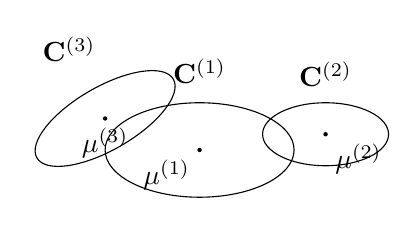
\begin{tikzpicture}[scale=0.4]
			% First component
			\draw (0,0) ellipse (3 and 1.5);
			\fill (0,0) circle (2pt);
			\node[below left] at (0,0) {${\bm \mu}^{(1)}$};
			\node[above] at (0,1.8) {$\mathbf{C}^{(1)}$};
			% Second component
			\draw (4,0.5) ellipse (2 and 1);
			\fill (4,0.5) circle (2pt);
			\node[below right] at (4,0.5) {${\bm \mu}^{(2)}$};
			\node[above] at (4,1.7) {$\mathbf{C}^{(2)}$};
			% Third (rotated) component
			\begin{scope}[rotate around={30:(-3,1)}]
			\draw (-3,1) ellipse (2.5 and 1);
			\end{scope}
			\fill (-3,1) circle (2pt);
			\node[below] at (-3,1) {${\bm \mu}^{(3)}$};
			\node[above left] at (-3,2.5) {$\mathbf{C}^{(3)}$};
		\end{tikzpicture}
		\caption{Illustration of a GMM with three components. \label{fig_gmm_dict}}
		\end{center}
		\end{figure}
				%   \begin{figure}[H]
				%  	\begin{tikzpicture}[scale=0.4]
				%  		\draw [thick] \boundellipse{0,0}{10}{5} node[right]  {$\meanvec{1}$};
				%  		\fill (0,0) circle (2pt) ; 
				%  		\node [right] at (0,5.5) {$\covmtx{1}$} ; 
				%  		\draw [thick] \boundellipse{11,1}{-2}{4} node[right]  {$\meanvec{2}$};
				%  		\fill (11,1) circle (2pt) ; 
				% 		\node [right] at (11,5.5) {$\covmtx{2}$} ; 
				% 		\draw [thick] \boundellipse{-9,4}{2}{3} 
				% 		node[left,xshift=3mm,yshift=3mm] {$\meanvec{3}$}; 
				% 		\fill (-9,4) circle (2pt) ; 
				% 		\node [right] at (-9,8) {$ \covmtx{3}$} ; 
				%	\end{tikzpicture}
				% 	\caption{Illustration of a GMM with three components.} 
				%Each component is a \glspl{mgvndist} 
				%         $\mvnormal{\meanvec{\clusteridx}}{\covmtx{\clusteridx}}$ with \gls{mean} 
				%			 \gls{vector} $\meanvec{\clusteridx}$ and \gls{covmtx} $\covmtx{\clusteridx}$. 
				% 	         The overall \gls{probdist} is a \gls{convex} combination of these 
				% 			 components, weighted by the \gls{cluster} \glspl{probability} $p_{\clusteridx}$.}
				% \end{figure}
		A GMM is parameterized by the cluster-specific probability  
		$p_{c}$, mean ${\bm \mu}^{(c)}$, and covariance matrix  
		$\mathbf{C}^{(c)}$ for $c=1,\,\ldots,\,k$.
		\\		
		See also: probabilistic model, multivariate normal distribution, clustering.},
	first={Gaussian mixture model (GMM)},
	plural={GMMs}, 
	firstplural={Gaussian mixture models (GMMs)}, 
	text={GMM} 
}


	
\newglossaryentry{polyreg}
{name={polynomial regression}, 
	description={Polynomial\index{polynomial regression} 
		regression is an instance of empirical risk minimization (ERM) that learns a polynomial hypothesis 
		map to predict a numeric label based on the numeric features of a data point. 
		 For data points characterized by a single numeric feature, polynomial regression uses the hypothesis space 
		$\mathcal{H}^{(\rm poly)}_{d} :=\{ h(x) = \sum_{j=0}^{d-1} x^{j} \weight_{j} \}.$
		The quality of a polynomial hypothesis map is measured using the average squared error loss 
		incurred on a set of labeled data points (which we refer to as the training set).
					\\
		See also: regression, empirical risk minimization (ERM), squared error loss.},
	first={polynomial regression},
	text={polynomial regression}
}

\newglossaryentry{leastsquares}
{name={least squares},
	description={Least squares\index{least squares} refers to empirical risk minimization (ERM)-based 
        		methods that use the average squared error loss 
		$$ \frac{1}{m} \sum_{r=1}^{m} \big( y^{(r)} 
		- h({\bf x}^{(r)}) \big)^{2} $$   
		on a training set $\mathcal{D}= \big\{ \left( {\bf x}^{(1)},y^{(1)} \right), \,\ldots, \,
		\left( {\bf x}^{(m)},y^{(m)} \right) \big\}$	
		to measure the quality of a hypothesis map $h\in \mathcal{H}$. 
		We obtain different least squares methods by using different models 
		in empirical risk minimization (ERM). For example, the least squares variant of a linear model 
		is a least squares method that uses a linear model.
			   \\
		See also: empirical risk minimization (ERM), squared error loss, linear model, linear regression.},
	first={least squares},
	text={least squares}
}

\newglossaryentry{designmatrix}
{name={design matrix},
	description={The\index{design matrix} term design matrix is a synonym 
 		for the feature matrix, particularly used in statistics \cite{OxfordStatisticsDictionary}, \cite{Everitt2022}. 
 		It collects the feature vectors of the data points in a dataset 
 		that is used for model training or validation.
		\\
		See also: feature matrix, feature vectors, data point, dataset. }, 
 	first={design matrix},
 	text={design matrix} 
}

\newglossaryentry{labelvec}
{name={label vector},
	description={Given\index{label vector} a dataset of $m$ labeled data points 
 		$$\left( {\bf x}^{(1)},y^{(1)} \right), \,\ldots, \,\left( {\bf x}^{(m)},y^{(m)} \right),$$ it 
 		is convenient to collect the corresponding labels into a single 
 		label vector ${\bf y}:=\big( \truelabel_{1},\,\ldots,\,\truelabel_{m}\big)^{T}$ 
 		\cite{BishopBook}, \cite{hastie01statisticallearning}. 
 		\\
 		See also: dataset, labeled data point, label, data point.},
 	first={label vector},
 	text={label vector}, 
 	firstplural={label vectors},
 	plural={label vectors}
}

\newglossaryentry{inputvec}
{name={input vector},
	description={The term\index{input vector} input vector is often used 
		as a synonym for the feature vector of a data point. In settings where data points 
 		arise from a dynamical system observed over time, features are obtained 
 		from measuring input variables. These input variables are then used 
 		by machine learning (ML) methods to predict the system’s output (which is a label in machine learning (ML) terminology).
		\\
		See also: vector, feature vector, data point, output. }, 
 	first={input vector}, 
 	text={input vector}, 
 	firstplural={input vectors}, 
 	plural={input vectors}
}

\newglossaryentry{outputvec}
{name={output vector},
	description={The term\index{output vector} output vector is used 
 		as a synonym for the label vector of a dataset \cite{Murphy2012}.
		\\
		See also: output, label vector, dataset. },  
 	first={output vector}, 
 	text={output vector}, 
 	firstplural={output vectors}, 
 	plural={output vectors}
}

\newglossaryentry{output}
{name={output},
	description={The term\index{output} output is sometimes used 
 		as a synonym for the label of a data point \cite{Murphy2012}.
		\\
		See also: label, data point. },  
 	first={output}, 
 	text={output}, 
 	firstplural={outputs}, 
 	plural={outputs}
}

\newglossaryentry{targetvec}
{name={target vector},
	description={The term\index{target vector} target vector is used 
 		as a synonym for the label vector of a dataset \cite{Goodfellow-et-al-2016}, \cite{BishopBook}.
		\\
		See also: target, label vector, dataset. },  
 	first={target vector}, 
 	text={target vector}, 
 	firstplural={target vectors}, 
 	plural={target vectors}
}

\newglossaryentry{target}
{name={target},
	description={The term\index{target} target is sometimes used 
 		as a synonym for the label of a data point \cite{Goodfellow-et-al-2016}, \cite{BishopBook}.
		\\
		See also: label, data point. },  
 	first={target}, 
 	text={target}, 
 	firstplural={targets}, 
 	plural={targets}
}

\newglossaryentry{responsevec}
{name={response vector},
	description={The term\index{response vector} response vector is used 
 		as a synonym for the label vector of a dataset \cite{hastie01statisticallearning}.
		\\
		See also: response, label vector, dataset, target vector.},  
 	first={response vector}, 
 	text={response vector}, 
 	firstplural={response vectors}, 
 	plural={response vectors}
}

\newglossaryentry{response}
{name={response},
	description={The term\index{response} response is sometimes used 
 		as a synonym for the label of a data point \cite{hastie01statisticallearning}.
		\\
		See also: label, data point, target. },  
 	first={response}, 
 	text={response}, 
 	firstplural={responses}, 
 	plural={responses}
}

\newglossaryentry{linleastsquares}
{name={linear least squares},
	description={Linear least squares\index{linear least squares} refers to the 
 		variant of linear regression that uses the squared error loss to measure the quality of 
 		a linear hypothesis map. Conversely, it can also be viewed as the 
 		variant of least squares that restricts the hypothesis to a linear model. 
 		In particular, linear least squares learns the parameters ${\bf w}$ of a linear hypothesis 
  		$h^{({\bf w})}({\bf x}) = {\bf w}^{T} {\bf x}$ by solving the following optimization problem:
  		\begin{equation} 
 			\label{eq_linleastsquares_dic}
 			\min_{{\bf w}\in \mathbb{R}^{d}} \mleft\lVert {\bf y}- {\bf X}{\bf w}\mright\rVert_{2}^2.
  		\end{equation} 
  		Here, the feature matrix is 
  		${\bf X}= \big({\bf x}^{(1)},\,\ldots,\,{\bf x}^{(m)}\big)$ 
  		and the label vector is 
  		${\bf y}= \big(y^{(1)},\ldots,y^{(m)}\big)^{T}$. 
  		Both are constructed from the training set
  		$$\mathcal{D}= \left\{ \left( {\bf x}^{(1)},y^{(1)} \right), \,\ldots, \,
 			   \left( {\bf x}^{(m)},y^{(m)} \right) \right\}.$$ 
  		The optimization problem in \eqref{eq_linleastsquares_dic} admits a clear 
  		geometric interpretation, i.e., we seek the vector ${\bf X}\widehat{{\bf w}}$ in the 
 	 	column space of ${\bf X}$ that is closest to the label vector ${\bf y}$ 
  		(see Fig.~\ref{fig_linleastsquares_dict}) \cite[Ch. 8]{BoydConvexBook}. 
  		A necessary and sufficient condition for $\widehat{{\bf w}}$ to minimize 
  		\eqref{eq_linleastsquares_dic} is the normal equations:
  		$$ {\bf X}^{T} {\bf X}\widehat{{\bf w}} = {\bf X}^{T} {\bf y}. $$
		\begin{figure}[H]
 			\centering
  			\begin{tikzpicture}[scale=1]
   			% Column space of X (a 1D subspace through the origin)
   			\draw[thick] (-1,-0.333) -- (3,1) node[pos=0.0,below right] {${\rm span}\left({\bf X}\right)$};
			%   % Label vector y
   			\coordinate (y) at (1,2);
   			\fill (y) circle (1.6pt) node[above] {${\bf y}$};
   			% Orthogonal projection X \hat w of y onto col(X)
   			% Line direction vector chosen as v=(3,1); proj(y) = ((y·v)/(v·v)) v = 0.5*(3,1) = (1.5,0.5)
   			\coordinate (xw) at (1.5,0.5);
   			\fill (xw) circle (1.6pt) node[below right] {${\bf X}\widehat{{\bf w}}$};
   			% Residual (drawn as the perpendicular drop)
   			\draw[dashed] (y) -- (xw);
   			% (Optional) origin for visual reference
 			% \fill (0,0) circle (0.8pt) node[below left] {$\mathbf 0$};
    			% --- Right: normal equations ---
    			\begin{scope}[xshift=6.2cm]
       				\node[anchor=west] at (0,1.2) {normal equations};
       				\node[anchor=west] at (0,0.4) {${\bf X}^{T}{\bf X}\,\widehat{{\bf w}} \;=\; {\bf X}^{T}{\bf y}$};
				\node at (-5, -2) {(a)};
				\node at (1.5, -2) {(b)};
     			\end{scope}
 			\end{tikzpicture}
 		\caption{Linear least squares has both geometric and algebraic interpretations. 
 			(a) Geometrically, it finds the orthogonal projection of the 
 			label vector ${\bf y}$ onto the column space of the 
 			feature matrix ${\bf X}$ \cite[Ch. 8]{BoydConvexBook}. (b) Algebraically, it solves a linear system 
 			known as normal equations. 
 			\label{fig_linleastsquares_dict}}
 		\end{figure}
		See also: least squares, linear regression, squared error loss, linear model, empirical risk minimization (ERM).},
	first={linear least squares},
	text={linear least squares}
}

\newglossaryentry{weightedleastsquares}
{name={weighted least squares},
	description={Weighted least squares\index{weighted least squares} 
 		refers to empirical risk minimization (ERM)-based methods that use the weighted average squared error loss 
		$$ \frac{1}{m} \sum_{r=1}^{m} q^{(r)} \big( y^{(r)} 
		- h({\bf x}^{(r)}) \big)^{2} $$   
		on a training set $\mathcal{D}= \big\{ \left( {\bf x}^{(1)},y^{(1)} \right), \,\ldots, \,
		\left( {\bf x}^{(m)},y^{(m)} \right) \big\}$	
		to measure the quality of a hypothesis map $h\in \mathcal{H}$. 
		The weights $q^{(1)}, \,\ldots, \,q^{(m)} \in \mathbb{R}_{+}$
		allow us to emphasize or de-emphasize the contribution of individual data points 
		in the training set. Ideally, we assign a small weight $q^{(r)}$ 
		to the $r$th data point if it is an outlier 
		(see Fig. \ref{fig_weighted_least_squares_dict}). 
		We obtain different weighted least squares methods by 
		using different models in empirical risk minimization (ERM).  
				\begin{figure}[H]
			\centering
		  	\begin{tikzpicture}[scale=0.7, y=0.5cm, x=0.5cm]
		  		\foreach \x/\y in {
		  		1/2, 4/3, 7/10
		  		} {
		  		\draw[dashed, gray] (\x, 0) -- (\x, \y);
		  		\filldraw[blue] (\x, \y) circle (2pt);
		  		\node[circle, inner sep=0pt] (ptB\x) at (\x, \y) {};
		  		}
		  		\draw[dashed, thick] (0.5, 3.5) -- (10.5, 3.5) node[right] 
		  		{$h$};
		  		\node[above right=2pt and 2pt, red] at (ptB7) {outlier};
				  % --- hypothesis line (horizontal at y=3.5) ---
				\coordinate (lineStart) at (0.5, 3.5);
				\coordinate (lineEnd)   at (10.5, 3.5);
				\draw[dashed, thick] (lineStart) -- (lineEnd) node[right] {$h$};
				% --- projection of the outlier (ptB7) onto the hypothesis line ---
				% same x-coordinate, y = 3.5 (height of hypothesis line)
				\path let \p1 = (ptB7) in coordinate (proj7) at (\x1, 3.5);
				% --- draw residual vector ---
				\draw[<->, very thick, red]
					(proj7) -- node[right, xshift=2pt, fill=white, inner sep=1pt]
					{$q^{(r)} \big( y^{(r)}\!-\!h\big({\bf x}^{(r)}\big) \big)^{2}$}
					(ptB7);
				% --- emphasize points ---
				\fill[red] (proj7) circle (1.2pt);
				\fill[red] (ptB7)  circle (1.2pt);
		  	\end{tikzpicture}
		\caption{Weighted least squares can be used to mitigate the effect of outlier 
			data points in a training set. %In this example, the \gls{outlier} 
			%(shown in red) has been assigned a small weight $\beta^{(7)}$ 
			%to reduce its influence on the learned \gls{parameter} $\widehat{w}$. 
			\label{fig_weighted_least_squares_dict}}
		\end{figure}
		See also: empirical risk minimization (ERM), squared error loss, linear regression, linear model.},
	first={weighted least squares},
	text={weighted least squares}
}

\newglossaryentry{linreg}
{name={linear regression}, 
	description={Linear\index{linear regression} 
		regression methods learn a linear hypothesis map 
		$h^{({\bf w})}({\bf x}) ={\bf w}^{T}{\bf x}$ that is used 
		to predict the numeric label $y\in \mathbb{R}$ of a data point 
		based on its numeric feature vectors ${\bf x}=\big(\feature_{1},\,\ldots,
		\,\feature_{d}\big)^{T} \in \mathbb{R}^{d}$. 
		The least-squares variant of linear regression measures the quality 
		of a linear hypothesis map via the average 
		squared error loss incurred on a training set 
		$$\left( {\bf x}^{(1)},y^{(1)} \right),\,\ldots,
		\,\left( {\bf x}^{(m)},y^{(m)} \right).$$ 
		As an instance of empirical risk minimization (ERM), linear (least-squares) regression learns 
		the model parameters ${\bf w}$ by solving the following optimization problem:
		$$\min_{{\bf w}\in \mathbb{R}^{d}} \frac{1}{m} \sum_{r=1}^{m} \big( y^{(r)} 
		- {\bf w}^{T} {\bf x}^{(r)} \big)^{2}.$$
		\begin{figure}[H]
		 \centering
		 \begin{tikzpicture}[scale=0.7, y=0.5cm, x=0.5cm]
		 	\begin{scope}
		 		\foreach \x/\y in {
		 			1/2, 4/3, 7/4
		 		} {
		 			\draw[dashed, gray] (\x, 0) -- (\x, \y);
		 			\filldraw[blue] (\x, \y) circle (2pt);
		 			\node[circle, inner sep=0pt] (ptA\x) at (\x, \y) {};
		 		}
		 		\draw[dashed, thick] (0.5, 3) -- (10.5, 3) node[right] {$\widehat{w}$};
		 		\node at (7.5, -4) {(a)};
		 	\end{scope}
		 	\begin{scope}[xshift=10cm]
		 		\foreach \x/\y in {
		 			1/2, 4/3, 7/10
		 		} {
		 			\draw[dashed, gray] (\x, 0) -- (\x, \y);
		 			\filldraw[blue] (\x, \y) circle (2pt);
		 			\node[circle, inner sep=0pt] (ptB\x) at (\x, \y) {};
		 		}
		 		\draw[dashed, thick] (0.5, 7.5) -- (10.5, 7.5) node[right] 
		 		{$\widehat{w}$};
		 		\node[above right=2pt and 2pt, red] at (ptB7) {outlier};
		 		\node at (7.5, -4) {(b)};
		 	\end{scope}
		 \end{tikzpicture}
		 \caption{For a linear model with $d=1$ and using 
			the trivial feature $x=1$ for any data point, 
		 	linear regression reduces to computing the average 
		 	$\widehat{w} = (1/m) \sum_{r=1}^{m} y^{(r)}$. 
			(a) A clean training set and the resulting parameter (given by the average). 
		 	(b) A perturbed dataset (including an outlier) 
		 	and the resulting parameter. \label{fig_linreg_dict}}
		\end{figure}
		We can rewrite the above optimization problem more compactly using the 
		feature matrix ${\bf X}= \big({\bf x}^{(1)},\,\ldots,\,{\bf x}^{(m)}\big)^{T} \in \mathbb{R}^{m\times d}$ 
		and the label vector ${\bf y}= \big( y^{(1)},\,\ldots, \,y^{(m)} \big)^{T} \in \mathbb{R}^{m}$. 
		This allows us to rewrite the above optimization problem as
		$$\min_{{\bf w}\in \mathbb{R}^{d}} \frac{1}{m} \mleft\lVert {\bf y}- {\bf X}{\bf w}\mright\rVert_{2}^{2}.$$
		By the zero-gradient condition, a necessary and sufficient condition for a 
		vector $\widehat{{\bf w}}$ to be a solution to the above optimization problem is the 
		linear system of equations \cite{StrangLinAlg2016}:
		\begin{equation} 
			\label{eq_linreg_normal_eq_dict}
			{\bf X}^{T}{\bf X}\widehat{{\bf w}} = {\bf X}^{T} {\bf y}.
		\end{equation}
		Instead of solving \eqref{eq_linreg_normal_eq_dict} directly 
		(via computing the inverse matrix or pseudoinverse), 
		many machine learning (ML) methods use variants of gradient descent (GD) to construct a sequence 
		${\bf w}^{(0)},\,{\bf w}^{(1)},\,\ldots$ of increasingly accurate approximations 
		of a solution $\widehat{{\bf w}}$ to \eqref{eq_linreg_normal_eq_dict}. These 
		gradient-based methods can be interpreted as a fixed-point iteration for the following 
		reformulation of \eqref{eq_linreg_normal_eq_dict}:
		$$ \big(\mathbf{I} - {\bf A}{\bf X}^{T}{\bf X}\big) \widehat{{\bf w}} + {\bf X}^{T} 
		{\bf y}= \widehat{{\bf w}} \quad \mbox{with some invertible matrix } {\bf A}.$$
		This equation is solved by a vector $\widehat{{\bf w}}$ if and only if 
		this vector also solves \eqref{eq_linreg_normal_eq_dict}. The optimality 
		condition \eqref{eq_linreg_normal_eq_dict} is also useful for the study of 
		the stability of linear regression. Ideally, we would like the solutions of 
		\eqref{eq_linreg_normal_eq_dict} to be insensitive to small perturbations 
		of the training set. We can capture these perturbations via a 
		perturbed feature matrix $\widetilde{{\bf X}} = {\bf X}+ \Delta {\bf X}$
		and perturbed label 
		vector $\widetilde{{\bf y}} = {\bf y}+ \Delta {\bf y}$. 
		Here, $\Delta {\bf X}$ and $\Delta {\bf y}$ represent small perturbations
		to the feature vectors and labels of the data points in the 
		original training set. Matrix perturbation theory allows us to evaluate 
		how much the solutions of the perturbed linear regression problem \cite[Sec.\ 2.6]{GolubVanLoanBook}
		$$\widetilde{{\bf X}}^{T} \widetilde{{\bf X}} \widetilde{{\bf w}} = 
		\widetilde{{\bf X}}^{T} \widetilde{{\bf y}}$$
		deviate from the solutions $\widetilde{{\bf w}}$ 
		of the original linear regression problem.
		\\
		See also: regression, empirical risk minimization (ERM), linear model.},
	first={linear regression},
	text={linear regression}
}
        
\newglossaryentry{ridgeregression}
{name={ridge regression}, 
	description={Consider a regression problem where the goal is to learn a hypothesis $h^{({\bf w})}$ 
		for predicting the numeric label of a data point based on its feature vector. 
	  	Ridge\index{ridge regression} regression learns the parameters ${\bf w}$ 
	  	by minimizing the penalized average squared error loss. The average squared error loss is measured 
		on a set of labeled data points (i.e., the training set) 
		$$\left( {\bf x}^{(1)},y^{(1)} \right), \,\ldots, \,\left( {\bf x}^{(m)},y^{(m)} \right).$$ 
		The penalty term is the scaled squared Euclidean norm $\alpha\mleft\lVert {\bf w}\mright\rVert_{2}^{2}$ with a 
		regularization parameter $\alpha> 0$. The purpose of the penalty term is regularization, 
		i.e., to prevent overfitting in the high-dimensional regime, where the number of features 
		$d$ exceeds the number of data points $m$ in the training set. 
		For the training of a linear model, adding $\alpha\mleft\lVert {\bf w}\mright\rVert_{2}^{2}$ to the average 
		squared error loss is equivalent to computing the average squared error loss on an augmented training set. 
		\begin{figure}[H]
			\begin{center} 
				\begin{tikzpicture}[scale = 1]
					% Axes
					\draw[->, very thick] (0,0.5) -- (7.7,0.5) node[right] {feature ${\bf x}$};       % X-axis
					\draw[->, very thick] (0.5,0) -- (0.5,4.2) node[above] {label $y$};   % Y-axis
					\draw[color=black, thick, dashed, domain = -1: 6.2, variable = \x]  plot ({\x},{\x*0.4 + 2.0}) ;     
					%\draw[color=black, thick, dashed, domain = -1: 6.2, variable = \x]  plot ({\x},{\x*0.6 + 2.0}) ;     
					% Add a lasso around the two dashed lines
	          			% Ellipse around the two dashed lines
				%	\draw[blue, thick] (5, 4.5) ellipse [x radius=0.2cm, y radius=1cm];
				%	\node at (5, 5.8) [text=black, font=\small] {$\{ \hypothesis: \hypothesis(x)\!=\!w_{1}x\!+\!w_{0}; w_{1} \in [0.4,0.6]\}$};
					\node at (6.7,4.5) {$h({\bf x})$};    
					\coordinate (l1)   at (1.2, 2.48);
					\coordinate (l2) at (1.4, 2.56);
					\coordinate (l3)   at (1.7,  2.68);
					\coordinate (l4)   at (2.2, 2.2*0.4+2.0);
					\coordinate (l5) at (2.4, 2.4*0.4+2.0);
					\coordinate (l6)   at (2.7,  2.7*0.4+2.0);
					\coordinate (l7)   at (3.9,  3.9*0.4+2.0);
					\coordinate (l8) at (4.2, 4.2*0.4+2.0);
					\coordinate (l9)   at (4.5,  4.5*0.4+2.0);
					\coordinate (n1)   at (1.2, 1.8);
					\coordinate (n2) at (1.4, 1.8);
					\coordinate (n3)   at (1.7,  1.8);
					\coordinate (n4)   at (2.2, 3.8);
					\coordinate (n5) at (2.4, 3.8);
					\coordinate (n6)   at (2.7,  3.8);
					% augemented data point obtained by perturbing feature, not touching label value 
					\coordinate (n7)   at (3.9, 2.6);
					\coordinate (n8) at (4.2, 2.6);
					\coordinate (n9)   at (4.5,  2.6);
					\node at (n1)  [circle,draw,fill=red,minimum size=6pt,scale=0.6, name=c1] {};
					\node at (n2)  [circle,draw,fill=blue,minimum size=6pt, scale=0.6, name=c2] {};
					\node at (n3)  [circle,draw,fill=red,minimum size=6pt,scale=0.6,  name=c3] {};
					\node at (n4)  [circle,draw,fill=red,minimum size=12pt, scale=0.6, name=c4] {};  
					\node at (n5)  [circle,draw,fill=blue,minimum size=12pt,scale=0.6,  name=c5] {};
					\node at (n6)  [circle,draw,fill=red,minimum size=12pt, scale=0.6, name=c6] {};  
					\node at (n7)  [circle,draw,fill=red,minimum size=12pt,scale=0.6,  name=c7] {};
					\node at (n8)  [circle,draw,fill=blue,minimum size=12pt, scale=0.6, name=c8] {};
					\node at (n9)  [circle,draw,fill=red,minimum size=12pt, scale=0.6, name=c9] {};
					\draw [<->] ($ (n7) + (0,-0.3) $)  --  ($ (n9) + (0,-0.3) $) node [pos=0.4, below] {$\sqrt{\alpha}$}; ; 
					\draw[<->, color=red, thick] (l1) -- (c1);  
					\draw[<->, color=blue, thick] (l2) -- (c2);  
					\draw[<->, color=red, thick] (l3) -- (c3);  
					\draw[<->, color=red, thick] (l4) -- (c4);  
					\draw[<->, color=blue, thick] (l5) -- (c5);  
					\draw[<->, color=red, thick] (l6) -- (c6);  
					\draw[<->, color=red, thick] (l7) -- (c7);  
					\draw[<->, color=blue, thick] (l8) -- (c8);  
					\draw[<->, color=red, thick] (l9) -- (c9);  
					\draw[fill=blue] (6.2, 3.7)  circle (0.1cm) node [anchor=west,black,xshift=0.1cm] {original data point $\left( {\bf x},y\right)$};
					\draw[fill=red] (6.2, 3.2)  circle (0.1cm) node [anchor=west,black,xshift=0.1cm] {augmented $\left( \mathcal{N}\left({\bf x},\alpha\mathbf{I}\right),y\right)$};
				%	\node at (4.6,1.2)  [minimum size=12pt, font=\fontsize{12}{0}\selectfont, text=blue] {$\frac{1}{\samplesize} \sum\limits_{\sampleidx=1}^\samplesize \big(\truelabel^{(\sampleidx)} - \weights^{T}\featurevec^{(\sampleidx)}\big)^{2}$};
				%	\node at (7.2,1.2)  [minimum size=12pt, font=\fontsize{12}{0}\selectfont, text=red] {$+\regparam \normgeneric{\weights}{2}^2 $};
				\end{tikzpicture}
			\caption{For a linear model, adding the penalty term $\alpha\mleft\lVert {\bf w}\mright\rVert_{2}^2$ to 
				the objective function in empirical risk minimization (ERM) is equivalent to empirical risk minimization (ERM) on an augmented dataset.  \label{fig_ridge_regression_dict} }
			\end{center}
		\end{figure} 
		This augmented training set is obtained by replacing each data point 
		$\left( {\bf x}^{(r)},y^{(r)} \right)$ 
		in the original training set by the realization of infinitely 
		many independent and identically distributed (i.i.d.) random variables (RVs) whose probability distribution is centered around 
		$\left( {\bf x}^{(r)},y^{(r)} \right)$.
	    		\\
		See also: regression, regularization, map, data augmentation.},
	first={ridge regression},
	text={ridge regression}
}

\newglossaryentry{expectation}
{name={expectation},
	description={Consider\index{expectation} a numeric feature vector ${\bf x}\in \mathbb{R}^{d}$ 
		that we interpret as the realization of an random variable (RV) with probability distribution $p({\bf x})$. 
		The expectation of ${\bf x}$ is defined as the integral $\mathbb{E} \{ {\bf x}\} :=\int \vxp({\bf x})$. 
		Note that the expectation is only defined if this integral exists, i.e., if the random variable (RV) is integrable 
		\cite{RudinBookPrinciplesMatheAnalysis}, \cite{BillingsleyProbMeasure}, \cite{HalmosMeasure}. 
		Fig. \ref{fig_expect_discrete_dict} illustrates the expectation of a scalar discrete random variable (discrete RV) $x$ that takes on values 
		from a finite set only. 
   		\begin{figure}[H]
   			\begin{center}
   			\begin{tikzpicture}
			\begin{axis}[
			ybar,
			y=5cm,
			x=2cm,                          % ⬅️ Controls spacing between bars
			bar width=0.6cm,                   % ⬅️ Controls bar thickness
			%	bar shift=-0.5cm,                % ⬅️ Center bars (=-0.5 * bar width)
			xlabel={$x_i$},
			clip=false,
			ylabel={$p(x_i)$},
			y label style={rotate=-90, anchor=west, xshift=-1cm},
			xtick={1,2,3,4,5},
			ymin=0, ymax=0.6,
			grid=both,
			major grid style={gray!20},
			tick align=outside,
			axis line style={black!70},
			]
			\addplot+[ybar, fill=blue!50] coordinates {
			(1,0.1) 
			(2,0.2) 
			(3,0.4) 
			(4,0.2)
			(5,0.1)
			};
			% Manual textboxes above bars
			\node[font=\footnotesize,xshift=7pt] at (axis cs:1,0.13) {$p(x_i)\!\,\cdot\!\,x_i\!=\!0.1$};
			\node[font=\footnotesize]at (axis cs:2,0.23) {$0.4$};
			\node[font=\footnotesize]at (axis cs:3,0.43) {$1.2$};
			\node[font=\footnotesize] at (axis cs:4,0.23) {$0.8$};
			\node[font=\footnotesize]at (axis cs:5,0.13) {$0.5$};
			\node[font=\footnotesize]at (axis cs:3.8,0.53) {$\mathbb{E} \{x\}\!=\!0.1\!+\!0.4\!+\!1.2\!+\!0.8\!+\!0.5\!=\!3$};
			\end{axis}
			\end{tikzpicture}
			\end{center}
			\vspace*{-5mm}
		\caption{The expectation of a discrete random variable (discrete RV) $x$ is obtained by summing its possible values $x_{i}$, weighted 
			by the corresponding probability $p(x_i) = \mathbb{P}\left(x= x_i\right)$. \label{fig_expect_discrete_dict}}
 		\end{figure}
		See also: feature vector, realization, random variable (RV), probability distribution, probability.},
	first={expectation},
	plural={expectations},
	text={expectation}
}

\newglossaryentry{logreg}
{name={logistic regression}, 
	description={Logistic\index{logistic regression} regression learns a 
		linear hypothesis map (or classifier) $h({\bf x}) = {\bf w}\,^{T} {\bf x}$ 
		to predict a binary label $y$ based on the numeric 
		feature vector ${\bf x}$ of a data point \cite{BishopBook}, \cite{hastie01statisticallearning}. 
		The quality of a linear hypothesis map is measured by the average logistic loss 
		on some labeled data points (i.e., the training set).
				\\
		See also: regression, hypothesis, map, classifier, label, feature vector, data point, logistic loss, labeled data point, training set.},
	first={logistic regression},
	text={logistic regression}
}
	
\newglossaryentry{logloss}
{name={logistic loss}, 
	description={Consider\index{logistic loss} 
		a data point characterized by features ${\bf x}$ and a 
		binary label $y\in \{-1,1\}$. We use a real-valued hypothesis 
		$h$ to predict the label $y$ from the features 
		${\bf x}$. The logistic loss incurred by this prediction is 
		defined as \cite{BishopBook}
		\begin{equation} 
			\label{equ_log_loss_gls_dict}
			L\left(({\bf x},y),h\right) :=\log\, ( 1 + \exp\,(- yh({\bf x}))).
		\end{equation}
		\begin{figure}[H]
		\begin{center}
			\begin{tikzpicture}
			\begin{axis}[
				axis lines=middle,
				xlabel={$yh({\bf x})$},
				ylabel={$L\left(({\bf x},y),h\right)$},
				xlabel style={at={(axis description cs:1.,0.3)}, anchor=north},  % Adjusted to be relative to axis end
				ylabel style={at={(axis description cs:0.5,1.1)}, anchor=center}, % Corrected to vertical position, rotated for readability
				xmin=-3.5, xmax=3.5,
				ymin=-0.5, ymax=2.5,
				xtick={-3, -2, -1, 0, 1, 2, 3},
				ytick={0, 1, 2},
				domain=-3:3,
				samples=100,
				width=10cm, height=6cm,
				grid=both,
				major grid style={line width=.2pt, draw=gray!50},
				minor grid style={line width=.1pt, draw=gray!20},
				legend pos=south west % Positions legend at the bottom left
				]
					\addplot [red, thick] {ln(1 + exp(-x))};    
			\end{axis}
			\end{tikzpicture}
		\caption{The logistic loss incurred by the prediction $h({\bf x}) \in \mathbb{R}$ 
			for a data point with label $y\in \{-1,1\}$.}
			\label{fig_logloss_dict}
		\end{center}
		\end{figure}
		Note that the expression \eqref{equ_log_loss_gls_dict} 
		for the logistic loss applies only for the label space $\mathcal{Y}= \{ -1,1\}$ 
		and when using the thresholding rule \eqref{equ_def_threshold_bin_classifier_dict}. 
		\\
		See also: loss, classification, classifier, linear model.},
	first={logistic loss},
	text={logistic loss}
}
	
\newglossaryentry{hingeloss}
{name={hinge loss}, 
	description={Consider\index{hinge loss} a data point 
		characterized by a feature vector ${\bf x}\in \mathbb{R}^{d}$ and a 
		binary label $y\in \{-1,1\}$. The hinge loss incurred by a real-valued 
		hypothesis map $h({\bf x})$ is defined as 
		\begin{equation} 
			\label{equ_hinge_loss_gls_dict}
			L\left(({\bf x},y),h\right) :=\max \{ 0 , 1 - yh({\bf x}) \}. 
		\end{equation}
		\begin{figure}[H]
		\begin{center}
		\begin{tikzpicture}
    			\begin{axis}[
        			axis lines=middle,
        			xlabel={$yh({\bf x})$},
        			ylabel={$L\left(({\bf x},y),h\right)$},
 			xlabel style={at={(axis description cs:1.,0.3)}, anchor=north},  % Adjusted to be relative to axis end
        			ylabel style={at={(axis description cs:0.5,1.1)}, anchor=center}, % Corrected to vertical position, rotated for readability
        			xmin=-3.5, xmax=3.5,
        			ymin=-0.5, ymax=2.5,
        			xtick={-3, -2, -1, 0, 1, 2, 3},
        			ytick={0, 1, 2},
        			domain=-3:3,
        			samples=100,
        			width=10cm, height=6cm,
        			grid=both,
        			major grid style={line width=.2pt, draw=gray!50},
        			minor grid style={line width=.1pt, draw=gray!20},
        			legend pos=south west % Positions legend at the bottom left
    			]
        			\addplot[blue, thick] {max(0, 1-x)};
     			%   \addlegendentry{$\max(0, 1-x)$}
    			\end{axis}
		\end{tikzpicture}
		\caption{The hinge loss incurred by the prediction $h({\bf x}) \in \mathbb{R}$ 
			for a data point with label $y\in \{-1,1\}$. A regularized variant of the hinge 
			loss is used by the support vector machine (SVM) \cite{LampertNowKernel}.}
			\label{fig_hingeloss_dict}
		\end{center}
		\end{figure} 	    
		See also: support vector machine (SVM), classification, classifier.},
	first={hinge loss},
	text={hinge loss}
}

\newglossaryentry{iidasspt}
{name={independent and identically distributed assumption (i.i.d.\ assumption)}, 
	description={The independent and identically distributed (i.i.d.) assumption\index{independent and identically distributed assumption (i.i.d.\ assumption)} 
		is a widely used probabilistic model for the generation of data points. 
		In particular, data points are represented as independent and identically distributed (i.i.d.) random variables (RVs).
				\\
		See also: independent and identically distributed (i.i.d.), probabilistic model, data point, random variable (RV).},
	first={independent and identically distributed assumption (i.i.d.\ assumption)},
	text={i.i.d.\ assumption} 
}

\newglossaryentry{hypospace}
{name={hypothesis space},
	description={A hypothesis space\index{hypothesis space} is a mathematical model 
		that characterizes the learning capacity of an machine learning (ML) method. The goal of such a method is 
		to learn a hypothesis map that maps features of a data point to a 
		prediction of its label. Given a finite amount of computational resources, a 
		practical machine learning (ML) method typically explores only a restricted set of all possible maps 
		from the feature space to the label space. Such a restricted set is referred to as 
		a hypothesis space $\mathcal{H}$ underlying the machine learning (ML) method (see Fig. \ref{fig_hypospace_dict}).
    		For the analysis of a given machine learning (ML) method, the choice of a hypothesis space $\mathcal{H}$ is not 
		unique, i.e., any superset containing all maps the method can learn is also a valid hypothesis space. 
		\begin{figure}[H]
		\begin{center}
			\begin{tikzpicture}[allow upside down, scale=0.4]
			\node [below] at (5,-3) {$\mathcal{Y}^{\mathcal{X}}$};
			\draw [ultra thick] (5,0) circle (5cm);
			\draw [ultra thick,fill=black!20] (5,0) circle (1cm);
			\node [] at (5,0) {$\mathcal{H}$};
			\end{tikzpicture}
		\end{center}
		\caption{The hypothesis space $\mathcal{H}$ of an machine learning (ML) method is a (typically very small) 
		subset of the (typically very large) set $\mathcal{Y}^{\mathcal{X}}$ of all possible maps 
		from the feature space $\mathcal{X}$ into the label space $\mathcal{Y}$. \label{fig_hypospace_dict}}
		\end{figure}
		On the other hand, from an machine learning (ML) engineering perspective, the hypothesis space $\mathcal{H}$ is a design 
		choice for empirical risk minimization (ERM)-based methods. This design choice can be guided by the available computational 
		resources and statistical aspects. For instance, if efficient matrix operations are feasible and a 
		roughly linear relation exists between features and labels, a linear model can be a 
		useful choice for $\mathcal{H}$.
				\\
		See also: hypothesis, model, map, linear model.},
	first={hypothesis space},
	plural={hypothesis spaces}, 
	firstplural={hypothesis spaces}, 
	text={hypothesis space} 
}
	
\newglossaryentry{model}
{name={model (machine learning)},
	description={The study and design of machine learning (ML) methods is often based on a mathematical model\index{model (machine learning)} 
		\cite{bender1978mathematical}. One of the most widely used examples of a mathematical model for machine learning (ML) is a hypothesis space. 
		A hypothesis space consists of hypothesis maps that are used by an machine learning (ML) method to 
		predict labels from the features of data points. Another important type of 
		mathematical model is a probabilistic model, which consists of probability distributions that describe 
		how data points are generated. Unless stated otherwise, we use the term model to 
		refer specifically to the hypothesis space underlying an machine learning (ML) method. We illustrate one example 
		of a hypothesis space and a probabilistic model in Fig. \ref{fig_model_dict}.
		\begin{figure}[H]
			\centering
			\begin{tikzpicture}[scale=1]
			\draw[->] (-1,0) -- (3,0) node[right] {$x$};
			\draw[->] (0,-1) -- (0,3) node[above] {$y$};
			\draw[thick, red] (-0.5,0) -- (2.5,2) node[right] {$h^{(1)}$};
			\draw[thick, blue] (-0.5,1) -- (2.5,1) node[right] {$h^{(2)}$};
			\draw[thick, green!60!black] (-0.5,2) -- (2.5,0.5) node[right] {$h^{(3)}$};
			\node at (1.5,-1.2) {(a)};
			\end{tikzpicture}
			\hspace{2cm}
			\begin{tikzpicture}[scale=1]
			\draw[->] (-1,0) -- (3,0) node[right] {$x$};
			\draw[->] (0,-1) -- (0,3) node[above] {$y$};
			\draw[thick, red] (1,1) ellipse [x radius=1, y radius=0.5];
			\draw[thick, blue] (2,2) ellipse [x radius=0.7, y radius=0.3];
			\node[red] at (1,0.3) {$p^{(1)}(x,y)$};
			\node[blue] at (2,2.7) {$p^{(2)}(x,y)$};
			\node at (1.5,-1.2) {(b)};
			\end{tikzpicture}
		\caption{Two types of mathematical models used in machine learning (ML). (a) A hypothesis space consisting of 
			three linear maps. (b) A probabilistic model consisting of a probability distribution 
			over the plane spanned by the possible values of the feature and label 
			of a data point. \label{fig_model_dict}}
		\end{figure}
		See also: hypothesis space, probabilistic model, probability distribution.},
	first={model},
	plural={models},
	text={model} 
}

\newglossaryentry{modelparam}
{name={model parameter}, 
	description={The elements of a parametric model are specified by 
		quantities that are referred to as model parameters\index{model parameter}. 
    		In the context of machine learning (ML), a parametric model consists of hypothesis 
		maps that are specified by a list of model parameters 
		$\weight_{1}, \,\weight_{2}, \,\ldots, \,\weight_{d}$. It is often 
		convenient to stack these model parameters 
		into a vector 
		${\bf w}=\big(\weight_{1},\,\ldots,\,\weight_{d}\big)^{T} \in \mathbb{R}^{d}$.
		\begin{figure}[H]
			\centering
			\begin{tikzpicture}[scale=1]
  				% Parameter space
  				\draw (0,0) ellipse (1.6 and 1.1);
  				\node at (0,1.5) {parameter space $\subseteq \mathbb{R}^{d}$};
  				\fill (-0.6,0.2) circle (1.5pt) node[above left] {${\bf w}'$};
  				\fill (0.7,-0.3) circle (1.5pt) node[below right] {${\bf w}''$};
  				% Hypothesis space
  				\draw (6,0) ellipse (1.8 and 1.2);
  				\node at (6,1.6) {model $\mathcal{H}$};
  				\fill (5.4,0.1) circle (1.5pt) node[above left] {$h^{({\bf w}')}$};
  				\fill (6.7,-0.2) circle (1.5pt) node[below right] {$h^{({\bf w}'')}$};
  				% Mapping (parameterization)
  				\draw[->] (-0.6,0.2) .. controls (2,0.9) .. (5.4,0.1);
  				\draw[->] (0.7,-0.3) .. controls (2,-0.9) .. (6.7,-0.2);
  				\node at (3,1.2) {${\bf w}\mapsto h^{({\bf w})}$};
			\end{tikzpicture}
		\caption{The model parameters ${\bf w}$ select a well-defined 
			hypothesis $h^{({\bf w})}$ out of the model $\mathcal{H}$.}
		\end{figure}
    		We can think of model parameters as an identifier for 
		a hypothesis map, similar to how a social security number 
		identifies a person.
		\\
		See also: model, parameter, hypothesis, map.},
	first={model parameter},
	plural={model parameters},
	firstplural={model parameters},
	text={model parameter} 
}

\newglossaryentry{generalizedadditivemodel}
{name={generalized additive model (GAM)},
	description={A GAM\index{generalized additive model (GAM)} 
		is obtained from a linear model by replacing the original features 
		$\feature_j$, for $j=1,\,\ldots,\,d$, 
		of a data point with nonlinear functions 
		$\featuremap_{j}\big(\feature_j\big)$ \cite{Hastie1986}.
		More formally, a GAM consists of hypothesis maps of the form
		$$h({\bf x}) = \weight_0 + \sum_{j=1}^{d} \weight_{j} 
		\featuremap_{j}\big(\feature_j\big).$$
		See also: linear model, feature, function. },
 	first={generalized additive model (GAM)},
 	plural={GAMs},
 	firstplural={generalized additive models (GAMs)},
 	text={GAM}
}

\newglossaryentry{brierscore}
{name={Brier score},
	description={The Brier score\index{Brier score} evaluates probabilistic predictions for binary outcomes. 
		Consider $m$ data points, indexed by $r=1,\ldots,m$, 
		each representing a binary outcome $y^{(r)} \in \{0,1\}$. 
		Let $\hat{y}^{(r)} \in [0,1]$ denote the predicted probability 
		of success for the $r$th data point. The Brier score is defined as the 
		average squared deviation between the predicted probability $\hat{y}^{(r)}$ 
		and the observed outcome $y^{(r)}$ \cite{Brier1950}, i.e., 
		\[
			\frac{1}{m}\sum_{r=1}^{m} (\hat{y}^{(r)} - y^{(r)})^2.
		\]
		% \begin{figure}[H]
			% \centering
			% \begin{tikzpicture}[
			% 	trial/.style={circle,draw,minimum size=7mm},
			% 	>=latex
			% ]
			% % Data point box
			% \node[draw,rounded corners,minimum width=9cm,minimum height=3.2cm] (dp) {};
			% \node at (-3.8,1.1) {\textbf{One datapoint $i$}};
			% % Trials
			% \node[trial] (t1) at (-2.5,0) {$y_{i1}$};
			% \node[trial] (t2) at (-1.2,0) {$y_{i2}$};
			% \node at (-0.1,0) {$\dots$};
			% \node[trial] (tT) at (1.4,0) {$y_{iT_i}$};
			% % Arrow to empirical frequency
			% \node at (-0.2,-1.1) {$\hat{y}_i = \frac{1}{T_i}\sum_{t=1}^{T_i} y_{it}$};
			% \draw[->] (-0.2,-0.3) -- (-0.2,-0.9);
			% % Prediction
			% \node at (3.5,0.6) {$\hat{p}_i$};
			% % Loss
			% \node at (3.5,-0.9) {Loss: $(\hat{p}_i - \hat{y}_i)^2$};
			% \draw[->] (2.6,0.4) -- (2.6,-0.6);
			% \end{tikzpicture}
			% \caption{One \gls{datapoint} for the Brier score: a sample of repeated trials 
			% with empirical success frequency $\hat{y}_i$, compared to the predicted 
			% probability $\hat{p}_i$.}
			% \label{fig_brierscore_dict}
		% \end{figure}
		See also: prediction, outcomes, probability. },
	first={Brier score},
	plural={Brier scores},
	firstplural={Brier scores},
	text={Brier score}
}

\newglossaryentry{ai}
{name={artificial intelligence (AI)}, 
	description={AI\index{artificial intelligence (AI)} refers to systems that behave rationally, in the sense of 
		maximizing a long-term reward. The machine learning (ML)-based approach to AI is to train a model to  
		predict optimal actions. These predictions are computed from observations about the state of the 
		environment. The choice of loss function sets AI applications apart from more basic machine learning (ML) applications. 
		Artificial intelligence systems (AI systems) rarely have access to a labeled training set that allows the average loss to be 
		measured for any possible choice of model parameters. Instead, artificial intelligence systems (AI systems) use observed reward 
		signals to estimate the loss incurred by the current choice of model parameters.
				\\
		See also: machine learning (ML), artificial intelligence system (AI system), reinforcement learning (RL).},
	first={AI},
	text={AI} 
}
 
\newglossaryentry{reward}
{name={reward}, 
	description={A reward refers to some\index{reward} observed 
		(or measured) quantity that allows us to estimate the loss incurred by the prediction 
		(or decision) of a hypothesis $h({\bf x})$. For example, in an 
		machine learning (ML) application to self-driving vehicles, $h({\bf x})$ could represent 
		the current steering direction of a vehicle. We could construct a reward from the 
		measurements of a collision sensor that indicate if the vehicle is moving toward 
		an obstacle. We define a low reward for the steering direction 
		$h({\bf x})$ if the vehicle moves dangerously toward an obstacle.
			\\
		See also: loss, MAB, reinforcement learning (RL).},
	first={reward}, 
	text={reward}
} 

\newglossaryentry{clusteringerror}
{name={clustering error}, 
	description={Consider a clustering method\index{clustering error} 
		that decomposes a given dataset into clusters. 
		The clustering error is a quantitative measure of the 
		usefulness of the clusters. Different clustering 
		methods use different choices for the clustering error. 
	 	For example, the hard clustering method $k$-means measures 
		the clustering error via the average squared Euclidean distance 
	 	between the feature vector of a data point 
	 	and the nearest cluster centroid (see Fig. \ref{fig_clustering_error_dict}). 
	 	Another construction for the clustering error can be based on a probabilistic model 
	 	such as the Gaussian mixture model (GMM) where the cluster centroids are parameters 
	 	of the underlying probability distribution.
		\begin{figure}[H]
			\centering
			\begin{tikzpicture}[scale=1]
			% --- Centroids ---
			\coordinate (c1) at (0.8,0.7);
			\fill[black] ($(c1)+(-0.05,-0.05)$) rectangle ($(c1)+(0.05,0.05)$);
			\node[above left] at (c1) {${{\bf w}}^{(1)}$};
			\coordinate (c2) at (6.6,1.6);
			\fill[black] ($(c2)+(-0.05,-0.05)$) rectangle ($(c2)+(0.05,0.05)$);
			\node[above left] at (c2) {${{\bf w}}^{(2)}$};
			% --- Cluster 1 (edit xscale/yscale/rotate to change spread/orientation) ---
			\begin{scope}[shift={(c1)}, xscale=1.3, yscale=1.3, rotate=0]
				\foreach \dx/\dy in {-0.6/-0.4, 0.1/0.9, 0.7/-0.6} {
				\fill (\dx,\dy) circle (1.5pt);
				\draw[dashed, gray] (\dx,\dy) -- (0,0);
				}
			\end{scope}
			% --- Cluster 2 ---
			\begin{scope}[shift={(c2)}, xscale=1.5, yscale=1.5, rotate=0]
				\foreach \dx/\dy in {-1.1/-0.5, -0.2/0.6, 0.6/-0.2} {
				\fill (\dx,\dy) circle (1.5pt);
				\draw[dashed, gray] (\dx,\dy) -- (0,0);
				}
			\end{scope}
			\end{tikzpicture}
		\caption{For data points with numeric feature vectors, we can 
	     		use the average squared Euclidean distance to the nearest 
			cluster centroids as a measure of the clustering error.\label{fig_clustering_error_dict}}
		\end{figure}
	 	See also: $k$-means, probabilistic model, Gaussian mixture model (GMM), maximum likelihood. }, 
	first={clustering error}, 
	firstplural={clustering errors}, 
	plural={clustering errors}, 
	text={clustering error}
}

\newglossaryentry{hardclustering}
{name={hard clustering}, 
	description={Hard clustering\index{hard clustering} 
		refers to the task of partitioning a given set of data points 
		into (a few) nonoverlapping clusters. This requirement 
		allows us to represent a cluster by a subset of data points, 
		i.e., precisely those belonging to the cluster. In contrast to 
		hard clustering, soft clustering methods allow for overlapping 
		clusters and specify, for each data point, a numeric degree of belonging 
		to each cluster. Hard clustering is an extreme case of soft clustering 
		where the degrees of belonging take only two values, indicating either no belonging or 
		full belonging. 
		For data points characterized by numeric feature vectors ${\bf x}\in \mathbb{R}^{d}$, 
		a widely used hard clustering method is $k$-means. Any 
		hard clustering method for numeric feature vectors ${\bf x}\in \mathbb{R}^{d}$ can 
		be adapted for nonnumerical data using feature learning methods. 
		One important example of this approach is spectral clustering, where 
		data points have a similarity structure in the form of an  
		undirected graph. The nodes of this graph represent data points 
		while undirected (possibly weighted) edges represent similarities (and their 
		extend) between data points. We can then use the entries of the 
		eigenvectors of the Laplacian matrix as numeric features for 
		each data point. 
		\\
		See also: clustering, data point, cluster, $k$-means.},
	first={hard clustering},
	text={hard clustering} 
}
	
\newglossaryentry{softclustering}
{name={soft clustering}, 
	description={Soft clustering\index{soft clustering} 
		refers to the task of partitioning a given set of data points into (a few) 
		overlapping clusters. Each data point is assigned to several different 
		clusters with varying degrees of belonging. Soft clustering methods determine the 
		degree of belonging (or soft cluster assignment) for each data point and each cluster.
		A principled approach to soft clustering for data points characterized by 
		numerical feature vectors is via a probabilistic model such as the Gaussian mixture model (GMM). 
		The conditional probability of a data point belonging to a specific mixture 
		component is then a natural choice for the degree of belonging. Gaussian mixture model (GMM) soft clustering 
		methods can be applied to nonnumeric data by using feature learning methods 
		to provide numerical features (such as in spectral clustering). 
				\\
		See also: clustering, cluster, degree of belonging, Gaussian mixture model (GMM), spectral clustering.},
	first={soft clustering},
	text={soft clustering} 
}

\newglossaryentry{kroneckerproduct}
{name={Kronecker product}, 
	description={The Kronecker product\index{Kronecker product} of two matrices ${\bf A}\in \mathbb{R}^{m \times n}$ 
		and ${\bf B}\in \mathbb{R}^{p \times q}$ is a block matrix denoted by ${\bf A}\otimes {\bf B}$ 
	 	and defined as \cite{GolubVanLoanBook}, \cite{HornMatAnalysis}
    		\[
      		{\bf A}\otimes {\bf B}=
      		\begin{pmatrix}
        		a_{11}{\bf B}& \cdots & a_{1n}{\bf B}\\
        		\vdots & \ddots & \vdots \\
        		a_{m1}{\bf B}& \cdots & a_{mn}{\bf B}\end{pmatrix}
      		\in \mathbb{R}^{mp \times nq}.
    		\]
    		The Kronecker product is a special case of the tensor product for matrices and is 
		widely used in multivariate statistics, linear algebra, and structured machine learning (ML) models. 
		It satisfies the identity $({\bf A}\otimes {\bf B})({\bf x}\otimes {\bf y}) = ({\bf A}{\bf x}) \otimes ({\bf B}{\bf y})$ 
		for vectors ${\bf x}$ and ${\bf y}$ of compatible dimensions.
		\\
		See also: matrix, machine learning (ML), model, vector. },
	first={Kronecker product},
	text={Kronecker product} 
}
	
\newglossaryentry{clustering}
{name={clustering}, 
	description={Clustering\index{clustering} methods decompose a given 
		set of data points into a few subsets, which are referred to as clusters. 
		Each cluster consists of data points that are more similar to each 
		other than to data points outside the cluster. Different clustering methods 
		use different measures for the similarity between data points and different 
		forms of cluster representations. The clustering method $k$-means uses the 
		average feature vector of a cluster (i.e., the cluster mean) as its representative. 
		A popular soft clustering method based on Gaussian mixture model (GMM) represents 
		a cluster by a multivariate normal distribution.
				\\
		See also: cluster, $k$-means, soft clustering, Gaussian mixture model (GMM).},
	first={clustering},
	text={clustering} 
}
	
\newglossaryentry{cluster}
{name={cluster},
	description={A\index{cluster} cluster is a subset of 
		data points that are more similar to each other than to the data points outside the cluster. 
		The quantitative measure of similarity between data points is a design choice. If data points 
		are characterized by Euclidean feature vectors ${\bf x}\in \mathbb{R}^{d}$, 
		we can define the similarity between two data points via the Euclidean distance between 
		their feature vectors. An example of such clusters is shown in Fig. \ref{fig:clusters_dict}.\\
		\begin{figure}[H]
		\centering
		\begin{tikzpicture}
		\pgfplotsset{compat=1.18}
		\begin{axis}[
		    width=10cm,
		    height=8cm,
		    xlabel={$x_1$},
		    ylabel={$x_2$},
		    title={Clusters of data points},
		    xmin=0, xmax=10,
		    ymin=0, ymax=10,
		    axis lines=left,
		    legend style={at={(0.5,-0.25)}, anchor=north, legend columns=3}
		]
		% Cluster 1 
		\addplot[only marks, color=blue, mark=*, mark size=3pt] coordinates {
		    (1,1) (2,1.2) (1.8,2) (2.2,1.5) (1.5,2.5)
		};
		% Cluster 2 
		\addplot[only marks, color=red, mark=square*, mark size=3pt] coordinates {
		    (7,8) (8,7.5) (7.5,8.5) (8.2,7.8) (7.7,7)
		};
		% Cluster 3 
		\addplot[only marks, color=green!60!black, mark=triangle*, mark size=3pt] coordinates {
		    (5,3) (5.5,3.2) (5.2,2.8) (4.8,3.5) (5.1,3.1)
		};
		\legend{Cluster 1, Cluster 2, Cluster 3}
		\end{axis}
		\end{tikzpicture}
		\caption{Illustration of three clusters in a 2-D feature space. Each cluster groups data points 
			that are more similar to each other than to those in other clusters based on the Euclidean distance.}
			\label{fig:clusters_dict}
		\end{figure}
		See also: data point, feature vector, Euclidean distance, feature space.},
	first={cluster},
	plural={clusters}, 
	text={cluster} 
}

\newglossaryentry{huberloss}
{name={Huber loss}, 
	description={The\index{Huber loss} 
		Huber loss unifies the squared error loss and the absolute error loss.
				\\
		See also: loss, squared error loss, absolute error loss.},
	first={Huber loss},
	text={Huber loss} 
}

\newglossaryentry{svm}
{name={support vector machine (SVM)}, 
	description={The\index{support vector machine (SVM)} 
		SVM is a binary classification meth\-od that 
		learns a linear hypothesis map. Thus, like linear regression and logistic regression, 
		it is also an instance of empirical risk minimization (ERM) for the linear model. However, the 
		SVM uses a different loss function from the one used in those methods. As illustrated in 
		Fig. \ref{fig_svm_gls_dict}, it aims to maximally separate data points from 
		the two different classes in the feature space (i.e., maximum margin principle). 
		Maximizing this separation is equivalent to minimizing a regularized 
		variant of the hinge loss \eqref{equ_hinge_loss_gls_dict} \cite{BishopBook}, \cite{LampertNowKernel}, \cite{Cristianini_Shawe-Taylor_2000}.
		\begin{figure}[H]
			\begin{center}
				\begin{tikzpicture}[auto,scale=0.8]
					\draw [thick] (1,2) circle (0.1cm)node[anchor=west] {\hspace*{0mm}${\bf x}^{(5)}$};
					\draw [thick] (0,1.6) circle (0.1cm)node[anchor=west] {\hspace*{0mm}${\bf x}^{(4)}$};
					\draw [thick] (0,3) circle (0.1cm)node[anchor=west] {\hspace*{0mm}${\bf x}^{(3)}$};
					\draw [thick] (2,1) circle (0.1cm)node[anchor=east,above] {\hspace*{0mm}${\bf x}^{(6)}$};
					\node[] (B) at (-2,0) {support vector};
					\draw[->,dashed] (B) to (1.9,1) ; 
					\draw [|<->|,thick] (2.05,0.95)  -- (2.75,0.25)node[pos=0.5] {$\xi$} ; 
					\draw [thick] (1,-1.5) -- (4,1.5) node [right] {$h^{({\bf w})}$} ; 
					\draw [thick] (3,-1.9) rectangle ++(0.1cm,0.1cm) node[anchor=west,above]  {\hspace*{0mm}${\bf x}^{(2)}$};
					\draw [thick] (4,.-1) rectangle ++(0.1cm,0.1cm) node[anchor=west,above] {\hspace*{0mm}${\bf x}^{(1)}$};
				\end{tikzpicture}
				\caption{The SVM learns a hypothesis (or classifier) $h^{({\bf w})}$ with 
					minimal average soft-margin hinge loss. Minimizing this loss is equivalent 
					to maximizing the margin $\xi$ between the decision boundary of $h^{({\bf w})}$ 
					and each class of the training set.}
				\label{fig_svm_gls_dict}
			\end{center}
		\end{figure}
		The above basic variant of SVM is only useful if the data points from different categories can be  
		(approximately) linearly separated. 
				\\
		See also: classification, linear model, classifier, hinge loss.},
	first={support vector machine (SVM)},
	text={SVM} 
}

\newglossaryentry{cvxclustering}
{name={convex clustering}, 
 	description={Consider\index{convex clustering} a dataset 
 		${\bf x}^{(1)}, \,\ldots, \,{\bf x}^{(m)} \in \mathbb{R}^{d}$. 
 		Convex clustering learns vectors ${\bf w}^{(1)}, \,\ldots, \,{\bf w}^{(m)}$ by minimizing:
 		$$\sum_{r=1}^{m} \mleft\lVert {\bf x}^{(r)} - {\bf w}^{(r)} \mright\rVert_{2}^2 + 
 		\alpha\sum_{i,i' \in \mathcal{V}} \mleft\lVert {\bf w}^{(i)} - {\bf w}^{(i')} \mright\rVert_{p}.$$ 
		Here, $\mleft\lVert {\bf u}\mright\rVert_{p} :=\big( \sum_{j=1}^{d} |u_{j}|^{p} \big)^{1/p}$ 
		denotes the $p$-norm (for $p\geq1$).  
		It turns out that many of the optimal vectors $\widehat{{\bf w}}^{(1)}, \,\ldots, \,\widehat{{\bf w}}^{(m)}$ 
		coincide. A cluster then consists of those data points $r\in \{1, \,\ldots, \,m\}$ 
		with identical $\widehat{{\bf w}}^{(r)}$ \cite{JMLR:v22:18-694}, \cite{Pelckmans2005}. 
			\\
		See also: dataset, convex, clustering, vector, norm, cluster, data point. },
 	first={convex clustering},
	text={convex clustering} 
}

\newglossaryentry{gdmethod}
{name={gradient-based method}, 
	description={A gradient-based\index{gradient-based method} 
		method is an iterative technique for finding the minimum (or maximum) 
		of a differentiable objective function $f({\bf w})$ of the model parameters ${\bf w}$. 
		Such a method constructs a sequence of approximations to an optimal choice for ${\bf w}$. 
		As the name indicates, a gradient-based method uses the gradients 
		of the objective function evaluated during previous iterations to construct new, 
		(hopefully) improved model parameters. One important example of a gradient-based 
		method is gradient descent (GD).
				\\
		See also: gradient, differentiable, objective function, optimization method, gradient descent (GD).},
	first={gradient-based method},
	firstplural={gradient-based methods},
	plural={gradient-based methods},
	text={gradient-based method} 
}

\newglossaryentry{sgd}
{name={subgradient descent}, 
	description={Subgradient\index{subgradient descent} 
		descent is a generalization of gradient descent (GD) that does not require differentiability of the 
		function to be minimized. This generalization is obtained by replacing the concept 
		of a gradient with that of a subgradient. Similar to gradients, subgradients 
		allow us to construct local approximations of an objective function. The objective function 
		might be the empirical risk $\widehat{L}\big( h^{({\bf w})} \big| \mathcal{D}\big)$ viewed 
		as a function of the model parameters ${\bf w}$ that select a hypothesis $h^{({\bf w})} \in \mathcal{H}$.
				\\
		See also: subgradient, generalization, gradient descent (GD), function, gradient, objective function, empirical risk, model parameter, hypothesis.},
	first={subgradient descent},
	text={subgradient descent} 
}
	
\newglossaryentry{stochGD}
{name={stochastic gradient descent (SGD)}, 
	description={SGD\index{stochastic gradient descent (SGD)} 
		is obtained from gradient descent (GD) by replacing the gradient of the objective function 
		with a stochastic approximation. A main application of SGD
		is to train a parameterized model via empirical risk minimization (ERM) on a training set $\mathcal{D}$ that 
		is either very large or not readily available (e.g., when data points are stored 
		in a database distributed globally). To evaluate the gradient of the 
		empirical risk (as a function of the model parameters ${\bf w}$), 
		we need to compute a sum $\sum_{r=1}^{m} \nabla_{{\bf w}} L\left({\bf z}^{(r)},{\bf w}\right)$  
		over all data points in the training set. We obtain a stochastic 
		approximation to the gradient by replacing the sum $\sum_{r=1}^{m} \nabla_{{\bf w}} L\left({\bf z}^{(r)},{\bf w}\right)$ 
		with a sum $\sum_{r\in \mathcal{B}} \nabla_{{\bf w}} L\left({\bf z}^{(r)},{\bf w}\right)$ 
		over a randomly chosen subset $\mathcal{B}\subseteq \{1, \,\ldots, \,m\}$ (see Fig. \ref{fig_sgd_approx_dict}). 
		We often refer to these randomly chosen data points as a batch. 
		The batch size $|\mathcal{B}|$ is an important parameter of SGD. 
		SGD with $|\mathcal{B}|> 1$ is referred to as mini-batch SGD \cite{Bottou99}. 		
		\begin{figure}[H]
			\centering
			\begin{tikzpicture}[scale=1.5, >=stealth]
				\draw[thick, blue, domain=0.5:2.5, samples=100] plot (\x, {(\x-1.5)^2 + 1});
				\node[blue,above] at (0.5, 2) {$\sum\limits_{r=1}^{m}$};
				\draw[thick, red, domain=1:3, samples=100] plot (\x, {(\x-2)^2 + 0.5});
				\node[red] at (3.3, 1.5) {$\sum\limits_{r\in \mathcal{B}}$};
			\end{tikzpicture}
		\caption{SGD for empirical risk minimization (ERM) approximates the gradient by replacing the sum 
		$\sum_{r=1}^{m} \nabla_{{\bf w}} L\left({\bf z}^{(r)},{\bf w}\right)$
		over all data points in the training set (indexed by $r=1, \,\ldots, \,m$) 
		with a sum over a randomly chosen subset $\mathcal{B}\subseteq \{1, \,\ldots, \,m\}$.\label{fig_sgd_approx_dict}}
		\end{figure}
		See also: gradient descent (GD), gradient, objective function, stochastic, model, empirical risk minimization (ERM), training set, data point, empirical risk, function, model parameter, batch, parameter.},
	first={stochastic gradient descent (SGD)},
	text={SGD} 
}

\newglossaryentry{onlineGD}
{name={online gradient descent (online GD)}, 
	description={Consider \index{online gradient descent (online GD)} an machine learning (ML) 
		method that learns model parameters ${\bf w}$ from some 
		parameter space $\mathcal{W}\subseteq \mathbb{R}^{d}$. 
		The learning process uses data points ${\bf z}^{(t)}$ 
		that arrive at consecutive time instants $t=1, \,2, \,\dots$. 
		Let us interpret the (generation of) data points ${\bf z}^{(t)}$ 
		as independent and identically distributed (i.i.d.) random variables (RVs) with a common probability distribution $\mathbb{P}^{({\bf z})}$. 
		The risk $\mathbb{E} \{ L\left({\bf z},{\bf w}\right) \}$ of a 
		hypothesis $h^{({\bf w})}$ can then (under mild conditions) 
		be obtained as the limit:
		$$\lim_{T\rightarrow \infty} \frac{1}{T}\sum_{t=1}^{T} L\left({\bf z}^{(t)},{\bf w}\right).$$ 
		We might use this limit as the objective function for learning the 
		model parameters ${\bf w}$. Unfortunately, the above limit can 
		only be evaluated if we wait infinitely long in order to collect all data points. 
		However, many machine learning (ML) applications require methods that learn online, i.e.,
		as soon as a new data point ${\bf z}^{(t)}$ arrives at 
		time $t$, we update the current model parameters ${\bf w}^{(t)}$. 
		Note that the new data point ${\bf z}^{(t)}$ contributes 
		the component $L\left({\bf z}^{(t)},{\bf w}\right)$ to the risk. 
		As its name suggests, online gradient descent (GD) updates ${\bf w}^{(t)}$ via 
		a (projected) gradient step such that
		\begin{equation} 
			\label{equ_def_ogd_dict}
 			{\bf w}^{(t+1)} :=P_{\mathcal{W}}\big( {\bf w}^{(t)} - \lrate_{t} \nabla_{{\bf w}} L\left({\bf z}^{(t)},{\bf w}\right)\big) . 
		\end{equation} 
		Note that \eqref{equ_def_ogd_dict} is a gradient step for the 
		current component $L\left({\bf z}^{(t)},\cdot \right)$ 
		of the risk. The update \eqref{equ_def_ogd_dict} ignores all 
		previous components $L\left({\bf z}^{(t')},\cdot \right)$
		for $t' < t$. It might therefore happen that, compared 
		with ${\bf w}^{(t)}$, the updated model parameters 
		${\bf w}^{(t+1)}$ increase the retrospective average 
		loss $\sum_{t'=1}^{t-1} L\left({\bf z}^{(t')},\cdot \right)$. 
		However, for a suitably chosen learning rate $\lrate_{t}$, 
		online gradient descent (GD) can be shown to be optimal in practically relevant 
		settings. By optimal, we mean that the model parameters 
		${\bf w}^{(T+1)}$ delivered by online gradient descent (GD) after observing 
		$T$ data points ${\bf z}^{(1)}, \,\ldots, \,{\bf z}^{(T)}$ 
		are at least as good as those delivered by any other learning method 
		\cite{HazanOCO}, \cite{GDOptimalRakhlin2012}. 
		\begin{figure}[H]
		\begin{center}
		\begin{tikzpicture}[x=1.5cm,scale=1.5, every node/.style={font=\footnotesize}]
			\draw[->] (0.5, 0) -- (5.5, 0) node[below] {};
			\foreach \x in {1, 2, 3, 4, 5} {
				\draw (\x, 0.1) -- (\x, -0.1) node[below] {$t=\x$};
			}
			\foreach \x/\y in {1/2.5, 2/1.8, 3/2.3, 4/1.5, 5/2.0} {
				\fill[black] (\x, \y) circle (2pt) node[above right] {${\bf z}^{(\x)}$};
			}
			\foreach \x/\y in {1/1.0, 2/1.6, 3/1.8, 4/2.2, 5/1.9} {
				\fill[blue] (\x, \y) circle (2pt) node[below left] {${\bf w}^{(\x)}$};
			}
			\foreach \x/\y/\z in {1/2.5/1.0, 2/1.8/1.6, 3/2.3/2.0, 4/1.5/1.8, 5/2.0/1.9} {
				\draw[dashed, gray] (\x, \y) -- (\x, \z);
			}
		\end{tikzpicture}
		\end{center} 
		\caption{An instance of online gradient descent (GD) that updates the model parameters ${\bf w}^{(t)}$ 
			using the data point ${\bf z}^{(t)} = x^{(t)}$ arriving at time $t$. 
			This instance uses the squared error loss $L\left({\bf z}^{(t)},w\right) = (x^{(t)} - w)^{2}$.}
		\end{figure}
		See also: objective function, gradient descent (GD), gradient step, online learning.},
	first={online gradient descent (online GD)},
	text={online GD}
}

\newglossaryentry{pca}
{name={principal component analysis (PCA)}, 
	description={Consider a dataset 
		$$\mathcal{D}= \big\{ {\bf x}^{(1)}, \,\ldots, \,{\bf x}^{(m)} \big\}$$
		consisting of data points characterized by feature vectors 
		${\bf x}^{(r)} \in \mathbb{R}^{d}$ for $r=1,\,\ldots,\,m$.
		PCA\index{principal component analysis (PCA)} determines, for a given number 
		$d' < d$, a linear feature map 
		$${\bf \Phi}^{({\bf W})}: \mathbb{R}^{d} \rightarrow 
		\mathbb{R}^{d'}: {\bf x}\mapsto {\bf W}{\bf x}$$ 
		such that the new feature vectors 
		$\mathbf{z}^{(r)} = {\bf W}{\bf x}^{(r)}$ 
		allow us to reconstruct the original features with  
		minimum linear reconstruction error \cite{MLBasics}, \cite{BishopBook}, \cite{hastie01statisticallearning}:
		$$\min_{{\bf R}\in \mathbb{R}^{d\times d'}} 
		\sum_{r=1}^{m} 
		\mleft\lVert {\bf x}^{(r)}- {\bf R}{\bf W}{\bf x}^{(r)} \mright\rVert_{2}^{2}.$$ 
		We can view PCA as a form of empirical risk minimization (ERM) using the loss function 
		$L\left({\bf x},{\bf W}\right) = \mleft\lVert {\bf x}- \widehat{{\bf R}} {\bf W}{\bf x}\mright\rVert_{2}^{2}$ with a 
		reconstruction matrix $\widehat{{\bf R}}$ 
		that achieves the above minimum reconstruction error. It turns 
		out that this empirical risk minimization (ERM) problem can be solved by a matrix  
		${\bf W}= \big(\mathbf{u}^{(1)},\,\ldots,\,\mathbf{u}^{(d')}\big)^{T}$ 
		whose rows are given by $d'$ 
		eigenvectors corresponding to the $d'$ largest 
		eigenvalues of the matrix:
		$$\widehat{\mathbf{Q}} = \frac{1}{m} \sum_{r=1}^{m} 
		{\bf x}^{(r)} \big( {\bf x}^{(r)}\big)^{T}
		={\bf X}^{T} {\bf X}.$$ 
		Note that $\widehat{\mathbf{Q}}$ coincides with the sample covariance matrix of 
		$\mathcal{D}$ if its sample mean vanishes. The positive semi-definite (psd) matrix 
		$\widehat{\mathbf{Q}}$ allows for an eigenvalue decomposition (EVD) of the following form
		\cite{HornMatAnalysis}, \cite{MeyerMatrixAnalysis}:
		$$\widehat{\mathbf{Q}}\!=\!\sum_{j=1}^{d} \lambda_{j} 
			\mathbf{u}^{(d)} \big( \mathbf{u}^{(d)} \big)^{T}=
			\begin{pmatrix}
			\mathbf{u}^{(1)} & \cdots & \mathbf{u}^{(d)}
			\end{pmatrix}
			\begin{pmatrix}
			\lambda_{1}        &        & 0 \\
			& \ddots &   \\
			0                 &        & \lambda_{d}
			\end{pmatrix}
			\begin{pmatrix}
			\big(\mathbf{u}^{(1)}\big)^{T} \\
			\vdots                         \\
			\big(\mathbf{u}^{(d)}\big)^{T}
		\end{pmatrix}.$$
		This decomposition consists of decreasing nonnegative eigenvalues 
		$\lambda_{1} \geq \lambda_{2} \geq \,\ldots \,\geq \lambda_{d} 
		\geq 0$ and corresponding eigenvectors $\mathbf{u}^{(1)},\,\ldots,\,\mathbf{u}^{(d)}$ 
		that form an orthonormal basis of $\mathbb{R}^{d}$.
				 \\
		See also: feature map, feature learning, dimensionality reduction, eigenvalue decomposition (EVD).},
	first={principal component analysis (PCA)},
	text={PCA} 
}
	
\newglossaryentry{loss}
{name={loss}, 
	description={machine learning (ML)\index{loss} methods use a 
		loss function $L\left({\bf z},h\right)$ to measure the error incurred 
		by applying a specific hypothesis to a specific data point. With a
		slight abuse of notation, we use the term loss for both the loss function $L$ 
		itself and the specific value $L\left({\bf z},h\right)$ for a data point ${\bf z}$ 
		and hypothesis $h$.
				\\
		See also: loss function, empirical risk.},
	first={loss},
	plural={losses},
	firstplural={losses},
	text={loss} 
}

\newglossaryentry{lossfunc}
{name={loss function}, 
	description={A\index{loss function} loss function is a map:
		$$L: \mathcal{X}\times \mathcal{Y}\times \mathcal{H}\rightarrow \mathbb{R}_{+}: \big( \big({\bf x},y\big),
		 h\big) \mapsto  L\left(({\bf x},y),h\right).$$
		It assigns a nonnegative real number (i.e., the loss) $L\left(({\bf x},y),h\right)$
		to a pair that consists of a data point, with features ${\bf x}$ 
		and label $y$, and a hypothesis $h\in \mathcal{H}$. The 
		value $L\left(({\bf x},y),h\right)$ quantifies the discrepancy 
		between the true label $y$ and the prediction $h({\bf x})$. 
		Lower (closer to zero) values $L\left(({\bf x},y),h\right)$ indicate a smaller 
		discrepancy between prediction $h({\bf x})$ and label $y$. 
		Fig. \ref{fig_loss_function_gls_dict} depicts a loss function for a given data point, 
		with features ${\bf x}$ and label $y$, as a function of the hypothesis $h\in \mathcal{H}$. 
		\begin{figure}[H]
			\begin{center}
				\begin{tikzpicture}[scale = 0.7,% enlarge arrowheads globally:
        			every axis/.append style={
          			axis line style={-Latex, thick},
          			tick style={thick}
        			}]
					\begin{axis}
						[axis x line=center,
						axis y line=center,
						xlabel={},
						xlabel style={below right},
						ylabel style={above right},
						xtick=\empty,
						ytick=\empty,
						xmin=-5,
						xscale = 1.4, 
						xmax=5,
						ymin=-0.5,
						ymax=2.5
						]
						% Logistic loss: \ell(x) = ln(1 + e^{-x})
  						\addplot[red, line width=0.5mm,thick] {ln(1 + exp(-x))};
						% Absolute error: \ell(x) = |x|
  						\addplot[blue, line width=0.5mm, dashed, domain=-4:4] {0.3*abs(x)};
  						% Squared error: \ell(x) = (1/2) x^2
  						\addplot[green!50!black, line width=0.5mm, dotted, domain=-4:4] {0.3*x^2};
						%\addplot [red, thick] {ln(1 + exp(-x))};    
					\end{axis}
					%\node [above,centered,xshift=-5pt] at (1,5) {$\lossfunc{(\featurevec,\truelabel)}{\hypothesis}$};
					\node [below] at (10,1) {$h({\bf x})$};
						\node [right] at (4,6) {$L\left(({\bf x},y),h\right)$};
				\end{tikzpicture}
			\end{center}
			\vspace*{-7mm}
			\caption{Some loss function $L\left(({\bf x},y),h\right)$ for a fixed data point, with 
				feature vector ${\bf x}$ and label $y$, and a varying hypothesis $h$. 
				machine learning (ML) methods try to find (or learn) a hypothesis that incurs minimal loss.}
			\label{fig_loss_function_gls_dict}
		\end{figure}
		See also: loss, label, feature vector, empirical risk minimization (ERM).},
 	first={loss function},
 	text={loss function} 
}

\newglossaryentry{covariate}
{name={covariate},
	description={See\index{covariate} feature.}, 
	first={covariate},
	firstplural={covariates},
	plural={covariates}, 
	text={covariate}
}

\newglossaryentry{deeplearning}
{name={deep learning},
	description={See\index{deep learning} deep net.},
	first={deep learning},
	text={deep learning}
}

\newglossaryentry{decisiontree}
{name={decision tree},
	description={A\index{decision tree} decision tree is a flowchart-like representation 
		of a hypothesis map $h$. More formally, a decision tree 
		is a directed acyclic graph (DAG) containing a root node that reads in the feature vector 
		${\bf x}$ of a data point. The root node then forwards 
		the data point to one of its child nodes based on some elementary test on the features ${\bf x}$. 
		If the receiving child node is not a leaf node, i.e., it has child nodes itself, 
	  	it represents another test. Based on the test result, the data point is forwarded 
	   	to one of its descendants. This testing and forwarding of the data point is continued 
	  	until the data point ends up in a leaf node without any children. See Fig.\ \ref{fig_decision_tree_dict} for visual illustrations.
		\begin{figure}[H]
		\begin{minipage}{.45\textwidth}
		\scalebox{1}{
		\begin{tikzpicture}
			\node[fill=black, circle, inner sep=2pt, label=above:{$\| {\bf x}-\mathbf{u} \| \leq \varepsilon$?}] (A) {};	
			\node[fill=black, circle, inner sep=2pt, below left=1.5cm and 1cm of A, label=left:{$h({\bf x}) = \predictedlabel_1$}] (B) {};
			\node[fill=black, circle, inner sep=2pt, below right=1.5cm and 1cm of A, label=right:{$\| {\bf x}- \mathbf{v} \| \leq \varepsilon$?}] (C) {};
			\node[fill=black, circle, inner sep=2pt, below left=1.5cm and 1cm of C, label=left:{$h({\bf x}) = \predictedlabel_2$}] (D) {};
			\node[fill=black, circle, inner sep=2pt, below right=1.5cm and 1cm of C, label=right:{$h({\bf x}) =\predictedlabel_3$}] (E) {};
			\draw[line width=1.5pt, ->] (A) -- (B) node[midway, left] {no};
			\draw[line width=1.5pt, ->] (A) -- (C) node[midway, right] {yes};
			\draw[line width=1.5pt, ->] (C) -- (D) node[midway, left] {no};
			\draw[line width=1.5pt, ->] (C) -- (E) node[midway, right] {yes};
			\node at (0.7,-4.5) {\selectfont (a)};
		\end{tikzpicture}
		}
		\end{minipage}	
		\hspace*{15mm}
		\begin{minipage}{.45\textwidth}
		\hspace*{15mm}
		\begin{tikzpicture}
		\draw (-2,2) rectangle (2,-2);
		\begin{scope}
			\clip (-0.5,0) circle (1cm);
			\clip (0.5,0) circle (1cm);
			\fill[color=gray] (-2,1.5) rectangle (2,-1.5);
		\end{scope}
		\draw (-0.5,0) circle (1cm);
		\draw (0.5,0) circle (1cm);
		\draw[fill] (-0.5,0) circle [radius=0.025];
		\node [below right, red] at (-0.5,0) {$\predictedlabel_{3}$};
		\node [below left, blue] at (-0.7,0) {$\predictedlabel_{2}$};
		\node [above left] at (-0.7,1) {$\predictedlabel_{1}$};
		\node [left] at (-0.4,0) {$\mathbf{u}$};
		\draw[fill] (0.5,0) circle [radius=0.025];
		\node [right] at (0.6,0) {$\mathbf{v}$};
		\node at (0,-3.5) {\selectfont (b)};
		\end{tikzpicture}
		\end{minipage}
		\caption{(a) A decision tree is a flowchart-like representation of a piecewise constant hypothesis $h: \mathcal{X}\rightarrow \mathbb{R}$.  
		Each piece is a decision region $\mathcal{R}_{\hat{y}} :=\big\{ {\bf x}\in  \mathcal{X}: h({\bf x}) = \hat{y}\big\}$. 
		The depicted decision tree can be applied to numeric feature vectors, i.e., $\mathcal{X}\subseteq \mathbb{R}^{d}$. It is parameterized 
		by the threshold $\varepsilon>0$ and the vectors ${\bf u}, {\bf v}\in \mathbb{R}^{d}$. 
		(b) A decision tree partitions the feature space $\mathcal{X}$ into decision regions. Each decision region  
		$\mathcal{R}_{\hat{y}} \!\subseteq\!\mathcal{X}$ corresponds to a specific leaf node in the decision tree.}
		\label{fig_decision_tree_dict}
		\end{figure} 
		See also: decision region.},
	  first={decision tree},
	  plural={decision trees},
	  text={decision tree} 
}

\newglossaryentry{API} 
{name={application programming interface (API)},
	description={An\index{application programming interface (API)} API is a formal mechanism that 
		allows software components to interact in a structured and modular way \cite{RestfulBook2013}.
		In the context of machine learning (ML), APIs are commonly used to provide access to a trained machine learning (ML) model. 
		Users—whether humans or machines—can submit the feature vector of a data point and receive 
		a corresponding prediction. Suppose a trained machine learning (ML) model is defined 
		as $\widehat{h}(x) :=2 x+ 1$. Through an API, a user 
		can input $x= 3$ and receive the output $\widehat{h}(3) = 7$ 
		without knowledge of the detailed structure of the machine learning (ML) model or its training. 
		In practice, the model is typically deployed on a server connected to the Internet. 
		Clients send requests containing feature values to the server, which responds with 
		the computed prediction $\widehat{h}({\bf x})$. APIs promote modularity 
		in machine learning system (ML system) design, i.e., one team can develop and train the model, while another team
		handles integration and user interaction. Publishing a trained model via an API also 
		offers practical advantages. For instance, the server can centralize computational resources that 
		are required to compute predictions. Furthermore, the internal structure of the model remains 
		hidden—which is useful for protecting intellectual property or trade secrets. 
		However, APIs are not without risk. Techniques such as model inversion can potentially reconstruct a 
		model from its predictions using carefully selected feature vectors.
			\\
		See also: machine learning (ML), model, feature vector, data point, prediction, feature, model inversion.},
	first={application programming interface (API)},
	text={API}
}

\newglossaryentry{modelinversion}
{name={model inversion},
 	description={A\index{model inversion} model inversion is a form of privacy attack on an machine learning system (ML system). 
  		An adversary seeks to infer sensitive attributes of individual data points by exploiting partial access 
  		to a trained model $\hat{h}\in \mathcal{H}$. This access typically consists of 
  		querying the model for predictions $\hat{h}({\bf x})$ using carefully chosen inputs. 
  		Basic model inversion techniques have been demonstrated in the context of facial image 
  		classification, where images are reconstructed using the (gradient of) model outputs 
  		combined with auxiliary information such as a person’s name \cite{Fredrikson2015} (see Fig. \ref{fig_model_inv_dict}).
  		\begin{figure}[H]
			\begin{center}
			\begin{tikzpicture}[scale=1.5]
  			% Axes
  			\draw[->] (-0.5,0) -- (5.5,0) node[right] {face image ${\bf x}$};
  			\draw[->] (0,-0.2) -- (0,2.5) node[above] {name};
  			% Sigmoid-like curve
  			\draw[thick, domain=0.5:5, samples=100, smooth, variable=\x, name path=sigmoid] 
  			plot ({\x}, {2/(1 + exp(-3*(\x - 3)))});
  			%\node at (5.1, 0.2) {\small (e.g., face photo)};
  			% Highlight point
  			\def\xval{3}
  			\pgfmathsetmacro{\yval}{2/(1 + exp(-3*(\xval - 3)))}
  			% Ruler lines
  			\draw[dashed] (\xval,0) -- (\xval,\yval);
  			\draw[dashed] (0,\yval) -- (\xval,\yval);
  			% Filled circle
  			\filldraw[fill=blue!20, draw=blue] (\xval,\yval) circle (0.1);
  			\node[anchor=south east] at (-0.1,\yval) {\footnotesize ``Alexander Jung''};
  			% Axis labels with image
  			\node[anchor=north] at (\xval,-0.25) {\includegraphics[width=1cm]{assets/AlexanderJung.jpg}}; % Replace 'face.jpg' with your image
  			% Label on curve
  			\node[above right] at (4,2.2) {trained model $\hat{h}$};
  			\end{tikzpicture}
			\end{center} 
			\caption{Model inversion techniques implemented in the context of facial image classification. \label{fig_model_inv_dict}}
		\end{figure}
  		See also: model, privacy attack, machine learning (ML), sensitive attribute, data point, prediction, classification, gradient, trustworthy artificial intelligence (trustworthy AI), privacy protection. },
	first={model inversion},
  	text={model inversion}
}

\newglossaryentry{samplesize}
{name={sample size},
	description={The sample size\index{sample size} is the number of individual data points contained in a 
	    	sample or dataset. Consider an empirical risk minimization (ERM)-based method that uses a 
		training set $\mathcal{D}$ with sample size $m$ 
		and a model $\mathcal{H}$ with effective dimension $d_{\rm eff} \left( \mathcal{H}\right)$. If the training set can 
		be well approximated by the independent and identically distributed assumption (i.i.d.\ assumption), then the ratio between $m$ 
		and $d_{\rm eff} \left( \mathcal{H}\right)$ can be a useful indicator of the occurrence of overfitting \cite[Ch. 6]{MLBasics}.
				\\
		See also: data point, dataset.},
	first={sample size},
	text={sample size}
}

\newglossaryentry{skipconnection}
{name={skip connection},
	description={Consider a deep net\index{skip connection} with neurons that are organized 
		in consecutive layers. A skip connection links the output of a neuron in 
		some layer to the input of a neuron in a nonconsecutive layer \cite{HeResidual2016}.
		\\
		See also: deep net, directed acyclic graph (DAG).},
 	first={skip connection},
 	firstplural={skip connections}, 
 	plural={skip connections}, 
 	text={skip connection}
}

\newglossaryentry{ann}
{name={artificial neural network (ANN)}, 
	description={An\index{artificial neural network (ANN)}  
		ANN is a graphical (signal-flow) representation of a 
		hypothesis that maps features of a data point at its 
		input to a prediction for the corresponding label at its output. 
    		The fundamental computational unit of an ANN is the artificial neuron, 
		which applies an activation function $\sigma(\cdot)$ to the sum of its inputs. 
		The output of a neuron can be used either as the final output of 
		the ANN or as an input to other neurons. 
		A key design aspect of an ANN is its connectivity structure (or architecture), 
		i.e., which neuron outputs are connected to which neuron inputs. 
		As illustrated in Fig.\ \ref{fig_ANN_DAG_dict}, we can represent an 
		ANN as a directed acyclic graph (DAG).
    		\begin{figure}[H]
 		\centering
 		\begin{tikzpicture}[>=stealth, node distance=2.3cm and 2.4cm]
 			%--- Nodes (small filled circles) ------------------------------
  			\node[circle, fill=black, inner sep=1.5pt, label=left:{$\feature_1$}] (x1) {};
  			\node[circle, fill=black, inner sep=1.5pt, label=left:{$\feature_2$}] (x2) [below=of x1] {};
  			\node[circle, fill=black, inner sep=1.5pt, label=above:{$a_{1}$}] (h1) [right=of x1, yshift=5mm] {};
  			\node[circle, fill=black, inner sep=1.5pt, label=below:{$a_{2}$}] (h2) [right=of x2, yshift=-5mm] {};
  			\node[circle, fill=black, inner sep=1.5pt, label=right:{$h^{({\bf w})}({\bf x})$}] (y) [right=of h1, yshift=-2cm] {};
  			%--- Directed edges (arbitrary DAG) ----------------------------
  			\draw[->] (x1) -- (h1) node [midway, above] {$w_{1}$};
  			\draw[->] (x2) -- (h1)node [pos=0.1, above] {$w_{2}$};
  			\draw[->] (x1) -- (h2) node [pos=0.8, above] {$w_{3}$};
  			\draw[->] (x2) -- (h2) node [midway, above] {$w_{4}$};
  			\draw[->] (h1) -- (y) node [midway, above] {$w_{5}$};
  			\draw[->] (h2) -- (y) node [midway, above] {$w_{6}$};
			\draw[->] (x1) -- (y) node [midway, above] {$w_{7}$};
  			%\draw[->, dashed] (x1) to[bend left=20] (y); % skip connection
			%   %--- Labels ----------------------------------------------------
			%   			\node[above=1mm of h1] {\scriptsize hidden};
			%   			\node[above right=0mm and -2mm of y] {\scriptsize output};
			%   			\node[left=1mm of x1] {\scriptsize inputs};
 		\end{tikzpicture}
 		\caption{An ANN can be represented as a weighted directed acyclic graph (DAG) with 
			nodes that correspond to neurons or features of a data point. Features 
			can be viewed as trivial neurons without input and with a fixed output given by the 
			feature value. The weighted directed edges indicate how neuron outputs are used 
			as inputs to other neurons. The edge weights are tunable model parameters and are 
			used to scale the inputs to the neurons. The output of some neurons is used as the 
			prediction $h^{({\bf w})}({\bf x})$. \label{fig_ANN_DAG_dict}}
 		\end{figure}
		One widely used type of ANN is deep nets 
		where neurons form consecutive layers. In a deep net, the 
		outputs of neurons in a given layer are typically only connected 
		to the inputs of the neurons in a consecutive layer. Sometimes it 
		is useful to add shortcut or skip connections that directly connect the outputs of 
		neurons in one layer to the inputs of neurons in a nonconsecutive layer 
		\cite{Goodfellow-et-al-2016}, \cite{HeResidual2016}.	
		\\
		See also: label, activation function, deep net, layer.},
	first={artificial neural network (ANN)},
	plural={ANNs},
	text={ANN}
}

\newglossaryentry{randomforest}
{name={random forest},
	description={A\index{random forest} random forest is a set of different decision trees. 
		Each of these decision trees is obtained by fitting a perturbed copy of 
		the original dataset.
				\\
		See also: decision tree, dataset.},
	first={random forest}, 
	text={random forest}
}

\newglossaryentry{gd}
{name={gradient descent (GD)},
	description={GD\index{gradient descent (GD)} is an iterative method for 
	 	finding the minimum of a differentiable function $f: \mathbb{R}^{d} \rightarrow \mathbb{R}$. 
	 	GD generates a sequence of estimates ${\bf w}^{(0)}, \,{\bf w}^{(1)}, \,{\bf w}^{(2)}, \,\ldots$ 
	 	that (ideally) converge to a minimum of $f$. At each iteration $k$, GD refines 
	 	the current estimate ${\bf w}^{(k)}$ by taking a step in the direction of the
	 	steepest descent of a local linear approximation. This direction is given by the negative 
	 	gradient $\nabla f({\bf w}^{(k)})$ of the function $f$ at the current estimate ${\bf w}^{(k)}$. 
	 	The resulting update rule is given by
		\begin{equation} 
			\label{equ_def_GD_step_dict}
			{\bf w}^{(k\!+\!1)} = {\bf w}^{(k)} - \eta\nabla f({\bf w}^{(k)}),
		\end{equation} 
		where $\eta> 0$ is a suitably small step size. For a suitably choosen step size $\eta$, 
		the update typically reduces the function value, i.e., $f({\bf w}^{(k+1)}) < f({\bf w}^{(k)})$. 
		Fig.\ \ref{fig_basic_GD_step_dict} illustrates a single GD step.
		\begin{figure}[H]
			\begin{center}
				\begin{tikzpicture}[scale=0.9]
					\draw[loosely dotted] (-4,0) grid (4,4);
					\draw[blue, ultra thick, domain=-4.1:4.1] plot (\x,  {(1/4)*\x*\x});
					\draw[red, thick, domain=2:4.7] plot (\x,  {2*\x - 4});
					\draw[<-] (4,4) -- node[right] {$\big( \Delta {\bf w}\big)\,^{T} \nabla f({\bf w}^{(k)})$} (4,2);
					\draw[->] (4,4) -- node[above] {$-\eta\nabla f({\bf w}^{(k)})$} (1,4);
					\draw[<-] (4,2) -- node[below] {$\Delta {\bf w}$} (3,2) ;
					\draw[->] (-4.25,0) -- (4.25,0) node[right] {${\bf w}$};
					\draw[->] (0,-2pt) -- (0,4.25) node[above] {$f({\bf w})$};
					\draw[shift={(0,0)}] (0pt,2pt) -- (0pt,-2pt) node[below] {$\overline{{\bf w}}$};
					\draw[shift={(4,0)}] (0pt,2pt) -- (0pt,-2pt) node[below] {${\bf w}^{(k)}$};
					\draw[shift={(1,0)}] (0pt,2pt) -- (0pt,-2pt) node[below] {${\bf w}^{(k\!+\!1)}$};
					\foreach \y/\ytext in {1/1, 2/2, 3/3, 4/4}
					\draw[shift={(0,\y)}] (2pt,0pt) -- (-2pt,0pt) node[left] {$\ytext$};  
				\end{tikzpicture}
			\end{center}
		\caption{A single gradient step \eqref{equ_def_GD_step_dict} toward the minimizer $\overline{{\bf w}}$ of $f({\bf w})$.}
			\label{fig_basic_GD_step_dict}
		\end{figure}
		See also: minimum, differentiable, gradient, step size, gradient step. },
	first={gradient descent (GD)},
	text={GD}
}

\newglossaryentry{abserr}
{name={absolute error loss},
	description={Consider a data point with features ${\bf x}\in \mathcal{X}$ and numeric 
		label $y\in \mathbb{R}$. As its name suggests, the absolute error loss\index{absolute error loss} 
		incurred by a hypothesis $h: \mathcal{X}\rightarrow \mathbb{R}$ 
		is defined as $$L\left(\left( {\bf x},y\right),h\right) = |y- h({\bf x})|.$$
		Fig. \ref{fig_abs_err_dict} depicts the absolute error loss for a fixed data point 
		with feature vector ${\bf x}$ and label $y$. It also indicates the loss values 
		incurred by two different hypotheses $h'$ and $h''$. Similar to the squared error loss, 
		the absolute error loss is also a convex function of the prediction $\hat{y}=h({\bf x})$. 
		However, in contrast to the squared error loss, the absolute error loss is non-smooth, as it is not 
		differentiable at the optimal prediction $\hat{y}=y$. This property 
		makes empirical risk minimization (ERM)-based methods using the absolute error loss computationally more demanding \cite{nesterov04}, \cite{OptMLBook}. 
	    	To build intuition, it is useful to consider the two hypotheses depicted in Fig. \ref{fig_abs_err_dict}. 
	    	Just by inspecting the slope of $L$ around $h'({\bf x})$ and $h''({\bf x})$,
	     	it is impossible to determine whether we are very close to the optimum (at $h'$) or still far away (at $h''$). 
	     	As a result, any optimization method that is based on local approximations of the loss function (such as subgradient descent) 
	     	must use a decreasing learning rate to avoid overshooting when approaching the optimum. This required 
	     	decrease in learning rate tends to slow down the convergence of the 
	     	optimization method. Besides the increased computational complexity, using absolute error loss in empirical risk minimization (ERM) can 
	     	be beneficial in the presence of outliers in the training set. In contrast to the squared error loss, 
	     	the slope of the absolute error loss does not increase with increasing prediction error 
	     	$y- h({\bf x})$. As a result, the effect of introducing an outlier with 
	     	large prediction error on the solution $\hat{h}$ of empirical risk minimization (ERM) with absolute error loss 
	     	is much smaller compared with the effect on the solution of empirical risk minimization (ERM) with squared error loss. 
		\begin{figure}[H]
		\begin{center}
		\begin{tikzpicture}[x=3cm,y=1.6cm]
			\pgfmathsetmacro{\ytrue}{0.0}
			\pgfmathsetmacro{\hp}{0.6}
			\pgfmathsetmacro{\hpp}{3.7}
			\begin{axis}[axis lines=middle,xtick=\empty,ytick=\empty,width=15cm,height=5cm,xmin=-4,xmax=4,ymin=-0.2,ymax=3,domain=-4:4,samples=100,clip=false,enlarge x limits=0.15,enlarge y limits=0.15]			
				\addplot[very thick, red] {abs(x - \ytrue)};
				\addplot[only marks, mark=*, mark options={fill=white}] coordinates {(\ytrue, 0)};
				\node[anchor=west,below,xshift=-2mm] at (axis cs:\ytrue, 0) {$y$};
				\pgfmathsetmacro{\Lhp}{abs(\hp - \ytrue)}
				\addplot[only marks, mark=*, mark options={scale=1.1}] coordinates {(\hp, \Lhp)};
				\node[anchor=west] at (axis cs:\hp, \Lhp) {$L\left(\left( {\bf x},y\right),h' \right)$};
				\node[yshift=-4mm] at (axis cs:\hp, 0) {$h'({\bf x})$};
				\addplot[densely dashed] coordinates {(\hp, 0) (\hp, \Lhp)};
				\pgfmathsetmacro{\Lhpp}{abs(\hpp - \ytrue)}
				\addplot[only marks, mark=*, mark options={scale=1.1}] coordinates {(\hpp, \Lhpp)};
				\node[yshift=-4mm] at (axis cs:\hpp, 0) {$h''({\bf x})$};
				\addplot[densely dashed] coordinates {(\hpp, 0) (\hpp, \Lhpp)};
				\node[anchor=west] at (axis cs:\hpp, \Lhpp) {$L\left(\left( {\bf x},y\right),h'' \right)$};
				\node[xshift=18mm] at (axis cs:4,0) {$\hat{y}$};
			\end{axis}
		\end{tikzpicture}
		\end{center}
		\caption{For a data point with numeric label $y\!\in\!\mathbb{R}$, the absolute 
			error $|y\!-\!h({\bf x})|$ can be used as a loss function to guide the 
			learning of a hypothesis $h$. \label{fig_abs_err_dict}}
		\end{figure} 
		See also: data point, feature, label, loss, empirical risk minimization (ERM), subgradient descent, least absolute deviation regression.},
	first={absolute error loss},
	text={absolute error loss}
}

\newglossaryentry{device}
{name={device},
	description={A\index{device} physical system that can store 
		and process data. In the context of machine learning (ML), 
		the term typically refers to a computer capable of 
		reading data points from different sources and 
		using them to train an machine learning (ML) model \cite{Patterson2013}.
						\\
		See also: data, machine learning (ML), data point, model.},
	first={device},
	plural={devices}, 
	text={device}
}

\newglossaryentry{huberreg}
{name={Huber regression},
	description={Huber regression\index{Huber regression} \cite{huber1992robust} refers to 
		empirical risk minimization (ERM)-based methods that use the Huber loss as a measure of the prediction error. 
		Two important special cases of Huber regression are least absolute deviation regression and 
		linear regression. Tuning the threshold parameter of the Huber loss allows the user
		to trade the robustness of the absolute error loss 
		against the computational benefits of the smooth squared error loss.
					\\
		See also: least absolute deviation regression, linear regression, absolute error loss, squared error loss.},
	first={Huber regression},
	text={Huber regression}
}

\newglossaryentry{ladregression}
{name={least absolute deviation regression},
	description={Least\index{least absolute deviation regression} absolute 
		deviation regression is an instance of empirical risk minimization (ERM) using the absolute error loss. 
		It is a special case of Huber regression. 
		For the parametric model $h^{(w)}({\bf x}) = w$, 
		empirical risk minimization (ERM) with absolute error loss is solved by the median (see Fig. \ref{fig_lad_dict}). Using squared error loss 
		instead for the same parametric model makes empirical risk minimization (ERM) compute the mean. 
		\begin{figure}[H]
		\centering
		\begin{tikzpicture}[scale=0.7, y=0.5cm, x=0.5cm]
			\begin{scope}
				\foreach \x/\y in {
					1/2, 4/3, 7/4
				} {
					\draw[dashed, gray] (\x, 0) -- (\x, \y);
					\filldraw[blue] (\x, \y) circle (2pt);
					\node[circle, inner sep=0pt] (ptA\x) at (\x, \y) {};
				}
				\draw[dashed, thick, darkgreen] (0.5, 3) -- (10.5, 3) node[right] {$\widehat{w} = \mathrm{med}\,(\mathcal{D})$};
				\node at (7.5, -4) {(a)};
			\end{scope}
			\begin{scope}[xshift=10cm]
				\foreach \x/\y in {
					1/2, 4/3, 7/10
				} {
					\draw[dashed, gray] (\x, 0) -- (\x, \y);
					\filldraw[blue] (\x, \y) circle (2pt);
					\node[circle, inner sep=0pt] (ptB\x) at (\x, \y) {};
				}
				\draw[dashed, thick, darkgreen] (0.5, 3) -- (10.5, 3) node[right] {$\widehat{w} = \mathrm{med}\,\big(\widetilde{\mathcal{D}}\big)$};
				\node[above right=2pt and 2pt, red] at (ptB7) {outlier};
				\node at (7.5, -4) {(b)};
			\end{scope}
		\end{tikzpicture}
		\caption{For the simple parametric model $h^{(w)}({\bf x}) = w$, 
			empirical risk minimization (ERM) with absolute error loss amounts to computing the median. 
			(a) Original dataset $\mathcal{D}$. (b) Noisy 
			dataset $\widetilde{\mathcal{D}}$ including an outlier. \label{fig_lad_dict}}
		\end{figure}
		See also: empirical risk minimization (ERM), absolute error loss, Huber regression.},
	first={least absolute deviation regression},
	text={least absolute deviation regression}
}

\newglossaryentry{bayesrisk}
{name={Bayes risk},
	description={Consider a probabilistic model for an machine learning (ML) application where each 
		data point is interpreted as an random variable (RV). The probabilistic model includes 
		a probability distribution for the features ${\bf x}$ and label $y$ 
		of a data point. The\index{Bayes risk} Bayes risk is the minimum 
		possible risk that can be achieved by any hypothesis $h: \mathcal{X}\rightarrow \mathcal{Y}$. 
		Any hypothesis that achieves the Bayes risk is referred to as a 
		Bayes estimator \cite{LC}.
		\\
		See also: probabilistic model, risk, Bayes estimator.},
	first={Bayes risk},
	text={Bayes risk}
}
	
\newglossaryentry{bayesestimator}
{name={Bayes estimator},
	description={Consider\index{Bayes estimator} a probabilistic model with a joint probability distribution 
		$p({\bf x},y)$ over the features ${\bf x}$ and the label $y$ 
		of a data point. For a given loss function $L\left(\cdot,\cdot \right)$, we refer to a hypothesis 
		$h$ as a Bayes estimator if its risk 
		$\mathbb{E} \left\{L\left(\left( {\bf x},y\right),h\right)\right\}$
		is the minimum achievable risk \cite{LC}. 
		Note that whether a hypothesis qualifies as a Bayes estimator depends on 
		the underlying probability distribution and the choice for the loss function $L\left(\cdot,\cdot \right)$.
		\\
		See also: probabilistic model, hypothesis, estimator, risk.},
	first={Bayes estimator},
	text={Bayes estimator}
}

\newglossaryentry{weight}
{name={weight},
	description={Consider\index{weight} a parameterized hypothesis space $\mathcal{H}$. We use the term 
		weights for numeric model parameters that are used to scale features or their transformations 
		in order to compute $h^{({\bf w})} \in \mathcal{H}$. A linear model uses weights 
		${\bf w}=\big(\weight_{1}, \,\ldots, \,\weight_{d}\big)\,^{T}$ to compute the linear combination 
		$h^{({\bf w})}({\bf x})= {\bf w}\,^{T} {\bf x}$. Weights are also used in ANNs 
		to form linear combinations of features or the outputs of neurons in hidden layers 
		(see Fig. \ref{fig_weights_dict}).
		\begin{figure}[H]
			\begin{center}
			\begin{tikzpicture}[neuron/.style={circle, draw, minimum size=1cm}, 
                    	thick, >=stealth]
			% Hidden layer neurons
			\node[neuron] (h1) at (0, 2) {$h_1$};
			\node[neuron] (h2) at (0, 0) {$h_2$};
			\node[neuron] (h3) at (0, -2) {$h_3$};
			% Common target coordinate to merge arrows
			\coordinate[right=3cm of h2] (outpoint);
			% Label the linear combination to the right of the arrow tips
			\node[anchor=west] at ([xshift=0.2cm]outpoint) 
    			{$z = w_1 h_1 + w_2 h_2 + w_3 h_3$};
			% Arrows from hidden neurons to common point
			\draw[->] (h1) -- node[above] {$w_1$} (outpoint);
			\draw[->] (h2) -- node[above] {$w_2$} (outpoint);
			\draw[->] (h3) -- node[below] {$w_3$} (outpoint);
			\end{tikzpicture}
			\end{center}
			\caption{A section of an artificial neural network (ANN) that contains a hidden layer with outputs (or activations) 
			$h_{1}$, $h_{2}$, and $h_{3}$. These outputs are combined linearly to compute $z$, which can 
			be used either as output of the artificial neural network (ANN) or as input to another layer.\label{fig_weights_dict}}
		\end{figure}
		See also: hypothesis space, model parameter, feature, linear model, artificial neural network (ANN), layer, activation.},
	firstplural={weights},
	plural={weights},
	first={weight},
	text={weight}
}

\newglossaryentry{parameter}
{name={parameter},
	description={The\index{parameter} parameter of an machine learning (ML) model is a tunable (i.e., learnable or adjustable) quantity that 
		allows us to choose between different hypothesis maps. For example, the linear model 
		$\mathcal{H}:=\{h^{({\bf w})}: h^{({\bf w})}(x)= \weight_{1} x+ \weight_{2}\}$ 
		consists of all hypothesis maps $h^{({\bf w})}(x)= \weight_{1} x+ \weight_{2}$ 
		with a particular choice for the parameters ${\bf w}= \big(\weight_{1},\weight_{2}\big)\,^{T} \in \mathbb{R}^{2}$. 
		Another example of a model parameter is the weights assigned to a connection between two neurons of an artificial neural network (ANN).
				\\
		See also: machine learning (ML), model, hypothesis, map, linear model, weight, artificial neural network (ANN).},
	first={parameter},
	text={parameter},
	firstplural={parameters}, 
 	plural={parameters}
}
    
\newglossaryentry{stopcrit}
{name={stopping criterion},
	description={Many\index{stopping criterion} machine learning (ML) methods use iterative algorithms 
		that construct a sequence of model parameters in order to minimize the training error. 
		For example, gradient-based methods iteratively update the parameters of a parametric model, 
		such as a linear model or a deep net. Given a finite amount of computational 
		resources, we need to stop updating the parameters after a finite number of iterations. 
		A stopping criterion is any well-defined condition for deciding when to stop updating.
				\\
		See also: algorithm, gradient-based method.},
	first={stopping criterion},
	firstplural={stopping criteria},
	plural={stopping criteria}, 
	text={stopping criterion}
}

\newglossaryentry{jacobimethod}
{name={Jacobi method},
	description={The Jacobi method\index{Jacobi method} is an algorithm  
		for solving systems of linear equations (i.e., a linear system) of the form ${\bf A}{\bf x}= \mathbf{b}$.  
		Here, ${\bf A}\in \mathbb{R}^{d\times d}$ is a square matrix with 
		nonzero main diagonal entries. The method constructs a sequence ${\bf x}^{(0)}, \,{\bf x}^{(1)}, \,\ldots$ 
		by updating each entry of $\mathbf{x}^{(t)}$ as follows:
		\[
		x_i^{(t+1)} = \frac{1}{a_{ii}} \left( b_i - \sum_{j \neq i} a_{ij} x_j^{(t)} \right).
		\]
		Note that all entries $x^{(k)}_{1}, \,\ldots, \,x^{(k)}_{d}$ are updated simultaneously.
		The above iteration converges to a solution, i.e., $\lim_{t\rightarrow \infty} {\bf x}^{(t)}={\bf x}$, 
		under certain conditions on the matrix ${\bf A}$, e.g., being strictly 
		diagonally dominant or symmetric positive  definite \cite{GolubVanLoanBook}, \cite{StrangLinAlg2016}, \cite{Horn91}. 
		Jacobi-type methods are appealing for large linear systems due to their parallelizable structure \cite{ParallelDistrBook}.
		We can interpret the Jacobi method as a fixed-point iteration. Indeed, using the decomposition ${\bf A}= {\bf D}+ {\bf R}$, with ${\bf D}$ being the 
		diagonal of ${\bf A}$, allows us to rewrite the linear equation ${\bf A}{\bf x}= {\bf b}$ as a fixed-point equation: 
		\[
		\mathbf{x} = \underbrace{{\bf D}^{-1}(\mathbf{b} - {\bf R}\mathbf{x})}_{\mathcal{F}{\bf x}},
		\]
		which leads to the iteration ${\bf x}^{(t+1)} = {\bf D}^{-1}(\mathbf{b} - {\bf R}{\bf x}^{(t)})$.
		\\
		As an example, for the linear equation ${\bf A}\mathbf{x} = \mathbf{b}, \text{where}$
		 \[
		 {\bf A}= \begin{pmatrix}
		 	a_{11} & a_{12} & a_{13} \\
		 	a_{21} & a_{22} & a_{23} \\
		 	a_{31} & a_{32} & a_{33}
		 \end{pmatrix}, \qquad
		 \mathbf{b} = \begin{pmatrix}
		 	b_1 \\
		 	b_2 \\
		 	b_3
		 \end{pmatrix},
		 \]
		 the Jacobi method updates each component of \( \mathbf{x} \) as follows:
		 \[
		 \begin{aligned}
		 	x_1^{(k+1)} &= \frac{1}{a_{11}} \left( b_1 - a_{12} x_2^{(k)} - a_{13} x_3^{(k)} \right), \\
		 	x_2^{(k+1)} &= \frac{1}{a_{22}} \left( b_2 - a_{21} x_1^{(k)} - a_{23} x_3^{(k)} \right), \\
		 	x_3^{(k+1)} &= \frac{1}{a_{33}} \left( b_3 - a_{31} x_1^{(k)} - a_{32} x_2^{(k)} \right).
		 \end{aligned}
		 \]
		See also: algorithm, matrix, fixed-point iteration, optimization method.},
	text={Jacobi method}, 
	first={Jacobi method}
}

\newglossaryentry{parammodel}
{name={parametric model},
	description={A\index{parametric model} parametric model is a mathematical model characterized 
		by a finite set of variable quantities called parameters.
		An important example is the probabilistic model consisting, for a given 
		dimension $d$, of all multivariate normal distributions (on sample space 
		$\mathbb{R}^{d}$) with some mean vector 
		${\bm \mu}\in \mathbb{R}^{d}$ and covariance matrix ${\bf C}\in \mathbb{R}^{d\times d}$.
        		In the context of machine learning (ML), a parametric model defines a 
		hypothesis space $\mathcal{H}$ parameterized by a finite number of model parameters.
        		Each hypothesis $h\in \mathcal{H}$ is uniquely identified by a 
		list of model parameters $\weight_{1}, \,\weight_{2}, \,\ldots, \,\weight_{d}$ 
		(see Fig.~\ref{fig_param_space_dict}). We can stack these parameters into a 
		vector ${\bf w}\in \mathbb{R}^{d}$. Two widely used examples 
		of parametric models are the linear model and the artificial neural network (ANN). The 
		corresponding parameter space is typically a subset of $\mathbb{R}^{d}$.
		\begin{figure}[H]
			\begin{center}
			\begin{tikzpicture}
				% Left part: Ellipse representing parameter space (with two dots)
				\node[ellipse, minimum width=3cm, minimum height=2cm, draw, thick] (paramspace) {};
				\node[below=0.1cm of paramspace] {parameter space $\mathcal{W}$};
				% Two dots inside the left ellipse
				\node[black, circle, inner sep=2pt, fill] (theta1) at ($(paramspace.north west) + (1, -1)$) {};
				\node[left=0.01cm of theta1] {${\bf w}$};
				\node[black, circle, inner sep=2pt, fill] (theta2) at ($(paramspace.south east) + (-1.5, 1)$) {};
				\node[left=0.01cm of theta2] {${\bf w}'$};
				% Right part: Ellipse containing two smaller plots
				\node[ellipse, minimum width=7cm, minimum height=3cm, draw, thick, right=4cm of paramspace] (plotcloud) {};
				\node[above=0.2cm of plotcloud] {model $\mathcal{H}$};
				% Axis for first smaller plot
				\node (plot1start) at ($(plotcloud.south west) + (0.2, 0.2)$) {};
				%\draw[thick, ->] (plot1start) -- ++(2, 0) node[anchor=north] {$\featurevec$};
				%\draw[thick, ->] (plot1start) -- ++(0, 1.5) node[anchor=east] {$\truelabel$};
				% Simple plot line in first smaller plot
				\draw[thick, red] (plot1start) .. controls ++(0.8, 1) and ++(-0.8, -0.8) .. ($(plotcloud.south west) + (2.8, 0.8)$) node[anchor=west] {$h^{({\bf w})}$};
				% Axis for second smaller plot
				\node (plot2start) at ($(plotcloud.south west) + (1.0, 1.2)$) {};
				%	\draw[thick, ->] (plot2start) -- ++(2, 0) node[anchor=north] {$\featurevec$};
				%	\draw[thick, ->] (plot2start) -- ++(0, 1.5) node[anchor=east] {$\truelabel$};
				% Simple plot line in second smaller plot
				\draw[thick, blue] (plot2start) .. controls ++(0.8, 0.5) and ++(-0.8, -0.8) .. ($(plotcloud.south west) + (2.8, 2.1)$) node[anchor=west] {$h^{({\bf w}')}$};
				% Connect the two dots in the parameter space to the two plots
				\draw[thick, ->, bend right=20] (theta1) to ($(plot1start) + (0,0)$);
				\draw[thick, ->, bend left=20] (theta2) to (plot2start);
			\end{tikzpicture}
			\end{center} 
		\caption{The parameter space $\mathcal{W}$ of an machine learning (ML) model $\mathcal{H}$ consists of all 
			feasible choices for the model parameters. Each choice ${\bf w}$ for the model parameters 
			selects a hypothesis map $h^{({\bf w})} \in \mathcal{H}$.
			\label{fig_param_model_dict}} 
		\end{figure}
		See also: model, model parameter, parameter space.},
	first={parametric model},
	firstplural={parametric models},
	plural={parametric models},
	text={parametric model}
}

\newglossaryentry{paramspace}
{name={parameter space},
	description={The\index{parameter space} parameter space $\mathcal{W}$ of 
		an machine learning (ML) model $\mathcal{H}$ is the set of all feasible choices for the 
		model parameters (see Fig. \ref{fig_param_space_dict}). Many important machine learning (ML) methods 
		use a model that is parameterized by vectors of the Euclidean space $\mathbb{R}^{d}$. 
		Two widely used examples of parameterized models are linear models 
		and deep nets. The parameter space is then often a subset $\mathcal{W}\subseteq \mathbb{R}^{d}$, 
		e.g., all vectors ${\bf w}\in \mathbb{R}^{d}$ with a norm smaller than one.
		\begin{figure}[H]
			\begin{center}
			\begin{tikzpicture}
				% Left part: Ellipse representing parameter space (with two dots)
				\node[ellipse, minimum width=3cm, minimum height=2cm, draw, thick] (paramspace) {};
				\node[below=0.1cm of paramspace] {parameter space $\mathcal{W}$};
				% Two dots inside the left ellipse
				\node[black, circle, inner sep=2pt, fill] (theta1) at ($(paramspace.north west) + (1, -1)$) {};
				\node[left=0.01cm of theta1] {${\bf w}$};
				\node[black, circle, inner sep=2pt, fill] (theta2) at ($(paramspace.south east) + (-1.5, 1)$) {};
				\node[left=0.01cm of theta2] {${\bf w}'$};
				% Right part: Ellipse containing two smaller plots
				\node[ellipse, minimum width=7cm, minimum height=3cm, draw, thick, right=4cm of paramspace] (plotcloud) {};
				\node[above=0.2cm of plotcloud] {model $\mathcal{H}$};
				% Axis for first smaller plot
				\node (plot1start) at ($(plotcloud.south west) + (0.2, 0.2)$) {};
				%\draw[thick, ->] (plot1start) -- ++(2, 0) node[anchor=north] {$\featurevec$};
				%\draw[thick, ->] (plot1start) -- ++(0, 1.5) node[anchor=east] {$\truelabel$};
				% Simple plot line in first smaller plot
				\draw[thick, red] (plot1start) .. controls ++(0.8, 1) and ++(-0.8, -0.8) .. ($(plotcloud.south west) + (2.8, 0.8)$) node[anchor=west] {$h^{({\bf w})}$};
				% Axis for second smaller plot
				\node (plot2start) at ($(plotcloud.south west) + (1.0, 1.2)$) {};
			%	\draw[thick, ->] (plot2start) -- ++(2, 0) node[anchor=north] {$\featurevec$};
			%	\draw[thick, ->] (plot2start) -- ++(0, 1.5) node[anchor=east] {$\truelabel$};
				% Simple plot line in second smaller plot
				\draw[thick, blue] (plot2start) .. controls ++(0.8, 0.5) and ++(-0.8, -0.8) .. ($(plotcloud.south west) + (2.8, 2.1)$) node[anchor=west] {$h^{({\bf w}')}$};
				% Connect the two dots in the parameter space to the two plots
				\draw[thick, ->, bend right=20] (theta1) to ($(plot1start) + (0,0)$);
				\draw[thick, ->, bend left=20] (theta2) to (plot2start);
			\end{tikzpicture}
			\end{center} 
			\caption{The parameter space $\mathcal{W}$ of an machine learning (ML) model $\mathcal{H}$ consists of all 
			feasible choices for the model parameters. Each choice ${\bf w}$ for the model parameters 
			selects a hypothesis map $h^{({\bf w})} \in \mathcal{H}$.
				 \label{fig_param_space_dict}} 
			\end{figure}
			See also: parameter, model, model parameter.},
		first={parameter space},
		text={parameter space}
}

\newglossaryentry{datanorm}
{name={data normalization},
	description={Data normalization\index{data normalization} refers to transformations 
		applied to the feature vectors of data points to improve the machine learning (ML) method's 
		statistical aspects or computational aspects. For example, in linear regression with gradient-based methods using 
		a fixed learning rate, convergence depends on controlling the norm of feature vectors 
		in the training set. A common approach is to normalize feature vectors such that their 
		norm does not exceed one \cite[Ch.\ 5]{MLBasics}.
				\\
		See also:  gradient-based method, learning rate, feature map.},
	first={data normalization},
	text={data normalization}
}

\newglossaryentry{dataaug}
{name={data augmentation},
	description={Data augmentation\index{data augmentation} methods add synthetic data points 
		to an existing set of data points. These synthetic data points are obtained by 
		perturbations (e.g., adding noise to physical measurements) or transformations 
		(e.g., rotations of images) of the original data points. These perturbations and 
		transformations are such that the resulting synthetic data points should 
		still have the same label. As a case in point, a rotated cat image is still 
		a cat image even if their feature vectors (obtained by stacking pixel color intensities) 
		are very different (see Fig. \ref{fig_symmetry_dataaug_dict}). Data augmentation can be an 
		efficient form of regularization.
		\begin{figure}[H]
		\begin{center}
			\begin{tikzpicture}
				% Define shift macros locally
				\newcommand{\xshift}{0.5}
				\newcommand{\yshift}{2}
				% Define the shifted curves
				% Define the shifted curves
  				\draw[very thick, blue] plot[smooth, tension=1] coordinates {(0,0) (2,1) (4,0) (6,-1) (8,0)};
  				\node[blue, right] at (0,0) {\textbf{cat}};
  				\draw[very thick, red, dashed] plot[smooth, tension=1] coordinates {(0 + \xshift,0 + \yshift) (2 + \xshift,1 + \yshift) (4 + \xshift,0 + \yshift) (6 + \xshift,-1 + \yshift) (8 + \xshift,0 + \yshift)};
  				\node[red, right] at (8 + \xshift,0 + \yshift) {\textbf{no cat}};
				\fill[blue] (2,1) circle (2pt) node[above] {${\bf x}^{(1)}$};
				\fill[blue] (6,-1) circle (2pt) node[above] {${\bf x}^{(2)}$};
				  % Draw a bent arrow connecting the two points with custom in and out angles
				  \draw[->, thin, >=latex, line width=0.5pt] (2,1) to[out=240, in=240] node[midway, below] {$\mathcal{T}^{(\eta)}$} (6,-1);
			  \end{tikzpicture}
			  \vspace*{-11mm}
		\end{center}
		\caption{Data augmentation exploits intrinsic symmetries of data points in 
			some feature space $\mathcal{X}$. We can represent a symmetry by 
		    	an operator $\mathcal{T}^{(\eta)}: \mathcal{X}\rightarrow \mathcal{X}$,
		    	parameterized by some number $\eta \in \mathbb{R}$. For example, $\mathcal{T}^{(\eta)}$ 
		    	might represent the effect of rotating a cat image by $\eta$ degrees. A data point 
		    	with feature vector ${\bf x}^{(2)} = \mathcal{T}^{(\eta)} \big({\bf x}^{(1)} \big)$ must 
		    	have the same label $y^{(2)}=y^{(1)}$ as a data point 
		   	 with feature vector ${\bf x}^{(1)}$.\label{fig_symmetry_dataaug_dict}}
		 \end{figure}
		See also: data, data point, label, feature vector, stacking, regularization, feature space. },
	first={data augmentation},
	text={data augmentation}
}
	
\newglossaryentry{localdataset}
{name={local dataset},
	description={The\index{local dataset} concept of a local dataset is 
		in between the concept of a data point and a dataset. A local dataset consists of several 
		individual data points characterized by features and labels. 
		In contrast to a single dataset used in basic machine learning (ML) methods, a local dataset is also 
		related to other local datasets via different notions of similarity. These similarities 
		might arise from probabilistic models or communication infrastructure and 
		are encoded in the edges of an federated learning network (FL network).
				\\
		See also: dataset, data point, feature, label, machine learning (ML), probabilistic model, federated learning network (FL network).},
	first={local dataset},
	plural={local datasets}, 
	firstplural={local datasets}, 
	text={local dataset}
}
	
\newglossaryentry{localmodel}
{name={local model},
	description={Consider\index{local model} a collection of devices that are represented 
		as nodes $\mathcal{V}$ of an federated learning network (FL network). A local model $\mathcal{H}^{(i)}$ 
		is a hypothesis space assigned to a node $i\in \mathcal{V}$. Different nodes can have 
		different hypothesis spaces, i.e., in general, $\mathcal{H}^{(i)} \neq \mathcal{H}^{(i')}$ 
		for different nodes $i, i' \in \mathcal{V}$. 
				\\
		See also: device, federated learning network (FL network), model, hypothesis space. },
	first={local model},
	plural={local models}, 
	firstplural={local models}, 
	text={local model}
}
	
\newglossaryentry{mutualinformation}
{name={mutual information (MI)},
 	description={The\index{mutual information (MI)} MI $I \left( {\bf x};y\right)$ 
 		between two random variables (RVs) ${\bf x}$, $y$ defined on the same probability space 
 		is given by \cite{coverthomas} $$I \left( {\bf x};y\right) :=\mathbb{E} \left\{ \log \frac{p ({\bf x},y)}{p({\bf x})p(y)} \right\}.$$ 
		It is a measure of how well we can estimate $y$ based 
		solely on ${\bf x}$. A large value of $I \left( {\bf x};y\right)$ indicates that 
		$y$ can be well predicted solely from ${\bf x}$. This prediction could be obtained by a 
		hypothesis learned by an empirical risk minimization (ERM)-based machine learning (ML) method. 
				\\
		See also: random variable (RV), probability space, prediction, hypothesis, empirical risk minimization (ERM), machine learning (ML). }, 
	first={MI}, 
	text={MI} 
}

\newglossaryentry{zerogradientcondition}
{name={zero-gradient condition},
	description={Consider\index{zero-gradient condition} the unconstrained 
		optimization problem $\min_{{\bf w}\in \mathbb{R}^{d}} f({\bf w})$ with 
		a smooth and convex objective function $f({\bf w})$. 
		A necessary and sufficient condition for a vector $\widehat{{\bf w}} \in \mathbb{R}^{d}$ 
		to solve this problem is that the gradient $\nabla f \big( \widehat{{\bf w}} \big)$ 
		is the zero vector $\nabla f \big( \widehat{{\bf w}} \big) = \mathbf{0}$ (see Fig. \ref{fig_zerogradientcondition_dict}). 
		\begin{figure}[H] 
			\centering
			\begin{tikzpicture}[scale=1.1,x=2cm]
				% --- Local (scoped) parameters ---
				\pgfmathsetmacro{\xmin}{1}
				\pgfmathsetmacro{\ymin}{0.5}
				\pgfmathsetmacro{\xA}{-0.2}
				\pgfmathsetmacro{\xB}{2.4}
				% Quadratic curve; capture endpoint for label
				\pgfmathsetmacro{\yB}{(\xB-\xmin)^2 + \ymin}
				\draw[thick, domain=\xA:\xB, samples=40]
				plot (\x,{(\x-\xmin)^2 + \ymin});
				\node[anchor=west] at (\xB,\yB) {$f({\bf w})$};
				% Minimum point
				\coordinate (xstar) at (\xmin,\ymin);
				\fill (xstar) circle (1.6pt);
				% Guides
				\draw[dashed] (\xmin,0) -- (xstar) node[below,yshift=-18pt] {$\widehat{{\bf w}}$};
				\draw[dashed] (0,\ymin) -- (xstar);
				% Tangent at the minimum (horizontal, drawn relative to xstar)
				\draw[thick] (xstar) ++(-0.7,0) -- ++(1.4,0);
				\node [xshift=20pt,yshift=-5pt] at ($(xstar)+(1.0,0.18)$) {$\nabla f\big(\widehat{{\bf w}}\big)\!=\!\mathbf{0}$};
			\end{tikzpicture}
		\caption{A vector $\widehat{{\bf w}}$ solves the optimization problem if the gradient 
			satisfies $\nabla f \big( \widehat{{\bf w}} \big) = \mathbf{0}$. \label{fig_zerogradientcondition_dict}}
		\end{figure}
		In other words \cite[p. 140]{BoydConvexBook}, 
		$$\nabla f \big( \widehat{{\bf w}} \big) = \mathbf{0} \Leftrightarrow  f \big( \widehat{{\bf w}} \big) = \min_{{\bf w}\in \mathbb{R}^{d}} f({\bf w}).$$ 
		By defining the gradient operator $\nabla f: \mathbb{R}^{d} \rightarrow \mathbb{R}^{d}$, we 
		can rewrite the zero-gradient condition as a fixed-point equation:
		$$ \big( \mathcal{I} - \alpha\nabla f\big) \widehat{{\bf w}} = \widehat{{\bf w}}.$$ 
		Here, $\mathcal{I}$ denotes the identity operator (i.e., $\mathcal{I}({\bf w}) = {\bf w}$) 
		and $\alpha$ is an arbitrary positive number. 
					\\
		See also: optimization problem, smooth, convex, objective function, vector, gradient.}, 
	first={zero-gradient condition},
	text={zero-gradient condition}
}

\newglossaryentry{edgeweight}
{name={edge weight},
	description={Each\index{edge weight} edge $\{i,i'\}$ of an federated learning network (FL network) is 
		assigned a nonnegative edge weight $\edgeweight_{i,i'}\geq0$. 
		A zero edge weight $\edgeweight_{i,i'}=0$ indicates the absence 
		of an edge between nodes $i, i' \in \mathcal{V}$.
				\\
		See also: federated learning network (FL network).}, 
	first={edge weight},
	firstplural={edge weights},
	plural={edge weights},
	text={edge weight}
}

\newglossaryentry{dataminprinc}
{name={data minimization principle},
	description={European\index{data minimization principle} data protection regulation 
		includes a data minimization principle. This principle requires a data controller to 
		limit the collection of personal information to what is directly relevant and necessary 
		to accomplish a specified purpose. The data should be retained only for as long as 
		necessary to fulfill that purpose \cite[Article 5(1)(c)]{GDPR2016}, \cite{EURegulation2018}.
				\\
		See also: data.}, 
	first={data minimization principle},
	text={data minimization principle}
}

\newglossaryentry{layer}
{name={layer},
	description={A deep net\index{layer} is an artificial neural network (ANN) that consists of consecutive 
	    	layers, indexed by $\ell=1,\,2,\,\ldots,\,L$. The $\ell$th layer consists of 
		artificial neurons $a^{(\ell)}_{1},\,\ldots,\,a^{(\ell)}_{d^{(\ell)}}$ with 
		the layer width $d^{(\ell)}$. Each of these artificial neurons evaluates 
		an activation function for a weighted sum of the outputs (or activations) of the 
		previous layer $\ell-1$. The input to layer $\ell=1$ is formed from weighted sums 
		of the features of the data point for which the deep net computes 
		a prediction. The outputs of the neurons in layer $\ell$ are then, in turn, 
		used to form the inputs for the neurons in the next layer. The final (output) layer 
		consists of a single neuron whose 
		output is used as the prediction delivered by the deep net.  
		\\
		See also: deep net, artificial neural network (ANN).}, 
	first={layer},
	firstplural={layers},
	plural={layers}, 
	text={layer}
}

\newglossaryentry{activation}
{name={activation},
	description={The output\index{activation} of an artificial neuron within an artificial neural network (ANN) is referred 
		to as its activation. In particular, the activation is obtained by applying a (typically nonlinear) activation function 
		to a weighted sum of its inputs.
		\\
		See also: artificial neural network (ANN), deep net.}, 
	first={activation},
	firstplural={activations},
	plural={activations}, 
	text={activation}, 
}

\newglossaryentry{cav}
{name={concept activation vector (CAV)},
	description={Consider a deep net, consisting\index{concept activation vector (CAV)} of 
		several hidden layers, trained to predict the label of a 
		data point from its feature vector. One way to explain the behavior 
		of the trained deep net is by using the activations of a 
		hidden layer as a new feature vector ${\bf z}$. We then probe 
		the geometry of the resulting new feature space by applying the 
		deep net to data points that represent a specific concept 
		$\mathcal{C}$. By applying the deep net also to data points 
		that do not belong to this concept, we can train a binary linear classifier 
		$g({\bf z})$ that distinguishes between concept and non-concept data points 
		based on the activations of the hidden layer. The resulting 
		decision boundary is a hyperplane whose normal vector is 
		the CAV \cite{kim2018interpretability} for the concept $\mathcal{C}$. 
				\\
		 See also: deep net, linear model, trustworthy artificial intelligence (trustworthy AI), interpretability, transparency.}, 
	first={concept activation vector (CAV)},
	text={CAV}
}

\newglossaryentry{backpropagation}
{name={backpropagation},
 	description={Backpropagation\index{backpropagation} is an algorithm for computing the gradient 
	 	$\nabla_{{\bf w}} f({\bf w})$ of an objective function $f({\bf w})$ that depends on the 
	  	model parameters ${\bf w}$ of an artificial neural network (ANN). One example of such an objective function 
	  	is the average loss incurred by the artificial neural network (ANN) on a batch of data points. 
	  	This algorithm is a direct application of the chain rule from calculus to 
	  	efficiently compute partial derivatives of the loss function with respect to the model parameters.
		Backpropagation consists of two consecutive phases, also illustrated in Fig. \ref{fig:backprop_schematic_dict}. 
		The first phase includes the forward pass, where a batch of 
		data points is fed into the artificial neural network (ANN). The artificial neural network (ANN) processes the input through its layers using its current 
		weights, ultimately producing a prediction at its output. The prediction of the batch is compared to 
	   	the true label using a loss function, which quantifies the prediction error. The second phase includes the 
		backward pass (i.e., backpropagation), where the error is backpropagated through the artificial neural network (ANN) layers. 
	   	The obtained partial derivatives with respect to the artificial neural network (ANN) parameters $\weight_{1},\,\ldots,\,\weight_{d}$ 
	   	constitute the gradient $\nabla f({\bf w})$, which can be used, in turn, to implement a gradient step.
	   	\begin{figure}[H]
		\centering
			\begin{tikzpicture}[
			>=Stealth,
			neuron/.style={circle,draw,minimum size=9mm,inner sep=0pt},
			conn/.style={-Stealth, line width=0.7pt},
			grad/.style={Stealth-, dashed, line width=0.7pt},
			lbl/.style={font=\small},
			box/.style={draw, rounded corners, inner sep=4pt}
			]
			%--- Layer positions -----------------------------------------------------------
			% x-layer (inputs)
			\node[neuron] (x1) at (0,1.8) {$x_1$};
			\node[neuron] (x2) at (0,0)   {$x_2$};
			\node[neuron] (x3) at (0,-1.8){$x_3$};
			% hidden layer h (e.g., with activation \sigma)
			\node[neuron, right=2.8cm of x1] (h1) {$h_1$};
			\node[neuron, right=2.8cm of x2] (h2) {$h_2$};
			\node[neuron, right=2.8cm of x3] (h3) {$h_3$};
			% output layer (single output for illustration)
			\node[neuron, right=2.8cm of h2] (yhat) {$\hat{y}=h({\bf x})$};
			% loss node
			\node[neuron, right=2.6cm of yhat, minimum size=10mm] (loss) {$L$};
			%--- Forward connections (solid, left -> right) -------------------------------
			\foreach \i in {1,2,3}{
		  	\foreach \j in {1,2,3}{
			\draw[conn] (x\i) -- (h\j);
		  	}
			}
			\foreach \j in {1,2,3}{
		  	\draw[conn] (h\j) -- (yhat);
			}
			\draw[conn] (yhat) -- (loss);
			%--- Backprop connections (dashed, right -> left) -----------------------------
			% From loss to output
			\draw[grad] (yhat) to[bend left=10] node[above, lbl] {$\nabla_{\hat{y}}L$} (loss);
			% From output to hidden
			\foreach \j in {1,2,3}{
		  	\draw[grad] (h\j) to[bend left=10] (yhat);
			}
			% From hidden to inputs
			\foreach \i in {1,2,3}{
		  	\foreach \j in {1,2,3}{
			\draw[grad] (x\i) to[bend left=10] (h\j);
		  	}
			}
			%--- Annotations ---------------------------------------------------------------
			% Forward / Backward labels
			%	\node[above=10mm of h1, lbl] (fwdlbl) {Forward pass (i.e., \glspl{prediction})};
			%	\node[below=10mm of h3, lbl] (bwdlbl) {Backward pass (i.e., \glspl{gradient})};
			% Weight / bias hints
			\node[lbl] at ($(x1)!0.5!(h1)+(0,1.0)$) {$W^{(1)},\,b^{(1)}$};
			\node[lbl] at ($(h1)!0.5!(yhat)+(0,1.0)$) {$W^{(2)},\,b^{(2)}$};
			% Legend
			\node[draw, rounded corners, inner sep=3pt, below=1.4cm of yhat, align=left] (legend) {%
			\begin{tikzpicture}[baseline={(0,0)}]
		  	\draw[conn] (0,0) -- (1.0,0); \node[right=2mm] at (1.5,0) {\small forward pass (compute $h({\bf x})$)};
		  	\draw[grad] (0,-0.5) -- (1.0,-0.5); \node[right=2mm] at (1.5,-0.5) {\small backward pass (compute $\nabla_{{\bf w}}L$)};
			\end{tikzpicture}
			};
			% Caption label node (optional visual helpers)
			%\node[lbl] at ($(yhat)!0.5!(loss)+(0,1.2)$) {$\mathcal{L}(\hat{y},y)$};
			\node[lbl] at ($(x2)+(0,-2.8)$) {$a^{(0)}{=}\mathbf{x}$,\; $a^{(1)}{=}\sigma(z^{(1)})$,\; $a^{(2)}{=}h({\bf x})$};
			\end{tikzpicture}
			\caption{Solid arrows show the forward pass (i.e., data flow and loss calculation), while dashed arrows show the 
			gradient correction flow during the backward pass for updating the parameters {$W^{(x)},\,b^{(x)}$}.}
			\label{fig:backprop_schematic_dict}
		\end{figure}
 	  	See also: artificial neural network (ANN), loss function, gradient descent (GD), optimization method. },
 	first={backpropagation},
 	text={backpropagation}
}

\newglossaryentry{vcdim}
{name={Vapnik–Chervonenkis dimension (VC dimension)},
	description={The statistical properties of an empirical risk minimization (ERM)-based method depend critically on the expressive capacity 
		of its hypothesis space (or model) $\mathcal{H}$. A standard measure of this capacity is the 
		\index{Vapnik–Chervonenkis dimension (VC dimension)} VC dimension $\operatorname{VCdim}\left(\mathcal{H}\right)$ 
		\cite{vapnik2015uniform}. Formally, it is the largest integer $m$ such that there exists a dataset 
		$\mathcal{D}= \{{\bf x}^{(1)},\,\dots,\,{\bf x}^{(m)}\} \subseteq \mathcal{X}$ 
		that can be perfectly classified (or shattered) by some $h\in \mathcal{H}$. 
		Formally, this means that for every one of the $2^m$ possible assignments of binary labels to  
		each feature vector in $\mathcal{D}$, there exists some hypothesis $h\in \mathcal{H}$ that realizes 
		this labeling. Intuitively, the VC dimension quantifies how well $\mathcal{H}$ can fit arbitrary label assignments, 
		and thus captures its approximate power. It plays a central role in deriving bounds on the generalization gap. 
		Fig. \ref{fig:vcdim_dict} illustrates the definition of the VC dimension for a linear model $\mathcal{H}^{(2)}$ with 
		$d=2$ features. Fig.~\ref{fig:vcdim_dict}(a) and ~\ref{fig:vcdim_dict}(b) show the same set of three 
		noncollinear feature vectors under two different binary labelings. In both cases, a separating hyperplane 
		exists that realizes the labeling. Since this holds for all $2^3 = 8$ possible binary labelings 
		of the three feature vectors, the set is shattered.
		Fig.~\ref{fig:vcdim_dict}(c) depicts four feature vectors with a specific labeling. 
		No linear separator can correctly classify all data points in this case. Thus, $\operatorname{VCdim}\left(\mathcal{H}^{(2)}\right)=3$. \\
		\begin{figure}[H]
		\centering
		\vspace*{3mm}
			\begin{subfigure}{.3\textwidth}
			\centering
			\begin{tikzpicture}[scale =.4]
				\filldraw [red]  (-1,1) circle (3pt);
				\filldraw [blue] (1,-1) circle (3pt);
				\filldraw [blue] (-1,-1) circle (3pt);
				\draw [black] (-1.5,0) -- (1.5,0);
				\node at (0,-3.4) {(a)};
			\end{tikzpicture}  
			%	\caption{Case 1}
			\label{fig:VC_a}
			\end{subfigure}%
			\begin{subfigure}{.3\textwidth}
			\centering
			\begin{tikzpicture}[scale =.4]
				\filldraw [red]  (-1,1) circle (3pt);
				\filldraw [red]  (1,-1) circle (3pt);
				\filldraw [blue] (-1,-1) circle (3pt);
				\draw [black] (-1.2,0.3) -- (0.3,-1.2);
				\node at (0,-3.4) {(b)};
			\end{tikzpicture}  
			%	\caption{Case 2}
			\label{fig:VC_b} 
			\end{subfigure}
			\begin{subfigure}{.3\textwidth}
			\centering
			\begin{tikzpicture}[ scale =.4]
				\filldraw [red]  (-1,1) circle (3pt);
				\filldraw [blue] (1,1) circle (3pt);
				\filldraw [red]  (1,-1) circle (3pt);
				\filldraw [blue] (-1,-1) circle (3pt);
				\node at (0,-3.4) {(c)};
			\end{tikzpicture}  
			%	\caption{Case 3}
			\label{fig:VC_c}
			\end{subfigure}
			\caption{Illustration of the VC dimension for a linear model $\mathcal{H}^{(2)}$ that is used 
			to learn a linear classifier in the feature space $\mathbb{R}^2$. \label{fig:vcdim_dict} }
		\end{figure}
		More  generally, for a linear model $\mathcal{H}^{(d)}$, the VC dimension equals $d+1$. 
		In other words, for linear models, the VC dimension essentially matches the dimension of the 
		underlying parameter space $\mathbb{R}^{d}$. 
		For more complex hypothesis spaces, such as decision trees or ANNs, the relation 
		between VC dimension and the dimension of the feature space is far less direct. In 
		these cases, alternative complexity measures, such as the Rademacher complexity, 
		can be more useful for analyzing empirical risk minimization (ERM)-based methods.
		\\
		See also: hypothesis space, Rademacher complexity, generalization, machine learning (ML), effective dimension. },
	first={Vapnik–Chervonenkis dimension (VC dimension)},
	text={VC dimension}
}

\newglossaryentry{rademachercomplexity}
{name={Rademacher complexity},
 	description={Similar to the Vapnik–Chervonenkis dimension (VC dimension), the\index{Rademacher complexity} Rademacher 
		complexity \cite{bartlett2002rademacher} is a quantitative measure 
		of the size of a hypothesis space $\mathcal{H}$. It is based on the 
		empirical Rademacher complexity, which is defined for a given dataset 
		$\mathcal{D}$ as
		\begin{equation}
			\nonumber
    			\mathcal{R}_\mathcal{D}(\mathcal{H}) 
    			= 
    			\expect_{\varepsilon_{1},\,\ldots,\,\varepsilon_{m} } 
			\sup_{h\in \mathcal{H}} \frac{1}{m} \sum_{r=1}^m\varepsilon_rh\big({\bf x}^{(r)} \big).
			%\label{eq:def_emprical_rademacher_complexity_hypothesis_dict}
    		\end{equation}
		Here, the expectation is taken with respect to 
		the random variables (RVs) $\varepsilon_{1},\,\ldots,\,\varepsilon_{m}$,
		which are independent and identically distributed (i.i.d.) and take values in $\{ -1, +1 \}$ with equal 
		probability $1/2$. The Rademacher complexity of $\mathcal{H}$ is 
		then defined as the expectation of the empirical Rademacher complexity 
		of a random dataset $\mathcal{D}= \{{\bf x}^{(1)}, \,\hdots, \,{\bf x}^{(m)}\}$
		that consists of $m$ independent and identically distributed (i.i.d.) random variables (RVs) ${\bf x}^{(r)} \in \mathcal{X}$ 
		for $r=1,\,\ldots,\,m$.  
		\\
        		See also: Vapnik–Chervonenkis dimension (VC dimension), hypothesis space, generalization, machine learning (ML), effective dimension. },
	first={Rademacher complexity},
	text={Rademacher complexity}  
}

\newglossaryentry{penaltyterm}
{name={penalty term},
	description={Consider\index{penalty term} an empirical risk minimization (ERM)-based machine learning (ML) method that learns 
  		model parameters ${\bf w}$ by minimizing the average loss (or empirical risk) 
   		$\widehat{L}\big({\bf w}|\mathcal{D}\big)$ on a training set $\mathcal{D}$. 
   		To avoid overfitting and control the generalization gap, 
 	 	it is common to augment the objective function $\widehat{L}\big({\bf w}|\mathcal{D}\big)$ 
     		with a penalty term $\alpha\mathcal{R}\big\{ {\bf w}\big\}$. We refer to the 
	 	resulting modified empirical risk minimization (ERM) as regularized empirical risk minimization (RERM). 
	 	\begin{figure}[H]
			\begin{center} 
				\begin{tikzpicture}[scale = 1]
					% Axes
					\draw[->, very thick] (0,0.5) -- (7.7,0.5) node[right] {feature $x$};       % X-axis
					\draw[->, very thick] (0.5,0) -- (0.5,4.2) node[above] {label $y$};   % Y-axis
					\draw[color=black, thick, dashed, domain = -1: 6.2, variable = \x] 
					 plot ({\x},{\x*0.4 + 2.0}) ;     
					% Add a lasso around the two dashed lines
	          			% Ellipse around the two dashed lines
					%\draw[blue, thick] (5, 4.5) ellipse [x radius=0.2cm, y radius=1cm];
					%\node at (5, 5.8) [text=black, font=\small] {$\{ \hypothesis: \hypothesis(x)\!=\!w_{1}x\!+\!w_{0}; w_{1} \in [0.4,0.6]\}$};
					\node at (6.7,4.5) {$h^{({\bf w})}(x)$};    
					\coordinate (l1)   at (1.2, 2.48);
					\coordinate (l2) at (1.4, 2.56);
					\coordinate (l3)   at (1.7,  2.68);
					\coordinate (l4)   at (2.2, 2.2*0.4+2.0);
					\coordinate (l5) at (2.4, 2.4*0.4+2.0);
					\coordinate (l6)   at (2.7,  2.7*0.4+2.0);
					\coordinate (l7)   at (3.9,  3.9*0.4+2.0);
					\coordinate (l8) at (4.2, 4.2*0.4+2.0);
					\coordinate (l9)   at (4.5,  4.5*0.4+2.0);
					\coordinate (n1)   at (1.2, 1.8);
					\coordinate (n2) at (1.4, 1.8);
					\coordinate (n3)   at (1.7,  1.8);
					\coordinate (n4)   at (2.2, 3.8);
					\coordinate (n5) at (2.4, 3.8);
					\coordinate (n6)   at (2.7,  3.8);
					% augemented data point obtained by perturbing feature, not touching label value 
					\coordinate (n7)   at (3.9, 2.6);
					\coordinate (n8) at (4.2, 2.6);
					\coordinate (n9)   at (4.5,  2.6);
					\node at (n1)  [circle,draw,fill=red,minimum size=6pt,scale=0.6, name=c1] {};
					\node at (n2)  [circle,draw,fill=blue,minimum size=6pt, scale=0.6, name=c2] {};
					\node at (n3)  [circle,draw,fill=red,minimum size=6pt,scale=0.6,  name=c3] {};
					\node at (n4)  [circle,draw,fill=red,minimum size=12pt, scale=0.6, name=c4] {};  
					\node at (n5)  [circle,draw,fill=blue,minimum size=12pt,scale=0.6,  name=c5] {};
					\node at (n6)  [circle,draw,fill=red,minimum size=12pt, scale=0.6, name=c6] {};  
					\node at (n7)  [circle,draw,fill=red,minimum size=12pt,scale=0.6,  name=c7] {};
					\node at (n8)  [circle,draw,fill=blue,minimum size=12pt, scale=0.6, name=c8] {};
					\node at (n9)  [circle,draw,fill=red,minimum size=12pt, scale=0.6, name=c9] {};
					\draw [<->] ($ (n7) + (0,-0.3) $)  --  ($ (n9) + (0,-0.3) $) node [pos=0.4, below] {$\sqrt{\alpha}$}; ; 
					\draw[<->, color=red, thick] (l1) -- (c1);  
					\draw[<->, color=blue, thick] (l2) -- (c2);  
					\draw[<->, color=red, thick] (l3) -- (c3);  
					\draw[<->, color=red, thick] (l4) -- (c4);  
					\draw[<->, color=blue, thick] (l5) -- (c5);  
					\draw[<->, color=red, thick] (l6) -- (c6);  
					\draw[<->, color=red, thick] (l7) -- (c7);  
					\draw[<->, color=blue, thick] (l8) -- (c8);  
					\draw[<->, color=red, thick] (l9) -- (c9);  
					\draw[fill=blue] (6.2, 3.7)  circle (0.1cm) node [black,xshift=2.3cm] {original training set $\mathcal{D}$};
					\draw[fill=red] (6.2, 3.2)  circle (0.1cm) node [black,xshift=1.3cm] {augmented};
					\node at (4.6,1.2)  [minimum size=12pt, font=\fontsize{12}{0}\selectfont, text=blue] {$\frac{1}{m} \sum\limits_{r=1}^mL\left(\left( {\bf x}^{(r)}, y^{(r)} \right),h^{({\bf w})} \right)$};
					\node at (7.8,1.2)  [minimum size=12pt, font=\fontsize{12}{0}\selectfont, text=red] {$+\alpha\mathcal{R}\big\{ {\bf w}\big\}$};
				\end{tikzpicture}
		\caption{Adding a penalty term $\alpha\mathcal{R}\big\{ {\bf w}\big\}$ 
			to the objective function in empirical risk minimization (ERM) is equivalent to including 
			perturbations of the training set $\mathcal{D}$ during training. 
			The regularization parameter $\alpha$ controls 
			the extent of the perturbations. \label{fig_penal_term_dict} }
			\end{center}
		\end{figure} 
  		The penalty term depends only on the model parameters but not on the data points in 
  		the training set. For some combinations of model and loss function, the penalty term 
  		can be obtained as the average loss incurred on (an infinite number of) perturbed copies 
  		of the training set. In other words, adding a penalty term in empirical risk minimization (ERM) can 
  		be viewed as a form of data augmentation. 
		\\ 
  		See also: overfitting, regularized empirical risk minimization (RERM), regularization, data augmentation. },
	first={penalty term},
  	text={penalty term},
  	firstplural={penalty terms},
  	plural={penalty terms}
}

\newglossaryentry{perceptron}
{name={perceptron}, 
	description={The perceptron\index{perceptron} is one of the oldest machine learning (ML) algorithms; 
		it was developed by Frank Rosenblatt in 1957 \cite{rosenblatt1958perceptron}. 
		The perceptron algorithm works on data with numeric features 
		$\featurevec_r\in \mathbb{R}^{d}$ 
		and binary labels $\truelabel_r\in \{-1, 1\}$ and returns a linear classifier. % Improve 
		It is guaranteed to find such a linear classifier if the classes are linearly separable. % Cite
		As the algorithm tries to find a hyperplane $g({\bf x}) :={\bf w}^\mathsf{T} {\bf x}$ 
		that separates the classes, i.e., 
		$\text{sgn}\,({\bf w}^\mathsf{T} \featurevec_r) = \truelabel_r\; \forall r\in \{1, \,\ldots,\, m\}$, 
		at each iteration it selects a sample $r'$ that is misclassified, i.e., 
		$\text{sgn}\,({\bf w}^\mathsf{T} \featurevec_{r}') \neq \truelabel_{r'}$. 
		Then, the weights ${\bf w}$ are updated by 
		${\bf w}\leftarrow {\bf w}+ \truelabel_{r'} \featurevec_{r'}$. 
		While this does not guarantee that the sample is now correctly classified, the error margin has decreased. 
		%In modern terms, the \gls{algorithm} cannot be considered efficient, and
		% Add binary classification
		\\
		See also: probabilistic model, maximum likelihood, optimization problem. },
	first={perceptron},
	text={perceptron}
}

\newglossaryentry{binclass}
{name={binary classification}, 
	description={Binary classification\index{binary classification} refers to classification with two labels. 
		The labels are usually defined as $\{-1, 1\}$ or $\{0, 1\}$. 
		\\ 
		See also: classification, label, data point, feature. },
	first={binary classification},
	text={binary classification}
}